\documentclass[a4paper,12pt,oneside]{book}
\usepackage[italian]{babel}
\usepackage[utf8]{inputenc}
\usepackage{textcomp}
\usepackage[parfill]{parskip} %Se necessatrio non indenta, ma inserisce spazio
\usepackage{graphicx}
\usepackage{hyperref}
\usepackage{amsmath} %To number equations

\usepackage{titling}
\newcommand{\subtitle}[1]{%
 \posttitle{%
 \par\end{center}
 \begin{center}\large#1\end{center}
 \vskip6.5em}%
}

\author{Andrea Onofri e Dario Sacco}
\date{Update: v. 0.51, compil. 2019-10-12}
\title{Metodologia statistica per le scienze agrarie}
\subtitle{}


%***************************************************************

%Specific RMarkdown
\usepackage{color}
\usepackage{fancyvrb}
\usepackage{longtable}
\usepackage{booktabs}
\providecommand{\tightlist}{%
  \setlength{\itemsep}{0pt}\setlength{\parskip}{0pt}}
\newcommand{\VerbBar}{|}
\newcommand{\VERB}{\Verb[commandchars=\\\{\}]}
\DefineVerbatimEnvironment{Highlighting}{Verbatim}{commandchars=\\\{\}}
\usepackage{framed}
\definecolor{shadecolor}{RGB}{248,248,248}
\newenvironment{Shaded}{\begin{snugshade}}{\end{snugshade}}
\newcommand{\KeywordTok}[1]{\textcolor[rgb]{0.13,0.29,0.53}{\textbf{#1}}}
\newcommand{\DataTypeTok}[1]{\textcolor[rgb]{0.13,0.29,0.53}{#1}}
\newcommand{\DecValTok}[1]{\textcolor[rgb]{0.00,0.00,0.81}{#1}}
\newcommand{\BaseNTok}[1]{\textcolor[rgb]{0.00,0.00,0.81}{#1}}
\newcommand{\FloatTok}[1]{\textcolor[rgb]{0.00,0.00,0.81}{#1}}
\newcommand{\ConstantTok}[1]{\textcolor[rgb]{0.00,0.00,0.00}{#1}}
\newcommand{\CharTok}[1]{\textcolor[rgb]{0.31,0.60,0.02}{#1}}
\newcommand{\SpecialCharTok}[1]{\textcolor[rgb]{0.00,0.00,0.00}{#1}}
\newcommand{\StringTok}[1]{\textcolor[rgb]{0.31,0.60,0.02}{#1}}
\newcommand{\VerbatimStringTok}[1]{\textcolor[rgb]{0.31,0.60,0.02}{#1}}
\newcommand{\SpecialStringTok}[1]{\textcolor[rgb]{0.31,0.60,0.02}{#1}}
\newcommand{\ImportTok}[1]{#1}
\newcommand{\CommentTok}[1]{\textcolor[rgb]{0.56,0.35,0.01}{\textit{#1}}}
\newcommand{\DocumentationTok}[1]{\textcolor[rgb]{0.56,0.35,0.01}{\textbf{\textit{#1}}}}
\newcommand{\AnnotationTok}[1]{\textcolor[rgb]{0.56,0.35,0.01}{\textbf{\textit{#1}}}}
\newcommand{\CommentVarTok}[1]{\textcolor[rgb]{0.56,0.35,0.01}{\textbf{\textit{#1}}}}
\newcommand{\OtherTok}[1]{\textcolor[rgb]{0.56,0.35,0.01}{#1}}
\newcommand{\FunctionTok}[1]{\textcolor[rgb]{0.00,0.00,0.00}{#1}}
\newcommand{\VariableTok}[1]{\textcolor[rgb]{0.00,0.00,0.00}{#1}}
\newcommand{\ControlFlowTok}[1]{\textcolor[rgb]{0.13,0.29,0.53}{\textbf{#1}}}
\newcommand{\OperatorTok}[1]{\textcolor[rgb]{0.81,0.36,0.00}{\textbf{#1}}}
\newcommand{\BuiltInTok}[1]{#1}
\newcommand{\ExtensionTok}[1]{#1}
\newcommand{\PreprocessorTok}[1]{\textcolor[rgb]{0.56,0.35,0.01}{\textit{#1}}}
\newcommand{\AttributeTok}[1]{\textcolor[rgb]{0.77,0.63,0.00}{#1}}
\newcommand{\RegionMarkerTok}[1]{#1}
\newcommand{\InformationTok}[1]{\textcolor[rgb]{0.56,0.35,0.01}{\textbf{\textit{#1}}}}
\newcommand{\WarningTok}[1]{\textcolor[rgb]{0.56,0.35,0.01}{\textbf{\textit{#1}}}}
\newcommand{\AlertTok}[1]{\textcolor[rgb]{0.94,0.16,0.16}{#1}}
\newcommand{\ErrorTok}[1]{\textcolor[rgb]{0.64,0.00,0.00}{\textbf{#1}}}
\newcommand{\NormalTok}[1]{#1}
% Redefine \includegraphics so that, unless explicit options are
% given, the image width will not exceed the width of the page.
% Images get their normal width if they fit onto the page, but
% are scaled down if they would overflow the margins.


\usepackage{amsthm}
\newtheorem{theorem}{Theorem}[chapter]
\newtheorem{lemma}{Lemma}[chapter]
\theoremstyle{definition}
\newtheorem{definition}{Definition}[chapter]
\newtheorem{corollary}{Corollary}[chapter]
\newtheorem{proposition}{Proposition}[chapter]
\theoremstyle{definition}
\newtheorem{example}{Example}[chapter]
\theoremstyle{definition}
\newtheorem{exercise}{Exercise}[chapter]
\theoremstyle{remark}
\newtheorem*{remark}{Remark}
\newtheorem*{solution}{Solution}
\begin{document}

\maketitle
\tableofcontents

\chapter*{Introduzione}\label{introduzione}
\addcontentsline{toc}{chapter}{Introduzione}

\section*{Organizzazione del testo}\label{organizzazione-del-testo}
\addcontentsline{toc}{section}{Organizzazione del testo}

{[}Da fare{]}

\section*{Gli autori}\label{gli-autori}
\addcontentsline{toc}{section}{Gli autori}

{[}Da fare{]}

\section*{Pre-requisiti}\label{pre-requisiti}
\addcontentsline{toc}{section}{Pre-requisiti}

\chapter{Scienza e pseudo-scienza}\label{scienza-e-pseudo-scienza}

\section{Introduzione}\label{introduzione-1}

In una società caratterizzata dal sovraccarico cognitivo immagino sia
giusto chiedersi (e chiedere) che cosa sia la scienza, cosa distingua le
informazioni scientifiche da tutto quello che invece non è altro che
pura opinione, magari autorevole, ma senza il sigillo dell'oggettività.

Per quanto affascinante possa sembrare l'idea del ricercatore che con
un'improvviso colpo di genio elabora una stupefacente teoria, dovrebbe
essere chiaro che l'intuizione è solo un possibile punto di partenza,
che non necessariamente prelude al progresso scientifico, per quanto
geniale ed innovativa possa essere. In generale, almeno in ambito
biologico, nessuna teoria acquisisce automaticamente valenza
scientifica, ma rimane solo nell'ambito delle opinioni,
indipendentemente dal fatto che nasca da un colpo di genio, oppure
grazie ad un paziente e meticoloso lavoro di analisi intellettuale, che
magari si concretizza in un modello matematico altamente elegante e
complesso.

Da un punto di vista puramente intuitivo, è ovvio aspettarsi che una
prova scientifica debba uscire dall'ambito delle opinioni legate a
divergenze di cultura, percezione e/o credenze individuali, per
divenire, al contrario, oggettiva e universalmente valida,
distinguendosi quindi da altre verità di natura metafisica, religiosa o
pseudoscientifica. Che cosa è che permette alla scienza di divenire
tale?

A questo proposito, riporto alcuni aforismi significativi:

\begin{enumerate}
\def\labelenumi{\arabic{enumi}.}
\tightlist
\item
  Proof is a justified true belief (Platone, Dialoghi)
\item
  The interest I have in believing a thing is not a proof of the
  existence of that thing (Voltaire)
\item
  A witty saying proves nothing (Voltaire)
\end{enumerate}

\subsection{Cosa è quindi una prova
scientifica?}\label{cosa-e-quindi-una-prova-scientifica}

La base di tutta la scienza risiede nel cosiddetto `metodo scientifico',
che si fa comunemente risalire a Galileo Galilei (1564-1642) e che è
riassunto nella figura seguente.

\begin{figure}

{\centering 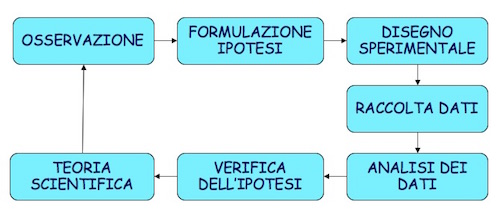
\includegraphics[width=0.75\linewidth]{_images/MSAMap} 

}

\caption{Il metodo scientifico Galileiano}\label{fig:figName11}
\end{figure}

Senza andare troppo in profondità, è importante notare due aspetti:

\begin{enumerate}
\def\labelenumi{\arabic{enumi}.}
\tightlist
\item
  il ruolo fondamentale dell'esperimento scientifico, che produce dati a
  supporto di ipotesi pre-esistenti;
\item
  lo sviluppo di teorie basate sui dati, che rimangono valide fino a che
  non si raccolgono altri dati che le confutano, facendo nascere nuove
  ipotesi che possono portare allo sviluppo di nuove teorie, più
  affidabili o più semplici.
\end{enumerate}

Insomma, l'ingrediente fondamentale di una prova scientifica è che è
supportata da un insieme dei dati sperimentali; di fatto, non esiste
scienza senza dati! Resta famoso l'aforisma ``In God we trust, all the
others bring data'', attribuito all'ingegnere e statistico americano W.
Edwards Deming (1999-1923), anche se pare che egli in realtà non l'abbia
mai pronunciato.

\section{Esperimenti buoni e
cattivi!}\label{esperimenti-buoni-e-cattivi}

Non tutti gli esperimenti sono buoni e, di conseguenza, non tutti i dati
sono buoni. In particolare, due sono gli elementi che possono portare a
dati di diversa affidabilità:

\begin{enumerate}
\def\labelenumi{\arabic{enumi}.}
\tightlist
\item
  Errore sperimentale
\item
  Campionamento
\end{enumerate}

Vediamo qualche dettaglio in più a proposito di questi due elementi.

\subsection{L'errore sperimentale}\label{lerrore-sperimentale}

Alla base della raccolta di dati sperimentali vi è un processo di
\textbf{misurazione}, attraverso la quale il fenomeno oggetto di studio
viene caratterizzato con appositi strumenti scientifici, più o meno
complessi. Il problema è che nessuna misura può essere considerata
precisa in senso assoluto, cioè perfettamente coincidente col valore
reale della grandezza misurata, che è destinato a rimanere un'entità
incognita e indeterminabile.

In particolare, in ogni esperimento scientifico esiste un potenziale
elemento di confusione che gli scienziati conoscono con il termine di
\textbf{errore sperimentale}, con la cui presenza è necessario
confrontarsi sempre e comunque.

Nel misurare una determinata grandezza fisica, indipendentemente dal
metodo scelto per la misura, possiamo sempre commettere due tipi di
errore: \textbf{sistematico} ed \textbf{accidentale (casuale)}.

L'errore sistematico è provocato da difetti intrinseci dello strumento o
incapacità peculiari dell'operatore e tende a ripetersi costantemente in
misure successive. Un esempio tipico è quello di una bilancia non
tarata, che tende ad aggiungere 20 grammi ad ogni misura che
effettuiamo. Per queste sue peculiarità, l'errore sistematico non è
quantificabile e deve essere contenuto al minimo livello possibile
tramite la perfetta taratura degli strumenti e l'adozione di metodi di
misura rigidamente standardizzati e accettati dalla comunità scientifica
mondiale.

L'errore accidentale (o casuale) è invece legato a fattori variabili nel
tempo e nello spazio, quali:

\begin{enumerate}
\def\labelenumi{\arabic{enumi}.}
\tightlist
\item
  \emph{malfunzionamenti accidentali dello strumento}. Si pensi ad
  esempio al rumore elettrico di uno strumento, che fa fluttuare i
  risultati delle misure effettuate;
\item
  \emph{imprecisioni o disattenzioni casuali dell'operatore}. Si pensi
  ad esempio ad un banale errore di lettura dello strumento, che può
  capitare soprattutto ad un operatore che esegua moltissime misure
  manuali con procedure di routine;
\item
  \emph{irregolarità} dell'oggetto da misurare\} unite ad una precisione
  relativamente elevata dello strumento di misura. Si pensi alla
  misurazione del diametro di un melone con un calibro: è facile che
  compaiano errori legati all'irregolarità del frutto o al fatto che
  l'operatore non riesce a misurare lo stesso nel punto in cui il suo
  diametro è massimo. Oppure, più semplicemente si pensi alla
  misurazione della produzione di granella di una certa varietà di
  frumento: anche ipotizzando di avere uno strumenti di misura perfetto
  e quindi esente da errore, la produzione mostrerebbe comunque una
  fluttuazione naturale da pianta a pianta, in base al patrimonio
  genetico e, soprattutto, in base alle condizioni di coltivazione che
  non possono essere standardizzate oltre ad un certo livello (si pensi
  alla variabilità del terreno agrario).
\end{enumerate}

Dato che queste imprecisioni sono assolutamente casuali è chiaro che le
fluttuazioni positive (misura maggiore di quella vera) sono altrettanto
probabili di quelle negative e tendono a presentarsi con la stessa
frequenza quando si ripetano le misure più volte. Di conseguenza,
l'errore sperimentale casuale può essere gestito attraverso la
\textbf{replicazione delle misure}: infatti, se ripeto una misura
soggetta a questo tipo di errore, nel lungo periodo gli errori positivi
e negativi tendono ad annullarsi reciprocamente e la media delle misure
effettuate tende quindi a coincidero con il valore reale della grandezza
da misurare.

\subsection{Il campionamento}\label{il-campionamento}

Se è vero, e la pratica sperimentale lo conferma, che ripetere le misure
porta ad ottenere molti risultati diversi, nasce il problema di capire
quante repliche sono necessarie. Se si ripensa a quanto detto finora,
dovrebbe risultare evidente che, per ottenere misure pari all'effettivo
(reale) valore della grandezza da misurare, bisognerebbe effettuare
infinite repliche. Tuttavia è altrettanto evidente che questo
procedimento è totalmente improponibile!!!

Qual è la strada seguita dagli scenziati, quindi? E' quella di
raccogliere un numero finito di misure, sufficientemente basso da essere
compatibile con le umane risorse di tempo e denaro, ma sufficientemente
alto da essere giudicato attendibile. Qualunque sia questo valore
finito, è evidente che ci troviamo difronte solo ad un campione delle
infinite misure che avremmo dovuto fare, ma che non abbiamo fatto. La
domanda è: questo campione è rappresentativo o no? E' in grado di
descrivere adeguatamente la realtà? E' possibile che gli errori
sperimentali positivi e negativi non si siano annullati tra loro,
confondendosi con l'effetto biologico in studio? In altre parole:
possiamo fidarci dei dati che abbiamo raccolto?

La possibilità di raccogliere dati sbagliati è tutt'altro che remota.
Gli scienziati american Pons e Fleischmann il 23 Marzo del 1989
diffusero pubblicamente la notizia di essere riusciti a riprodurre la
fusione nucleare fredda, causando elevatissimo interesse nella comunità
scientifica. Purtroppo le loro misure erano vizite da una serie di
problemi e il loro risultato fu clamorosamente smentito da esperimenti
successivi.

\begin{figure}

{\centering 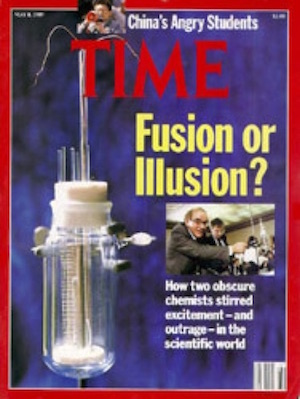
\includegraphics[width=0.5\linewidth]{_images/FalseResults} 

}

\caption{Conseguenze di un esperimento sbagliato}\label{fig:figName2}
\end{figure}

\section{Scienza = metodo}\label{scienza-metodo}

Insomma, la scienza deve essere basata sui dati, ma i dati contengono
inevitabili fonti di incertezza, legate all'errore sperimentale e al
processo di campionamento. Come si può procedere in queste condizioni?
Il punto fondamentale è quello di adottare un metodo sperimentale che
consenta di ottenere dati \textbf{il più affidabili possibile}. Insomma,
questa semplice affermazione significa che bisogna fare eseperimenti ben
condotti, precisi, seguendo procedure standardizzate e/o largamente
condivise dalla comunità scientifica.

Certo è che, per quanto detto in precedenza, il fatto che i dati
provengano da un processo di campionamento impedisce, di fatto, di
ottenere un'affidabilità totale. Cosa succederebbe se ripetessimo
l'esperimento?

Insomma, bisogna fare alcune considerazioni, che elenco di seguito:

\begin{enumerate}
\def\labelenumi{\arabic{enumi}.}
\tightlist
\item
  in primo luogo si dovrà accettare il fatto che, contrariamente a
  quanto si potrebbe o vorrebbe credere, non esistono prove scientifiche
  totalmente certe, ma l'incertezza è un elemento intrinseco della
  scienza.
\item
  In secondo luogo si dovranno utilizzare gli strumenti della statistica
  necessari per quantificare l'incertezza residua, che dovrà essere
  sempre riportata a corredo dei risultati di ogni esperimento
  scientifico.
\item
  Ogni risultato sarà quindi valutato dalla comunità scientifica sullo
  sfondo della sua incertezza, seguendo alcune regole di natura
  probabilistica che consentono di stabilire se la prova scientifica è
  sufficientemente forte per essere considerata tale.
\end{enumerate}

Un elemento fondamentale di valutazione della bontà di un esperimento e
dei dati da esso ottenuti sta nella cosiddetta \textbf{replicabilità},
cioè nella probabilità di ottenere risultati molto simili (se non
uguali) replicando l'esperimento in condizioni analoghe. Per valutare se
un esperimento è replicabile è necessario che questo sia descritto con
un grado di dettaglio tale da permettere a chinque di ripeterlo,
ottenendo risultati comparabili e non contraddittori. Nessun risultato
di cui non sia provata la riproducibilità è da considerarsi valido.

E'chiaro comunque che ogni esperimento può essere smentito. Questo non è
un problema: la scienza è pronta a considerare una prova scientifica
valida fino a che non si raccolgono dati altrettanto affidabili che la
confutino. In questo caso, si abbandona la teoria confutata e si
abbraccia la nuova. L'abbandono può anche non essere totale: ad esempio
la teoria gravitazionale di Newton è ancora oggi valida per molto
situazioni pratiche, anche se è stata abbandonata in favore della teoria
della relatività, che spiega meglio il moto dei corpi ad altissime
velocità.

In effetti, la scienza considere sempre con attenzione il principio del
rasoio di Occam, per il quale si accetta sempre la teoria più semplice
per interpretare una dato fenomeno, riservando le teorie più complesse
alle situazioni più difficili, che giustificano tale livello di
complessità.

\section{Chi valuta se un esperimento è
attendibile?}\label{chi-valuta-se-un-esperimento-e-attendibile}

Quanto detto finora vorrebbe chiarire come il punto centrale della
scienza non è la certezza delle teorie, bensì il metodo che viene
utilizzato per definirle. Ognuno di noi è quindi responsabile di
verificare che le informazioni in suo possesso siano `scientificamente'
attendibili, cioè ottenute con un metodo sperimentale adeguato. Il fatto
è che non sempre siamo in grado di compiere questa verifica, perché non
abbiamo strumenti `culturali' adeguati, se non nel ristretto ambito
delle nostre competenze professionali. Come fare allora?

L'unica risposta accettabile è quella di controllare l'attendibilità
delle fonti di informazione. In ambito biologico, le riviste autorevoli
sono caratterizzate dal procedimento di `\emph{peer review}', nel quale
i manoscritti scientifici, prima della pubblicazione, sono sottoposti ad
un comitato editoriale ed assegnati ad un `editor', il quale legge il
lavoro e contemporaneamente lo invia a due o tre scienziati anonimi e
particolarmente competenti in quello specifico settore scientifico
(\emph{reviewers} o revisori).

I revisori, insieme all'\emph{editor}, compiono un attento lavoro di
esame e stabiliscono se l'evidenza scientifica presentata è
sufficientemente `forte'. Le eventuali critiche vengono presentate
all'autore, che è tenuto a rispondere in modo convincente, anche
ripetendo gli esperimenti se necessario. Il processo richiede spesso
interi mesi ed è abbastanza impegnativo per uno scenziato. E' piuttosto
significativa l'immagine presentata in
\href{http://scienceblogs.com/startswithabang/2013/06/07/the-4-jobs-of-a-referee-in-peer-review/}{scienceBlog.com},
che allego qui.

\begin{figure}

{\centering 
\includegraphics[width=0.75\linewidth]{_images/PeerReview} 

}

\caption{Il processo di peer review}\label{fig:figName3}
\end{figure}

In sostanza il meccanismo di \emph{peer review} è l'analogo scientifico
di un processo, nel quale l'inputato (lavoro scientifico) viene assolto
(rilasciato, leggi: rigettato) in presenza di qualunque ragionevole
dubbio metodologico. Attenzione: il dubbio che non deve esistere è
quello metodologico, dato che il dubbio sul risultato non può essere
allontanato completamente e i reviewer controlleranno solo che esso si
trovi al disotto della soglia massima, stabilita con metodiche
statistiche.

Questo procedimento, se effettuato con competenza, dovrebbe aiutare a
separare la scienza dalla pseudo-scienza e, comunque, ad eliminare la
gran parte degli errori metodologici dai lavori scientifici.

\section{Il metodo sperimentale}\label{il-metodo-sperimentale}

Almeno in ambito biologico, la definizione del metodo sperimentale è
fondamentalmente attribuita allo scienziato inglese Ronald Fisher
(1890-1962), che l'ha esplicitata nel suo famoso testo del 1935 (The
design of experiments). Mi sembra opportuno riassumerla nelle tre
espressioni `chiave': controllo locale degli errori, replicazione e
randomizzazione. Si tratta di:

\begin{enumerate}
\def\labelenumi{\arabic{enumi}.}
\tightlist
\item
  contenere al massimo possibile l'errore sperimentale, con l'adozione
  di tecniche opportune, in modo da separare le fonti di variabilità,
  isolando qualla oggetto di studio (controllo locale degli errori);
\item
  replicare le misure più volte (replicazione)
\item
  Scegliere le unità sperimentali da misurare in modo totalmente
  casuale, così da avere un campione rappresentativo ed evitare di
  confondere gli effetti prodotti dall'errore sperimentale con quelli
  prodotti dal fenomeno biologico oggetto di studio (randomizzazione)
\end{enumerate}

Vediamo ora un'esempio banale di come procedere.

\section{Metodi sperimentali validi ed
invalidi}\label{metodi-sperimentali-validi-ed-invalidi}

Immaginiamo un ricercatore che abbia un'idea brillante: egli ha
inventato un nuovo fertilizzante `prodigioso'. E' evidente che non può
presentarsi alla comunità scientifica declamando le doti di questo
fertilizzante, in quanto egli verrebbe immediatamente esposto al
pubblico ludibrio, perchè sta presentando delle opinioni, non delle
evidenze scientifiche (almeno, così dovrebbe essere, in una società
sana\ldots{} purtroppo in un'era di pseudo-scienza siamo sempre pronti a
dar credito a chiunque, senza un'adeguata dose di scetticismo\ldots{} )

\subsection{Primo esperimento}\label{primo-esperimento}

Come ogni scenziato, egli deve raccogliere dati. E lo fa, organizzando
un esperimento, nel quale prende un campo di mais e lo fertilizza con il
suo nuovo composto, ritraendo una produzione del 20\% superiore a quella
usuale. Ovviamente, se prova a pubblicare questa notizia, il suo lavoro
verrà certamente (si spera\ldots{}) rigettato, in quanto rimane il
dubbio su chi sia la causa dell'effetto riscontrato: il fertilizzante?
il clima dell'anno di prova? il suolo? la varietà di mais impiegata? E'
chiaro che questo non è un esperimento controllato: il campo trattato e
quello non trattato (riferimento) differiscono per molte altre
caratteristiche, oltre al fertilizzante impiegato.

\subsection{Secondo esperimento}\label{secondo-esperimento}

A questo punto il ricercatore pianifica un esperimento comparativo
controllato: prende due campi di mais, vicini, con lo stesso terreno,
semina la stessa varietà di mais e coltiva i due campi esattamente nello
stesso modo, con l'unica differenza che in uno di essi somministra il
fertilizzante in studio (campo trattato) e nell'altro no (testimone o
controllo). Alla fine osserva che il campo trattato produce 130
tonnellate per ettaro, mentre quello non trattato ne produce 115 e
conclude che il nuovo fertilizzante è efficace (+ 12\% circa). Infatti
egli ritiene che, dato che i due campi sono totalmente uguali,
l'incremento di produzione non possa che essere attribuito al
fertilizzante. Scrive un report, che, purtroppo, viene rigettato.

Anche se questo secondo esperimento è meglio del primo, permane tuttavia
il dubbio che l'effetto si sia prodotto per caso. Potrebbe infatti
esserci stata una qualche situazione non osservata che ha avvantaggiato
uno dei due campi. Ad esempio un attacco di insetti, una carenza idrica,
o qualsivoglia altra situazione. Questo vi sembra improbabile? Non
importa, con una sola osservazione il ricercatore non è in grado di
provare che il risultato è replicabile.

\subsection{Terzo esperimento}\label{terzo-esperimento}

Avendo imparato la lezione, il ricercatore fa un nuovo esperimento,
utilizzando stavolta otto campi: quattro trattati e quattro non
trattati. Anche in questo caso osserva un incremento produttivo medio
del 12\% circa ed è sicuro che l'effetto è replicabile, perché lo ha
osservato più volte. Purtroppo, anche questo esperimento non viene
considerato affidabile e, di conseguenza, il lavoro non è pubblicabile.
Stavolta il problema è che il ricercatore, senza accorgersene, ha scelto
i campi trattati con un criterio sistematico: procedendo da sinistra
verso destra, ha trattato un campo ed ha lasciato non trattato quello
immediatamente contiguo alla sua destra e così via. Di conseguenza, i
campi trattati sono tutti a sinistra di quelli non trattati, il che crea
un ragionevole dubbio: e se vi fosse un gradiente di fertilità da destra
verso sinistra? Questo potrebbe dare origine ad una produttività
maggiore dei campi a destra, rispetto a quelli a sinistra,
indipendentemente dall'effetto del concime. In presenza di questo
`ragionevole' dubbio, la prova non può avere valenza scientifica.

\subsection{Quarto esperimento: quello
buono}\label{quarto-esperimento-quello-buono}

Il ricercatore prende allora otto campi ed assegna il trattamento a
quattro di essi, scelti in modo totalmente casuale. In questo caso è
sicuro che, anche se vi fosse un qualche elemento estraneo di confusione
(gradiente di fertilità, attacco di insetti\ldots{}), esso dovrebbe
colpire le unità sperimentali casualmente disposte senza creare vantaggi
particolari all'uno o all'altro dei due trattamenti. Ovviamente egli non
è certo (e non può esserlo) che l'esperimento sia del tutto attendibile;
infatti potrebbe essere stato così sfortunato che un qualche elemento
estraneo ignoto si è accanito proprio sulle parcelle non trattate,
danneggiandone la produttività. Solo che, grazie alla scelta casuale,
questa evenienza diviene altamente improbabile, così da rendere i dubbi
irragionevoli. In questo caso l'esperimento è controllato, replicato e
randomizzato e il risultato ottenuto, in quanto ragionevolmente
attendibile, può essere pubblicato.

\section{Incertezza residua}\label{incertezza-residua}

Insomma, un esperimento valido è controllato, replicato e randomizzato.
Tuttavia le misure raccolte sono poche e sono solo un campione di tutte
quelle possibili. Infatti il nostro ricercatore ha usato otto campi, ma
ne avrebbe potuti usare 16, 32 e così via. Rimane quindi il dubbio, che,
se facessimo altre misure (cioè ampliassimo il campione), queste
potrebbero invalidare i risultati ottenuti fino a quel momento.

Se mi è concesso un paragone calcistico, è un po' come chiedersi come
finirà una partita di calcio dopo aver assistito solo al primo tempo: in
alcune circostanze, quando una delle due squadre ha mostrato una chiara
superiorità, la previsione è abbastanza facile, mentre in altre
circostanze l'equivalenza dei valori in campo la rende alquanto
difficile. In tutti i casi, si tratta solo di una previsione, che può
essere sempre smentita alla prova dei fatti.

Anche la scienza funziona così. Noi osserviamo solo il primo tempo, che,
nel caso del nostro ricercatore, consiste di otto misure. Osserviamo che
le quattro misure del fertilizzato sono tutte in modo consistente molto
più alte di quelle del non trattato e quindi possiamo concludere, con
ragionevole certezza, che il fertilizzante è efficace. In altri casi,
dove la produzione media del trattato fosse solo lievemente più alta del
non trattato, l'esperimento potrebbe essere inconclusivo, cioè incapace
di dare risultati attendibili sull'effettiva efficacia del nostro
fertilizzante. Avremmo quindi bisogno di fare altre prove di conferma.

\section{Il ruolo della statistica}\label{il-ruolo-della-statistica}

Nell'ottica esposta in precedenza, la statistica ci fornisce gli
strumenti per riassumere le misure effettuate, calcolarne l'incertezza e
rappresentare la forza dell'evidenza scientifica, in modo da poter
prendere decisioni sull'efficacia dei trattamenti e sull'esigenza di
ulteriori verifiche. Imparare a conoscere e comprendere questi strumenti
statistici è l'obiettivo di questo corso.

\section{Conclusioni}\label{conclusioni}

In conclusione, possiamo ripartire dalla domanda iniziale: ``Che cosa è
la scienza?'', per rispondere che è scienza tutto ciò che è supportato
da dati che abbiano passato il vaglio della \emph{peer review},
dimostrando di essere stati ottenuti con un procedimento sperimentale
privo di vizi metodologici e di essere sufficientemente affidabili in
confronto alle fonti di incertezza cui sono associati.

Qual è il \emph{take-home message} di questo capitolo? Fidatevi solo
delle riviste scientifiche attendibili, cioè quelle che adottano un
serio processo di \emph{peer review} prima della pubblicazione.

\chapter{Esperimenti validi ed
invalidi}\label{esperimenti-validi-ed-invalidi}

\section{Definizioni}\label{definizioni}

La ricerca scientifica trova la sua unità elementare nell'esperimento,
cioè un \emph{processo investigativo, con il quale, seguendo un adeguato
protocollo, si osserva e si misura la risposta prodotta da uno o più
`stimoli' sperimentali nei soggetti coinvolti nello studio}. Raramente
gli esperimenti sono isolati, più spesso fanno parte di uno sforzo
collettivo organizzato, generalmente identificato con il nome di
progetto di ricerca.

Ogni esperimento deve essere attentamente pianificato. Infatti, sappiamo
che la variabilità esistente tra soggetti sperimentali, il
campionamento, le irregolarità di misura e molti altri fattori
perturbativi ci impediscono di osservare la realtà con assoluta
precisione. E' come se osservassimo un fenomeno attraverso una sorta di
lente deformante, che ci impone di adottare un metodo sperimentale
rigoroso, per evitare di attribuire al fenomeno in studio effetti che
sono invece puramente casuali o, anche peggio, dovuti a qualche elemento
ignoto.

In particolare, gli esperimenti debbono essere:

\begin{enumerate}
\def\labelenumi{\arabic{enumi}.}
\tightlist
\item
  Precisi
\item
  Accurati
\item
  Replicabili/Riproducibili
\end{enumerate}

In mancanza di questi requisiti, al termine dell'esperimento possono
rimanere dubbi sui risultati, tali da inficiare la validità delle
conclusioni raggiunte. Cerchiamo di chiarire cosa si intende con questi
tre termini.

\textbf{Precisione}. Con il termine precisione intendiamo due cose: la
prima è relativa al numero di decimali che ci fornisce il nostro
strumento di misura. E'evidente, ad esempio, come un calibro sia più
preciso di un metro da sarto. Oltre a questo concetto abbastanza
intuitivo di precisione ce n'è un altro, specificatamente legato agli
esperimenti scientifici, nei quali le misure vengono ripetute più volte.
La precisione di un esperimento non è altro che la variabilità dei
risultati tra una replica e l'altra.

\textbf{Accuratezza}. La precisione, da sola, non garantisce che
l'esperimento sia affidabile. Abbiamo menzionato nel capitolo precedente
che l'errore sperimentale può essere casuale o sistematico. Quest'ultimo
può essere dovuto, per esempio, ad uno strumento non accurato che
sovrastima tutte le misure. In questo caso, posso ripetere cento volte
la misura, ottenendo sempre lo stesso risultato, molto preciso, ma
totalmente inaffidabile, nel senso che non riflette la misura reale del
soggetto. L'accuratezza è proprio la capacità di un procedimento di
misura di restituire il valore vero del soggetto misurato, anche se come
media di un numero molto elevato di replicazioni. L'accuratezza è molto
più importante della precisione: infatti una misura accurata, ma
imprecisa, riflette bene la realtà, anche se in modo vago. Al contrario,
una misura precisa, ma inaccurata ci porta completamente fuori strada,
perchè non riflette la realtà! Un esperimento/risultato non accurato si
dice `distorto' (\emph{biased}).

\textbf{Replicabilità/Riproducibilità}. Un esperimento o una misura sono
replicabili se, quando ripetuti in condizioni assolutamente analoghe
(stessi soggetti, ambiente, strumenti\ldots{}), restituiscono risultati
equivalenti. Alcuni biostatistici distinguono la replicabilità dalla
riproducibilità, in quanto considerano quest'ultima come la possibilità
di ottenere risultati equivalenti ripetendo una misura in condizioni
diverse (diversi soggetti, diverso ambiente\ldots{}). E'evidente che un
esperimento può essere totalmente accurato e replicabile, ma non
riproducibile con soggetti e condizioni ambientali diverse. Se è così,
le conclusioni raggiunte, anche se accurate, non sono generalizzabili.

\section{Elementi fondamentali del disegno
sperimentale}\label{elementi-fondamentali-del-disegno-sperimentale}

La metodica di organizzazione di un esperimento prende il nome di
\emph{disegno sperimentale} e deve essere sempre adeguatamente
formalizzata tramite la redazione di un \emph{protocollo sperimentale}
sufficientemente dettagliato da consentire a chiunque la replicazione
dell'esperimento e la verifica dei risultati.

Le basi del disegno sperimentale si fanno in genere risalire a Sir
Ronald A. Fisher, vissuto in Inghilterra dal 7 Febbraio 1890 al 29
luglio 1962. Laureatosi nel 1912, lavora come statistico per il comune
di Londra, fino a quando diviene socio della prestigiosa Eugenics
Education Society di Cambridge, fondata nel 1909 da Francis Galton,
cugino di Charles Darwin. Dopo la fine della guerra, Karl Pearson gli
propone un lavoro presso il rinomato Galton Laboratory, ma egli non
accetta a causa della profonda rivalità esistente tra lui e Pearson
stesso. Nel 1919 viene assunto presso la Rothamsted Experimental
Station, dove si occupa dell'elaborazione dei dati sperimentali e, nel
corso dei successivi 7 anni, definisce le basi del disegno sperimentale
ed elabora la sua teoria della ``analysis of variance''. Il suo libro
più importante è ``The design of experiment'', del 1935. E' sua la
definizione delle tre componenti fondamentali del disegno sperimentale:

\begin{enumerate}
\def\labelenumi{\arabic{enumi}.}
\tightlist
\item
  controllo degli errori;
\item
  replicazione;
\item
  randomizzazione.
\end{enumerate}

Abbiamo già menzionato questi aspetti nel capitolo precedente; ora li
riprendiamo in esame con maggior dettaglio.

\subsection{Primo elemento: controllo degli
errori}\label{primo-elemento-controllo-degli-errori}

Controllare gli errori, o, analogamente, eseguire un esperimento
controllato signfica fondamentalmente due cose:

\begin{enumerate}
\def\labelenumi{\arabic{enumi}.}
\tightlist
\item
  adottare provvedimenti idonei ad evitare le fonti di errore,
  mantenendole al livello più basso possibile (alta precisione);
\item
  agire in modo da isolare l'effetto in studio (accuratezza), evitando
  che si confonda con effetti casuali e di altra natura. Ad esempio, se
  dobbiamo confrontare due fitofarmaci, dobbiamo fare in modo che i
  soggetti inclusi nell'esperimento differiscano tra di loro solo per il
  fitofarmaco impiegato e non per altro.
\end{enumerate}

Declinare questi principi richiederebbe una vita di esperienza! Vogliamo
solo ricordare alcuni aspetti fondamentali, relativi all'importanza di:

\begin{enumerate}
\def\labelenumi{\arabic{enumi}.}
\tightlist
\item
  Campionamento rappresentativo
\item
  Omogeneità
\item
  Rigore metodologico
\item
  Evitare le `intrusioni'
\end{enumerate}

\subsubsection{Campionamento
rappresentativo}\label{campionamento-rappresentativo}

E' evidente che il primo requisito di un esperimento è una corretta
scelta delle unità sperimentali, cioè le più piccole unità che ricevono
lo `stimolo' rappresentato dal trattamento, in modo indipendente da
tutte le altre.

Cerchiamo subito di comprendere una fondamentale distinzione tra unità
sperimentali e unità osservazionali. Le prime sono state definite nel
paragrafo precedente; le seconde sono quelle che costituiscono l'oggetto
della misura e possono anche non coincidere con le prime. Ad esempio:
immaginiamo di trattare con un diserbante due vasetti, in modo
indipendente l'uno dall'altro. Immaginiamo poi di pesare singolarmente
le quattro piante di ciascun vasetto; in questa situazione, il vasetto è
l'unità sperimentale, le piante sono invece le unità osservazionali.
L'elemento discriminante di questo esempio è l'indipendenza: mentre le
unità sperimentali hanno ricevuto il trattamento in modo indipendente
l'una dall'altra, le unità osservazionali no. Questa differenza è
fondamentale, per motivi che vedremo più avanti.

Le unità sperimentali possono essere di varia natura (persone, semi,
piante, animali\ldots{}); nel caso degli esperimenti di campo, le unità
sperimentali sono dette \textbf{parcelle} e sono un pezzetto di terreno,
di varia forma e dimensione.

\begin{figure}

{\centering 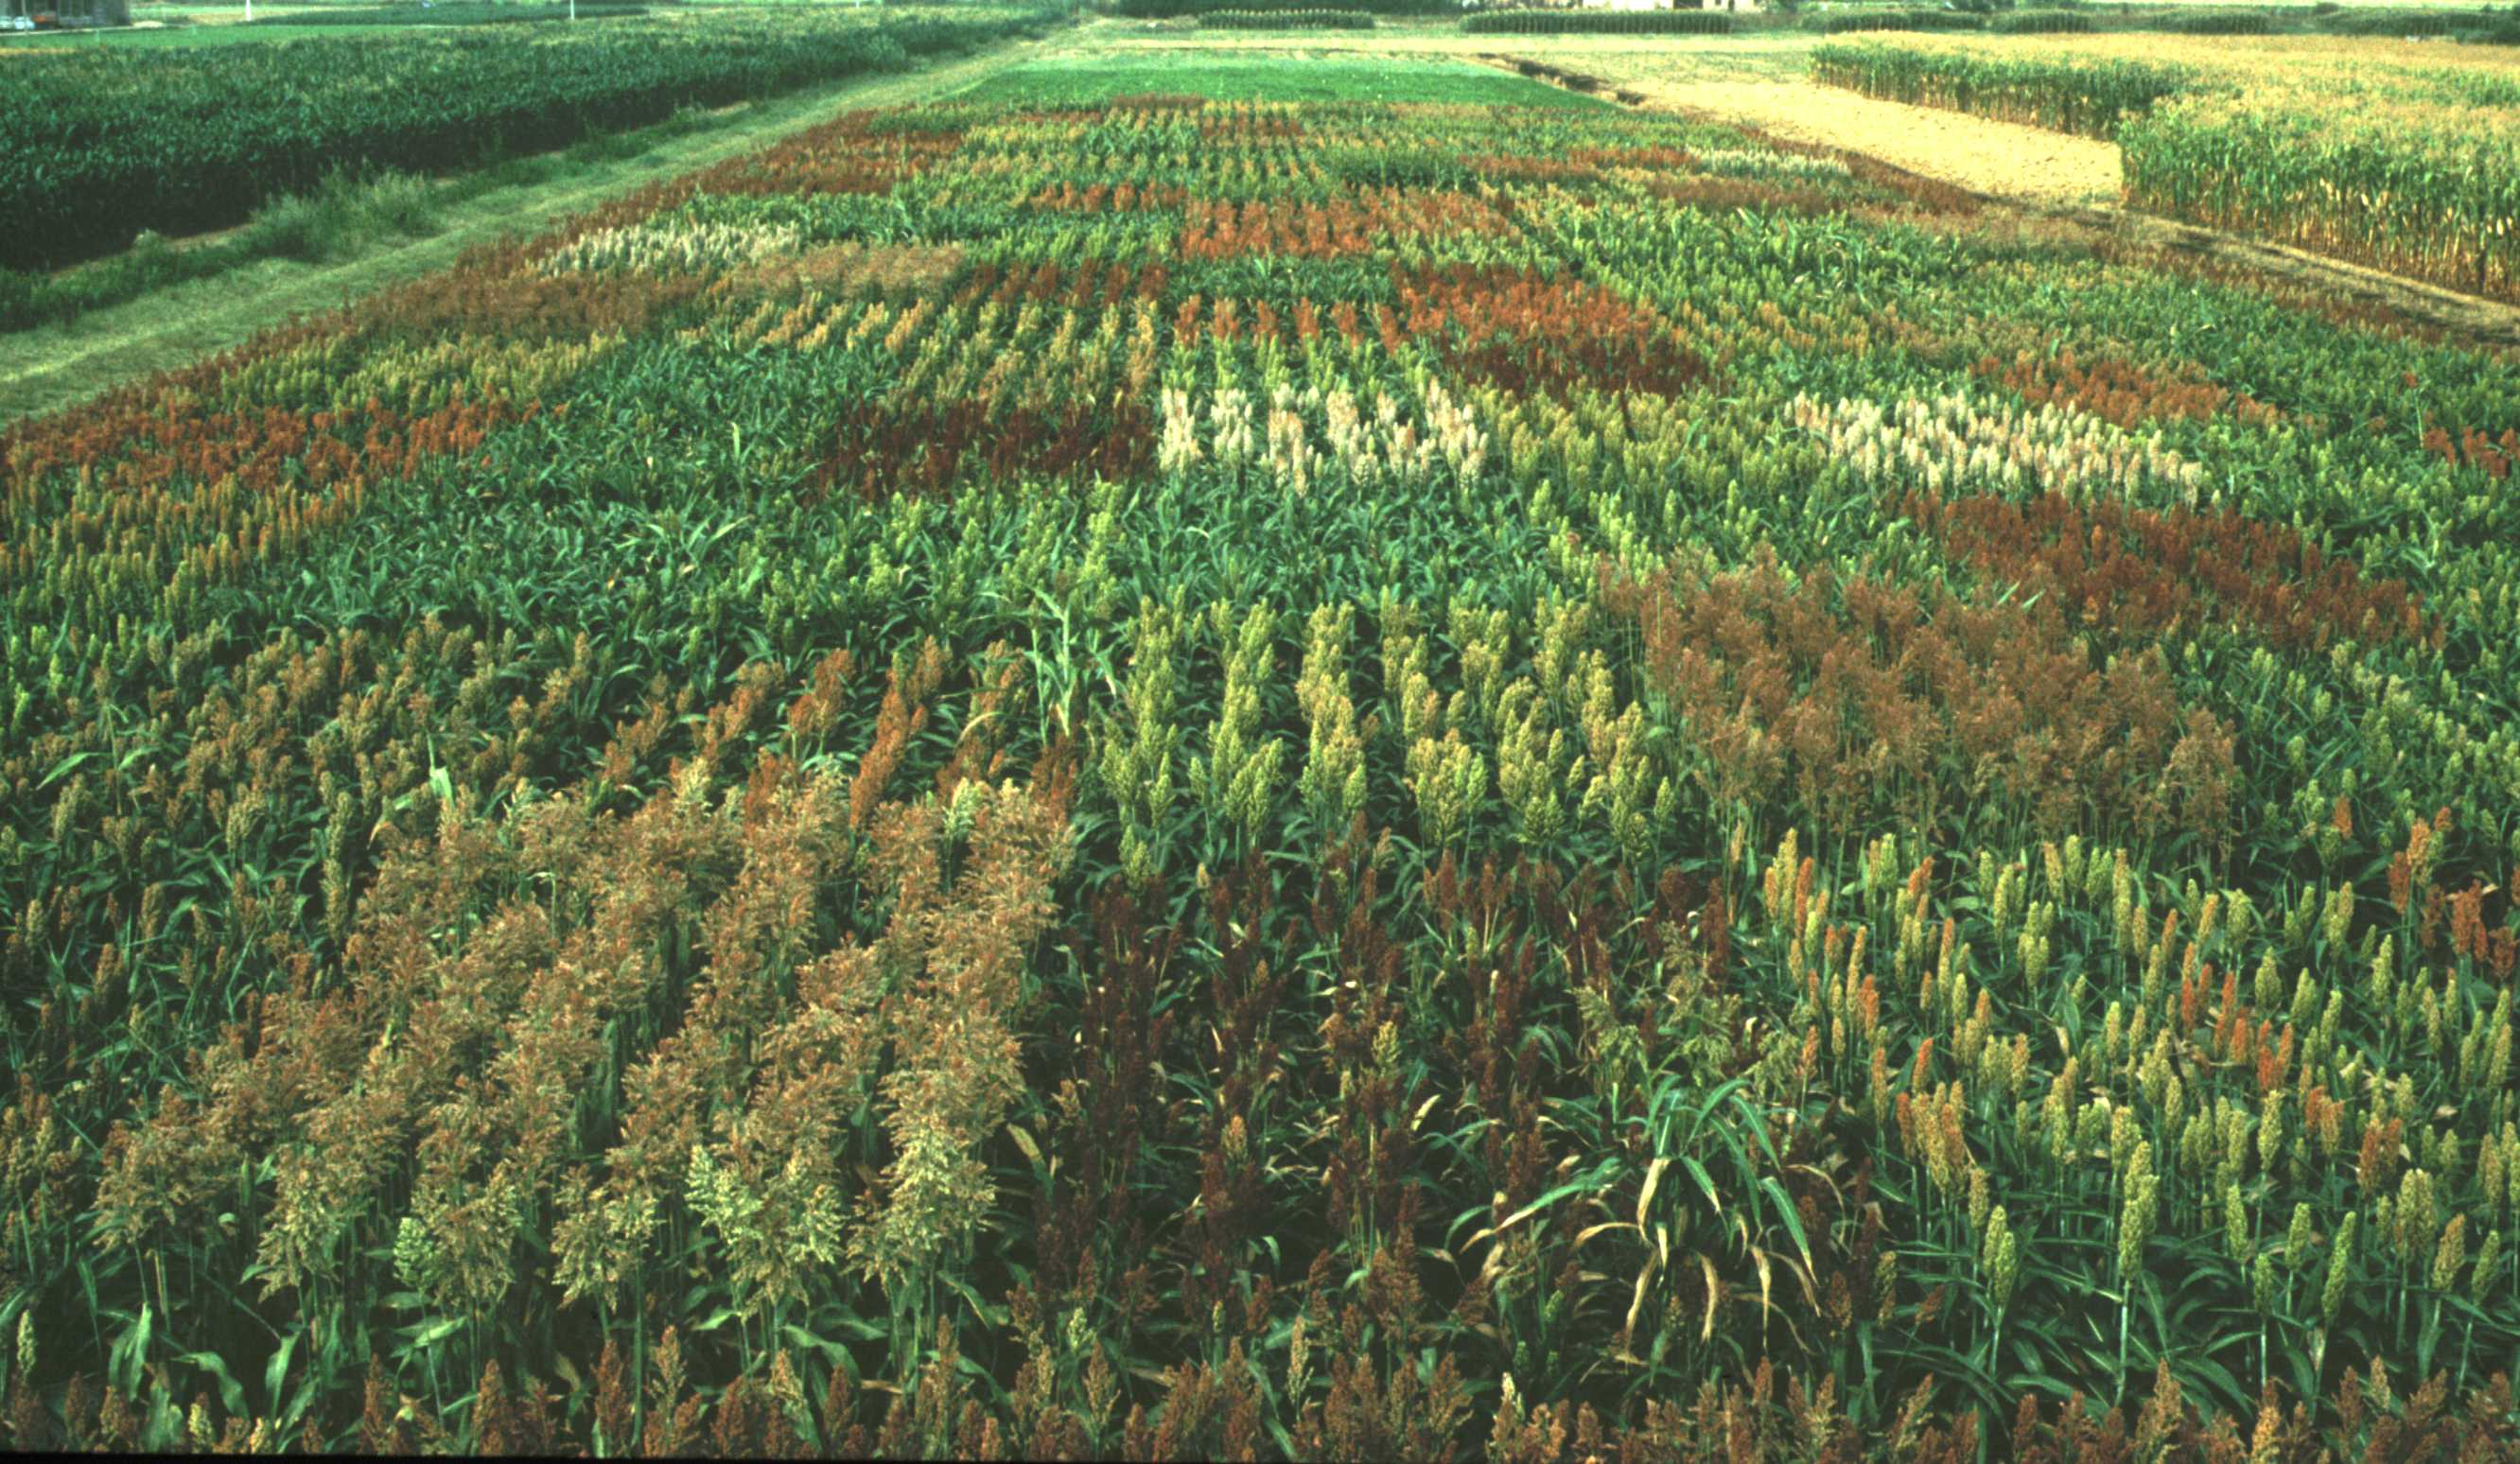
\includegraphics[width=0.9\linewidth]{_images/SorgoProveVarietali} 

}

\caption{Una prova sperimentale in campo (Foto D. Alberati)}\label{fig:figName21}
\end{figure}

Le unità sperimentali sono scelte per campionamento, che è un elemento
fondamentale dell'esperimento ed avviene all'interno della cosiddetta
\textbf{cornice di campionamento}, cioè la popolazione da cui io devo
campionare. Quest'ultima deve essere scelta in modo adeguato: devo
effettuare un esperimento valido per l'Italia centrale, per una località
particolare, per tutta Italia? Devo fare un esperimento che riguarda una
stalla in particolare o tutte le stalle dove si allevano bovini? Di
quale razza? La \textbf{cornice di campionamento} è fondamentale in
quanto il campione, se ben scelto, rappresenta la popolazione da cui
deriva, non altre.

E' superfluo dire che, nell'ambito della cornice di campionamento, il
campione deve essere prescelto in modo da essere rappresentativo,
altrimenti l'esperimento è invalido. Dare indicazioni su come si possa
assicurare la rappresentatività del campione è impossibile, in quanto
ciò dipende dalla tipologia di esperimento. Il campionamento è
fondamentale nelle scienze sociali, dove vengono applicate tecniche
particolari, come il campionamento randomizzato (completamente casuale),
quello stratificato (che avviene all'interno di strati omogenei della
popolazione), quello sistematico (es. prendo il primo soggetto che
incontro e poi ne prendo uno ogni dieci), ecc.. Chi fosse interessato
può reperire informazioni in letteratura (Daniel
\protect\hyperlink{ref-DanielSamplingessentialspractical2011}{2011}).

Nelle scienze agrarie e biologiche, il campionamento si giova di
metodologie meno `raffinate' e spesso si prendono i soli soggetti
disponibili (le parcelle di un campo sperimentale o gli animali della
stalla del Dipartimento in cui si opera\ldots{}). E' chiaro che, pur non
eseguendo una vera e propria operazione di campionamento, non bisogna
scordare che i soggetti sperimentali rappresentano solo la popolazione
da cui sono stati estratti. Ad esempio, se faccio un esperimento in
un'azienda sperimentale del centro Italia, i risultati che ottengo sono
riferibili solo a questa zona geografica; se volessi conclusioni più
generali dovrei cercare anche altre aziende in situazioni
pedo-climatiche diverse.

\subsubsection{Omogeneità}\label{omogeneita}

Anche in questo caso, l'importanza di scegliere soggetti uniformi e
posti in un ambiente uniforme (nello spazio e nel tempo) è evidente.
Bisogna comunque tener presente che i risultati di un esperimento si
estendono alla popolazione da cui il campione è estratto e della quale
esso rappresenta le caratteristiche. Esperimenti nei quali si restringe
il campo di variabilità dei soggetti e dell'ambiente sono certamente più
precisi, ma forniscono anche risultati meno generalizzabili.
L'importante è avere ben chiaro su quale è il campo di validità che si
vuole dare ai risultati. Ad esempio, se si vuole ottenere un risultati
riferito alla collina umbra, bisognerà scegliere soggetti che
rappresentano bene la variabilità pedo-climatica della collina Umbra; né
più, né meno.

\subsubsection{Rigore}\label{rigore}

Direi che questo aspetto è ovvio e non richiede commenti particolari:
una ricerca deve essere condotta `a regola d'arte'. E' evidente che, ad
esempio, se vogliamo sapere la cinetica di degradazione di un erbicida a
20 °C dovremo realizzare una prova esattamente a quella temperatura, con
un erbicida uniformemente distribuito nel terreno, dentro una camera
climatica capace di un controllo perfetto della temperatura. Gli
strumenti dovranno essere ben tarati e sarà necessario attenersi
scrupolosamente a metodi validati e largamente condivisi.

Tuttavia, a proposito di rigore, non bisogna scordare quanto diceva C.F.
Gauss a proposito della precisione nei calcoli, e che può essere anche
riferito al rigore nella ricerca : ``\emph{Manca di mentalità matematica
tanto chi non sa riconoscere rapidamente ciò che è evidente, quanto chi
si attarda nei calcoli con una precisione superiore alla necessità}''

\subsubsection{\texorpdfstring{Evitare le `intrusioni
demoniache'}{Evitare le intrusioni demoniache}}\label{evitare-le-intrusioni-demoniache}

Secondo Hurlbert (1984), le intrusioni sono eventi totalmente casuali
che impattano negativamente con un esperimento in corso. E' evidente
che, ad esempio, un'alluvione, l'attacco di insetti o patogeni, la
carenza idrica hanno una pesante ricaduta sulla precisione di un
esperimento e sulla sua riuscita. Nello stesso lavoro, Hurlbert usa il
termine `intrusione demoniaca' per indicare quelle intrusioni che, pur
casuali, avrebbero potuto essere previste con un disegno più accurato,
sottolineando in questo caso la responsabilità dello sperimentatore.

Un esempio è questo: uno sperimentatore vuole studiare l'entità della
predazione dovuta alle volpi e quindi usa campi senza staccionate (dove
le volpi possono entrare) e campi protetti da staccionate (e quindi
liberi da volpi). Se le staccionate, essendo utilizzate dai falchi come
punto d'appoggio, finiscono per incrementare l'attività predatoria di
questi ultimi, si viene a creare un'intrusione demoniaca, che rende
l'esperimento distorto. Il demonio, in questo caso, non è il falco, che
danneggia l'esperimento, ma il ricercatore stesso, che non ha saputo
prevedere una possibile intrusione.

\subsection{Secondo elemento:
replicazione}\label{secondo-elemento-replicazione}

In ogni esperimento, i trattamenti dovrebbe essere replicati su due o
più unità sperimentali. Ciò permette di:

\begin{enumerate}
\def\labelenumi{\arabic{enumi}.}
\tightlist
\item
  dimostrare che i risultati sono replicabili (ma non è detto che siano
  riproducibili!)
\item
  rassicurare che eventuali circostanze aberranti casuali non abbiano
  provocato risultati distorti
\item
  misurare l'errore sperimentale, come variabilità di risposta tra
  repliche trattate nello stesso modo (precisione dell'esperimento)
\item
  incrementare la precisione dell'esperimento (più sono le repliche più
  l'esperimento è preciso, perché si migliora la stima della
  caratteristica misurata, diminuendo l'incertezza)
\end{enumerate}

Per poter essere utili, le repliche debbono essere indipendenti, cioè
debbono \textbf{aver subito tutte le manipolazioni necessarie per
l'allocazione del trattamento in modo totalmente indipendente l'una
dall'altra}. Le manipolazioni comprendono tutte le pratiche necessarie,
come ad esempio la preparazione delle soluzioni, la diluizione dei
prodotti, ecc..

La manipolazione indipendente è fondamentale, perché in ogni parte del
processo di trattamento possono nascondersi errori più o meno grandi,
che possono essere riconosciuti solo se colpiscono in modo casuale le
unità sperimentali. Se la manipolazione è, anche solo in parte, comune,
questi errori colpiscono tutte le repliche allo stesso modo, diventano
sistematici e quindi non più riconoscibili. Di conseguenza, si inficia
l'accuratezza dell'esperimento. Quando le repliche non sono
indipendenti, si parla di \textbf{pseudorepliche}, contrapposte alle
\textbf{repliche vere}.

Il numero di repliche dipende dal tipo di esperimento: più sono e meglio
è, anche se è necessario trovare un equilibrio accettabile tra
precisione e costo dell'esperimento. Nella sperimentazione di campo, due
repliche sono poche, tre appena sufficienti, quattro costituiscono la
situazione più comune, mentre un numero maggiore di repliche è
abbastanza raro, non solo per la difficoltà di seguire l'esperimento, ma
anche perché aumentano la dimensione della prova e, di conseguenza, la
variabilità del terreno.

\subsection{Terzo elemento:
randomizzazione}\label{terzo-elemento-randomizzazione}

L'indipendenza di manipolazione non garantisce da sola un esperimento
corretto. Infatti potrebbe accadere che le caratteristiche innate dei
soggetti, o una qualche `intrusione' influenzino in modo sistematico
tutte le unità sperimentali trattate nello stesso modo, così da
confondersi con l'effetto del trattamento. Un esempio banale è che
potremmo somministrare un farmaco a quattro soggetti in modo totalmente
indipendente, ma se i quattro soggetti fossero sistematicamente più alti
di quelli non trattati finiremmo per confondere una caratteristica
innata con l'effetto del farmaco. Oppure, se le repliche di un certo
trattamento si trovassero tutte vicine alla scolina, potrebbero essere
più danneggiate delle altre unità sperimentali dal ristagno idrico, il
cui effetto si confonderebbe con quello del trattamento stesso.

Questi problemi sono particolarmente insidiosi e si nascondono anche
dietro ai particolari apparentemente più insignificanti. La
randomizzazione è l'unico sistema per evitare, o almeno rendere molto
improbabile, la confusione dell'effetto del trattamento con fattori
casuali e/o comunque diversi dal trattamento stesso. La randomizzazione
si declina in vari modi:

\begin{enumerate}
\def\labelenumi{\arabic{enumi}.}
\tightlist
\item
  allocazione casuale del trattamento alle unità sperimentali. Gli
  esperimenti che prevedono l'allocazione del trattamento sono detti
  `manipolativi' o `disegnati'.
\item
  A volte l'allocazione del trattamento non è possibile o non è etica.
  Se volessimo studiare l'effetto delle cinture di sicurezza
  nell'evitare infortuni gravi, non potremmo certamente provocare
  incidenti deliberati. In questo caso la randomizzazione è legata alla
  scelta casuale di soggetti che sono `naturalmente' trattati.
  Esperimenti di questi tipo, si dicono \textbf{osservazionali}. Un
  esempio è la valutazione dell'effetto dell'inquinamento con metalli
  pesanti nella salute degli animali: ovviamente non è possibile, se non
  su piccola scala, realizzare il livello di inquinamento desiderato e,
  pertanto, dovremo scegliere soggetti che sono naturalmente sottoposti
  a questo genere di inquinamento, magari perché vivono vicino a zone
  industriali.
\item
  Se i soggetti sono immobili, la randomizzazione ha anche una
  connotazione legata alla disposizione spaziale e/o temporale casuale.
\end{enumerate}

L'assegnazione casuale del trattamento, o la selezione casuale dei
soggetti trattati, fanno si che tutti i soggetti abbiano la stessa
probabilità di ricevere qualunque trattamento oppure qualunque
intrusione casuale. In questo modo, la probabilità che tutte le repliche
di un trattamento abbiano qualche caratteristica innata o qualche
intrusione comune che li penalizzi/avvantaggi viene minimizzata. Di
conseguenza, confondere l'effetto del trattamento con variabilità
casuale (`confounding'), anche se teoricamente possibile, diviene
altamente improbabile.

\subsubsection{Gradienti e blocking}\label{gradienti-e-blocking}

Un esperimento in cui l'allocazione del trattamento, o la scelta dei
soggetti trattati, o la disposizione spaziale dei soggetti sono
totalmente casuali si dice `completamente randomizzato'. E'
perfettamente valido, perché non pone dubbi fondati di inaccuratezza.
Tuttavia, in alcune circostanze è possibile porre restrizioni (vincoli)
alla randomizzazione, perché ciò porta ad un esperimento più preciso.

In particolare, le unità sperimentali possono presentare delle
differenze, ad esempio di fertilità, oppure di sesso. Ad esempio,
randomizzare completamente l'allocazione dei trattamenti potrebbe far si
che tra le repliche di un trattamento vi siano più maschi che femmine,
il che crea un certo livello di `confounding'. Pertanto potrebbe essere
utile divider i soggetti in due gruppi (maschi e femmine), oppure in più
gruppi (molto fertile, mediamente fertile, poco fertile\ldots{}) e
randomizzare i trattamenti all'interno di ogni gruppo.

In generale, il \emph{blocking} consiste nel suddividere i soggetti in
gruppi uniformi e ripetere lo stesso esperimento (o parte di esso)
all'interno di ciascun gruppo, cioè in una situazione di maggiore
omogeneità.

Il raggruppamento delle unità sperimentali può tener conto di:

\begin{enumerate}
\def\labelenumi{\arabic{enumi}.}
\tightlist
\item
  vicinanza spaziale (campi, parcelle, stalle \ldots{})
\item
  caratteristiche fisiche (età, peso, sesso \ldots{} )
\item
  vicinanza temporale
\item
  gestione dei compiti (tecnico, valutatore, giudice \ldots{})
\end{enumerate}

Chiaramente, randomizzare all'interno del gruppo invece che randomizzare
completamente crea un vincolo. A volte i vincoli sono più di uno.
Vediamo un esempio. Una certa operazione industriale richiede un solo
operatore per essere portata a termine, ma può essere eseguita in
quattro modi diversi. Pianificate un esperimento per stabilire qual è il
metodo più veloce, avendo a disposizione solo quattro operatori.

L'unità sperimentale è il lavoratore. I metodi sono quattro e, volendo
lavorare con quattro repliche, avremmo bisogno di sedici operatori per
disegnare un esperimento completamente randomizzato. Possiamo tuttavia
considerare che un operatore, in quattro turni successivi, può operare
con tutti e quattro i metodi. Quindi possiamo disegnare un esperimento
in cui il turno fa da unità sperimentale e l'operatore fa da blocco
(blocchi randomizzati). Tuttavia, in ogni blocco (operatore) vi è un
gradiente, nel senso che i turni successivi al primo sono via via meno
efficienti, perché l'operatore accumula stanchezza. Per tener conto di
questo potremmo allora introdurre un vincolo ulteriore, per ogni
operatore, randomizzando i quattro metodi tra i turni, in modo che ogni
metodo, in operatori diversi, capiti in tutti i turni. In sostanza,
l'operatore fa da blocco, perché in esso sono contenuti tutti i metodi.
Ma anche il turno (per tutti gli operatori) fa da blocco, in quanto in
esso sono ancora contenuti tutti i metodi. Se non vi è chiaro, ci
torneremo sopra più tardi.

Posto che non si deve violare l'indipendenza delle repliche,
l'inclusione di vincoli alla randomizzazione è consentita, \textbf{ma
questa deve sempre essere tenuta presente in fase di analisi dei dati}.

Ronald Fisher diceva ``\emph{Analyse them as you have randomised
them}''. Meglio seguire il consiglio.

\subsubsection{E se ricercatori/soggetti sono
influenzabili?}\label{e-se-ricercatorisoggetti-sono-influenzabili}

Per concludere questa parte, è opportuno menzionare il fatto che, in un
esperimento scientifico, il fatto che lo sperimentatore e il soggetto
siano coscienti del trattamento somministrato può portare a risultati
distorti. Per esempio, nell'eseguire un rilievo, lo sperimentatore può
essere influenzato dal sapere con quale diserbante è stata trattata una
parcella, cercando inconsciamente conferme alle sue conoscenze
pregresse. D'altro canto, nei soggetti sperimentali dotati di coscienza
(uomo) sapere di essere stati trattati può influenzare l'esito del
trattamento (effetto placebo).

Per evitare questi problemi, soprattutto in ambito medico, un
esperimento può essere pianificato come:

\begin{enumerate}
\def\labelenumi{\arabic{enumi}.}
\tightlist
\item
  cieco: l'unità sperimentale o lo sperimentatore non sono coscienti dei
  dettagli del trattamento;
\item
  doppio cieco: né l'unità sperimentale né lo sperimentatore sono a
  coscienza dei dettagli del trattamento
\end{enumerate}

Un esperimento cieco e/o doppio cieco possono non essere eticamente
corretti oppure inutili, nel qual caso si torna ad un esperimento
tradizionale `aperto' (\emph{open experiment}: Tutti sanno tutto')

\subsection{Esperimenti non validi}\label{esperimenti-non-validi}

A questo punto dovrebbero essere chiare le caratteristiche di un
esperimento valido. A completamento, cerchiamo di elencare alcune
caratteristiche di un esperimento non valido.

\begin{enumerate}
\def\labelenumi{\arabic{enumi}.}
\tightlist
\item
  Cattivo controllo degli errori
\item
  Fondati sospetti di confounding
\item
  Mancanza di repliche vere
\item
  Confusione tra repliche vere e pseudo-repliche
\item
  Mancanza di randomizzazione
\item
  Presenza di vincoli alla randomizzazione, trascurati in fase di
  analisi.
\end{enumerate}

Le conseguenze di queste problematiche sono abbastanza diverse.

\subsubsection{Cattivo controllo degli
errori}\label{cattivo-controllo-degli-errori}

Bisogna verificare se il problema è relativo a questioni come la
mancanza di scrupolosità, l'uso di soggetti poco omogenei o di un
ambiente poco omogeneo, o altri aspetti che inficiano solo la
precisione, ma non l'accuratezza dell'esperimento. In questo caso,
l'esperimento è ancora valido (accurato), ma la bassa precisione
probabilmente impedirà di trarre conclusioni forti. Quindi, un
esperimento impreciso si `elimina' da solo, perché sarà inconclusivo. Di
questi esperimenti bisogna comunque diffidare, soprattutto quando siano
pianificati per mostrare l'assenza di differenze tra due trattamenti
alternativi. Mostrare l'assenza di differenze è facile: basta fare male
un esperimento, in modo che vi sia un alto livello di incertezza e
quindi l'evidenza scientifica sia molto debole.

Diversa è la situazione in cui un cattivo controllo degli errori, ad
esempio l'adozione di metodi sbagliati, porta a mancanza di accuratezza,
cioè a risultati che non riflettono la realtà (campionamento sbagliato,
ad esempio; oppure strumenti non tarati; impiego di metodi non validati
e/o non accettabili). In questo caso venendo a mancare l'accuratezza,
l'esperimento deve essere rigettato, in quanto non fornisce informazioni
realistiche.

\subsubsection{\texorpdfstring{`Confounding' e correlazione
spuria}{Confounding e correlazione spuria}}\label{confounding-e-correlazione-spuria}

Abbiamo appena menzionato il problema fondamentale della ricerca, cioè
il \textbf{confounding}, vale a dire la confusione tra l'effetto del
trattamento e un qualche altro effetto casuale, legato alle
caratteristiche innate del soggetto o a qualche intrusione più o meno
`demoniaca'. Abbiamo detto che non possiamo mai avere la certezza
dell'assenza di confounding, ma abbiamo anche detto che l'adozione di
una pratica sperimentale corretta ne minimizza la probabilità.

Chiaramente, rimangono dei rischi che sono tipici di situazioni nelle
quali il controllo adottato non è perfetto, come capita, ad esempio,
negli esperimenti osservazionali. In questo ambito è piuttosto temuta la
cosiddetta `correlazione spuria', una forma di confounding casuale per
cui due variabili variano congiuntamente (sono direttamente o
inversamente proporzionali), ma in modo del tutto casuale. Esistono, ad
esempio, dati che mostrano una chiara correlazione tra le vendite di
panna acida e le morti per incidenti in motocicletta. Chiaramente, non
esistono spiegazioni scientifiche per questo effetto, che è, ovviamente,
del tutto casuale. Il problema è che questa correlazione spuria non è
sempre così semplice da rintracciare.

\begin{figure}

{\centering 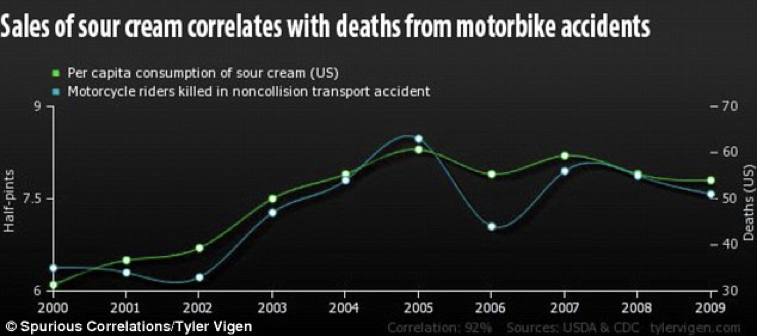
\includegraphics[width=0.9\linewidth]{_images/PannaAcida} 

}

\caption{Esempio di correlazione spuria}\label{fig:figName22}
\end{figure}

A volte il confounding non è casuale, ma è legato ad una variabile
esterna che si agisce all'insaputa dello sperimentatore. Ad esempio, è
stato osservato che il tasso di crimini è più alto nelle città che hanno
più chiese. La spiegazione di questo paradosso sta nel fatto che esiste
un `confounder', cioè l'ampiezza della popolazione. Nelle grandi città
si riscontrano sia una maggiore incidenza criminale, sia un grande
numero di chiese. In sostanza, la popolazione determina sia l'elevato
numero di chiese che l'elevato numero di crimini, ma queste ultime due
variabili non sono legate tra loro da una relazione causa-effetto (A
implica B e A implica C, ma B non implica C).

Il confounding non casuale è spesso difficile da evidenziare,
soprattutto se le correlazioni misurate sono spiegabili. Inoltre, non è
eliminabile con un'accurata randomizzazione, ma solo con l'esecuzione di
un esperimento totalmente controllato, nel quale ci si preoccupa di
rilevare tutte le variabili necessarie per spiegare gli effetti
riscontrati. Di questo è importante tener conto soprattutto negli
esperimenti osservazionali, dove il controllo è sempre più difficile e
meno completo.

\subsubsection{Pseudo-repliche e randomizzazione poco
attenta}\label{pseudo-repliche-e-randomizzazione-poco-attenta}

Per evidenziare questi problemi e comprendere meglio la differenza tra
un esperimento corretto e uno non corretto, è utilissima la
classificazione fatta da Hurlbert (1984), che riportiamo di seguito.

\begin{figure}

{\centering 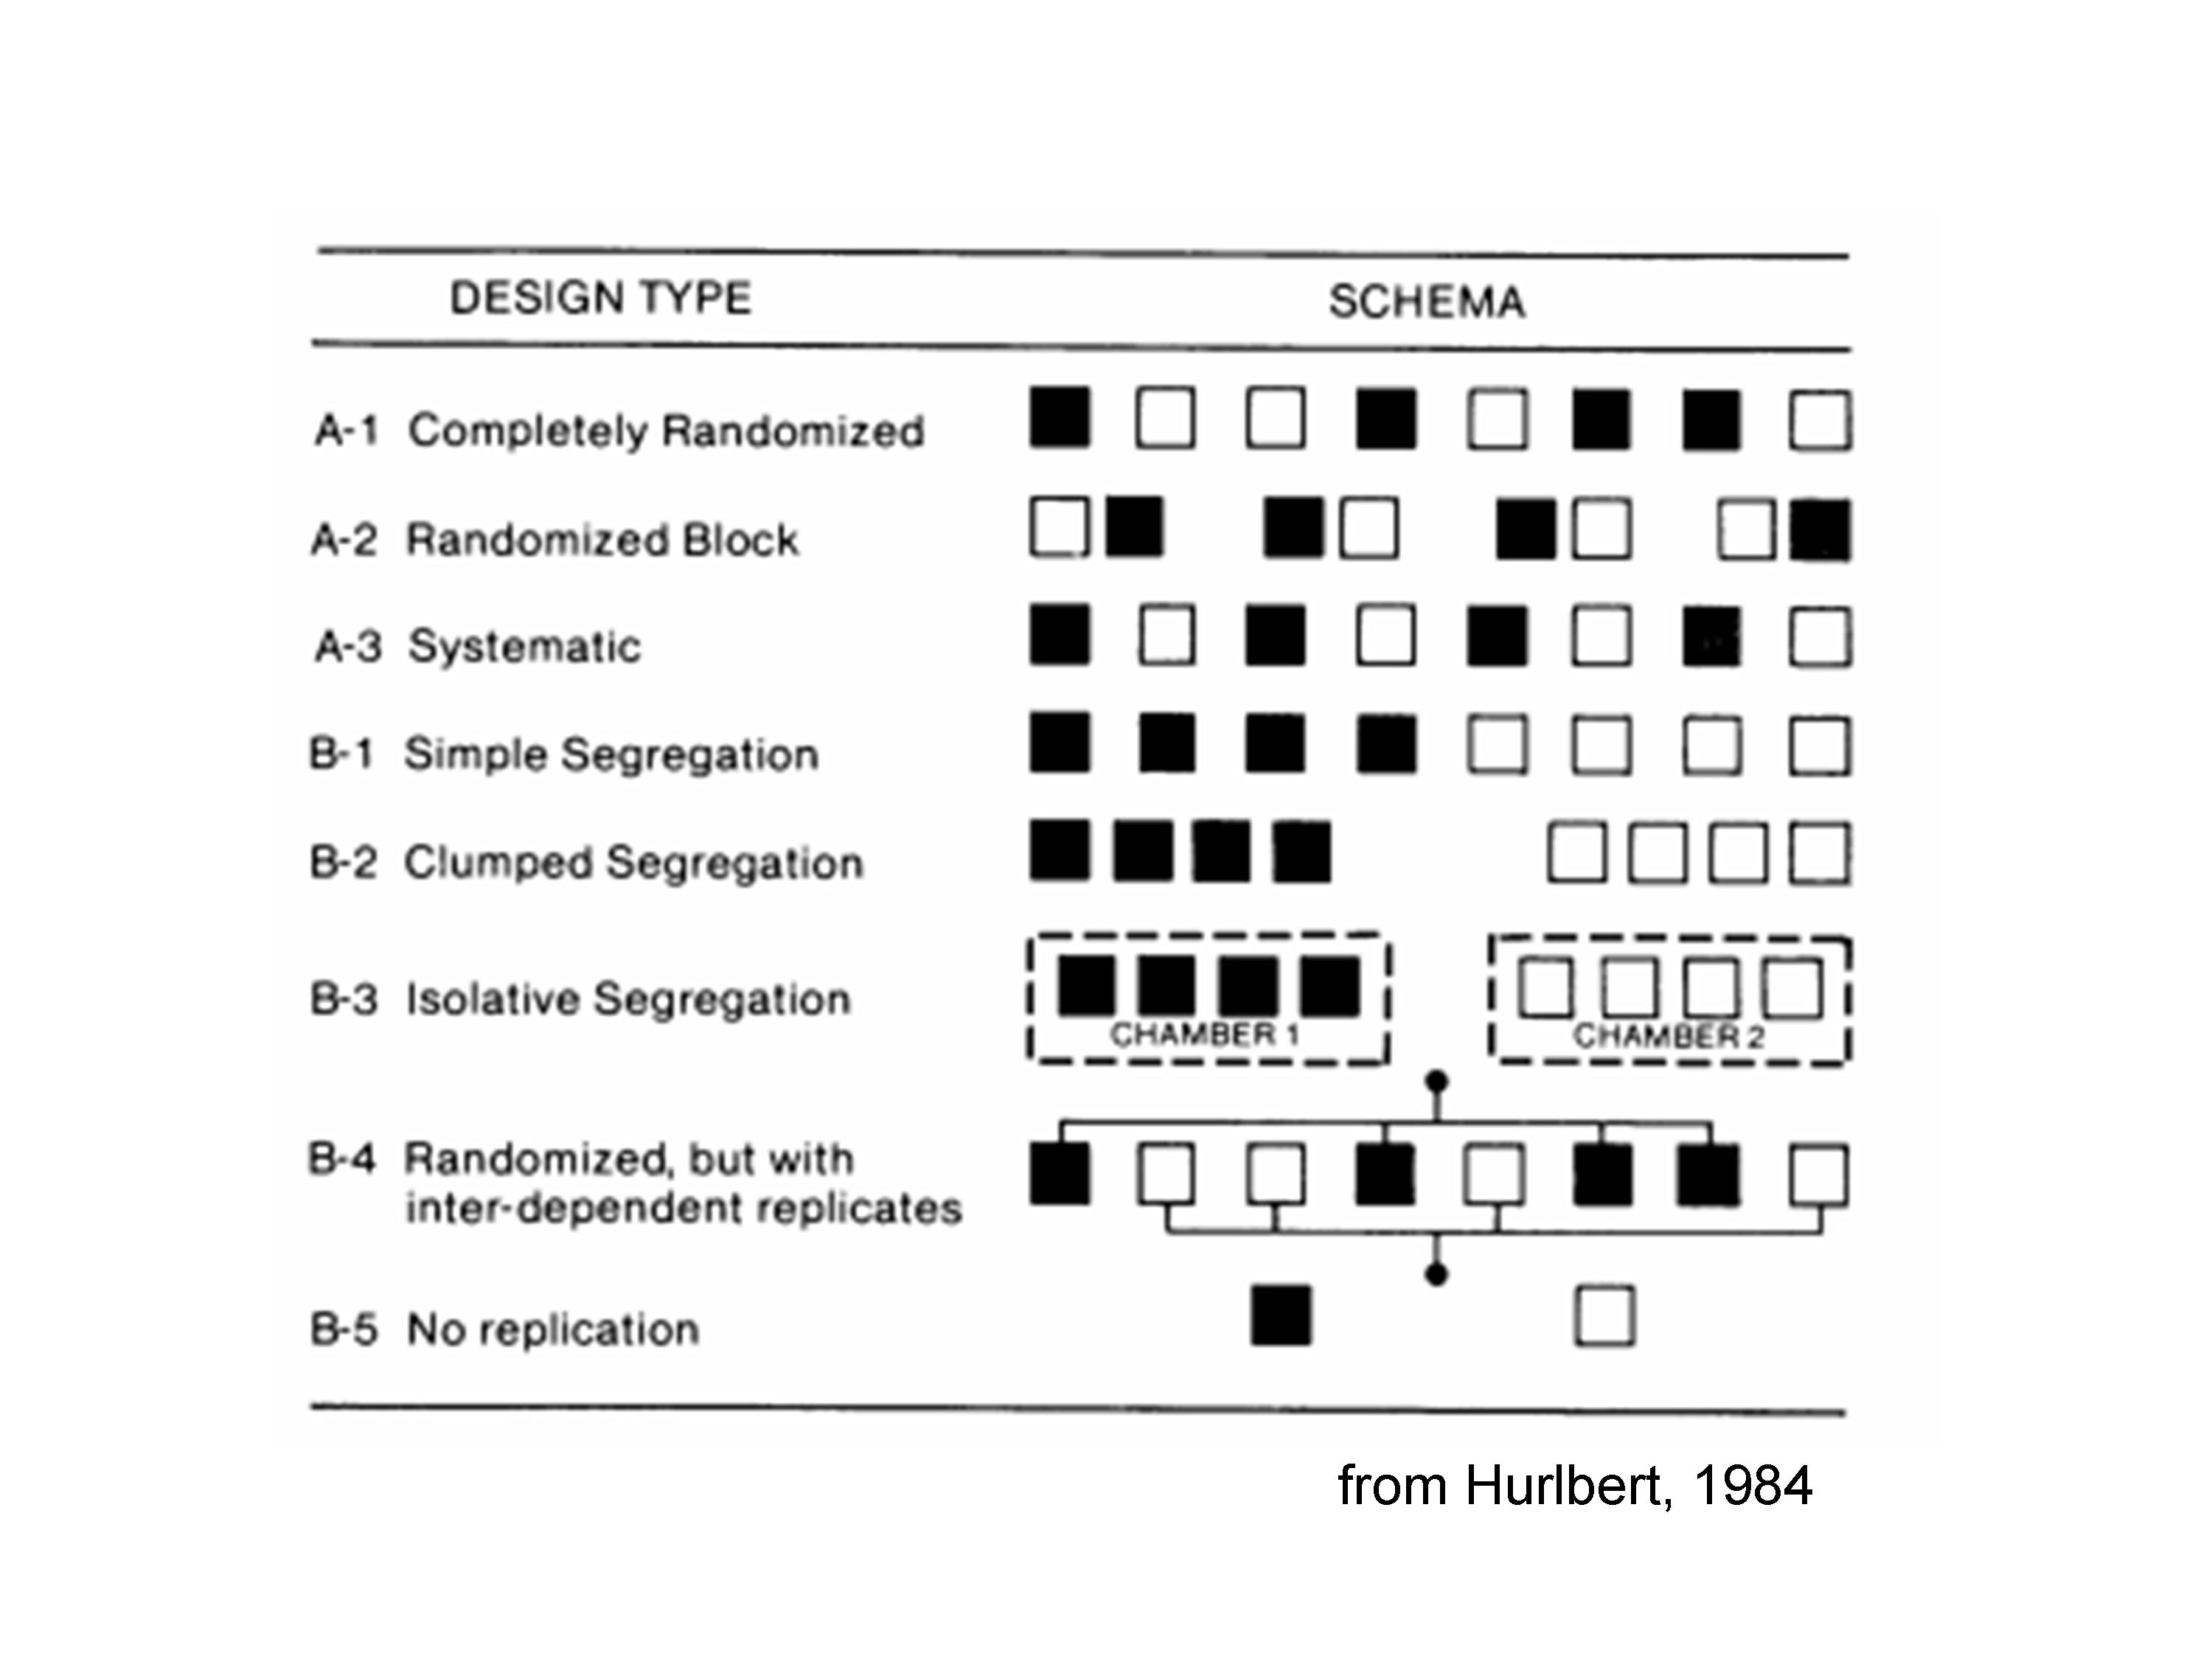
\includegraphics[width=0.9\linewidth]{_images/Randomisation} 

}

\caption{Indicazioni per una corretta randomizzazione (Hurlbert, 1984)}\label{fig:figName23}
\end{figure}

Vengono mostrati 8 soggetti, sottoposti a due trattamenti (bianco e
nero), con 8 disegni sperimentali diversi.

Il disegno A1 è corretto, in quanto si tratta di un esperimento
completamente randomizzato. Ugualmente, è valido il disegno A2, nel
quale le unità sperimentali sono state divise in quattro gruppi omogenei
e sono state trattate in modo randomizzato all'interno di ogni gruppo.

Il disegno A3 è quantomeno `sospetto': vi sono repliche vere, ma
l'allocazione dei trattamenti non è randomizzata ed avviene con un
processo sistematico per il quale `nero' e `bianco' si alternano. Cosa
succederebbe se vi fosse un gradiente di fertilità decrescente da destra
verso sinistra? Le unità nere sarebbero avvantaggiate rispetto alle
bianche! Insomma, rimangono sospetti di confounding, a meno che non si
sia assolutamente certi dell'assenza di gradienti, come capita ad
esempio se all'interno dei blocchi, dobbiamo creare una sequenza
spazio-temporale. Vediamo tre esempi:

\begin{enumerate}
\def\labelenumi{\arabic{enumi}.}
\tightlist
\item
  ho quattro piante e, per ogni pianta, voglio confrontare un ramo basso
  con uno alto: è evidente che i due trattamenti sono sempre ordinati in
  modo sistematico (basso prima di alto).
\item
  Dobbiamo valutare l'effetto di fitofarmaci somministrati in due epoche
  diverse (accestimento e inizio-levata); anche qui non possiamo
  randomizzare, giacché un'epoca precede sempre l'altra.
\item
  Dobbiamo confrontare la presenza di residui di un fitofarmaco a due
  profondità e non possiamo randomizzare, perché una profondità precede
  sempre l'altra nello spazio.
\end{enumerate}

In queste situazioni l'esperimento rimane valido, anche se la
randomizzazione segue un processo sistematico e non casuale.

Il disegno B1 è usualmente invalido: non vi è randomizzazione e ciò
massimizza i problemi del disegno A3: la separazione delle unità
sperimentali `bianche' e `nere' non consente una valutazione adeguata
dell'effetto del trattamento, che è confuso con ogni potenziale
differenza tra la parte destra e la sinistra dell'ambiente in cui la
sperimentazione viene eseguita. Ovviamente, la separazione può essere
non solo spaziale, ma anche temporale. Anche in questo caso diamo alcuni
esempi in cui una situazione come quella descritta in B1 è valida:

\begin{enumerate}
\def\labelenumi{\arabic{enumi}.}
\tightlist
\item
  Vogliamo confrontare la produzione in pianura e in collina. Ovviamente
  dobbiamo scegliere campioni in due situazioni fisicamente separate
\item
  Vogliamo confrontare la pescosità di due laghetti
\item
  Vogliamo confrontare la produttività di due campi contigui.
\end{enumerate}

Queste situazioni sono valide, anche se con una restrizione: non siamo
in grado di stabilire a chi debba essere attribuito l'effetto. Ad
esempio, per la prima situazione, pianura e collina possono dare
produzioni diverse per il suolo diverso, il clima diverso, la
precessione colturale diversa o un qualunque altro elemento che
differenzi le due località.

Il disegno B2 è analogo al disegno B1, ma il problema è più grave,
perché la separazione fisica è più evidente. Questo disegno è totalmente
sbagliato, a meno che non siamo specificatamente interessati all'effetto
località (vedi sopra).

Il disegno B3 è analogo al disegno B2, ma costituisce una situazione
molto frequente nella pratica scientifica. Immaginiamo infatti di voler
confrontare la germinazione dei semi a due temperature diverse,
utilizzando due camere climatiche e mettendo, in ognuna di esse, quattro
capsule Petri identiche. In questa situazione, l'effetto temperatura è
totalmente confuso con l'effetto `camera climatica (località)' e risente
di ogni malfunzionamento relativo ad una sola delle due camere. Inoltre,
le unità sperimentali con lo stesso trattamento di temperature non sono
manipolate in modo indipendente, dato che condividono la stessa camera
climatica. Di conseguenza, non si può parlare di repliche vere, bensì di
\textbf{pseudorepliche}.

Altri esempi di \textbf{pseudorepliche} sono schematizzati con il codice
B4. Ad esempio:

\begin{enumerate}
\def\labelenumi{\arabic{enumi}.}
\tightlist
\item
  trattare piante in vaso ed analizzare in modo indipendente i singoli
  individui invece che tutto il vaso;
\item
  trattare una parcella di terreno e prelevare da essa più campioni,
  analizzandoli separatamente;
\item
  trattare una capsula Petri ed analizzare separatamente i semi
  germinati al suo interno.
\end{enumerate}

Questi disegni, in assenza di repliche vere aggiuntive non sono da
considerarsi validi. Ad esempio, se io ho due vasetti trattati in modo
totalmente indipendente e da ciascuno di essi prelevo due piante e le
analizzo separatamente, il disegno è caratterizzato da due repliche vere
e due pseudorepliche per ogni replica ed è, pertanto, valido.

Il disegno B5 è invece evidentemente invalido, per totale mancanza di
repliche.

\section{Conclusione}\label{conclusione}

Disegnare un esperimento valido è un'arte e richiede profonda
attenzione; i principi fondamentali sono tre (controllo, replicazione e
randomizzazione) anche se declinarli non è sempre facile in tutti i
contesti di ricerca. Resta il fatto che nessuna informazione
scientificamente fondata può essere ottenuta da un esperimento che sia
invalido, per cattiva interpretazione di uno dei principi anzidetti.

\section{Per approfondimenti}\label{per-approfondimenti}

\begin{enumerate}
\def\labelenumi{\arabic{enumi}.}
\tightlist
\item
  Hurlbert, S., 1984. Pseudoreplication and the design of ecological
  experiments. Ecological Monographs, 54, 187-211
\item
  Kuehl, R. O., 2000. Design of experiments: statistical principles of
  research design and analysis. Duxbury Press (CHAPTER 1)
\end{enumerate}

\chapter{Progettare un esperimento}\label{progettare-un-esperimento}

Qualunque sia l'ambito scientifico, nella progettazione di un
esperimento possiamo individuare alcune fasi fondamentali, che proviamo
ad elencare:

\begin{enumerate}
\def\labelenumi{\arabic{enumi}.}
\tightlist
\item
  individuazione del background (ricerca bibliografica)
\item
  definizione dell'ipotesi scientifica;
\item
  definizione dell'obiettivo;
\item
  identificazione dei fattore/i sperimentale/i;
\item
  identificazione dei soggetti sperimentali e delle repliche;
\item
  identificazione delle variabili da rilevare;
\item
  allocazione randomizzata dei trattamenti (mappa dell'esperimento);
\item
  esecuzione dell'esperimento.
\end{enumerate}

Nell'analizzare questi aspetti, faremo riferimento ad alcuni esempi
pratici, che verranno presentati tra poco.

\section{\texorpdfstring{Ipotesi scientifica \(\rightarrow\) obiettivo
dell'esperimento}{Ipotesi scientifica \textbackslash{}rightarrow obiettivo dell'esperimento}}\label{ipotesi-scientifica-rightarrow-obiettivo-dellesperimento}

Trascurando la parte di ricerca bibliografica, che è pur fondamentale,
nel metodo scientifico galileiano, il punto di partenza di un
esperimento è l'\textbf{ipotesi scientifica}, che determina l'obiettivo
dell'esperimento. Si tratta del passaggio fondamentale dal quale dipende
in modo logico tutto il lavoro successivo. Gli obiettivi debbono essere:

\begin{enumerate}
\def\labelenumi{\arabic{enumi}.}
\tightlist
\item
  rilevanti
\item
  chiaramente definiti;
\item
  specifici;
\item
  misurabili;
\item
  raggiungibili/realistici;
\item
  temporalmente organizzati.
\end{enumerate}

Il rischio che si corre con obiettivi mal posti è quello di eseguire una
ricerca dispersiva, con raccolta di dati non necessari e/o mancanza di
dati fondamentali, con costi più elevati del necessario e un uso poco
efficiente delle risorse. In genere, prima si definisce un obiettivo
generale, seguito da uno o più obiettivi specifici, in genere proiettati
su un più breve spazio temporale e che possono essere visti anche come
le fasi necessarie per raggiungere l'obiettivo generale.

\section{Casi di studio - 1}\label{casi-di-studio---1}

Per meglio comprendere la situazione, poniamo cinque esempi pratici.

\subsection{Esempio 1 - Diserbo
chimico}\label{esempio-1---diserbo-chimico}

Si suppone che gli erbicidi A, B e C siano più efficaci di D, E ed F
verso \emph{Solanum nigrum}, una comune pianta infestante delle colture
di pomodoro. L'obiettivo generale della ricerca sarà quello di trovare
un'efficace soluzione per l'eliminazione di \emph{Solanum nigrum} dal
pomodoro. Gli obiettivi specifici saranno:

\begin{enumerate}
\def\labelenumi{\arabic{enumi}.}
\tightlist
\item
  valutare l'efficacia erbicida di A, B e C, confrontandola con quella
  di D, E ed F
\item
  valutare la selettività degli anzidetti erbicidi verso il pomodoro
\end{enumerate}

\subsection{Esempio 2 - Valutazione
varietale}\label{esempio-2---valutazione-varietale}

L'ipotesi è che le varietà di girasole A, B e C non abbiano la stessa
base genetica e quindi non siano tutte ugualmente produttive.
L'obiettivo generale è quello di capire quale tra A, B e C sia più
adatta alle condizioni pedoclimatiche della collina Umbra.

Gli obiettivi specifici sono quelli di valutare:

\begin{enumerate}
\def\labelenumi{\arabic{enumi}.}
\tightlist
\item
  produttività di A, B e C
\item
  stabilità produttiva di A, B e C
\end{enumerate}

\subsection{Esempio 3 - Diserbo
parziale}\label{esempio-3---diserbo-parziale}

Nella barbabietola da zucchero, il diserbo localizzato lungo la fila
consente di diminuire l'impiego di erbicidi. Tuttavia, se la coltura
precedente ha prodotto semi e se non abbiamo effettuato una lavorazione
profonda per interrarli, la coltura sarà più infestata e quindi sarà più
difficile ottenere una buona produttività con il diserbo parziale.

Su questa ipotesi costruiamo un esperimento volto a valutare
l'interazione tra lavorazione del terreno e diserbo chimico. Per
raggiungere questo obiettivo generale, proveremo a valutare se:

\begin{enumerate}
\def\labelenumi{\arabic{enumi}.}
\tightlist
\item
  il diserbo parziale consente di ottenere produzioni comparabili a
  quelle del diserbo totale
\item
  l'effetto erbicida è indipendente dalla lavorazione prescelta
\end{enumerate}

\subsection{Esempio 4 - Colture
poliennali}\label{esempio-4---colture-poliennali}

L'ipotesi scientifica è affine a quella dell'esempio 2, ma, in questo
caso, vogliamo porre a confronto tre varietà di erba medica (A, B e C).
La differenza sta nel fatto che l'erba medica è una coltura poliennale e
quindi vogliamo capire se il giudizio di merito è indipendente dall'anno
di coltivazione.

I nostri obiettivi specifici saranno quindi:

\begin{enumerate}
\def\labelenumi{\arabic{enumi}.}
\tightlist
\item
  valutare la produttività media delle varietà in prova
\item
  valutare le oscillazione nei quattro anni di durata del cotico erboso
\end{enumerate}

\subsection{Esempio 5 - Inquinamento da
micotossine}\label{esempio-5---inquinamento-da-micotossine}

Secondo le notizie in bibliografia, i datteri confezionati in vendita
nei supermercati contengono elevate quantità di micotossine. L'obiettivo
generale è quello di verificare il livello di infestazione e vedere se
questo cambia con il metodo di confezionamento.

\section{Identificazione dei fattori
sperimentali}\label{identificazione-dei-fattori-sperimentali}

Dopo aver definito l'obiettivo di un esperimento, è necessario chiarire
esattamente gli stimoli a cui saranno sottoposte le unità sperimentali.
Uno `stimolo' sperimentale prende il nome di \textbf{fattore
sperimentale}, che può avere più \textbf{livelli}. I livelli del fattore
sperimentale prendono il nome di \textbf{trattamenti (o tesi)
sperimentali}.

\section{Esperimenti
(multi)fattoriali}\label{esperimenti-multifattoriali}

In alcuni casi è necessario inserire in prova più di un fattore
sperimentale. In questo caso si parla di esperimenti
\textbf{fattoriali}, che possono essere \textbf{incrociati (crossed)}
quando sono presenti in prova tutte le possibili combinazioni dei
livelli di ogni fattore, oppure di esperimenti \textbf{innestati
(nested)} quando i livelli di un fattore cambiano al cambiare dei
livelli dell'altro.

Ad esempio:

\begin{enumerate}
\def\labelenumi{\arabic{enumi}.}
\tightlist
\item
  Immaginiamo di voler studiare due fattori sperimentali: la varietà di
  girasole (tre livelli: A, B e C) e la concimazione (2 livelli: pollino
  e urea). Abbiamo quindi 6 possibili trattamenti (combinazioni):
  A-pollina, A-urea, B-pollina, B-urea, C-pollina e C-urea. Il disegno è
  completamente incrociato.
\item
  Immaginiamo di voler confrontare due specie in agricoltura biologica
  (orzo e triticale), con tre varietà ciascuna (A, B e C per orzo, D, E
  e F per triticale). Anche in questo caso abbiamo sei trattamenti:
  orzo-A, orzo-B, orzo-C, triticale-D, triticale-E e triticale-F, ma il
  disegno è innestato, perché per il fattore sperimentale `varietà' i
  livelli cambiano a seconda dei livelli del fattore `specie'.
\end{enumerate}

\section{Aggiungere un controllo?}\label{aggiungere-un-controllo}

In alcuni casi si pone il problema di inserire in prova un trattamento
che funga da riferimento per tutti gli altri. In questi casi si parla
comunemente di \textbf{controllo} o \textbf{testimone}, che può essere

\begin{enumerate}
\def\labelenumi{\arabic{enumi}.}
\tightlist
\item
  non sottoposto a trattamento
\item
  trattato con placebo
\item
  trattato secondo le modalità usuali di riferimento
\end{enumerate}

\section{Fattori sperimentali di trattamento e di
blocco}\label{fattori-sperimentali-di-trattamento-e-di-blocco}

Finora abbiamo menzionato quelli che, in lingua inglese, vengono
definiti \emph{treatment factor} (trattamenti sperimentali). Tuttavia,
possono esserci altri fattori sperimentali non allocati, ma `innati' e
legati alla collocazione spazio-temporale o alle caratteristiche dei
soggetti. Questi fattori vengono definiti, sempre in inglese,
\emph{blocking factors}. Di questi fanno parte, ad esempio, il blocco,
la località ed ogni altro elemento che permette di raggruppare i
soggetti. Anche questi \emph{blocking factors} devono essere chiaramente
identificati ed elencati.

Su questa base identifichiamo i fattori sperimentali negli esempi
precedenti.

\section{Casi di studio - 2}\label{casi-di-studio---2}

\subsection{Esempio 1}\label{esempio-1}

Il fattore sperimentale oggetto di studio sarà il diserbo del pomodoro,
con 5 livelli inseriti in prova (6 trattamenti sperimentali): A, B, C,
D, E ed F. Inoltre, si ritiene opportuno inserire in prova un testimone
non trattato (NT), che ci permetterà di quantificare la percentuale di
malerbe controllate. Inoltre, sarà anche necessario inserire in prova un
testimone scerbato manualmente (ST), che ci permetterà di quantificare
eventuali perdite produttive dovute alla competizione residua o alla
fitotossicità del trattamento. In totale, avremo quindi 8 tesi
sperimentali. Come usuale in pieno campo, l'esperimento verrà disegnato
a blocchi randomizzati e sarà pertanto necessario inserire un fattore di
blocco.

\subsection{Esempio 2}\label{esempio-2}

Il fattore sperimentale in studio sarà la varietà di girasole con 3
livelli inclusi in prova (varietà A, B e C). Come testimone, inseriremo
la varietà di riferimento per la zona (D). Dato che eseguiremo questa
prova su un terreno nel quale vi sono due chiari gradienti di fertilità,
disegneremo l'esperimento considerando due fattori di blocco:
trasversale e longitudinale (spiego meglio tra poco\ldots{}). Poiché
dobbiamo valutare la stabilità produttiva, dovremo ripetere
l'esperimento più volte (es. in tre anni diversi) e quindi avremo un
secondo fattore sperimentale, incrociato con il primo.

\subsection{Esempio 3}\label{esempio-3}

In questo caso avremo due fattori sperimentali incrociati: il diserbo,
con due livelli (totale o parziale, localizzato sulla fila) e la
lavorazione, con tre livelli (aratura profonda, aratura superficiale e
\emph{minimum tillage}). Non vi è la necessità di un testimone, ma
avremo la necessità di un fattore di blocco. In totale, avremo sei tesi
sperimentali.

\subsection{Esempio 4}\label{esempio-4}

Il fattore sperimentale in studio sarà la varietà di erba medica con 3
livelli inclusi in prova (varietà A, B e C) ai quali aggiungiamo il
riferimento di zona (D) come testimone. Come nel caso del girasole,
dovremo valutare la stabilità produttiva negli anni, ma, dato che
abbiamo una coltura poliennale, non avremo bisogno di ripetere la prova,
ma potremo ripetere le osservazioni per quattro anni sulla stessa prova.

\subsection{Esempio 5}\label{esempio-5}

Per questo esperimento vengono considerate tre diverse modalità di
confezionamento (carta, busta di plastica, scatola di plastica
perforata). Non vi è necessità di un testimone, ma, dato che le diverse
confezioni verranno acquistate in diversi supermercati e dato che
sospettiamo differenze nella conservazione tra un supermercato e
l'altro, utilizzeremo il supermercato come fattore di raggruppamento.

\section{Identificazione delle unità sperimentali e delle
repliche}\label{identificazione-delle-unita-sperimentali-e-delle-repliche}

\subsection{Cornice di campionamento e numero di
repliche}\label{cornice-di-campionamento-e-numero-di-repliche}

Per i primi quattro esempi verranno eseguite prove di pieno campo, nella
Media Valle del Tevere, che rappresenta la cornice di campionamento
adeguata per l'obiettivo previsto. Sappiamo di dover selezionare
appezzamenti di terreno

\begin{enumerate}
\def\labelenumi{\arabic{enumi}.}
\tightlist
\item
  rappresentativi della Media Valle del Tevere,
\item
  omogenei.
\end{enumerate}

L'omogeneità dell'ambiente è fondamentale per aumentare la precisione
dell'esperimento. La scelta dell'appezzamento è chiaramente fondamentale
ed è guidata dall'esperienza, tenendo conto anche di aspetti come la
facilità di accesso e la vicinanza di strutture (laboratori,
capannoni\ldots{}) che consentano un'accurata esecuzione degli eventuali
prelievi.

Oltre alla scelta dell'appezzamento, si possono anche utilizzare alcune
strategie per favorire una buona omogeneità delle parcelle. Spesso si
usa far precedere la prova da una coltura di `omogeneizzazione', ad
esempio avena, che è molto avida di azoto e lascia nel terreno poca
fertilità residua. Oppure un prato di erba medica, che, grazie agli
sfalci periodici, lascia il terreno libero da piante infestanti.

Trattandosi di esperimenti di campo, il numero di repliche sarà quattro,
per ogni trattamento e l'unità sperimentale sarà una parcella, della
quale dovremo valutare forma e dimensioni.

Per il quinto esempio, la cornice di campionamento sarà data dal
territorio del comune di Perugia. L'unità sperimentale sarà la
confezione e la scelta del numero di repliche dovrà essere compatibile
con la capacità di analisi per la determinazione dell'inquinamento da
micotossine. E' ragionevole pensare che 30 repliche (90 confezioni
totali) possano essere adeguate per rappresentatività e facilità di
gestione.

\subsection{Campionamento delle unità
sperimentali}\label{campionamento-delle-unita-sperimentali}

Per le quattro prove di pieno campo, una volta scelto l'appezzamento,
dovremo campionare le parcelle di terreno. Questa operazione viene
usualmente eseguita su carta, redigendo la \textbf{mappa
dell'esperimento}. In primo luogo, si decide la \textbf{dimensione e la
forma della parcella}.

L'aspetto fondamentale è che ogni parcella deve contenere un numero di
piante sufficientemente alto da essere rappresentativo. Per questo
motivo le colture a bassa fittezza hanno sempre bisogno di parcelle più
grandi che non quelle ad alta fittezza. La dimensione non deve tuttavia
eccedere una certa soglia, in quanto con essa aumenta anche la
variabilità del terreno e, di conseguenza, diminuisce l'omogeneità
dell'esperimento. Per questo motivo, talvolta si preferisce diminuire la
dimensione delle parcelle ed, avendo lo spazio sufficiente, aumentare il
numero delle repliche.

Nello stabilire la dimensione delle parcelle, dovremo tener conto del
fatto che la parte più delicata è il bordo, in quanto le piante che si
trovano lungo il bordo esterno risentono di condizioni diverse dalle
altre piante situate al centro della parcella (\textbf{effetto bordo}).
Questo determina variabilità all'interno della parcella, che possiamo
minimizzare raccogliendo solo la parte centrale. Si viene così a
distinguere la superficie totale della parcella dalla superficie di
raccolta (\textbf{superficie utile}), che può essere anche molto minore
di quella totale.

In generale si ritiene che le colture ad elevata fittezza (frumento,
cereali, erba medica\ldots{}) dovrebbero avere parcelle di almeno 10-20
m\(^2\), mentre a bassa fittezza (mis, girasole\ldots{}) dovrebbero
avere parcelle di almeno 20-40 m\(^2\). Queste dimensioni sono riferite
alla superficie utile di raccolta, non alla dimensione totale.

Per quanto riguarda la forma, le parcelle quadrate minimizzano l'effetto
bordo, perché, a parità di superficie, hanno un perimetro più basso.
Tuttavia esse sono di più difficile gestione, in quanto, considerando il
fronte di lavoro di una seminatrice o una mietitrebbiatrice parcellare,
possono richiedere la semina o la raccolta in più passate, il che
finisce per essere una fonte di errore. Per questo motivo le parcelle
sono usualmente rettangolari, con una larghezza pari a quella della
macchina impiegata per la semina.

Di conseguenza, per i quattro esempi in studio potremmo utilizzare una
dimensione delle parcelle di 20 m\(^2\) per l'erba medica (2 m di
larghezza per 10 m di lunghezza) e di 22.5 m\(^2\) per pomodoro, mais e
barbabietola da zucchero (2.25 m di larghezza per 10 metri di
lunghezza).

A questo punto possiamo redigere la mappa per il primo esempio. Dato che
il campo di prova è largo 30 metri e lungo 400 metri, potremmo
immaginare di disegnare otto file di parcelle in senso trasversale (8 x
2.25 m = 18 m), di modo che l'esperimento non sia troppo lungo (il che
ne aumenterebbe la variabilità), ma rimanga spazio sufficiente ai lati,
per evitare di avvicinarsi troppo alle scoline, dove possono
manifestarsi ristagni idrici.

La mappa dell'esperimento è un elemento fondamentale e deve riportare
tutte le informazioni relative al disegno sperimentale. E' anche
importante indicare la direzione del Nord, in modo da facilitare
l'orientamento della mappa stessa. Notare inoltre che, intorno alla
prova, abbiamo sistemato altre parcelle fuori esperimento con funzione
di `bordi'. In questo modo si evita che i bordi esterni delle parcelle
esterne siano esposti a condizioni molto diverse dagli altri, cosa che
potrebbe accentuare l'effetto `bordo', di cui abbiamo parlato in
precedenza. Queste parcelle di bordo verranno trattate in modo ordinario
(semina e diserbo tradizionale del pomodoro).

\begin{figure}

{\centering 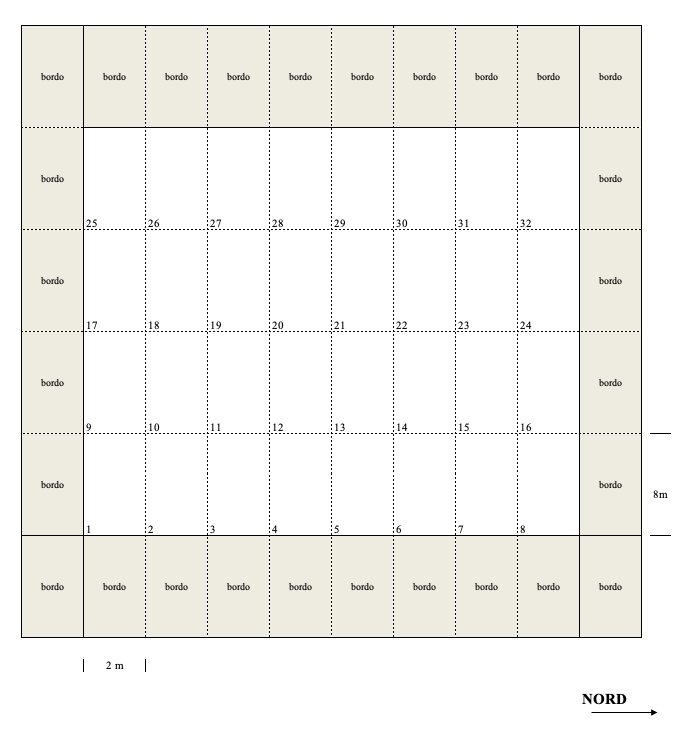
\includegraphics[width=0.9\linewidth]{_images/Mappa1} 

}

\caption{Mappa dell'esperimento relativo all esempio 1}\label{fig:figName31}
\end{figure}

Per l'esperimento relativo all'esempio 5, l'unità sperimentale è una
singola confezione di datteri, con le tipologie previste dal piano.

\begin{figure}

{\centering 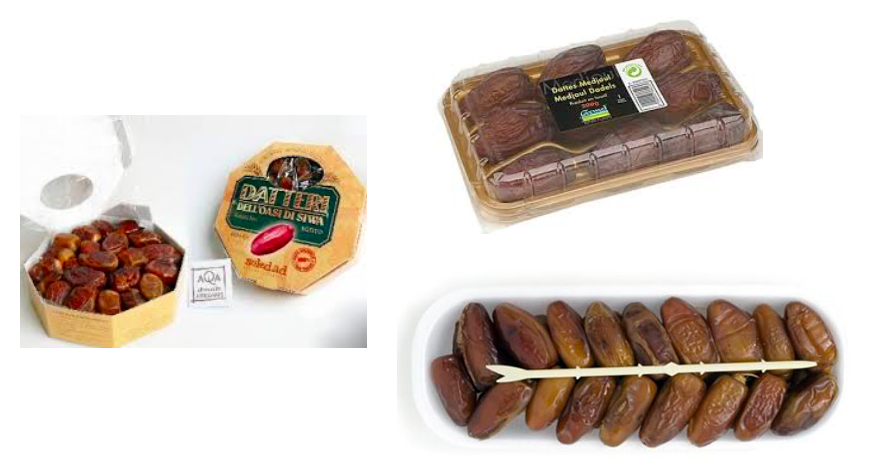
\includegraphics[width=0.9\linewidth]{_images/Datteri} 

}

\caption{Tipologie delle confezioni di datteri}\label{fig:figName32}
\end{figure}

Siccome è abbastanza scomodo campionare confezioni di datteri
casualmente all'interno del Comune di Perugia, si preferisce un
campionamento `stratificato', selezionando 10 supermercati
rappresentativi, nelle zone più densamente popolate della città.
All'interno di ogni supermercato, si selezioneranno casualmente tre
repliche per ogni tipo di confezione.

\section{Scelta delle variabili da
rilevare}\label{scelta-delle-variabili-da-rilevare}

Durate e al termine dell'esperimento, sarà necessario rilevare le più
importanti caratteristiche dei soggetti sperimentali, sia quelle innate,
sia quelle indotte dai trattamenti sperimentali. Per ogni singolo
carattere, l'insieme delle modalità/valori che ognuno dei soggetti
presenta prende il nome di \textbf{variabile} (proprio perché varia,
cioè assume diversi valori, a seconda del soggetto). Ad esempio, quando
stiamo studiando l'effetto di due diserbanti su piante infestanti
appartenenti ad una certa specie, posto che l'unità sperimentale è
costituita da una singola pianta, possiamo avere le seguenti variabili:
il prodotto diserbante con cui ogni pianta è stata trattata, il peso di
ogni pianta prima del trattamento, il peso di ogni pianta dopo il
trattamento.

Le variabili sperimentali possono essere molto diverse tra di loro ed è
piuttosto importante saperle riconoscere, perché questo condiziona il
tipo di analisi statistica da eseguire.

\subsection{Variabili nominali
(categoriche)}\label{variabili-nominali-categoriche}

Le variabili nominali esprimono, per ciascun soggetto, l'appartenenza ad
una determinata categoria o raggruppamento. L'unica caratteristica delle
categorie è l'esclusività, cioè un soggetto che appartiene ad una di
esse non può appartenere a nessuna delle altre. Variabili nominali sono,
ad esempio, il sesso, la varietà, il tipo di diserbante impiegato, la
modalità di lavorazione e così via. Le variabili categoriche permettono
di raggruppare i soggetti, ma non possono essere utilizzate per fare
calcoli, se non per definire le proporzioni dei soggetti in ciascun
gruppo.

\subsection{Variabili ordinali}\label{variabili-ordinali}

Anche le variabili ordinali esprimono, per ciascun soggetto,
l'appartenenza ad una determinata categoria o raggruppamento. Tuttavia,
le diverse categorie sono caratterizzate, oltre che dall'esclusività,
anche da una relazione di ordine, nel senso che è possibile stabilire
una naturale graduatoria tra esse. Ad esempio, la risposta degli
agricoltori a domande relative alla loro percezione sull'utilità di una
pratica agronomica può essere espressa utilizzando una scala con sei
categorie (0, 1, 2, 3, 4 e 5), in ordine crescente da 0 a 5 (scala
Likert). Di conseguenza possiamo confrontare categorie diverse ed
esprimere un giudizio di ordine (2 è maggiore di 1, 3 è minore di 5), ma
non possiamo eseguire operazioni matematiche, tipo sottrarre dalla
categoria 3 la categoria 2 e così via, dato che la distanza tra le
categorie non è necessariamente la stessa.

\subsection{Variabili quantitative
discrete}\label{variabili-quantitative-discrete}

Le variabili discrete sono caratterizzate dal fatto che possiedono,
oltre alle proprietà dell'esclusività e dell'ordine, anche quella
dell'equidistanza tra gli attributi (es., in una scala a 5 punti, la
distanza -- o la differenza -- fra 1 e 3 è uguale a quella fra 2 e 4 e
doppia di quella tra 1 e 2). Una tipica variabile discreta è il
conteggio di piante infestanti all'interno di una parcella di terreno.

Le variabili discrete consentono la gran parte delle operazioni
matematiche e permettono di calcolare molte importanti statistiche come
la media, la mediana, la varianza e la deviazione standard.

\subsection{Variabili quantitative
continue}\label{variabili-quantitative-continue}

Le variabili quantitative continue possiedono tutte le proprietà
precedentemente esposte (esclusività delle categorie, ordine, distanza)
oltre alla continuità, almeno in un certo intervallo. Tipiche variabili
continue sono l'altezza, la produzione, il tempo, la fittezza\ldots{}

Dato che gli strumenti di misura nella realtà sono caratterizzati da una
certa risoluzione, si potrebbe arguire che misure su scala continua
effettivamente non esistono. Tuttavia questo argomento è più teorico che
pratico e, nella ricerca biologica, consideriamo continue tutte le
misure nelle quali la risoluzione dello strumento è sufficientemente
piccola rispetto alla grandezza da misurare. Viceversa, le variabili
continue sono piuttosto rare nelle scienze economiche e sociali in
genere.

La quantità di informazione fornita dagli strumenti di valutazione
cresce passando dalle scale nominali, di più basso livello, a quelle
quantitative continue, di livello più elevato. Variabili esprimibili con
scale quantitative continue o discrete possono essere espresse anche con
scale qualitative, adottando un'opportuna operazione di classamento. Il
contrario, cioè trasformare in quantitativa una variabile qualitativa,
non è invece possibile.

\subsection{Rilievi visivi e
sensoriali}\label{rilievi-visivi-e-sensoriali}

Nella pratica sperimentale è molto frequente l'adozione di metodi di
rilievo basati sull'osservazione di un fenomeno attraverso uno dei sensi
(più spesso, la vista, ma anche gusto e olfatto) e l'assegnazione di una
valutazione su scala categorica, ordinale o, con un po' di prudenza,
quantitativa discreta o continua. Ad esempio, il ricoprimento delle
piante infestanti, la percentuale di controllo di un erbicida e la sua
fitotossicità vengono spesso rilevati visivamente, su scale da 0 a 100 o
simili.

I vantaggi di questa tecnica sono molteplici:

\begin{enumerate}
\def\labelenumi{\arabic{enumi}.}
\tightlist
\item
  Basso costo ed elevata velocità
\item
  Possibilità di tener conto di alcuni fattori perturbativi esterni, che
  sono esclusi dalla valutazione, contrariamente a quello che succede
  con metodi oggettivi di misura
\item
  non richiede strumentazione costosa
\end{enumerate}

A questi vantaggi fanno da contraltare alcuni svantaggi, cioè:

\begin{enumerate}
\def\labelenumi{\arabic{enumi}.}
\tightlist
\item
  Minor precisione (in generale)
\item
  Soggettività
\item
  L'osservatore può essere prevenuto
\item
  Difficoltà di mantenere uniformità di giudizio
\item
  Richiede esperienza specifica e allenamento
\end{enumerate}

I rilievi sensoriali sono ben accettati nella pratica scientifica in
alcuni ambiti ben definiti, anche se richiedono attenzione nell'analisi
dei dati non potendo essere assimilati \emph{tout court} con le misure
oggettive su scala continua.

\subsection{Variabili di
confondimento}\label{variabili-di-confondimento}

Quando si pianificano i rilievi da eseguire, oppure anche nel corso
dell'esecuzione di un esperimento, bisogna tener presente non soltanto
la variabile che esprime l'effetto del trattamento, ma anche tutte le
variabili che misurano possibili fattori di confondimento.

Ad esempio, immaginiamo di voler valutare la produttività di una specie
arborea in funzione della varietà. Immaginiamo anche di sapere che, per
questa specie, la produttività dipende anche dall'età. Se facciamo un
esperimento possiamo utilizzare alberi della stessa età per minimizzare
la variabilità dei soggetti. Tuttavia, se questo non fosse possibile,
per ogni albero dobbiamo rilevare non solo la produttività, ma anche
l'età, in modo da poter valutare anche l'effetto di questo fattore
aggiuntivo e separarlo dall'effetto della varietà. In questo modo
l'esperimento diviene molto più preciso.

\section{Casi di studio - 3}\label{casi-di-studio---3}

Per gli esempi in studio, immaginiamo per semplicità di dover rilevare
la produzione per gli esempi da 1 a 4 e il contenuto di micotossine per
l'esempio 5. Inoltre, per l'esempio 2, immaginiamo di dover rilevare
anche il peso di mille semi. Per questo, prenderemo dalla produzione di
granella di ogni parcella, quattro sub-campioni da mille semi, da
sottoporre a successive misure.

\section{Allocazione dei trattamenti}\label{allocazione-dei-trattamenti}

Il problema dell'allocazione dei trattamenti non si pone con l'esempio
5, in quanto, trattandosi di un esperimento osservazionale, le
confezione sono già `naturalmente' trattate, cioè appartengono già,
all'atto del campionamento, alla tipologia di confezionamento prescelta.

Per tutti gli esperimenti disegnati si pone invece il problema di
scegliere quali soggetti trattare e con cosa. Per i nostri esempi
(escluso il 5), abbiamo già redatto la mappa delle parcelle, secondo le
necessità. A questo punto dobbiamo assegnare ad ogni parcella il suo
trattamento, assicurando il numero di repliche prescelto. Gli schemi
sperimentali di seguito descritti sono quelli più comunemente usati
nella sperimentazione di pieno campo (LeClerg, Leonard, and Clark
\protect\hyperlink{ref-leclerg1962_FieldPlotTechnique}{1962}), ma, con
le opportune modifiche, possono trovare impiego anche in molte altre
discipline scientifiche.

Negli esperimenti più semplici lo schema sperimentale può essere
pianificato a mano. Per esperimenti complessi potremo invece utilizzare
il computer; in R, potremo utilizzare, ad esempio, il package
\emph{agricolae} (de Mendiburu
\protect\hyperlink{ref-de-Mendiburu:2019aa}{2019}), seguento il codice
che troverete nei paragrafi seguenti.

\section{Casi di studio - 4}\label{casi-di-studio---4}

\subsection{Esempio 1}\label{esempio-1-1}

Questo esempio va disegnato a blocchi randomizzati; tuttavia, a titolo
di esempio, esamineremo anche la possibilità che venga disegnato a
randomizzazione completa. Quest'ultimo disegno è il più semplice e
consiste nell'assegnare ogni trattamento a quattro parcelle casualmente
scelte. Con R bisognerà prima creare il vettore dei nomi delle tesi e il
numero di repliche per tesi

\begin{Shaded}
\begin{Highlighting}[]
\KeywordTok{library}\NormalTok{(agricolae)}
\NormalTok{trt <-}\StringTok{ }\KeywordTok{c}\NormalTok{(}\StringTok{"A"}\NormalTok{, }\StringTok{"B"}\NormalTok{, }\StringTok{"C"}\NormalTok{, }\StringTok{"D"}\NormalTok{, }\StringTok{"E"}\NormalTok{, }\StringTok{"F"}\NormalTok{, }\StringTok{"NT"}\NormalTok{, }\StringTok{"TS"}\NormalTok{)}
\NormalTok{reps <-}\StringTok{ }\KeywordTok{rep}\NormalTok{(}\DecValTok{4}\NormalTok{, }\DecValTok{8}\NormalTok{)}
\NormalTok{design <-}\StringTok{ }\KeywordTok{design.crd}\NormalTok{(trt, }\DataTypeTok{r=}\NormalTok{reps, }\DataTypeTok{seed=}\DecValTok{777}\NormalTok{, }\DataTypeTok{serie=}\DecValTok{0}\NormalTok{)}
\NormalTok{design}\OperatorTok{$}\NormalTok{book}
\NormalTok{##    plots r trt}
\NormalTok{## 1      1 1   E}
\NormalTok{## 2      2 1   C}
\NormalTok{## 3      3 1   B}
\NormalTok{## 4      4 2   C}
\NormalTok{## 5      5 1   F}
\NormalTok{## 6      6 1  TS}
\NormalTok{## 7      7 1  NT}
\NormalTok{## 8      8 1   D}
\NormalTok{## 9      9 2  NT}
\NormalTok{## 10    10 1   A}
\NormalTok{## 11    11 2  TS}
\NormalTok{## 12    12 2   F}
\NormalTok{## 13    13 3  NT}
\NormalTok{## 14    14 3   C}
\NormalTok{## 15    15 3  TS}
\NormalTok{## 16    16 2   D}
\NormalTok{## 17    17 3   D}
\NormalTok{## 18    18 2   E}
\NormalTok{## 19    19 3   E}
\NormalTok{## 20    20 4  NT}
\NormalTok{## 21    21 2   A}
\NormalTok{## 22    22 4   D}
\NormalTok{## 23    23 4   E}
\NormalTok{## 24    24 3   A}
\NormalTok{## 25    25 4   C}
\NormalTok{## 26    26 2   B}
\NormalTok{## 27    27 4   A}
\NormalTok{## 28    28 3   F}
\NormalTok{## 29    29 3   B}
\NormalTok{## 30    30 4  TS}
\NormalTok{## 31    31 4   F}
\NormalTok{## 32    32 4   B}
\end{Highlighting}
\end{Shaded}

Possiamo ora riportare la randomizzazione sulla mappa disegnata in
precedenza.

\begin{figure}

{\centering 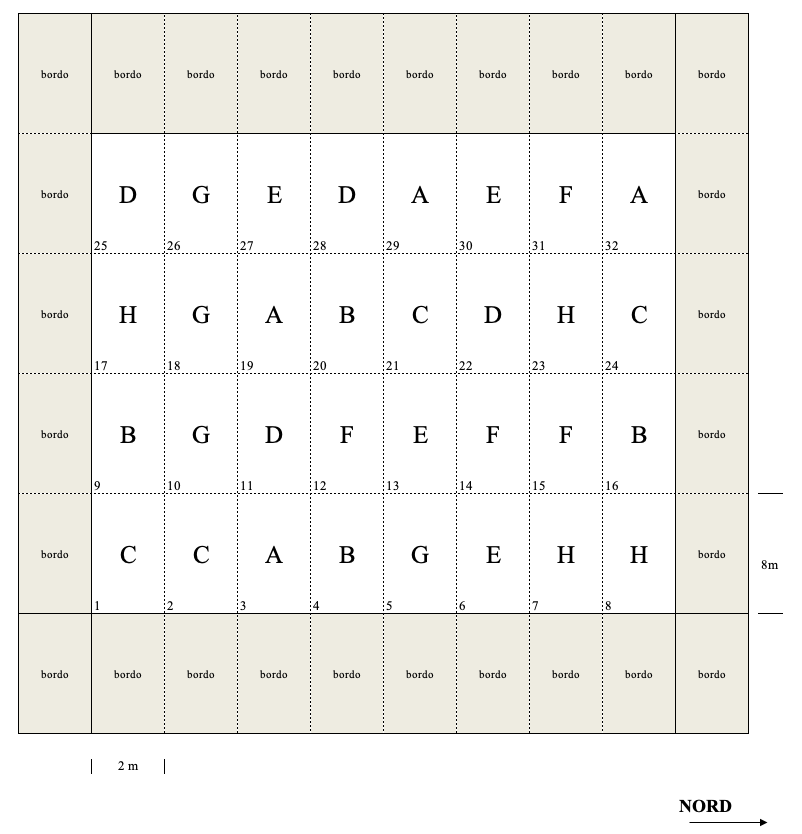
\includegraphics[width=0.9\linewidth]{_images/Mappa1CRD} 

}

\caption{Schema sperimentale a randomizzazione completa per l'Esempio 1}\label{fig:figName33}
\end{figure}

Questo schema è eccellente se l'ambiente è molto uniforme. Tuttavia, nel
caso di un esperimento di campo è lecito aspettarsi un gradiente
trasversale, dato che il campo sarà certamente meno fertile vicino alle
scoline. Per questo motivo disegneremo l'esperimento a blocchi
randomizzati, dividendo prima l'appezzamento in quattro blocchi
perpendicolari al gradiente di fertilità. Ad esempio il blocco 1
conterrà le parcelle 1, 9, 17, 25, 2, 10, 18 e 26, cioè le prime due
colonne della mappa, con un numero di parcelle esattamente uguali al
numero delle tesi. Il blocco 2 conterrà le colonne 3 e 4 e così via.
Dato che il gradiente è trasversale, le parcelle di un stesso blocco
saranno più omogenee che non parcelle su blocchi diversi. Dopo aver
diviso la mappa in quattro blocchi di otto parcelle, possiamo allocare
gli otto trattamenti a random all'interno di ogni blocco. Con R è
possibile utilizzare il codice seguente (notare che la numerazione
assegnata da R è diversa dalla nostra, anche se possiamo far riferimento
ai valori crescenti all'interno di ogni blocco).

\begin{Shaded}
\begin{Highlighting}[]
\NormalTok{reps <-}\StringTok{ }\DecValTok{4}
\NormalTok{designRCBD <-}\StringTok{ }\KeywordTok{design.rcbd}\NormalTok{(trt, }\DataTypeTok{r=}\NormalTok{reps, }\DataTypeTok{seed=}\DecValTok{777}\NormalTok{, }\DataTypeTok{serie=}\DecValTok{2}\NormalTok{)}
\NormalTok{book2 <-}\StringTok{ }\NormalTok{designRCBD}\OperatorTok{$}\NormalTok{book}
\NormalTok{book2}
\NormalTok{##    plots block trt}
\NormalTok{## 1    101     1   E}
\NormalTok{## 2    102     1   B}
\NormalTok{## 3    103     1  NT}
\NormalTok{## 4    104     1   F}
\NormalTok{## 5    105     1   D}
\NormalTok{## 6    106     1  TS}
\NormalTok{## 7    107     1   C}
\NormalTok{## 8    108     1   A}
\NormalTok{## 9    201     2   F}
\NormalTok{## 10   202     2   A}
\NormalTok{## 11   203     2   C}
\NormalTok{## 12   204     2   E}
\NormalTok{## 13   205     2  TS}
\NormalTok{## 14   206     2   B}
\NormalTok{## 15   207     2  NT}
\NormalTok{## 16   208     2   D}
\NormalTok{## 17   301     3  TS}
\NormalTok{## 18   302     3  NT}
\NormalTok{## 19   303     3   F}
\NormalTok{## 20   304     3   A}
\NormalTok{## 21   305     3   B}
\NormalTok{## 22   306     3   E}
\NormalTok{## 23   307     3   C}
\NormalTok{## 24   308     3   D}
\NormalTok{## 25   401     4   D}
\NormalTok{## 26   402     4  TS}
\NormalTok{## 27   403     4   A}
\NormalTok{## 28   404     4   F}
\NormalTok{## 29   405     4   E}
\NormalTok{## 30   406     4   C}
\NormalTok{## 31   407     4   B}
\NormalTok{## 32   408     4  NT}
\end{Highlighting}
\end{Shaded}

Anche in questo caso, riportiamo tutto sulla mappa.

\begin{figure}

{\centering 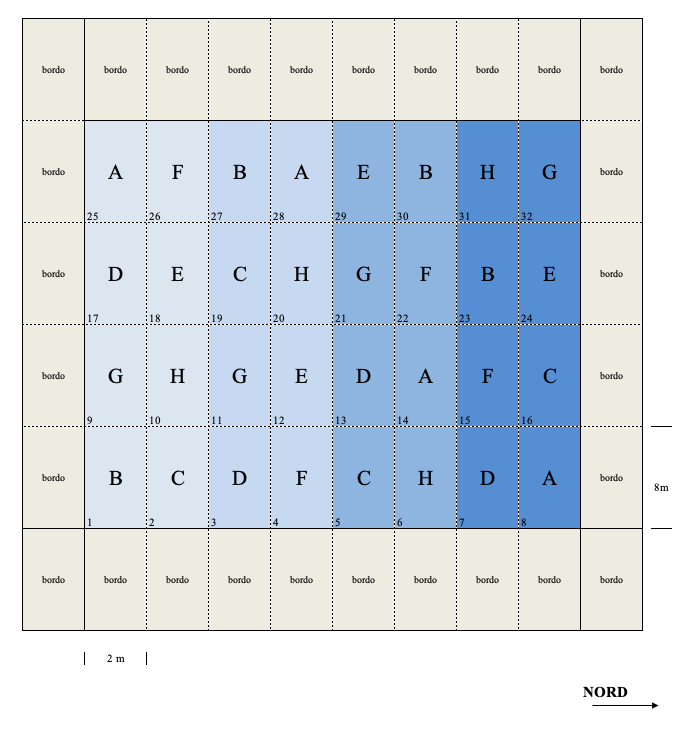
\includegraphics[width=0.9\linewidth]{_images/Mappa1CRBD} 

}

\caption{Schema sperimentale a blocchi randomizzati per l'Esempio 1}\label{fig:figName34}
\end{figure}

\subsection{Esempio 2}\label{esempio-2-1}

In questo caso, per ognuno dei tre anni di prova, la mappa contiene una
griglia 4 x 4, analoga a quella dell'esperimento precedente, ma più
piccola. Nella mappa potremo quindi identificare, esclusi i bordi,
quattro colonne e quattro righe. Dato che abbiamo presupposto
l'esistenza di un gradiente trasversale e lungitudinale (tra righe e tra
colonne), l'allocazione dei trattamenti dovrà esser fatta in modo che
ognuno di essi si trovi su ogni riga e ogni colonna. Questo tipo di
disegno prende il nome di \textbf{Quadrato latino}.

Anche in questo caso potremo chiedere ad R di aiutarci a trovare la
combinazione corretta (anche se questo potrebbe essere comodamente fatto
a mano).

\begin{Shaded}
\begin{Highlighting}[]
\NormalTok{trt <-}\StringTok{ }\KeywordTok{c}\NormalTok{(}\StringTok{"A"}\NormalTok{, }\StringTok{"B"}\NormalTok{, }\StringTok{"C"}\NormalTok{, }\StringTok{"D"}\NormalTok{)}
\NormalTok{designLS <-}\StringTok{ }\KeywordTok{design.lsd}\NormalTok{(trt, }\DataTypeTok{seed=}\DecValTok{543}\NormalTok{, }\DataTypeTok{serie=}\DecValTok{2}\NormalTok{)}
\NormalTok{designLS}\OperatorTok{$}\NormalTok{book}
\NormalTok{##    plots row col trt}
\NormalTok{## 1    101   1   1   C}
\NormalTok{## 2    102   1   2   A}
\NormalTok{## 3    103   1   3   B}
\NormalTok{## 4    104   1   4   D}
\NormalTok{## 5    201   2   1   D}
\NormalTok{## 6    202   2   2   B}
\NormalTok{## 7    203   2   3   C}
\NormalTok{## 8    204   2   4   A}
\NormalTok{## 9    301   3   1   B}
\NormalTok{## 10   302   3   2   D}
\NormalTok{## 11   303   3   3   A}
\NormalTok{## 12   304   3   4   C}
\NormalTok{## 13   401   4   1   A}
\NormalTok{## 14   402   4   2   C}
\NormalTok{## 15   403   4   3   D}
\NormalTok{## 16   404   4   4   B}
\end{Highlighting}
\end{Shaded}

\begin{figure}

{\centering 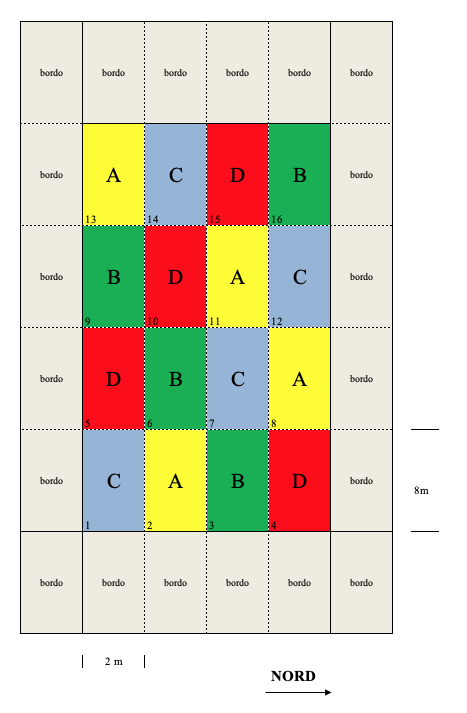
\includegraphics[width=0.65\linewidth]{_images/Mappa2LS} 

}

\caption{Schema sperimentale a quadrato latino per l'Esempio 2 (un anno)}\label{fig:figName35}
\end{figure}

A questo punto dobbiamo considerare che questa prova deve essere
ripetuta in tre anni. La ripetizione di una prova è sempre fondamentale,
in quanto consente di verificare non solo la replicabilità
dell'esperimento (che è dimostrata dalle repliche), ma anche la sua
riproducibilità (riguardare le definizioni di replicabilità e
riproducibilità). In questo caso poi la ripetizione dell'esperimento è
indispensabile per misurare la stabilità produttiva, cioè l'oscillazione
delle produzioni da un anno all'altro.

Ovviamente è anche importante verificare la stabilità produttiva da una
località all'altra, che consente di valutare l'esistenza di
macro-areali, nei quali è possibile consigliare le stesse varietà.
Un'aspetto fondamentale è comunque quello di \textbf{definire una
diversa randomizzazione in ogni anno/località}, per evitare che le
stesse varietà siano sempre nelle stesse posizioni, che potrebbe dare
origine a dubbi di confounding. La definizione delle randomizzazioni per
il secondo e terzo anno è lasciata per esercizio.

Un'altro aspetto da considerare è la metodica impiegata per la
determinazione del peso di 1000 semi. Abbiamo già visto che, per
aumentare la precisione e la rappresentatività, da tutta la granella
raccolta da una parcella preleviamo quattro lotti da 1000 semi, di cui
determinare il peso. In questo modo, per ogni trattamento avremo 16
valori (quattro repliche x quattro lotti per replica). Ovviamente non
possiamo affermare di avere 16 repliche, in quanto solo le parcelle sono
da considerare repliche, in quanto ricevono il trattamento (varietà) in
modo indipendente. I quattro lotti raccolti da ogni parcella sono unità
osservazionali (perché ne viene rilevato il peso), ma non unità
sperimentali, perché appartengono alla stessa parcella e non sono
indipendenti. I quattro lotti si dicono \textbf{sub-repliche}, quindi il
disegno ha quattro repliche e quattro sub-repliche per replica
(\textbf{disegno a quadrato latino con sottocampionamento}). I due
strati di errore (variabilità tra repliche e variabilità tra
sub-repliche entro replica), devono essere mantenuti separati in fase di
analisi, altrimenti l'analisi è invalida, perché è condotta come se
avessimo un più alto grado di precisione (16 repliche) rispetto a quello
che abbiamo effettivamente (una sorta di millantato credito!).

\subsection{Esempio 3}\label{esempio-3-1}

In questo caso abbiamo un disegno fattoriale con due livelli a blocchi
randomizzati. Nel principio, questo disegno non ha nulla di diverso da
quello relativo all'esempio 1, fatto salvo un minor numero di
trattamenti (solo 6). Anche in questo caso, ci facciamo aiutare da R.

\begin{Shaded}
\begin{Highlighting}[]
\NormalTok{trt <-}\StringTok{ }\KeywordTok{c}\NormalTok{(}\DecValTok{3}\NormalTok{,}\DecValTok{2}\NormalTok{) }\CommentTok{# factorial 3x2}
\NormalTok{design2way <-}\KeywordTok{design.ab}\NormalTok{(trt, }\DataTypeTok{r=}\DecValTok{4}\NormalTok{, }\DataTypeTok{serie=}\DecValTok{2}\NormalTok{, }
  \DataTypeTok{design=}\StringTok{"rcbd"}\NormalTok{, }\DataTypeTok{seed=}\DecValTok{777}\NormalTok{)}
\NormalTok{book <-}\StringTok{ }\NormalTok{design2way}\OperatorTok{$}\NormalTok{book}
\KeywordTok{levels}\NormalTok{(book}\OperatorTok{$}\NormalTok{A) <-}\StringTok{ }\KeywordTok{c}\NormalTok{(}\StringTok{"PROF"}\NormalTok{, }\StringTok{"SUP"}\NormalTok{, }\StringTok{"MIN"}\NormalTok{)}
\KeywordTok{levels}\NormalTok{(book}\OperatorTok{$}\NormalTok{B) <-}\StringTok{ }\KeywordTok{c}\NormalTok{(}\StringTok{"TOT"}\NormalTok{, }\StringTok{"PARZ"}\NormalTok{)}
\NormalTok{book}
\NormalTok{##    plots block    A    B}
\NormalTok{## 1    101     1  SUP PARZ}
\NormalTok{## 2    102     1 PROF PARZ}
\NormalTok{## 3    103     1 PROF  TOT}
\NormalTok{## 4    104     1  MIN  TOT}
\NormalTok{## 5    105     1  SUP  TOT}
\NormalTok{## 6    106     1  MIN PARZ}
\NormalTok{## 7    107     2  MIN  TOT}
\NormalTok{## 8    108     2  SUP  TOT}
\NormalTok{## 9    109     2  MIN PARZ}
\NormalTok{## 10   110     2 PROF  TOT}
\NormalTok{## 11   111     2  SUP PARZ}
\NormalTok{## 12   112     2 PROF PARZ}
\NormalTok{## 13   113     3  MIN  TOT}
\NormalTok{## 14   114     3  SUP  TOT}
\NormalTok{## 15   115     3 PROF PARZ}
\NormalTok{## 16   116     3  MIN PARZ}
\NormalTok{## 17   117     3  SUP PARZ}
\NormalTok{## 18   118     3 PROF  TOT}
\NormalTok{## 19   119     4  MIN PARZ}
\NormalTok{## 20   120     4 PROF  TOT}
\NormalTok{## 21   121     4 PROF PARZ}
\NormalTok{## 22   122     4  MIN  TOT}
\NormalTok{## 23   123     4  SUP  TOT}
\NormalTok{## 24   124     4  SUP PARZ}
\end{Highlighting}
\end{Shaded}

La mappa risultante è visibile più sotto.

\begin{figure}

{\centering 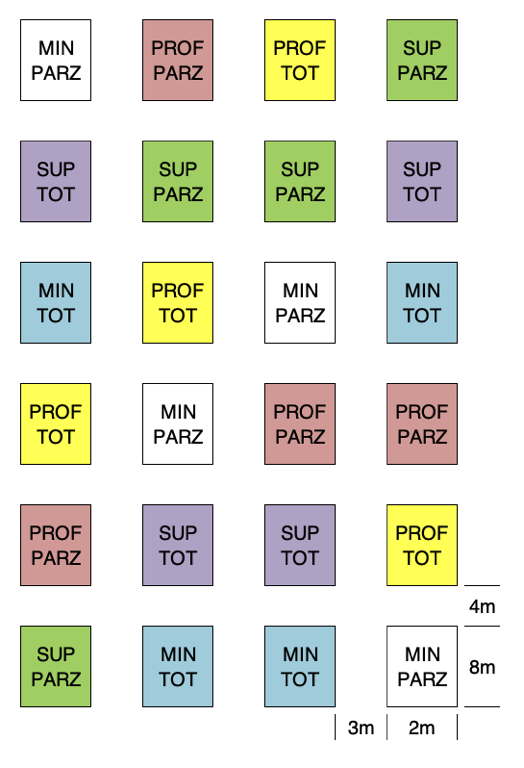
\includegraphics[width=0.65\linewidth]{_images/Mappa3FATT} 

}

\caption{Schema sperimentale fattoriale a blocchi randomizzati per l'Esempio 3}\label{fig:figName36}
\end{figure}

Questo disegno è totalmente appropriato, ma ci costringe a lasciare
parecchio spazio tra una parcella e l'altra, per poter manovrare con la
macchina per la lavorazione del terreno. Sarebbe utile raggruppare le
parcelle caratterizzate dalla stessa lavorazione, in modo da poter
lavorare su superfici più ampie. Ne guadagnerebbe l'uniformità
dell'esperimento e l'accuratezza dei risultati. Possiamo quindi
immaginare un disegno a un fattore, con parcelle di dimensione doppia
(\textbf{main-plots}), sulle quali eseguire, in modo randomizzato le
lavorazioni del terreno. Succesivamente, ogni main-plot può essere
suddivisa in due e, su ognuna delle due metà, possono essere allocati in
modo random i due trattamenti di diserbo. In questo modo ci troviamo ad
operare con parcelle di due dimensioni diverse: le main-plots per le
lavorazioni e le sub-plots per il diserbo. Questo tipo di schema prende
il nome di \textbf{parcella suddivisa} (\textbf{split-plot}), ed è
piuttosto comune nella sperimentazione di pieno campo.

Proviamo ad utilizzare R per redigere il piano sperimentale.

\begin{Shaded}
\begin{Highlighting}[]
\NormalTok{lavorazione <-}\StringTok{ }\KeywordTok{c}\NormalTok{(}\StringTok{"PROF"}\NormalTok{, }\StringTok{"SUP"}\NormalTok{, }\StringTok{"MIN"}\NormalTok{)}
\NormalTok{diserbo <-}\StringTok{ }\KeywordTok{c}\NormalTok{(}\StringTok{"TOT"}\NormalTok{, }\StringTok{"PARZ"}\NormalTok{)}
\NormalTok{designSPLIT <-}\StringTok{ }\KeywordTok{design.split}\NormalTok{(lavorazione, diserbo, }
  \DataTypeTok{r=}\DecValTok{4}\NormalTok{, }\DataTypeTok{serie=}\DecValTok{2}\NormalTok{, }\DataTypeTok{seed=}\DecValTok{777}\NormalTok{)}
\NormalTok{book <-}\StringTok{ }\NormalTok{designSPLIT}\OperatorTok{$}\NormalTok{book}
\NormalTok{book}
\NormalTok{##    plots splots block lavorazione diserbo}
\NormalTok{## 1    101      1     1         SUP    PARZ}
\NormalTok{## 2    101      2     1         SUP     TOT}
\NormalTok{## 3    102      1     1        PROF     TOT}
\NormalTok{## 4    102      2     1        PROF    PARZ}
\NormalTok{## 5    103      1     1         MIN    PARZ}
\NormalTok{## 6    103      2     1         MIN     TOT}
\NormalTok{## 7    104      1     2         SUP    PARZ}
\NormalTok{## 8    104      2     2         SUP     TOT}
\NormalTok{## 9    105      1     2         MIN     TOT}
\NormalTok{## 10   105      2     2         MIN    PARZ}
\NormalTok{## 11   106      1     2        PROF     TOT}
\NormalTok{## 12   106      2     2        PROF    PARZ}
\NormalTok{## 13   107      1     3         MIN     TOT}
\NormalTok{## 14   107      2     3         MIN    PARZ}
\NormalTok{## 15   108      1     3         SUP     TOT}
\NormalTok{## 16   108      2     3         SUP    PARZ}
\NormalTok{## 17   109      1     3        PROF     TOT}
\NormalTok{## 18   109      2     3        PROF    PARZ}
\NormalTok{## 19   110      1     4        PROF    PARZ}
\NormalTok{## 20   110      2     4        PROF     TOT}
\NormalTok{## 21   111      1     4         MIN     TOT}
\NormalTok{## 22   111      2     4         MIN    PARZ}
\NormalTok{## 23   112      1     4         SUP    PARZ}
\NormalTok{## 24   112      2     4         SUP     TOT}
\end{Highlighting}
\end{Shaded}

\begin{figure}

{\centering \includegraphics[width=0.65\linewidth]{_images/Mappa3SPLIT} 

}

\caption{Schema sperimentale split-plot a blocchi randomizzati per l'Esempio 3}\label{fig:figName37}
\end{figure}

In alcune circostanze, soprattutto nelle prove di diserbo chimico,
potrebbe trovare applicazione un altro tipo di schema sperimentale, nel
quale, in ogni blocco, un trattamento viene applicato a tutte le
parcelle di una riga e l'altro trattamento a tutte le parcelle di una
colonna. Ad esempio, il disegno sottostante mostra una prova nella quale
il terreno è stato diserbato in una striscia nel senso della lunghezza
e, dopo il diserbo, le colture sono state seminate in striscia, nel
senso della larghezza. Questo disegno è detto \textbf{strip-plot} ed è
molto comodo perché consente di lavorare velocemente.

\begin{figure}

{\centering 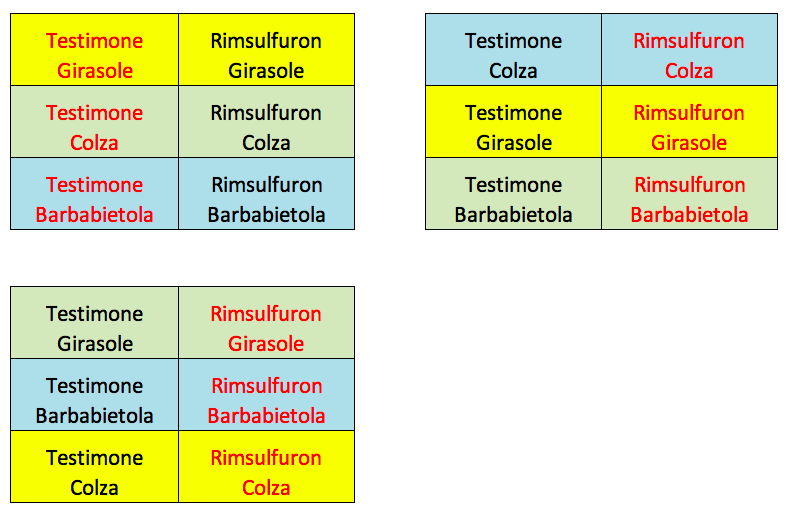
\includegraphics[width=0.9\linewidth]{_images/MappaStrip} 

}

\caption{Schema sperimentale a strip-plot}\label{fig:figName38}
\end{figure}

\subsection{Esempio 4}\label{esempio-4-1}

La prova di erba medica è fondamentalmente un esperimento a blocchi
randomizzati, il cui piano è riportato più sotto. Tuttavia, si tratta di
una coltura poiliennale nella quale ripeteremo le misurazioni ogni anno
sulle stesse parcelle. le misure ripetute non sono randomizzate (non
possono esserlo), ma seguono una metrica temporale. Proprio per questo
sviluppo lungo la scala del tempo, i dati che si raccolgono in questi
esperimenti a misure ripetute sono detti \textbf{dati longitudinali}.
Guardando bene il disegno si capisce anche per si parla di
\textbf{split-plot nel tempo}. Esempi affini sono relativi all'analisi
di accrescimento con misure non distruttive (esempio l'altezza) oppure i
prelievi di terreno a profondità diverse, anche se, in quest'ultimo
caso, la metrica delle misure ripetute è spaziale, non temporale.

Si può notare una certa analogia con il sottocampionamento illustrato
più sopra, nel senso che vengono prese più misure per parcella.
Tuttavia, bisogna tener presente che nel sottocampionamento le diverse
misure sono solo repliche e non vi è nessuna esigenza di distinguere tra
quelle prese nella stessa parcella. Invece, nel caso delle misure
ripetute ognuna di esse ha interesse individuale, in quanto espressione
di un'anno particolare.

\begin{figure}

{\centering 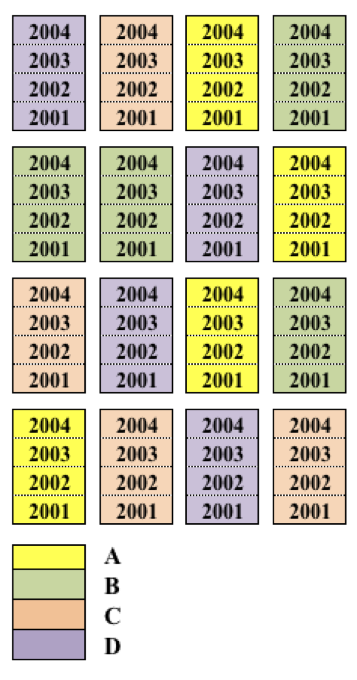
\includegraphics[width=0.55\linewidth]{_images/Mappa4} 

}

\caption{Schema sperimentale a blocchi randomizzati con misure ripetute (split-plot in time)}\label{fig:figName39}
\end{figure}

\subsection{Esempio 5}\label{esempio-5-1}

Per questo disegno osservazionale, la mappa non è necessaria. Tuttavia,
si può notare che, in ogni supermercato, abbiamo un disegno a
randomizzazione completa, con tre tipi di confezioni e tre repliche,
cioè nove confezioni scelte a random da un lotto più grande. Insomma, si
tratta di un esperimento ripetuto 9 volte che, pertanto, ha una certa
affinità con l'esperimento ripetuto dell'Esempio 2.

\section{Impianto delle prove}\label{impianto-delle-prove}

Da questo punto in poi, subentrano le competenze agronomiche e
fitopatologiche necessarie per codurre gli esperimenti, Mi piace solo
ricordare alcune pratiche usuali nella sperimentazione di pieno campo,
destinate a migliorare l'efficienza della prova.

\begin{enumerate}
\def\labelenumi{\arabic{enumi}.}
\tightlist
\item
  Seminare a densità più alte e poi diradare, per assicurare una
  migliore uniformità di impianto
\item
  Prelevare da ogni parcella più campioni ed, eventualmente,
  omogeneizzarli o mediare i risultati ottenuti (vedi il caso dei 1000
  semi)
\item
  Considerare le caratteristiche naturalmente meno variabili (es. la
  produzione areica e non la produzione per pianta)
\end{enumerate}

Voglio inoltre ricordare che gli esperimenti parcellari configurano una
situazione nella quale, per l'elevata cura che si pone nelle tecniche
agronomiche, si riesce ad ottenere una produttività almeno del 20\%
superiore rispetto a quanto avviene nella normale pratica agricola.

\section{Scrivere un progetto/report di ricerca: semplici
indicazioni}\label{scrivere-un-progettoreport-di-ricerca-semplici-indicazioni}

Quanto abbiamo finora esposto costituisce uno schema generale che può
essere adottato per redigere un progetto di ricerca o un report sui
risultati ottenuti (tesi, pubblicazione). Bisogna provare che la ricerca
che si è eseguita è precisa, accurata e replicabile/riproducibile e, di
conseguenza, i risultati sono validi.

Nella redazione di un progetto di ricerca o di un report, è fondamentale
tratteggiare bene i seguenti elementi:

\begin{enumerate}
\def\labelenumi{\arabic{enumi}.}
\tightlist
\item
  Titolo della ricerca
\item
  Descrizione del problema e background scientifico
\item
  Ipotesi scientifica, motivazioni e obiettivi
\item
  Tipo di esperimento e durata
\item
  Disegno sperimentale: trattamenti sperimentali (tesi) a confronto con
  dettagli relativi all'applicazione
\item
  Unità sperimentali e criteri per la loro selezione. Dettagli su
  repliche e randomizzazione
\item
  Dettagli su eventuali tecniche di `blocking'
\item
  Variabili da rilevare/rilevate
\item
  Dettagli su come le variabili saranno/sono state rilevate
\item
  Esposizione dei risultati (solo report)
\item
  Discussione (solo report)
\item
  Conclusioni (solo report)
\end{enumerate}

Alcuni aspetti che divengono elemento di valutazione del progetto e/o
del report sono i seguenti:

\begin{enumerate}
\def\labelenumi{\arabic{enumi}.}
\tightlist
\item
  La selezione dei metodi deve essere coerente con gli obiettivi
\item
  Descrizione dettagliata dei materiali e metodi (bisogna che chiunque
  sia in grado di replicare l'esperimento)
\item
  Esposizione dei risultati chiara e convincente
\item
  Discussione approfondita e con molti riferimenti alla letteratura.
\end{enumerate}

\chapter{\texorpdfstring{Modelli matematici a `due
facce'}{Modelli matematici a due facce}}\label{modelli-matematici-a-due-facce}

L'eredità galileiana ci porta ad immaginare che il funzionamento della
natura sia basato su una serie di relazioni causa-effetto, descrivibili
utilizzando il linguaggio universale della matematica. La conoscenza
esatta di queste relazioni, nella teoria, ci potrebbe consentire di
prevedere l'andamento di ogni fenomeno naturale, almeno quelli
osservabili con sufficiente precisione.

In effetti era proprio questa l'ambizione più grande degli scienziati
all'inizio dell'ottocento: conoscendo lo stato iniziale di un sistema,
doveva essere possibile prevederne l'evoluzione futura. In realtà si è
ben presto scoperto che si trattava di un'ambizione irrealistica, non
tanto e non solo per la comparsa della meccanica quantistica un secolo
dopo, ma anche per l'aumento di importanza degli studi in ambito
psichiatrico e medico/biologico. Questi studi, infatti, venivano (e
vengono) eseguiti su organismi viventi altamente complessi, che, se
sottoposti allo stesso stimolo, danno risposte altamente variabili e,
spesso, anche difficilmente misurabili e controllabili. Immaginiamo
quanto possa essere difficile quantificare uno stato legato ad una
patologia mentale e individuare un pattern di risposta ad un certo
stimolo, ad esempio farmacologico.

Queste difficoltà fecero prevalere, tra i biologi, la convinzione che la
natura funzionasse in base a meccanismi deterministici ben definiti,
anche se difficilmente osservabili nella pratica sperimentale, a causa
dei numerosi elementi di incertezza che si manifestavano nel corso delle
osservazioni sperimentali. Insomma, la natura è perfetta, ma
l'osservazione è fallace, perché influenzata dalla presenza di una forte
componente stocastica e imprevedibile, che va sotto il nome generico di
'errore sperimentale'.

Dell'errore sperimentale abbiamo già parlato nei capitoli precedenti.
Abbiamo anche visto che Ronald Fisher, nel suo famoso testo ``Il disegno
degli esperimenti'' ha posto le basi per una corretta metodica
sperimentale, volta a minimizzare l'impatto della componente stocastica
e, soprattutto, ad impedire che essa possa confondersi con gli effetti
degli stimoli sperimentali in studio. Minimizzare, tuttavia, non
significa eliminare ed è evidente che, pur con tutti gli sforzi
possibili, i risultati sperimentali saranno influenzati sempre e
comunque da una certa quota di variabilità stocastica. Si vengono quindi
a creare due contrapposte situazioni:

\begin{enumerate}
\def\labelenumi{\arabic{enumi}.}
\tightlist
\item
  la verità `vera', immanente, di natura fondamentalmente deterministica
  e legata a relazioni causa-effetto ben definite.
\item
  La `verità' sperimentale, che si produce a partire dalla verità
  `vera', per effetto dell'azione di elementi perturbativi casuali, che
  non ci permettono di osservare la verità `vera'.
\end{enumerate}

Tenendo conto di questo, nella logica galileiana, possiamo provare ad
utilizzare dei modelli matematici per descrivere le nostre osservazioni
sperimentali e come esse si producono.

\section{\texorpdfstring{Verità `vera' e modelli
deterministici}{Verità vera e modelli deterministici}}\label{verita-vera-e-modelli-deterministici}

In semplice linguaggio algebrico, potremmo immaginare che la natura
opera secondo un modello deterministico causa-effetto di questo tipo:

\[ Y_E = f(X, \theta) \]

dove \(Y_E\) è l'effetto atteso dello stimolo \(X\), secondo la funzione
\(f\), basata su una collezioni di parametri \(\theta\).

In questo modello vi sono una serie di componenti, che proviamo a
guardare un po' più nel dettaglio.

La risposta attesa (\(Y_E\)) è l'oggetto del nostro studio e può
assumere le forme più disparate: spesso è numerica, ma a volte
rappresenta una qualità. In questo libro consideremo solo la situazione
in cui \(Y\) è rappresentato da una sola variabile (analisi univariate),
ma esistono casi in cui viene osservata e analizzata la risposta di
soggetti in relazione a molte variabili risposta (analisi multivariate).

Lo stimolo sperimentale (\(X\)) è costituito da una o più variabili
continue, discrete o categoriche, che rappresenta/ano il/i trattamento/i
sperimentale/i (fattore/i sperimentale/i). Insieme ad \(Y\) è l'elemento
noto di un esperimento, in quanto viene definito \emph{a priori} con il
disegno sperimentale.

La `funzione' di risposta (\(f\)) è un'equazione, altrimenti detta
`modello matematico'. L'equazione può essere lineare o non-lineare ed è
selezionata o in base a considerazioni di carattere biologico, o con un
approccio puramente empirico, nel quale osservo la risposta e scelgo
un'equazione la cui forma si adatta bene ad essa.

I parametri di una funzione (\(\theta\)) sono un insieme di valori
numerici che definiscono il modello. Nel prossimo paragrafo vedremo
qualche esempio.

\section{Qualche esempio di modello
deterministico}\label{qualche-esempio-di-modello-deterministico}

Il modello più semplice è il cosiddetto modello della media:

\[ Y = \mu \]

Con questo modello si vuole indicare che un'osservazione dovrebbe
conformarsi ad un certo valore atteso, in assenza di ogni stimolo
sperimentale noto. Ha un solo parametro, cioè \(\mu\).

Un modello appena più complesso è il cosidetto modello ANOVA:

\[
Y = \left\{ {\begin{array}{ll}
\mu_1 & se \quad X = A \\
\mu_2 & se \quad X = B
\end{array}} \right.
\]

In questo caso la risposta attesa dipende dallo stimolo sperimentale X,
che è composto di due trattamenti: se il soggetto è trattato con A,
fornisce la risposta \(\mu_1\), se è trattato con B fornisce \(\mu_2\).
Il trattamento sperimentale è costituito da una variabile categorica con
due modalità, ma l'estensione a più modalità è immediata. In questo
caso, abbiamo due parametri (\(\mu_1\) e \(\mu_2\)).

Un ulteriore esempio di modello che vedremo in questo libro è la
regressione lineare semplice, dove la relazione di risposta è
descrivibile con una retta, la cui equazione generale è:

\[ Y = a + b \times X \]

In questo caso sia la \(Y\) che la \(X\) sono variabili quantitative e
vi sono due parametri \(a\) e \(b\).

I modelli finora descritti sono lineari, ma esistono numerosi funzioni
che descrivono relazioni curvilinee. Come esempio possiamo citare la
parabola:

\[ Y = a + b \times X + c \times X^2\] caratterizzata da tre parametri,
oppure la funzione esponenziale:

\[ Y = a \, e^{b X} \]

caratterizzata da due parametri (\(a\) e \(b\)), mentre \(e\) è
l'operatore di Nepero. Delle funzioni curvilinea parleremo al termine di
questo libro.

\section{Genesi deterministica delle osservazioni
sperimentali}\label{genesi-deterministica-delle-osservazioni-sperimentali}

Le espressioni date più sopra sono tutte nella loro forma generale e non
sono utilizzabili se ai parametri non viene sostituito un valore
numerico. E'proprio questo il nostro punto di partenza: un fenomeno
scientifico può essere determinato (meglio, descritto) attraverso
un'equazione e dei parametri.

Ad esempio, potremmo immaginare che la risposta produttiva (Y) di una
coltura (es. frumento) dipenda dalla dose della concimazione azotata
(X), seguendo un andamento lineare, con \(a = 20\) e \(b = 0.3\).
Rifacendosi alla notazione esposta sopra diremmo che \(\theta\) è
l'insieme dei valori 20 e 0.3.

Se questo assunto è vero, un eventuale esperimento di concimazione
azotata, in assenza di qualunque fattore perturbativo, dovrebbe dare
risultati assolutamento prevedili. Ad esempio, se concimiamo il frumento
con 0, 30, 60, 90, 120 e 150 kg/ha di azoto, dovremmo osservare le
risposte riportate qui di seguito.

\begin{Shaded}
\begin{Highlighting}[]
\NormalTok{X <-}\StringTok{ }\KeywordTok{c}\NormalTok{(}\DecValTok{0}\NormalTok{, }\DecValTok{30}\NormalTok{, }\DecValTok{60}\NormalTok{, }\DecValTok{90}\NormalTok{, }\DecValTok{120}\NormalTok{, }\DecValTok{150}\NormalTok{)}
\NormalTok{Ye <-}\StringTok{ }\DecValTok{20} \OperatorTok{+}\StringTok{ }\FloatTok{0.3} \OperatorTok{*}\StringTok{ }\NormalTok{X}
\NormalTok{Ye}
\NormalTok{## [1] 20 29 38 47 56 65}
\end{Highlighting}
\end{Shaded}

Qualcuno potrebbe obiettare che si tratta di una situazione
irrealistica, perché la relazione tra concimazione azotata e produzione
del frumento non è lineare. Non importa, in questo momento vogliamo
semplicemente illustrare qual è la genesi delle osservazioni
sperimentali. Fondamentalmente postuliamo l'esistenza di un modello
matematico deterministico (causa-effetto) che, in assenza di errore
sperimentale, è in grado di descrivere il comportamento della natura in
una data situazione pedo-climatica.

\section{Errore sperimentale e modelli
stocastici}\label{errore-sperimentale-e-modelli-stocastici}

Tuttavia esiste un problema: l'errore sperimentale, puramente
stocastico, confonde le nostre osservazioni e le rende diverse da quanto
previsto dal modello deterministico. Come fare per incorporare questi
effetti stocastici in un modello matematico? Ne parliamo immediatamente
attraverso un esempio, semplice, ma concreto.

Immaginiamo un campo di frumento, di notevoli dimensioni. Un campo nella
valle del Tevere, con milioni di piante geneticamente simili, in un
ambiente abbastanza uniforme da un punto di vista del microclima.
Immaginiamo di voler determinare l'altezza delle piante di questo campo.
Immaginiamo di non avere limitazioni e di poter determinare l'altezza di
tutte le piante dell'appezzamento. La nostra popolazione di soggetti
diviene una popolazione di misure. Come è fatta questa popolazione?
Quali sono le sue caratteristiche? Basiamoci sulla nostra esperienza
professionale, cercando di utilizzare argomenti che possano essere
condivisibili per l'intera comunità scientifica.

In primo luogo, possiamo dire che l'altezza delle piante dovrebbe essere
quella dettata dal loro patrimonio genetico. Poniamo che questa altezza
sia \(\mu = 100\); di conseguenza, il valore atteso di altezza è:

\[Y_E  = \mu = 100\]

In realtà, questo valore \(\mu\) non è osservabile, a causa dell'errore
sperimentale. Al suo posto osserveremo \(Y_O \neq Y_E\), con:

\[ Y_O = \mu + \varepsilon \]

dove \(\varepsilon\) è appunto una misura della componente stocastica
individuale che distorce i risultati. Che valori potrebbe assumere
\(\varepsilon\)? I valori individuali non possiamo conoscerli, ma
possiamo fare alcune considerazioni probabilistiche: se il valore atteso
è 100, trovare altezze comprese tra 99 e 101 cm dovrebbe essere molto
più frequente che non trovare altezze pari a 40 cm o 180 cm. Quindi
trovare valori di \(\varepsilon\) vicini allo 0 dovrebbe essere molto
più frequente che non trovarli lontani.

In generale, esiste una funzione che ci permetta di assegnare valori di
probabilità alle diverse altezze che possiamo trovare in un campo di
frumento? La risposta è si: funzioni di questo tipo si chiamano
\textbf{funzioni di probabilità}.

\subsection{Funzioni di probabilità}\label{funzioni-di-probabilita}

Se avessimo rilevato una qualità del soggetto, come il sesso (M/F), la
mortalità (vivo/morto), la germinabilità (germinato/non germinato),
avremmo una variabile categorica nominale e potremmo calcolare le
probabilità definita come rapporto tra il numero degli eventi favorevoli
e il numero totale di eventi possibili (probabilità `frequentista').

Ad esempio, immaginiamo di aver rilevato il numero di germogli di
accestimento di 20 piante di frumento e di averne trovate 4 con 0
germigli, 6 con 1 germoglio, 8 con due germogli e 2 con tre germogli. La
funzione che assegna la probabilità P ad ognuno dei quattro eventi X
possibili (\textbf{funzione di probabilità}) è:

\[
P(X) = \left\{ \begin{array}{l}
 4/20 = 0.2 \,\,\,\,\,\,se\,\,\,\,\,\,X = 0 \\ 
 6/20 = 0.3 \,\,\,\,\,\,se\,\,\,\,\,\,X = 1 \\ 
 8/20 = 0.4\,\,\,\,\,\,se\,\,\,\,\,\, X = 2 \\ 
 2/20 = 0.1 \,\,\,\,\,\,se\,\,\,\,\,\,X = 3 \\ 
 \end{array} \right.
\]

Viene ad essere definita una \textbf{distribuzione di probabilità}, che
ha due caratteristiche importanti:

\begin{enumerate}
\def\labelenumi{\arabic{enumi}.}
\tightlist
\item
  P(X) è sempre non-negativo (ovvio! le probabilità sono solo positive o
  uguali a 0);
\item
  la somma delle probabilità di tutti gli eventi è sempre pari ad 1
  (ovvio anche questo: la probabilità che capiti uno qualunque degli
  eventi è sempre 1).
\end{enumerate}

Se gli eventi possibili sono ordinabili (come nel caso precedente),
oltre alla funzione di probabilità, si può definire anche la
\textbf{funzione di probabilità cumulata}, detta anche \textbf{funzione
di ripartizione} con la quale si assegna ad ogni evento la sua
probabilità più quella di tutti gli eventi `inferiori'. Nell'esempio
precedente:

\[
P(X) = \left\{ \begin{array}{l}
 0.2\,\,\,\,\,\,se\,\,\,\,\,\,X \leq 0 \\ 
 0.5\,\,\,\,\,\,se\,\,\,\,\,\,X \leq 1 \\ 
 0.9\,\,\,\,\,\,se\,\,\,\,\,\,X \leq 2 \\ 
 1.0\,\,\,\,\,\,se\,\,\,\,\,\,X \leq 3 \\ 
 \end{array} \right.
\]

Per una distribuzione di probabilità come questa (classi numeriche
ordinate), considerando il valore centrale di ogni classe, possiamo
calcolare la media (valore atteso) come:

\[
\mu  = E(X) = \sum{\left[ x_i \cdot P(X = x_i ) \right]}
\]

e la varianza come:

\[\sigma ^2  = Var(X) = E\left[ {X - E(X)} \right]^2  = \sum{ \left[ {\left( {x_i  - \mu } \right)^2 \cdot P(X = x_i )} \right]}\]

In questo caso specifico, la media è pari a:

\begin{Shaded}
\begin{Highlighting}[]
\NormalTok{mu <-}\StringTok{ }\DecValTok{0} \OperatorTok{*}\StringTok{ }\FloatTok{0.2} \OperatorTok{+}\StringTok{ }\DecValTok{1} \OperatorTok{*}\StringTok{ }\FloatTok{0.3} \OperatorTok{+}\StringTok{ }\DecValTok{2} \OperatorTok{*}\StringTok{ }\FloatTok{0.4} \OperatorTok{+}\StringTok{ }\DecValTok{3} \OperatorTok{*}\StringTok{ }\FloatTok{0.1}
\NormalTok{mu}
\NormalTok{## [1] 1.4}
\end{Highlighting}
\end{Shaded}

e la varianza è pari a:

\begin{Shaded}
\begin{Highlighting}[]
\NormalTok{(}\DecValTok{0} \OperatorTok{-}\StringTok{ }\NormalTok{mu)}\OperatorTok{^}\DecValTok{2} \OperatorTok{*}\StringTok{ }\FloatTok{0.2} \OperatorTok{+}\StringTok{ }\NormalTok{(}\DecValTok{1} \OperatorTok{-}\StringTok{ }\NormalTok{mu)}\OperatorTok{^}\DecValTok{2} \OperatorTok{*}\StringTok{ }\FloatTok{0.3} \OperatorTok{+}\StringTok{ }\NormalTok{(}\DecValTok{2} \OperatorTok{-}\StringTok{ }\NormalTok{mu)}\OperatorTok{^}\DecValTok{2} \OperatorTok{*}\StringTok{ }\FloatTok{0.3} \OperatorTok{+}
\StringTok{  }\NormalTok{(}\DecValTok{3} \OperatorTok{-}\StringTok{ }\NormalTok{mu)}\OperatorTok{^}\DecValTok{2} \OperatorTok{*}\StringTok{ }\FloatTok{0.2}
\NormalTok{## [1] 1.06}
\end{Highlighting}
\end{Shaded}

Mediamente, le nostre piante hanno 1.4 germogli con una varianza pari a
1.06.

\subsection{Funzioni di densità}\label{funzioni-di-densita}

Quanto abbiamo detto finora non si applica al nostro caso, in quanto
abbiamo rilevato una variabile continua (altezza) e non abbiamo
intenzione di discretizzarla in classi. In questo caso le altezze che
possiamo riscontrare sono pressoché infinite e non ha molto senso
chiedersi, ad esempio, qual è la probabilità di trovare un individuo
alto esattamente 96 cm. Capiamo da soli che questa probabilità è un
infinitesimo.

Al contrario, come abbiamo visto più sopra, possiamo calcolare la
probabilità di ottenere un valore compreso in un intervallo, per esempio
da 80 a 90 cm. Tuttavia, abbiamo detto di non voler discretizzare, anche
perché la probabilità dipenderebbe dall'ampiezza dell'intervallo
prescelto, il che introdurrebbe un elemento arbitrario. Possiamo
tuttavia pensare di calcolare la \textbf{densità di probabilità}, vale a
dire il rapporto tra la probabilità di un intervallo e la sua ampiezza
(cioè la probabilità per unità di ampiezza dell'intervallo; per questo
si parla di densità). E' evidente che se un intervallo diventa
infinitamente piccolo anche la probabilità tende a zero con la stessa
`velocità', in modo che la densità di probabilità tende ad un numero
finito (ricordate il limite del rapporto di polinomi?).

Insomma, con i fenomeni continui non possiamo lavorare con la
probabilità dei singoli eventi, ma possiamo lavorare con la densità di
probabilità e definire quindi apposite \textbf{funzioni di densità}.
Analogamente alle funzioni di probabilità, le funzioni di densità
debbono avere due caratteristiche:

\begin{enumerate}
\def\labelenumi{\arabic{enumi}.}
\tightlist
\item
  assumere solo valori non-negativi;
\item
  la somma delle probabilità di tutti gli eventi possibili, calcolabile
  come integrale della funzione di densità, deve essere unitaria (anche
  in questo caso la densità di probabilità di tutti gli eventi possibili
  è pari ad 1).
\end{enumerate}

Data una funzione di densità, possiamo costruire la corrispondente
\textbf{funzione di probabilità cumulata}, facendo l'integrale per ogni
evento pari o inferiore a quello dato. Più in generale, per variabili
continue sia la funzione di ripartizione (probabilità cumulata), che la
media o la devianza sono definite ricorrendo agli integrali:

\[ \begin{array}{l}
P(X) = f(x) \\ 
P(X \le x) = \int\limits_{ - \infty }^x {f(x)} dx \\ 
\mu  = E(X) = \int\limits_{ - \infty }^{ + \infty } {xf(x)} dx \\ 
\sigma ^2  = Var(X) = \int\limits_{ - \infty }^{ + \infty } {\left( {x - \mu } \right)^2 f(x)} dx \\ 
\end{array} \]

In pratica, vedremo che, a seconda della funzione di densità, è
possibile adottare formule semplificate per le diverse statistiche
descrittive.

\section{La distribuzione normale (curva di
Gauss)}\label{la-distribuzione-normale-curva-di-gauss}

Torniamo ancora alla nostra popolazione di misure, relative alle altezze
del frumento nella media Valle del Tevere. E' ragionevole pensare che,
effettuando le misurazioni con uno strumento sufficientemente preciso e
in presenza delle sole variazioni casuali (visto che abbiamo idealmente
rimosso ogni differenza sistematica spiegabile), i risultati tendono a
differire tra di loro, muovendosi intorno ad un valore medio, rispetto
al quale le misure superiori ed inferiori sono equiprobabili e tendono
ad essere più rare, via via che ci si allontana dal valore medio. Questo
ragionamento ci porta verso una densità di probabilità (parliamo di
variabili continue) a forma di campana, che potrebbe essere descritta
con una funzione continua detta \textbf{curva di Gauss}.

La curva è descritta dalla seguente funzione di densità:

\[P(x) = \frac{1}{{\sigma \sqrt {2\pi } }}\exp \left[{\frac{\left( {x - \mu } \right)^2 }{2\sigma ^2 }} \right]\]

ove \(P(x)\) è la densità di probabilità di una certa misura \(x\),
mentre \(\mu\) e \(\sigma\) sono rispettivamente la media e la
deviazione standard della popolazione (per la dimostrazione si rimanda a
testi specializzati). Le variabili casuali che possono essere descritte
con la curva di Gauss, prendono il nome di \emph{variabili normali} o
\emph{normalmente distribuite}.

Studiare le principali proprietà matematiche della curva di Gauss è
estremamente utile. Ad esempio, senza voler entrare troppo nel
dettaglio, guardando la curva di Gauss possiamo notare che:

\begin{enumerate}
\def\labelenumi{\arabic{enumi}.}
\tightlist
\item
  la forma della curva dipende da solo da \(\mu\) e \(\sigma\) (figura
  @ref\{fig:figName51\}). Ciò significa che, se prendiamo un gruppo di
  individui e partiamo dal presupposto (\textbf{assunzione parametrica})
  che in relazione ad un determinato carattere quantitativo (es.
  produzione) la distribuzione di frequenza è normale (e quindi può
  essere descritta con una curva di Gauss), allora basta conoscere la
  media e la deviazione standard degli individui e immediatamente
  conosciamo l'intera distribuzione di frequenza (cioè l'intera
  popolazione di misure);
\item
  la curva ha due asintoti e tende a 0 quando x tende a infinito. Questo
  ci dice che se assumiamo che un fenomeno è descrivibile con una curva
  di Gauss, allora assumiamo che tutte le misure sono possibili, anche
  se la loro frequenza decresce man mano che ci si allontana dalla
  media;
\item
  la probabilità che la x assuma valori compresi in un certo intervallo
  è data dall'integrale della curva di Gauss in quell'intervallo. Ad
  esempio, la figura @ref\{fig:figName52\} mostra l'80° percentile, cioè
  la misura più alta dell'80\% delle misure possibili;
\item
  Se la curva di Gauss è stata costruita utilizzando le frequenze
  relative, l'integrale della funzione è uguale ad 1. Infatti la somma
  delle frequenze relative di tutte le varianti possibili non può che
  essere uguale ad 1;
\item
  la curva è simmetrica. Questo indica che la frequenza dei valori
  superiori alla media è esattamente uguale alla frequenza dei valori
  inferiori alla media.
\item
  dato \(\sigma\), possiamo dire che la frequenza dei valori superiori a
  \(\mu + \sigma\) è pari al 15.87\% ed è uguale alla frequenza dei
  valori inferiori a \(\mu - \sigma\).
\end{enumerate}

\begin{figure}

{\centering 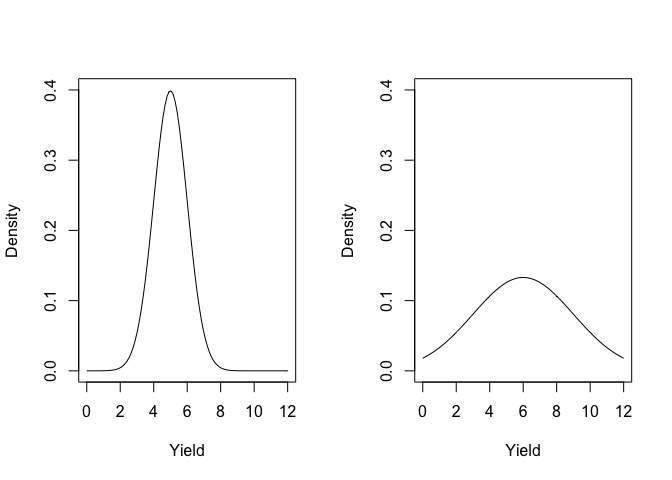
\includegraphics[width=0.9\linewidth]{_main_files/figure-latex/figName51-1} 

}

\caption{Distribuzioni normali con diversa media e deviazione standard (rispettivamente 5 e 1 a sinistra, 6 e 3 a destra}\label{fig:figName51}
\end{figure}

\begin{figure}

{\centering 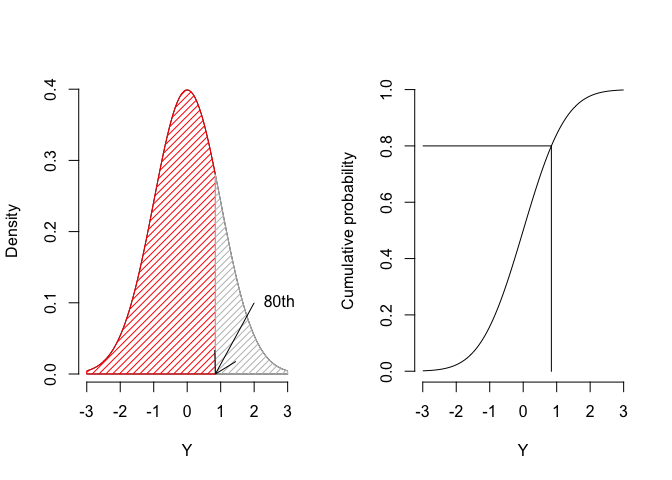
\includegraphics[width=0.9\linewidth]{_main_files/figure-latex/figName52-1} 

}

\caption{Integrale della curva di densità normale (80° percentile; sinistra) e curva di probabilità cumulata (destra)}\label{fig:figName52}
\end{figure}

\section{\texorpdfstring{Modelli `a due
facce'}{Modelli a due facce}}\label{modelli-a-due-facce}

A questo punto, sempre in relazione all'altezza del nostro frumento,
possiamo scrivere che l'altezza della pianta \(i\) è:

\[Y_i = \mu + \varepsilon\] dove:

\[ \varepsilon \sim N(0, \sigma) \]

cioè la componente stocastica \(\varepsilon\) è normalmente distribuita
con media 0 e deviazione standard \(\sigma\). E'abbastanza evidente che
è possibile scrivere:

\[Y_i \sim N(\mu, \varepsilon)\]

cioè che l'altezza del frumento è normalmente distribuita con media
\(\mu\) e deviazione standard \(\sigma\). Dato che si tratta di una
semplice traslazione di una distribuzione normale lungo l'asse delle
ascisse (come in figura \#ref\{figName51\}), le due espressioni sono
totalmente equivalenti.

Ora si può dire che conosciamo perfettamente la popolazione di partenza
se conosciamo \(\mu\) e \(\sigma\), cioè la parte (`faccia')
deterministica e la parte (`faccia') stocastica del modello. Se quindi
immaginiamo che \(\mu = 100\) (come abbiamo detto in precedenza) e
\(\sigma = 8\), possiamo risolvere alcuni semplici esercizi, utilizzando
le funzioni di calcolo di probabilità di R.

\subsection{Esercizio 1}\label{esercizio-1}

Calcolare la densità di un'altezza pari a 120 cm.

\begin{Shaded}
\begin{Highlighting}[]
\KeywordTok{dnorm}\NormalTok{(}\DecValTok{120}\NormalTok{, }\DataTypeTok{mean =} \DecValTok{100}\NormalTok{, }\DataTypeTok{sd =} \DecValTok{8}\NormalTok{)}
\NormalTok{## [1] 0.002191038}
\end{Highlighting}
\end{Shaded}

\subsection{Esercizio 2}\label{esercizio-2}

Qual è la probabilità di ottenere piante con altezza inferiore a 80 cm?

\begin{Shaded}
\begin{Highlighting}[]
\KeywordTok{pnorm}\NormalTok{(}\DecValTok{80}\NormalTok{, }\DataTypeTok{mean =} \DecValTok{100}\NormalTok{, }\DataTypeTok{sd =} \DecValTok{8}\NormalTok{)}
\NormalTok{## [1] 0.006209665}
\end{Highlighting}
\end{Shaded}

\subsection{Esercizio 3}\label{esercizio-3}

Qual è la probabilità di ottenere piante con altezza superiore a 110 cm?

\begin{Shaded}
\begin{Highlighting}[]
\KeywordTok{pnorm}\NormalTok{(}\DecValTok{110}\NormalTok{, }\DataTypeTok{mean =} \DecValTok{100}\NormalTok{, }\DataTypeTok{sd =} \DecValTok{8}\NormalTok{, }\DataTypeTok{lower.tail =}\NormalTok{ F)}
\NormalTok{## [1] 0.1056498}
\end{Highlighting}
\end{Shaded}

Si utilizza l'argomento lower.tail=FALSE, in quanto stiamo cercando la
probabilità di un'a concentrazione pari o superiore ad 1.1, e non pari
od inferiore.`altezza pari o superiore a 110 cm (upper-tail) e non
quella pari o inferiore a 110 cm (lower-tail), che sarebbe fornita di
default. E' totalmente equivalente utilizzare la funzione sottostante.

\begin{Shaded}
\begin{Highlighting}[]
\DecValTok{1} \OperatorTok{-}\StringTok{ }\KeywordTok{pnorm}\NormalTok{(}\DecValTok{110}\NormalTok{, }\DataTypeTok{mean =} \DecValTok{100}\NormalTok{, }\DataTypeTok{sd =} \DecValTok{8}\NormalTok{)}
\NormalTok{## [1] 0.1056498}
\end{Highlighting}
\end{Shaded}

\subsection{Esercizio 4}\label{esercizio-4}

Qual è la probabilità di ottenere piante con altezza compresa tra 80 e
110 cm?

\begin{Shaded}
\begin{Highlighting}[]
\KeywordTok{pnorm}\NormalTok{(}\DecValTok{110}\NormalTok{, }\DataTypeTok{mean =} \DecValTok{100}\NormalTok{, }\DataTypeTok{sd =} \DecValTok{8}\NormalTok{) }\OperatorTok{-}\StringTok{ }\KeywordTok{pnorm}\NormalTok{(}\DecValTok{80}\NormalTok{, }\DataTypeTok{mean =} \DecValTok{100}\NormalTok{, }\DataTypeTok{sd =} \DecValTok{8}\NormalTok{)}
\NormalTok{## [1] 0.8881406}
\end{Highlighting}
\end{Shaded}

\subsection{Esercizio 5}\label{esercizio-5}

Qual è quella misura che è superiore al 90\% di tutte le piante del
campo (90° percentile?

\begin{Shaded}
\begin{Highlighting}[]
\KeywordTok{qnorm}\NormalTok{(}\FloatTok{0.9}\NormalTok{, }\DecValTok{100}\NormalTok{, }\DecValTok{8}\NormalTok{)}
\NormalTok{## [1] 110.2524}
\end{Highlighting}
\end{Shaded}

\subsection{Esercizio 6}\label{esercizio-6}

Qual è quella misura che è inferiore al 20\% di tutte le piante del
campo (80° percentile?

\begin{Shaded}
\begin{Highlighting}[]
\KeywordTok{qnorm}\NormalTok{(}\FloatTok{0.8}\NormalTok{, }\DecValTok{100}\NormalTok{, }\DecValTok{8}\NormalTok{)}
\NormalTok{## [1] 106.733}
\KeywordTok{qnorm}\NormalTok{(}\FloatTok{0.2}\NormalTok{, }\DecValTok{100}\NormalTok{, }\DecValTok{8}\NormalTok{, }\DataTypeTok{lower.tail=}\NormalTok{F)}
\NormalTok{## [1] 106.733}
\end{Highlighting}
\end{Shaded}

\subsection{Esercizio 7}\label{esercizio-7}

Quali sono quei due valori, simmetrici rispetto alla media e tali da
formare un intervallo all'interno del quale cadono il 95\% delle piante?

\begin{Shaded}
\begin{Highlighting}[]
\KeywordTok{qnorm}\NormalTok{(}\FloatTok{0.025}\NormalTok{, }\DecValTok{100}\NormalTok{, }\DecValTok{8}\NormalTok{)}
\NormalTok{## [1] 84.32029}
\KeywordTok{qnorm}\NormalTok{(}\FloatTok{0.975}\NormalTok{, }\DecValTok{100}\NormalTok{, }\DecValTok{8}\NormalTok{)}
\NormalTok{## [1] 115.6797}
\end{Highlighting}
\end{Shaded}

\section{Altri modelli stocastici di interesse per lo
sperimentatore}\label{altri-modelli-stocastici-di-interesse-per-lo-sperimentatore}

Oltre alla distribuzione gaussiana, che è largamente la più importante,
esistono molti altri modelli stocastici, sia per eventi continui che
discreti. Menzioniamo solamente la distribuzione \(t\) di Student, la
distribuzione binomiale, la distribuzione \(\chi^2\) e la distribuzione
\(F\) di Fisher. Chi volesse approfondire queste distribuzioni trova
informazioni in seguito. Per gli altri vogliamo solo far notare che le
funzioni di R per il calcolo di probabilità hanno sempre la stessa
sintassi, che, dato il nome della distribuzione (es. `norm' per la
distribuzione normale), assegna il prefisso `d' per la funzione di
probabilità/densità, `p' per la funzione di probabilità cumulata, `q'
per la funzione quantile. Alcuni esempi sono dati nel quadro sottostante

\begin{verbatim}
# BINOMIALE
dbinom()
pbinom()
qbinom()

# t di Student
dt()
pt()
qt
\end{verbatim}

\section{E allora?}\label{e-allora}

Cerchiamo di ricapitolare. Le popolazioni di soggetti sperimentali e
delle loro misure sono un oggetto largamente ignoto e inconoscibile.
Infatti, le caratteristiche dei soggetti della popolazione sono, in
parte, determinate in base a relazioni causa-effetto, ma, in altra
parte, esse sono puramente stocastiche. Tuttavia è ragionevole supporre
che esse seguano una qualche funzione di probabilità/densità
(\textbf{assunzione parametrica}). Se questo è vero, allora possiamo
utilizzare queste funzioni e i loro integrali per calcolare la
probabilità di ottenere una certa misura o un certo insieme di misure.

\section{Le simulazioni Monte Carlo}\label{le-simulazioni-monte-carlo}

Se quanto abbiamo detto è vero, ogni esperimento scientifico non è altro
che un'operazione di campionamento da una certa distribuzione di
probabilità. Questo campionamento può essere simulato impiegando un
generatore di numeri casuali. Immaginiamo di avere disegnato un
esperimento con otto parcelle (repliche) per determinare la produzione
del mais in un certo appezzamento e immaginiamo che queste parcelle
costituiscano un campione rappresentativo della popolazione di parcelle
di quell'appezzamento. Se la popolazione è distribuita normalmente, con
media pari a 12 t/ha e deviazione standard pari ad 1.2 t/ha, allora
possiamo simulare i risultati del nostro esperimento come segue:

\begin{Shaded}
\begin{Highlighting}[]
\KeywordTok{set.seed}\NormalTok{(}\DecValTok{1234}\NormalTok{)}
\NormalTok{Y <-}\StringTok{ }\KeywordTok{rnorm}\NormalTok{(}\DecValTok{8}\NormalTok{, }\DecValTok{15}\NormalTok{, }\FloatTok{1.2}\NormalTok{)}
\NormalTok{Y}
\NormalTok{## [1] 15.51584 14.47349 13.56998 13.70647 14.85936 14.12243 14.80915 13.61789}
\KeywordTok{mean}\NormalTok{(Y)}
\NormalTok{## [1] 14.33433}
\KeywordTok{sd}\NormalTok{(Y)}
\NormalTok{## [1] 0.7023494}
\end{Highlighting}
\end{Shaded}

La generazione di numeri casuali con il computer viene fatta attraverso
algoritmi che, a partire da un \emph{seed} iniziale, forniscono sequenze
che obbediscono a certe proprietà fondamentali (numeri pseudo-casuali).
Il comando `set.seed(1234)' ci permette di partire dallo stesso valore e
quindi di ottenere lo stesso campione. Un'altra cosa da notare è che il
nome della funzione che genara numeri casuali è formato con il nome
della distribuzione (`norm') più il prefisso `r'. Questo è vero per
tutte le altre distribuzioni in R (`rbinom', `rt' e così via)

I valori campionati non riflettono le caratteristiche della popolazione,
nel senso che la media e la deviazione standard del campione
differiscono da quelle della popolazione. E' esattamente ciò che capita
durante un esperimento!

Faremo largo uso delle simulazioni di Monte Carlo nei capitoli seguenti.

\section{\texorpdfstring{Analisi dei dati e `model
fitting'}{Analisi dei dati e model fitting}}\label{analisi-dei-dati-e-model-fitting}

Secondo il principio illustrato in questo capitolo, un ricercatore
arriverebbe a conoscere perfettamente la realtà se riuscisse ad
individuare l'equazione e i parametri che governano il fenomeno in
studio. Di conseguenza, l'ipotesi scientifica che sta alla base di un
esperimento può essere posta sotto forma di modello matematico. Ad
esempio, potremmo ipotizzare che la degradazione di un erbicida nel
terreno segua una legge di decadimento esponenziale, rappresentabile, in
genere, con l'equazione:

\[ C= a \, e^{-k T} + \varepsilon\]

dove \(C\) è la concentrazione dell'erbicida in un dato momento \(T\) ed
\(a\) e \(k\) sono i parametri. Per quanto riguarda l'elemento
stocastico, possiamo assumere che:

\[ \varepsilon \sim N(0, \sigma)\]

In modo equivalente, potremmo scrivere:

\[ C \sim N(a \, e^{-k T}, \sigma)\]

Questo modello è assolutamente generale; se vogliamo specificarlo per
una situazione specifica, ad esempio per la degradazione di imazethapyr
a 20°C, possiamo realizzare un esperimento nel quale contaminamo un
terreno con questo erbicida, lo mettiamo a 20°C e, in tempi diversi,
preleviamo aliquote di terreno da sottoporre a determinazione
gascromatografica. L'analisi dei dati raccolti
consisterànell'individuare \(a\), \(k\) e \(\sigma\), con una tecnica
definita di \emph{model fitting}.

Le diverse tecniche di analisi dei dati che descriveremo nei capitoli
successivi sono accomunate dall'essere appunto tecniche di \emph{model
fitting}. Vedremo anche come queste tecniche possono essere utilizzate
per verificare che le osservazioni sperimentali si conformino ad un dato
modello (\emph{goodness of fit}) oppure per confrontare due ipotesi
alternative poste sotto forma di modelli diversi (\emph{model
comparison}).

\chapter{Esperimenti, stime ed
incertezza}\label{esperimenti-stime-ed-incertezza}

Abbiamo già visto che un esperimento scientifico non è altro che
un'operazione di campionamento, con la quale io, invece che studiare una
popolazione enorme di soggetti, posso studiarne un gruppo
sufficientemente piccolo e compatibile con le mie limitate risorse di
tempo e denaro. Anche se il campione estratto è effettivamente
rappresentativo della popolazione, rimane il fatto che esso è il
risultato di uno solo degli infiniti sforzi di campionamento possibili.
Con due importanti conseguenze:

\begin{enumerate}
\def\labelenumi{\arabic{enumi}.}
\tightlist
\item
  le sue caratteristiche non necessariamente riflettono quelle della
  popolazione che lo ha generato;
\item
  campionamenti successivi forniscono risultati diversi, perché diversi
  sono i soggetti e, spesso, anche le condizioni in cui l'esperimento
  viene eseguito.
\end{enumerate}

Di conseguenza, al di là del campione, il nostro interesse rimane
fondamentalmente rivolto verso la popolazione che lo ha generato. Ci
dobbiamo chiedere quale sia la relazione tra le caratteristiche del
campione e quelle della popolazione da cui esso è estratto. Questo
processo logico prende il nome di \emph{inferenza statistica} e può
essere condotto secondo le teorie di Karl Pearson (1857-1936), Egon
Pearson (suo figlio: 1895-1980) e Jarzy Neyman (1894-1981), oltre al
solito Ronald Fisher.

\section{\texorpdfstring{L'analisi dei dati: gli `ingredienti'
fondamentali}{L'analisi dei dati: gli ingredienti fondamentali}}\label{lanalisi-dei-dati-gli-ingredienti-fondamentali}

Richiamiamo il percorso logico che abbiamo introdotto nel capitolo
precedente:

\begin{enumerate}
\def\labelenumi{\arabic{enumi}.}
\tightlist
\item
  I fenomeni biologici seguono una legge di natura (verità `vera'), che
  ne costituisce il meccanismo deterministico fondamentale.
\item
  Quando si organizza un esperimento, i soggetti sperimentali
  obbediscono a questo meccanismo di fondo, al quale tuttavia si
  sovrappongono molto altri elementi di `confusione', altamente
  incontrollabili, che vanno sotto il nome di errore sperimentale.
\item
  L'osservazione sperimentale è quindi un'immagine confusa della verità
  vera e, soprattutto, l'osservazione sperimentale tende ad essere
  diversa per ogni sforzo di campionamento.
\item
  Compito del ricercatore è quello di separare l'informazione (che
  rappresenta la verità `vera') dal `rumore di fondo' provocato
  dall'errore sperimentale.
\end{enumerate}

Questo dualismo tra verità `vera' (inconoscibile) e verità sperimentale
(esplorabile tramite un esperimento opportunamente pianificato) è
l'aspetto centrale di tutta la biometria ed è schematizzato nella figura
\ref{fig:figName61}. Di esso abbiamo fatto menzione più volte nei
capitoli precedenti.

\begin{figure}

{\centering 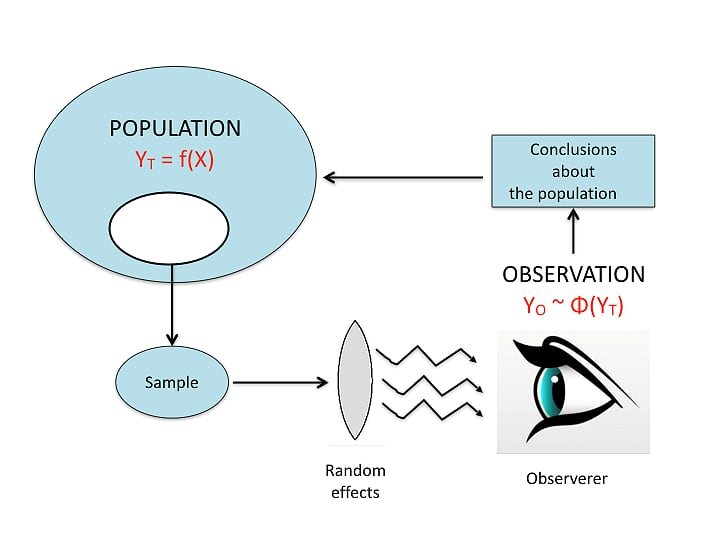
\includegraphics[width=0.75\linewidth]{_images/InferenceProcess} 

}

\caption{Osservazioni sperimentali e meccanismi perturbativi}\label{fig:figName61}
\end{figure}

In questo percorso logico ci sono due aspetti fondamentali che debbono
essere attentamente valutati:

\begin{enumerate}
\def\labelenumi{\arabic{enumi}.}
\tightlist
\item
  modello di generazione dei dati sperimentali;
\item
  sampling distribution (o sample space).
\end{enumerate}

Chiariamo i due concetti con un esempio.

\section{Esempio: una soluzione
erbicida}\label{esempio-una-soluzione-erbicida}

Immaginiamo questa situazione: abbiamo una soluzione erbicida a
concentrazione pari a 120 \(mg/l\), che viene misurata tramite un
gascromatografo. Lo strumento di misura, unitamente a tutte le altre
fonti ignote di errore, produce un coefficiente di variabilità del 10\%
(corrispondete ad una deviazione standard pari a 12 \(mg/l\)). Facciamo
le analisi in triplicato, come usuale per questo tipo di lavori.

\subsection{Il modello dei dati}\label{il-modello-dei-dati}

In primo luogo, ci chiediamo quale sia il modello matematico che genera
le nostre osservazioni. Considerando quanto detto nel capitolo
precedente, possiamo assumere che:

\[ Y_i = \mu + \varepsilon_i\]

dove:

\[ \varepsilon_i \sim N(\mu, \sigma)\]

cioè possiamo assumere che i risultati delle nostre misure siano
normalmente distribuiti con media \(\mu = 120\) e deviazione standard
\(\sigma = 12\).

Con queste informazioni possiamo simulare un esperimento con R,
ottenendo i seguenti risultati:

\begin{Shaded}
\begin{Highlighting}[]
\KeywordTok{set.seed}\NormalTok{(}\DecValTok{1234}\NormalTok{)}
\NormalTok{Y <-}\StringTok{ }\KeywordTok{rnorm}\NormalTok{(}\DecValTok{3}\NormalTok{, }\DecValTok{120}\NormalTok{, }\DecValTok{12}\NormalTok{)}
\NormalTok{Y}
\NormalTok{## [1] 125.1584 114.7349 105.6998}
\end{Highlighting}
\end{Shaded}

\subsection{Analisi dei dati: stima dei
parametri}\label{analisi-dei-dati-stima-dei-parametri}

Nelle due equazioni sovrastanti, gli elementi incogniti sono \(\mu\) e
\(\sigma\). In realtà, dato che si tratta di una simulazione, sappiamo
che essi sono pari, rispettivamente, a 120 e 12; tuttavia, nella realtà
questa informazione sarebbe totalmente sconosciuta. Guardando il
campione, le nostre migliori stime \(\mu\) e \(\sigma\), che chiameremo
rispettivamente \(m\) ed \(s\), sono pari rispettivamente alla media e
alla deviazione standard del campione.

\begin{Shaded}
\begin{Highlighting}[]
\NormalTok{m <-}\StringTok{ }\KeywordTok{mean}\NormalTok{(Y)}
\NormalTok{s <-}\StringTok{ }\KeywordTok{sd}\NormalTok{(Y)}
\NormalTok{m; s}
\NormalTok{## [1] 115.1977}
\NormalTok{## [1] 9.737554}
\end{Highlighting}
\end{Shaded}

Questo processo con il quale assegniamo alla popolazione le
caratteristiche del campione prende il nome di \textbf{stima puntuale}
dei parametri. Vediamo ancora una volta che l'osservazione sperimentale
non coincide con la verità `vera' (\(m \ne \mu\) e \(s \ne \sigma)\), ma
non siamo molto distanti, considerando il 10\% di variabilità dello
strumento di analisi. Tuttavia, visto che dobbiamo trarre conclusioni
che riguardano la popolazione e non il campione, è giustificato da parte
nostra un atteggiamento prudenziale: prima di dire che la concentrazione
erbicida nella soluzione è pari 115.1976637, dobbiamo chiederci: che
cosa succederebbe se ripetessimo l'esperimento molte altre volte?

\subsection{\texorpdfstring{La `sampling
distribution'}{La sampling distribution}}\label{la-sampling-distribution}

In questo caso l'esperimento è solo `elettronico' e possiamo quindi
ripeterlo un numero anche molto elevato di volte, seguendo questa
procedura:

\begin{enumerate}
\def\labelenumi{\arabic{enumi}.}
\tightlist
\item
  Ripetiamo l'estrazione precedente per 100'000 volte (ripetiamo
  l'analisi chimica per 100'000 volte, sempre con tre repliche)
\item
  Otteniamo 100'000 medie
\item
  Calcoliamo la media delle medie e la deviazione standard delle medie
\end{enumerate}

\begin{Shaded}
\begin{Highlighting}[]
\CommentTok{# Simulazione MONTE CARLO - Esempio 1}
\KeywordTok{set.seed}\NormalTok{(}\DecValTok{1234}\NormalTok{)}
\NormalTok{result <-}\StringTok{ }\KeywordTok{rep}\NormalTok{(}\DecValTok{0}\NormalTok{, }\DecValTok{100000}\NormalTok{)}
\ControlFlowTok{for}\NormalTok{ (i }\ControlFlowTok{in} \DecValTok{1}\OperatorTok{:}\DecValTok{100000}\NormalTok{)\{}
\NormalTok{  sample <-}\StringTok{ }\KeywordTok{rnorm}\NormalTok{(}\DecValTok{3}\NormalTok{, }\DecValTok{120}\NormalTok{, }\DecValTok{12}\NormalTok{)}
\NormalTok{  result[i] <-}\StringTok{ }\KeywordTok{mean}\NormalTok{(sample)}
\NormalTok{\}}
\KeywordTok{mean}\NormalTok{(result)}
\NormalTok{## [1] 119.9882}
\KeywordTok{sd}\NormalTok{(result)}
\NormalTok{## [1] 6.924185}
\end{Highlighting}
\end{Shaded}

In sostanza, la simulazione Monte Carlo ci consente di fare quello che
dovremmo sempre fare, cioè ripetere l'esperimento un numero di volte
molto elevato, anche se finito (un numero infinito è chiaramente
impossibile!). A questo punto abbiamo in mano una popolazione di medie,
che viene detta \textbf{sampling distribution}, un `oggetto' abbastanza
`teorico', ma fondamentale per la statistica frequentista, perché
caratterizza la variabilità dei risultati di un esperimento, e quindi la
sua riproducibilità.

Notiamo che:

\begin{enumerate}
\def\labelenumi{\arabic{enumi}.}
\tightlist
\item
  La media delle medie è praticamente coincidente con \(\mu\), la verità
  `vera'. Ciò conferma che l'unico modo di ottenere risultati totalmente
  precisi è ripetere infinite volte l'esperimento;
\item
  La deviazione standard delle medie è pari a 6.9241851. Questo valore
  prende il nome di \textbf{errore standard} della media (SEM).
\end{enumerate}

Esploriamo meglio la \emph{sampling distribution}. Con R possiamo
provare a discretizzarla e a riportarla su di un grafico a barre (figura
\ref{fig:figName62} ).

\begin{Shaded}
\begin{Highlighting}[]
\NormalTok{b <-}\StringTok{ }\KeywordTok{seq}\NormalTok{(}\DecValTok{80}\NormalTok{, }\DecValTok{160}\NormalTok{, }\DataTypeTok{by=}\FloatTok{2.5}\NormalTok{)}
\KeywordTok{hist}\NormalTok{(result, }\DataTypeTok{breaks =}\NormalTok{ b, }\DataTypeTok{freq=}\NormalTok{F, }\DataTypeTok{xlab =} \KeywordTok{expression}\NormalTok{(}\KeywordTok{paste}\NormalTok{(m)),}
  \DataTypeTok{ylab=}\StringTok{"Density"}\NormalTok{, }\DataTypeTok{main=}\StringTok{""}\NormalTok{)}
\KeywordTok{curve}\NormalTok{(}\KeywordTok{dnorm}\NormalTok{(x, }\DecValTok{120}\NormalTok{, }\FloatTok{6.94}\NormalTok{), }\DataTypeTok{add =} \OtherTok{TRUE}\NormalTok{, }\DataTypeTok{col =} \StringTok{"red"}\NormalTok{)}
\end{Highlighting}
\end{Shaded}

\begin{figure}

{\centering 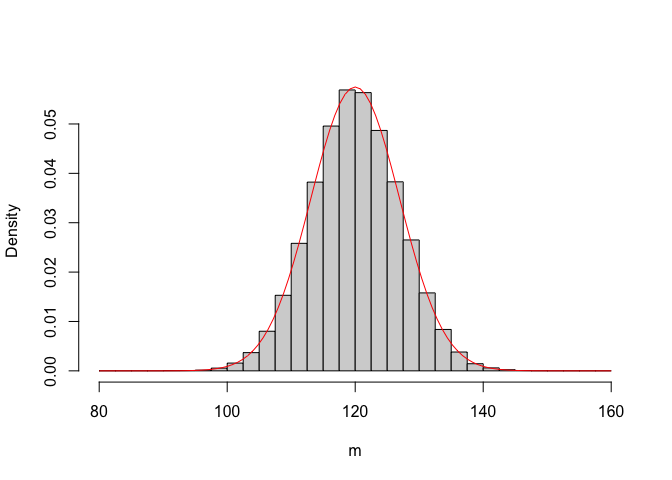
\includegraphics[width=0.9\linewidth]{_main_files/figure-latex/figName62-1} 

}

\caption{Sampling distribution empirica e teorica}\label{fig:figName62}
\end{figure}

\subsection{L'errore standard}\label{lerrore-standard}

La \emph{sampling distribution} che abbiamo ottenuto con la simulazione
Monte Carlo è puramente empirica. Sarebbe interessante capire con più
esattezza se esiste una funzione di densità che permetta di descriverla
con esattezza. In effetti, il grafico precedente mostra che la
\emph{sampling distribution} assomiglia molto ad una distribuzione
normale, con media pari a 120 e deviazione standard pari all'errore
standard.

Formalmente, il problema si può risolvere grazie alla legge di
propagazione degli errori, che stabilisce tre importanti elementi:

\begin{enumerate}
\def\labelenumi{\arabic{enumi}.}
\tightlist
\item
  Se ho due variabili normalmente distribuite e le sommo tra di loro, la
  variabile risultante è ancora normale. Se ho una variabile normalmente
  distribuita e la moltiplico per una costante, la variabile risultante
  è ancora normale.
\item
  Per variabili indipendenti, la varianza della somma è uguale alla
  somma delle varianze.
\item
  La varianza del prodotto di una variabile per una costante \(k\) è
  pari alla varianza della variabile originale moltiplicata per \(k^2\).
\end{enumerate}

Consideriamo che, quando preleviamo alcuni individui da una popolazione,
ognuno di essi porta con sé una sua componente di incertezza, che egli
`eredita' dalla popolazione di cui fa parte. In questo caso, la
popolazione ha una varianza pari a \(12^2 = 144\) e quindi ognuno dei
tre soggetti campionati eredita tale varianza. Quando calcolo la media
di tre osservazioni, in prima battuta io le sommo. A questo punto, dato
che si tratta di osservazioni indipendenti, la propagazione degli errori
(punto 2) ci dice che la varianza della somma è uguale a
\(144 \times 3 = 432\).

Dopo aver sommato, il calcolo della media richiede che il risultato
venga diviso per 3. La legge di propagazione degli errori (punto 3) ci
dice quindi che la varianza viene divisa per \(3^2 = 9\). Insomma la
popolazione delle medie è normale (punto 1), ha media pari a 120 e
varianza pari a \(432/9 = 48\) e, di conseguenza, deviazione standard
pari a \(\sqrt{48} = 6.928\), cioè \(12/\sqrt{3}\). In generale,
l'errore standard di una media è:

\[\sigma_m  = \frac{\sigma }{\sqrt n }\]

dove \emph{n} è la dimensione del campione.

\section{Riepilogo 1: Caratterizzare l'incertezza di un
esperimento}\label{riepilogo-1-caratterizzare-lincertezza-di-un-esperimento}

Che cosa ci insegna questo esperimento? Ci insegna che, se prendiamo una
distribuzione normale con media \(\mu\) e deviazione standard \(\sigma\)
e cominciamo ad estrarre campioni, le medie dei campioni sono variabili,
secondo una distribuzione normale con media \(\mu\) e deviazione
standard \(\sigma / \sqrt{n}\). Questo concetto è interessante e può
essere utilizzato per caratterizzare l'incertezza dei risultati di un
esperimento. Riassumiamo:

\begin{enumerate}
\def\labelenumi{\arabic{enumi}.}
\tightlist
\item
  Abbiamo fatto un esperimento con tre repliche campionando da una
  distribuzione normale incognita.
\item
  Abbiamo ottenuto i tre valori 105.5152, 123.3292 e 133.0133.
\item
  In base alle osservazioni in nostro possesso, concludiamo che la
  concentrazione erbicida è pari a m = 120.6192 \(mg/l\), con una
  deviazione standard pari a 13.9479 \(mg/l\).
\item
  Dobbiamo adottare un atteggiamento prudenziale in relazione alla
  media, dato che non sappiamo il valore vero di \(\mu\).
\item
  Immaginiamo di conoscere la sampling distribution, che avrà una
  deviazione standard pari a:
\end{enumerate}

\begin{Shaded}
\begin{Highlighting}[]
\KeywordTok{sd}\NormalTok{(Y) }\OperatorTok{/}\StringTok{ }\KeywordTok{sqrt}\NormalTok{(}\DecValTok{3}\NormalTok{)}
\NormalTok{## [1] 5.62198}
\end{Highlighting}
\end{Shaded}

\begin{enumerate}
\def\labelenumi{\arabic{enumi}.}
\setcounter{enumi}{5}
\tightlist
\item
  Concludiamo quindi che \(\mu\) è pari a 120.6192 \(\pm\) 8.053
\end{enumerate}

Abbiamo caratterizzato l'incertezza del risultato attraverso un
intervallo di valori (\textbf{stima per intervallo}).

\section{L'intervallo di confidenza}\label{lintervallo-di-confidenza}

Sarebbe interessante poter rispondere a questa domanda: ''qual è la
proporzione di medie (cioè di ipotetici risultati del mio esperimento)
che si trova all'interno della fascia di incertezza data?''. Un passo in
avanti in questo senso è stato fatto da Neyman (1941). Egli ha osservato
che, se guardiamo la \emph{sampling distribution} delle medie
campionarie è possibile isolare due valori simmetrici rispetto a
\(\mu\), che includono al loro interno il 95\% dei possibili risultati
di un esperimento. questi due valori sono:

\begin{Shaded}
\begin{Highlighting}[]
\KeywordTok{qnorm}\NormalTok{(}\FloatTok{0.025}\NormalTok{, }\DecValTok{120}\NormalTok{, }\DecValTok{12}\OperatorTok{/}\KeywordTok{sqrt}\NormalTok{(}\DecValTok{3}\NormalTok{))}
\NormalTok{## [1] 106.421}
\KeywordTok{qnorm}\NormalTok{(}\FloatTok{0.975}\NormalTok{, }\DecValTok{120}\NormalTok{, }\DecValTok{12}\OperatorTok{/}\KeywordTok{sqrt}\NormalTok{(}\DecValTok{3}\NormalTok{))}
\NormalTok{## [1] 133.579}
\end{Highlighting}
\end{Shaded}

Se prendiamo quindi l'intervallo da 106.421 a 133.579 sapppiamo che
resta escluso solo il 5\% dei possibili risultati, cioè quelli di gran
lunga meno probabili. Formalmente potremmo scrivere (uso la notazione R,
per comodità; i dettagli sono nel capitolo precedente):

\[P  \left[ \textrm{qnorm} ( 0.025,\mu,\sigma/\sqrt{n}) \leq m \leq \textrm{qnorm}(0.975,\mu,\sigma/\sqrt{n} ) \right] = 0.95\]

cioè: esiste una probabilità pari a 0.95 che \(m\) sia compreso tra il
2.5-esimo e il 97.5-esimo percentile di una distribuzione normale con
media \(\mu\) e deviazione standard \(\sigma/\sqrt{n}\). In realtà,
invece che lavorare con \(m\), Neyman propose di lavorare con una
statistica diversa, cioè:

\[T = \frac{m - \mu}{\sigma_m}\]

dove \(\sigma_m\) è l'errore standard \(\sigma / \sqrt{n}\). Se \(m\) è
distribuito normalmente con media \(\mu\) e deviazione standard
\(\sigma\), la legge di propagazione degli errori ci dice che T è
distribuito normalmente con media pari a \(m - \mu = 0\) e deviazione
standard \(\sigma_m/\sigma_m = 1\). Cioè la \emph{sampling distribution}
di T è una distribuzione normale standardizzata, con media 0 e
deviazione standard 1.\footnote{Tra tutte le distribuzioni normali, ce
  n'è una particolare, che ha media 0 e deviazione standard 1. Questa si
  chiama \textbf{distribuzione normale standardizzata}}

Quindi possiamo scrivere (si deduce facilmente dall'espressione
precedente):

\[ P \left[ \textrm{qnorm}(0.025, 0, 1) \le \frac{m - \mu }{\sigma_m} \le \textrm{qnorm}(0.975, 0, 1) \right] = 0.95 \]

cioè: esiste una probabilità pari a 0.95 che \(T = (m - \mu)/\sigma_m\)
è compreso tra il 2.5-esimo e il 97.5-esimo percentile di una
distribuzione normale standardizzata. E' facile vedere che:

\begin{Shaded}
\begin{Highlighting}[]
\KeywordTok{qnorm}\NormalTok{(}\FloatTok{0.025}\NormalTok{, }\DecValTok{0}\NormalTok{, }\DecValTok{1}\NormalTok{)}
\NormalTok{## [1] -1.959964}
\KeywordTok{qnorm}\NormalTok{(}\FloatTok{0.975}\NormalTok{, }\DecValTok{0}\NormalTok{, }\DecValTok{1}\NormalTok{)}
\NormalTok{## [1] 1.959964}
\end{Highlighting}
\end{Shaded}

Quindi, approssimando alla seconda cifra decimale:

\[P \left[ -1.96 \le \frac{m - \mu }{\sigma_m} \le 1.96 \right] = 0.95\]

Con semplici passaggi algebrici, possiamo ottenere l'intervallo di
confidenza:

\[P \left[ m -1.96 \times \sigma_m \le \mu \le m + 1.96 \times \sigma_m \right] = 0.95\]

Proviamo a leggere l'espressione sovrastante: \textbf{esiste una
probabilità pari a 0.95 che \(\mu\) (la media vera e ignota della
popolazione), sia compreso all'interno di due valori che si ottengono
sottraendo e aggiungendo alla media del campione \(m\) un multiplo
dell'errore standard. Il coefficiente moltiplicativo è circa pari a
due.}

Il problema è che, nella pratica sperimentale, \(\sigma\) non è noto.
Neyman propose di utilizzare \(s\) al posto di \(\sigma\), cioè la
deviazione standard del campione, invece che quella della popolazione.
Quindi, nel nostro caso, i limiti dell'intervallo di confidenza sono
pari a:

\begin{Shaded}
\begin{Highlighting}[]
\NormalTok{m }\OperatorTok{+}\StringTok{ }\KeywordTok{qnorm}\NormalTok{(}\FloatTok{0.025}\NormalTok{) }\OperatorTok{*}\StringTok{ }\NormalTok{s}\OperatorTok{/}\KeywordTok{sqrt}\NormalTok{(}\DecValTok{3}\NormalTok{)}
\NormalTok{## [1] 104.1788}
\NormalTok{m }\OperatorTok{+}\StringTok{ }\KeywordTok{qnorm}\NormalTok{(}\FloatTok{0.975}\NormalTok{) }\OperatorTok{*}\StringTok{ }\NormalTok{s}\OperatorTok{/}\KeywordTok{sqrt}\NormalTok{(}\DecValTok{3}\NormalTok{)}
\NormalTok{## [1] 126.2165}
\end{Highlighting}
\end{Shaded}

più semplicemente:

\begin{Shaded}
\begin{Highlighting}[]
\NormalTok{m }\OperatorTok{+}\StringTok{ }\DecValTok{2} \OperatorTok{*}\StringTok{ }\NormalTok{s}\OperatorTok{/}\KeywordTok{sqrt}\NormalTok{(}\DecValTok{3}\NormalTok{)}
\NormalTok{## [1] 126.4416}
\NormalTok{m }\OperatorTok{+}\StringTok{ }\DecValTok{2} \OperatorTok{*}\StringTok{ }\NormalTok{s}\OperatorTok{/}\KeywordTok{sqrt}\NormalTok{(}\DecValTok{3}\NormalTok{)}
\NormalTok{## [1] 126.4416}
\end{Highlighting}
\end{Shaded}

Questo che abbiamo calcolato è l'intervallo di confidenza per P = 0.95.
Aumentando opportunamente il moltiplicatore possiamo calcolare gli
intervalli di confidenza per P = 0.99, P = 0.999 e così via. Di fatto,
l'intervallo di confidenza per P = 0.95 è il più utilizzato in pratica.

\section{Qual è il senso dell'intervallo di
confidenza?}\label{qual-e-il-senso-dellintervallo-di-confidenza}

E' utile ricordare il nostro punto di partenza e il nostro punto di
arrivo:

\begin{enumerate}
\def\labelenumi{\arabic{enumi}.}
\tightlist
\item
  PUNTO DI PARTENZA: una distribuzione normale con \(\mu\) = 120 e
  \(\sigma\) = 12. Nella realtà assumiamo che la distribuzione di
  partenza sia normale, mentre i suoi parametri sono totalmente ignoti.
\item
  PUNTO DI ARRIVO: una stima di \(\mu\) ed un intervallo di confidenza.
\end{enumerate}

Che cosa significa questo intervallo? Esso fornisce:

\begin{enumerate}
\def\labelenumi{\arabic{enumi}.}
\tightlist
\item
  una misura di precisione: più piccolo è l'intervallo, maggiore è la
  precisione della stima;
\item
  un'espressione di confidenza nel fatto che, se ripetessimo molte volte
  l'esperimento, nel 95\% dei casi l'intervallo calcolato conterrebbe
  \(\mu\).
\end{enumerate}

Insomma, l'intervallo di confidenza serve ad esplicitare la nostra
incertezza sulla media vera della popolazione in studio.

\section{Come presentare i risultati degli
esperimenti}\label{come-presentare-i-risultati-degli-esperimenti}

Dopo aver letto questo capitolo e quelli precedenti, dovrebbe essere
chiaro che la presenza dell'errore sperimentale crea incertezza in
relazione alle caratteristiche della popolazione da cui abbiamo estratto
il campione. Pertanto, è sempre obbligatorio associare alle nostre stime
un indicatore di incertezza, la cui assenza non è, in linea di
principio, accettabile. Possiamo considerare le seguenti possibilità:

\begin{enumerate}
\def\labelenumi{\arabic{enumi}.}
\tightlist
\item
  riportare la media associata alla deviazione standard, per descrivere
  la variabilità originale del fenomeno in studio;
\item
  riportare la media associata all'errore standard, per descrivere
  l'incertezza associata alla stima della media;
\item
  riportare l'intervallo di confidenza ottenuto sottraendo/aggiungendo
  alla media il doppio dell'errore standard, per descrivere l'incertezza
  associata alla stima della media;
\end{enumerate}

\section{Alcune precisazioni}\label{alcune-precisazioni}

\subsection{Campioni numerosi e non}\label{campioni-numerosi-e-non}

Calcolare l'intervallo di confidenza utilizzando il doppio dell'errore
standard costituisce un'approssimazione che è valida solo quando abbiamo
esperimenti con un numero elevato di soggetti (maggiore di 15-20 circa).
Per gli esperimenti piccoli, è necessario incrementare opportunamente il
moltiplicatore. A questo fine viene utilizzato il valore corrispondente
al 97.5-esimo percentile della distribuzione t di Student (non alla
normale standardizzata, come abbiamo fatto finora), con un numero di
gradi di libertà pari a quelli del campione studiato. Con tre soggetti
il moltiplicatore sarebbe:

\begin{Shaded}
\begin{Highlighting}[]
\KeywordTok{qt}\NormalTok{(}\FloatTok{0.975}\NormalTok{, }\DecValTok{2}\NormalTok{)}
\NormalTok{## [1] 4.302653}
\end{Highlighting}
\end{Shaded}

Il moltiplicatore diminuisce all'aumentare della numerosità e, con 20
soggetti, diviene molto vicino a 2.

\begin{Shaded}
\begin{Highlighting}[]
\KeywordTok{qt}\NormalTok{(}\FloatTok{0.975}\NormalTok{, }\DecValTok{20}\NormalTok{)}
\NormalTok{## [1] 2.085963}
\end{Highlighting}
\end{Shaded}

Nel nostro esempio, con tre soggetti, l'intervallo di confidenza
sarebbe:

\begin{Shaded}
\begin{Highlighting}[]
\NormalTok{m }\OperatorTok{+}\StringTok{ }\KeywordTok{qt}\NormalTok{(}\FloatTok{0.025}\NormalTok{, }\DecValTok{2}\NormalTok{) }\OperatorTok{*}\StringTok{ }\NormalTok{s}\OperatorTok{/}\KeywordTok{sqrt}\NormalTok{(}\DecValTok{3}\NormalTok{)}
\NormalTok{## [1] 91.00824}
\NormalTok{m }\OperatorTok{+}\StringTok{ }\KeywordTok{qt}\NormalTok{(}\FloatTok{0.975}\NormalTok{, }\DecValTok{2}\NormalTok{) }\OperatorTok{*}\StringTok{ }\NormalTok{s}\OperatorTok{/}\KeywordTok{sqrt}\NormalTok{(}\DecValTok{3}\NormalTok{)}
\NormalTok{## [1] 139.3871}
\end{Highlighting}
\end{Shaded}

Quindi, ben più alto di quello approssimato calcolato in precedenza.

\subsection{Popolazioni gaussiane e
non}\label{popolazioni-gaussiane-e-non}

In questo esempio siamo partiti da una popolazione con distribuzione
gaussiana. In altri casi potrebbe non essere così. Ad esempio,
immaginiamo di avere una popolazione di insetti, nella quale il rapporto
tra maschi e femmine è ignoto. Campioniamo 40 insetti e contiamo 15
femmine. Qual è la proporzione di femmine nella popolazione originaria?

In questo caso stiamo studiando una grandezza che, almeno nel principio,
non può essere gaussiana, ma è binomiale (vedi il capitolo precedente).
Nonostante questo, possiamo utilizzare la stessa tecnica per la stima
dell'intervallo di confidenza: sappiamo che la media di una
distribuzione binomiale è \(p = 14/40 = 0.375\), mentre la deviazione
standard è
\(\sigma = \sqrt{0.375 \times (1 - 0.375)} = 0.484\)..\footnote{La
  distribuzione binomiale è trattata in appendice} Di conseguenza,
l'errore standard è \(0.484 / \sqrt{40} = 0.077\). L'intervallo di
confidenza sarà dato quindi da:

\begin{Shaded}
\begin{Highlighting}[]
\FloatTok{0.375} \OperatorTok{-}\StringTok{ }\DecValTok{2} \OperatorTok{*}\StringTok{ }\FloatTok{0.077}
\NormalTok{## [1] 0.221}
\FloatTok{0.375} \OperatorTok{+}\StringTok{ }\DecValTok{2} \OperatorTok{*}\StringTok{ }\FloatTok{0.077}
\NormalTok{## [1] 0.529}
\end{Highlighting}
\end{Shaded}

Chi fosse interessato ad approfondire questi aspetti può proseguire
nella lettura, dopo gli esercizio. Gli altri potranno fermarsi agli
esercizi sottostanti.

\section{Analisi statistica dei dati: riassunto del percorso
logico}\label{analisi-statistica-dei-dati-riassunto-del-percorso-logico}

Considerando quanto finora detto, possiamo riassumere la logica
dell'inferenza tradizionale nel modo seguente:

\begin{enumerate}
\def\labelenumi{\arabic{enumi}.}
\tightlist
\item
  Un esperimento è solo un campione di un numero infinito di esperimenti
  simili che avremmo potuto/dovuto eseguire, ma che non abbiamo
  eseguito, per mancanza di risorse;
\item
  Assumiamo che i dati del nostro esperimento sono generati da un
  modello matematico probabilistico, che prende una certa forma
  algebrica e ne stimiamo i parametri utilizzando i dati osservati;
\item
  Costruiamo la sampling distribution per i parametri stimati o per
  altre statistiche rilevanti, in modo da caratterizzare i risultati
  delle infinite repliche del nostro esperimento, che avremmo dovuto
  fare, ma che non abbiamo fatto.
\item
  Utilizziamo la sampling distribution per l'inferenza statistica.
\end{enumerate}

\section{Da ricordare}\label{da-ricordare}

\begin{enumerate}
\def\labelenumi{\arabic{enumi}.}
\tightlist
\item
  La natura genera i dati
\item
  Noi scegliamo un modello deterministico che simula il meccanismo di
  generazione dei dati attuato dalla natura.
\item
  Stimiamo i parametri.
\item
  Confrontiamo le previsioni con i dati osservati. Determiniamo
  \(\epsilon\) e la sua deviazione standard (\(\sigma\))
\item
  Assumiamo un modello stocastico ragionevole per spiegare \(\epsilon\),
  quasi sempre di tipo gaussiano, con media 0 e deviazione standard pari
  a \(\sigma\), indipendente dalla X (omoscedasticità)
\item
  Qualunque stima sperimentale deve essere associata ad un indicatore di
  variabilità (errore standard o intervallo di confidenza).
\end{enumerate}

\section{Esercizi}\label{esercizi}

\begin{enumerate}
\def\labelenumi{\arabic{enumi}.}
\tightlist
\item
  Un'analisi chimica è stata eseguita in triplicato, ottenendo i
  seguenti risultati: 125, 169 e 142 ng/g. Calcolare media, devianza,
  varianza, deviazione standard, coefficiente di variabilità ed errore
  standard.
\item
  Considerare il campione composto dai valori 140 - 170 - 155 e stimare
  i limiti di confidenza della media (P = 0.95).
\item
  Un campione di 400 insetti a cui è stato somministrato un certo
  insetticida mostra che 136 di essi sono sopravvissuti. Determinare un
  intervallo di confidenza con grado di fiducia del 95\% per la
  proporzione della popolazione insensibile al trattamento.
\end{enumerate}

\chapter{Breve introduzione al test
d'ipotesi}\label{breve-introduzione-al-test-dipotesi}

Nel capitolo precedente abbiamo visto come la \emph{sampling
distribution} (o \emph{sample space} o \emph{distribuzione campionaria})
può essere utilizzata per l'inferenza statistica (stima per intervallo).
Analogamente, essa può essere utilizzata per il test d'ipotesi. Anche in
questo caso, vediamo alcuni esempi, partendo da quello esposto nel
capitolo precedente.

\section{Confronto tra una media osservata e una media
teorica}\label{confronto-tra-una-media-osservata-e-una-media-teorica}

Nel capitolo precedente, abbiamo misurato la concentrazione di una
soluzione erbicida tramite un gascromatografo. Facendo l'analisi in
triplicato, abbiamo ottenuto i tre valori riportati di seguito.

\begin{verbatim}
## [1] 125.1584 114.7349 105.6998
\end{verbatim}

Abbiamo calcolato la media, la deviazione standard, l'errore standard e
l'intervallo di confidenza. Ora immaginiamo che esista un livello soglia
pari a 200 mg/l, al disopra del quale il prodotto diviene tossico per i
mammiferi. Dato che non conosciamo il vero valore di \(\mu\) ci
chiediamo: \emph{è possibile che le nostre tre repliche, nella realtà,
provengano da una popolazione che ha media uguale a 200}?

In questo caso sappiamo bene che non è possibile, visto che abbiamo
generato i dati sperimentali (vedi il capitolo precedente), tramite
simulazione Monte Carlo, partendo da una verità vera nota (\(\mu\) = 120
e \(\sigma\) = 12); tuttavia, nella realtà, la domanda è lecita.

In particolare, possiamo calcolare una statistica, che abbiamo già
utilizzato per l'intervallo di confidenza, in grado di misurare la
discrepanza tra quanto abbiamo osservato e l'ipotesi nulla:

\[ T = \frac{m - 200}{s_m} \]

Il valore da noi osservato è:

\begin{Shaded}
\begin{Highlighting}[]
\NormalTok{T <-}\StringTok{ }\NormalTok{(m }\OperatorTok{-}\StringTok{ }\DecValTok{200}\NormalTok{)}\OperatorTok{/}\NormalTok{sm}
\NormalTok{T}
\NormalTok{## [1] -15.08407}
\end{Highlighting}
\end{Shaded}

il che implica un certo grado di discrepanza, altrimenti avremmo dovuto
osservare un valore di T più vicino a 0. \textbf{Possiamo affermare che
ciò sia imputabile solo alla variabilità di campionamento e che quindi
il nostro esperimento conferma l'ipotesi di partenza (\(\mu = 200\))}?

Definiamo quindi la nostra ipotesi di lavoro come \textbf{ipotesi nulla}
(\(H_0\)):

\[H_0: \mu = 200\]

oppure, che è anche meglio:

\[H_0: T = 0\]

Oltre all'ipotesi nulla, dobbiamo anche definire l'ipotesi alternativa
semplice (a `due code'), che potrebbe essere:

\[H_1: T \neq 0\]

E'possibile anche definire ipotesi alternative complesse del tipo:

\[H_1: T \leq 0\]

oppure:

\[H_1: T \geq 0\]

Bisogna ricordare che le ipotesi debbono essere stabilite prima di
effettuare l'esperimento. In questo caso abbiamo fatto un campionamento
e abbiamo trovato un valore (115.198) inferiore a quello atteso (200).
Che cosa ci attendevamo prima di fare l'esperimento? Un valore diverso
da 200, senza poter lecitamente immaginare se sarebbe stato maggiore o
minore? In questo caso l'ipotesi alternativa dovrebbe essere la prima
(quella semplice). Avevamo invece ragionevoli motivi per ritenere che
\(m\) avrebbe potuto essere inferiore, ma non superiore? In questo caso
l'ipotesi alternativo potrebbe essere la seconda (ipotesi alternativa
complessa). Propendiamo per quest'ultima ipotesi, cioè \(\mu \leq 200\).

Siamo in totale coerenza con la logica Galileiana: abbiamo un ipotesi di
partenza e un esperimento, col quale eventualmente rigettare questa
ipotesi. Fisher, negli anni 20 del 1900, propose di utilizzare come
\textbf{`forza dell'evidenza scientifica' la probabilità di ottenere un
risultato uguale o più estremo di quello osservato, calcolata supponendo
vera l'ipotesi nulla.} Si tratta quindi di capire, tramite la
definizione di un'apposita `sampling distribution' per T, qual è la
proporzione di valori pari o inferiori a -15.084. Per rispondere
utilizzeremo la doppia strada: quella empirica (simulazione Monte Carlo)
e quella formale.

\subsection{Simulazione Monte Carlo}\label{simulazione-monte-carlo}

Ci chiediamo: come sarebbe la \emph{sampling distribution} di T, se
\(\mu\) fosse uguale a 200? Possiamo costruirla con una simulazione
Monte Carlo, ripetendo molte volte (es. 100'000) l'estrazione di
campioni con numerosità pari a 3, da una distribuzione normale con media
pari a 200 e deviazione standard pari a 9.738 e calcolando la statistica
T. Utilizziamo questo valore di deviazione standard perché è quello
osservato nel campione e, nella realtà, sarebbe l'unico valore
disponibile, dato che non sapremmo nulla della popolazione originale.
Per eseguire questa operazione utilizziamo il seguente codice R:

\begin{Shaded}
\begin{Highlighting}[]
\KeywordTok{set.seed}\NormalTok{(}\DecValTok{1234}\NormalTok{)}
\NormalTok{result <-}\StringTok{ }\KeywordTok{rep}\NormalTok{(}\DecValTok{0}\NormalTok{, }\DecValTok{100000}\NormalTok{)}
\ControlFlowTok{for}\NormalTok{ (i }\ControlFlowTok{in} \DecValTok{1}\OperatorTok{:}\DecValTok{100000}\NormalTok{)\{}
\NormalTok{  sample <-}\StringTok{ }\KeywordTok{rnorm}\NormalTok{(}\DecValTok{3}\NormalTok{, }\DecValTok{200}\NormalTok{, s)}
\NormalTok{  result[i] <-}\StringTok{ }\NormalTok{(}\KeywordTok{mean}\NormalTok{(sample) }\OperatorTok{-}\StringTok{ }\DecValTok{200}\NormalTok{) }\OperatorTok{/}\StringTok{ }\NormalTok{(}\KeywordTok{sd}\NormalTok{(sample)}\OperatorTok{/}\KeywordTok{sqrt}\NormalTok{(}\DecValTok{3}\NormalTok{))}
\NormalTok{\}}
\end{Highlighting}
\end{Shaded}

In questo modo otteniamo 100'000 valori di T e possiamo calcolare la
proporzione di questi che è pari o inferiore al valore da noi osservato
(-15.084):

\begin{Shaded}
\begin{Highlighting}[]
\NormalTok{pLev <-}\StringTok{ }\KeywordTok{length}\NormalTok{(result[result }\OperatorTok{<}\StringTok{ }\NormalTok{T])}\OperatorTok{/}\DecValTok{100000}
\NormalTok{pLev}
\NormalTok{## [1] 0.0021}
\end{Highlighting}
\end{Shaded}

Eseguendo questa simulazione, otteniamo una proporzione di valori pari a
0.0021. Il risultato si riassume dicendo che il P-level per l'ipotesi
nulla è pari a 0.0021. La regola di condotta della statistica
tradizionale è quella di rigettare l'ipotesi nulla quando il P-level è
inferiore ad una certa soglia prefissata (normalmente P \(\leq\) 0.05).
Di conseguenza, concludiamo che vi sono elementi sufficienti per
rifiutare l'ipotesi che il valore incognito della concentrazione di
erbicida sia pari a 200 mg/l.

In altre parole, l'evidenza scientifica è sufficiente buona per il
rifiuto dell'ipotesi nulla, anche se esiste una certa probabilità
d'errore, pari appunto alla probabilità che l'ipotesi nulla sia vera (P
= 0.0021).

\subsection{Soluzione formale}\label{soluzione-formale}

Possiamo definire una distribuzione di frequenze per T? Empiricamente
possiamo osservare che, analogamente al caso degli intervalli di
confidenza, la distribuzione di riferimento non è normale, bensì t di
Student, con due gradi di libertà.

\begin{Shaded}
\begin{Highlighting}[]
\CommentTok{#Sampling distribution per T }
\KeywordTok{max}\NormalTok{(result);}\KeywordTok{min}\NormalTok{(result)}
\NormalTok{## [1] 195.249}
\NormalTok{## [1] -169.5243}
\NormalTok{b <-}\StringTok{ }\KeywordTok{seq}\NormalTok{(}\OperatorTok{-}\DecValTok{200}\NormalTok{, }\DecValTok{200}\NormalTok{, }\DataTypeTok{by=}\FloatTok{0.25}\NormalTok{)}
\KeywordTok{hist}\NormalTok{(result, }\DataTypeTok{breaks =}\NormalTok{ b, }\DataTypeTok{freq=}\NormalTok{F, }
  \DataTypeTok{xlab =} \KeywordTok{expression}\NormalTok{(}\KeywordTok{paste}\NormalTok{(m)), }\DataTypeTok{ylab=}\StringTok{"Density"}\NormalTok{, }
  \DataTypeTok{xlim=}\KeywordTok{c}\NormalTok{(}\OperatorTok{-}\DecValTok{10}\NormalTok{,}\DecValTok{10}\NormalTok{), }\DataTypeTok{ylim=}\KeywordTok{c}\NormalTok{(}\DecValTok{0}\NormalTok{,}\FloatTok{0.45}\NormalTok{), }\DataTypeTok{main=}\StringTok{""}\NormalTok{)}
\KeywordTok{curve}\NormalTok{(}\KeywordTok{dnorm}\NormalTok{(x), }\DataTypeTok{add=}\OtherTok{TRUE}\NormalTok{, }\DataTypeTok{col=}\StringTok{"blue"}\NormalTok{)}
\KeywordTok{curve}\NormalTok{(}\KeywordTok{dt}\NormalTok{(x, }\DecValTok{2}\NormalTok{), }\DataTypeTok{add=}\OtherTok{TRUE}\NormalTok{, }\DataTypeTok{col=}\StringTok{"red"}\NormalTok{)}
\end{Highlighting}
\end{Shaded}

\begin{figure}

{\centering 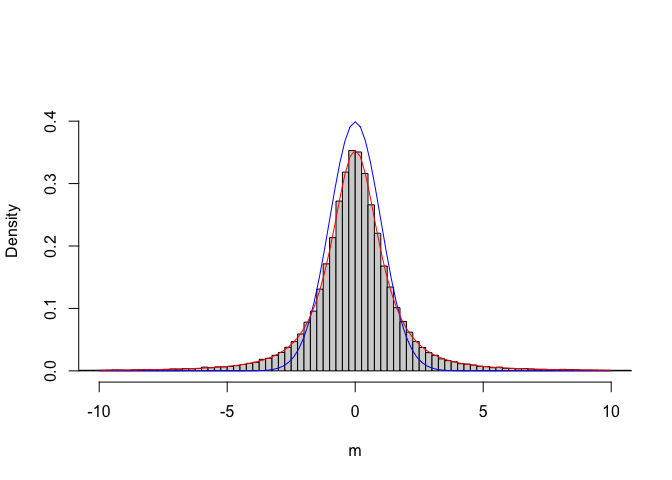
\includegraphics[width=0.85\linewidth]{_main_files/figure-latex/figName71-1} 

}

\caption{Sampling distribution empirica a confronto con una distribuzione normale (in rosso) e una distribuzione t di Student con due gradi di libertà}\label{fig:figName71}
\end{figure}

Senza ricorrere alla simulazione Monte Carlo, possiamo quindi risolvere
il problema utilizzando la distribuzione t di Student, nella quale
cercheremo il valore di probabilità di ottenere valori di T minori o
uguali a quello da noi osservato:

\begin{Shaded}
\begin{Highlighting}[]
\KeywordTok{pt}\NormalTok{(T, }\DataTypeTok{df=}\DecValTok{2}\NormalTok{)}
\NormalTok{## [1] 0.002183138}
\end{Highlighting}
\end{Shaded}

dove gli argomenti indicano rispettivamente il valore osservato. Il
P-level è molto simile a quello ottenuto con la simulazione Monte Carlo.

Allo stesso valore, più semplicemente, si giunge utilizzando la funzione
``t.test()'':

\begin{Shaded}
\begin{Highlighting}[]
\KeywordTok{t.test}\NormalTok{(Y, }\DataTypeTok{mu=}\DecValTok{200}\NormalTok{, }\DataTypeTok{alternative=}\StringTok{"less"}\NormalTok{)}
\NormalTok{## }
\NormalTok{##  One Sample t-test}
\NormalTok{## }
\NormalTok{## data:  Y}
\NormalTok{## t = -15.084, df = 2, p-value = 0.002183}
\NormalTok{## alternative hypothesis: true mean is less than 200}
\NormalTok{## 95 percent confidence interval:}
\NormalTok{##      -Inf 131.6138}
\NormalTok{## sample estimates:}
\NormalTok{## mean of x }
\NormalTok{##  115.1977}
\end{Highlighting}
\end{Shaded}

\subsection{Interpretazione del
P-level}\label{interpretazione-del-p-level}

Quando il P-level è inferiore a 0.05, rifiutiamo l'ipotesi nulla e
concludiamo che vi sono elementi sufficienti (prove scientifiche
sufficientemente forti) per rifiutare la nostra ipotesi di partenza.

Bisogna sottolineare come il P-level nella statistica tradizionale sia
stato inizialmente proposto da Fisher come criterio di comportamento e
non come un vero e proprio criterio inferenziale-probabilistico.
Successivamente, Jarzy Neyman ed Egon Pearson, intorno al 1930,
proposero di utilizzare il P-level come probabilità di errore di I
specie, cioè come probabilità di rifiutare erroneamente l'ipotesi nulla.
Tuttavia, trattandosi di una probabilità calcolata a partire da una
\emph{sampling distribution}, cioè da un'ipotetica infinita ripetizione
dell'esperimento, essa non ha alcun valore in relazione al singolo
esperimento effettivamente eseguito, come i due autori menzionati in
precedenza hanno esplicitamente chiarito.

Di conseguenza, nel caso in esempio, affermare che abbiamo una
probabilità di errore pari a 0.0051 nel rifiutare l'ipotesi nulla,
rappresenterebbe un abuso: le nostre conclusioni potrebbero essere false
o vere, ma non abbiamo alcun elemento per scegliere tra le due opzioni.
Possiamo solo affermare che, se ripetessimo infinite volte l'esperimento
e se l'ipotesi nulla fosse vera, otterremmo un risultato estremo come il
nostro o più estremo solo in 5 casi (circa) su 1000. In altre parole,
nel lungo periodo, basando le nostre conclusioni sul criterio anzidetto
(rifiuto l'ipotesi nulla se il P-value è inferiore a 0.05) commettiamo
un errore in non più del 5\% dei casi. Insomma, il P-level non può
essere guardato come la probabilità di `falso-positivo' ad ogni singolo
test, ma solo nel lunghissimo periodo.

\section{Confronto tra due medie: il test t di
Student}\label{confronto-tra-due-medie-il-test-t-di-student}

Un ricercatore ha scelto casualmente dieci piante da una popolazione; ne
ha trattate cinque con l'erbicida A e cinque con il placebo P. Alla fine
dell'esperimento ha determinato il peso di ognuna delle dieci piante. E'
evidente che le piante oggetto dell'esperimento sono solo un campione di
quelle possibili, così come è evidente che il peso, come ogni altra
variabile biologica è soggetto ad una certa variabilità naturale, legata
sia a questioni genotipiche che fenotipiche, oltre che ad eventuali
errori casuali di misura.

I risultati sono i seguenti:

A (peso in g): 65 - 68 - 69 - 71 - 78; la media è pari a 70.2, mentre la
deviazione standard è pari a 4.87. L'errore standard è pari a 2.18 e
quindi l'intervallo di confidenza della media è 70.2 \(\pm\) 6.04

P (peso in g): 80 - 81 - 84 - 88 - 94; la media è 85.4, mentre la
deviazione standard è pari a 5.72. L'errore standard è pari a 2.56,
mentre l'intervallo di confidenza per la media è 85.4 \(\pm\) 7.11

Possiamo affermare che A riduce il peso delle piante trattate,
coerentemente con le aspettative riguardo ad una molecola erbicida? Nel
rispondere a questa domanda bisogna tener presente che i campioni sono
totalmente irrilevanti, dato che il nostro interesse è rivolto alle
popolazioni che hanno generato i campioni. Vogliamo cioè che le nostre
conclusioni abbiano carattere di universalità e non siano specifiche a
quanto abbiamo osservato nel nostro esperimento. Intanto possiamo notare
che il limite di confidenza superiore per A (70.2 + 6.04 = 76.24) è
inferiore al limite di confidenza inferiore per P (75.4 - 7.11 = 68.29).
Questo non è un criterio sul quale basare le nostre considerazioni, ma è
comunque un segno che le popolazioni da cui provengono i due campioni
potrebbero essere diverse.

Per trovare un criterio decisionali più rigoroso, possiamo formulare
\textbf{l'ipotesi nulla in questi termini}:

\[H_0: \mu_1 = \mu_2 = \mu\]

In altre parole, la nostra ipotesi di lavoro è che i due campioni siano
in realtà estratti da due distribuzioni normali con la stessa media e la
stessa deviazione standard, il che equivale a dire che i due campioni
provengono da un unica distribuzione normale con media \(\mu\) e
deviazione standard \(\sigma\).

L'ipotesi alternativa semplice può essere definita:

\[H_1 :\mu_1  \ne \mu_2\]

Se abbiamo elementi sufficienti già prima di effettuare l'esperimento (e
non dopo aver visto i risultati), possiamo anche adottare ipotesi
alternative complesse, del tipo

\[H_1 :\mu _1  > \mu _2\]

oppure:

\[H_1 :\mu _1  < \mu _2\]

Quale statistica potrebbe meglio descrivere l'andamento
dell'esperimento, in relazione all'ipotesi nulla? E' evidente che questa
statistica dovrebbe essere basata su due indicatori diversi:

\begin{enumerate}
\def\labelenumi{\arabic{enumi}.}
\tightlist
\item
  l'entità della differenza tra le medie: più la differenza tra le due
  medie è alta e più è probabile che essa sia significativa;
\item
  l'entità dell'errore standard. Più è elevata la variabilità dei dati
  (e quindi l'errore di stima) più è bassa la probabilità che le
  differenze osservate tra le medie siano significative.
\end{enumerate}

Su queste basi, si può individuare la seguente statistica:

\[T = \frac{m_1 - m_2}{SED}\]

Si può osservare che T, in realtà, non è altro che il rapporto tra le
quantità indicate in precedenza ai punti 1 e 2: infatti la quantità al
numeratore è la differenza tra le medie dei due campioni, mentre la
quantità al denominatore è il cosiddetto errore standard della
differenza tra due medie (SED). Quest'ultima quantità si può ottenere
pensando che i due campioni sono estratti in modo indipendente e,
pertanto, la varianza della somma (algebrica) è uguale alla somma delle
varianze. La varianza delle due medie è data dal quadrato delle loro
deviazioni standard, cioè dal quadrato degli errori standard (SEM).
Pertanto:

\[SED^2 = SEM_1^2 + SEM_2^2\]

Sappiamo anche che il SEM si ottiene dividendo la deviazione standard di
ogni campione per la radice quadrata del numero dei dati, quindi:

\[SED^2 = \frac{s_1^2}{n_1} +  \frac{s_2^2}{n_2}\]

cioè:

\[SED = \sqrt{ \frac{s_1^2}{n_1} +  \frac{s_2^2}{n_2} }\]

Possiamo anche scrivere:

\[SED = \sqrt{ \frac{s_1^2 \, n_2 + s_2^2 \, n_1}{n_1 \, n_2} }\]

e, se le varianze sono uguali (\(s_1^2 = s_2^2 = s^2\)), segue che:

\[SED = \sqrt {s^2 \frac{n_1  + n_2}{n_1 \, n_2 } }\]

Se fosse anche \(n_1 = n_2 =n\), potremmo scrivere:

\[SED = \sqrt{2 \, \frac{s^2}{n} } = \sqrt{2} \times SEM\]

Il valore osservato per T è quindi uguale a:

\[T = \frac{85.4 - 70.2}{3.361547} = 4.5217\]

dove il denominatore è ottenuto come:

\[SED = \sqrt{ 2.18^2 +  2.56^2 } = 3.361547\]

A questo punto avendo osservato T = 4.5217, possiamo chiederci: qual è
la `sampling distribution' per T, cioè quali valori potrebbe assumere
questa statistica se ripetessimo il campionamento infinite volte,
assumendo che l'ipotesi nulla fosse vera?

La sampling distribution per T potrebbe essere ottenuta empiricamente,
utilizzando una simulazione Monte Carlo. Il codice da utilizzare per
questa simulazione è fornito in appendice, dove si può vedere che,
formalmente, la sampling distribution per T è una distribuzione t di
Student, con 8 gradi di libertà (quattro per campione). Siamo quindi in
grado di calcolare la probabilità di ottenere valori di T altrettanto
estremi o più estremi di quello da noi osservato, tenendo però presente
che il test è `a due code'. Infatti, il T osservato è positivo, ma solo
perché abbiamo scritto la differenza come \(m_2 - m_1\) invece che come
\(m_1 - m_2\). Tuttavia, entrambe le differenze sono possibili, quindi
dobbiamo considerare anche il valore reciproco -T. In altre parole, ci
chiediamo qual è la possibilità di campionare da una distribuzione t di
Student valori esterni all'intervallo (-4.5217; 4.5217). La risposta,
con R, è piuttosto semplice da ottenere:

\begin{Shaded}
\begin{Highlighting}[]
\DecValTok{2} \OperatorTok{*}\StringTok{ }\KeywordTok{pt}\NormalTok{(T, }\DecValTok{8}\NormalTok{, }\DataTypeTok{lower.tail=}\NormalTok{T)}
\NormalTok{## [1] 3.690001e-07}
\end{Highlighting}
\end{Shaded}

Abbiamo moltiplicato per 2 il risultato, in quanto la funzione `dt()'
fornisce la probabilità di trovare individui inferiori a -4.5217
(`lower.tail = T'). Essendo la distribuzione simmetrica, la probabilità
di trovare soggetti superiori a 4.5217 è esattamente la stessa.

Vediamo che il P-level è minore di 0.05 e possiamo quindi rifiutare
l'ipotesi nulla. Concludiamo che vi è un'evidenza scientifica abbastanza
forte per ritenere che l'erbicida A induca una riduzione del peso delle
piante trattate.

Allo stesso valore, più semplicemente, si perviene utilizzando la
funzione:

\begin{Shaded}
\begin{Highlighting}[]
\KeywordTok{t.test}\NormalTok{(A, P, }\DataTypeTok{var.equal=}\NormalTok{T)}
\NormalTok{## }
\NormalTok{##  Two Sample t-test}
\NormalTok{## }
\NormalTok{## data:  A and P}
\NormalTok{## t = -4.5217, df = 8, p-value = 0.001945}
\NormalTok{## alternative hypothesis: true difference in means is not equal to 0}
\NormalTok{## 95 percent confidence interval:}
\NormalTok{##  -22.951742  -7.448258}
\NormalTok{## sample estimates:}
\NormalTok{## mean of x mean of y }
\NormalTok{##      70.2      85.4}
\end{Highlighting}
\end{Shaded}

Gli argomenti della funzione `t.test()' sono i due vettori è l'argomento
`var.equal', che in questo caso è stato settato su TRUE. Per comprendere
il significato di quest'ultimo argomento, dobbiamo sapere che esistono
diversi tipi di test di t. L'argomento è trattato in modo più
dettagliato in appendice, ma è bene sapere che si possono presentare tre
casi diversi:

\begin{enumerate}
\def\labelenumi{\arabic{enumi}.}
\tightlist
\item
  Le misure sono prese su soggetti diversi (indipendenti) e possiamo
  suppore che i due campioni provengano da due popolazioni con la stessa
  varianza (test t omoscedastico).
\item
  Le misure sono prese su soggetti diversi, ma le varianze delle due
  popolazioni non sono ragionevolmente omogenee (test t
  eteroscedastico).
\item
  Le misure sono prese a coppia sullo stesso soggetto e non sono quindi
  indipendenti (test t appaiato).
\end{enumerate}

Nel nostro esempio vediamo che le varianze dei campioni sono piuttosto
simili e quindi adottiamo un test t omoscedastico (`var.equal = T').

Se dovessimo supporre che i due campioni provengono da popolazioni con
varianze diverse, allora dovremmo adottare un test di t
esteroscedastico, con il codice che segue:

\begin{Shaded}
\begin{Highlighting}[]
\KeywordTok{t.test}\NormalTok{(A, P, }\DataTypeTok{var.equal=}\NormalTok{F)}
\NormalTok{## }
\NormalTok{##  Welch Two Sample t-test}
\NormalTok{## }
\NormalTok{## data:  A and P}
\NormalTok{## t = -4.5217, df = 7.7977, p-value = 0.002076}
\NormalTok{## alternative hypothesis: true difference in means is not equal to 0}
\NormalTok{## 95 percent confidence interval:}
\NormalTok{##  -22.986884  -7.413116}
\NormalTok{## sample estimates:}
\NormalTok{## mean of x mean of y }
\NormalTok{##      70.2      85.4}
\end{Highlighting}
\end{Shaded}

Se invece avessimo rilevato le misure accoppiate su quattro individui,
dovremmo utilizzare un test di t appaiato, con il codice seguente:

\begin{Shaded}
\begin{Highlighting}[]
\KeywordTok{t.test}\NormalTok{(A, P, }\DataTypeTok{var.equal=}\NormalTok{T, }\DataTypeTok{paired=}\NormalTok{T)}
\NormalTok{## }
\NormalTok{##  Paired t-test}
\NormalTok{## }
\NormalTok{## data:  A and P}
\NormalTok{## t = -22.915, df = 4, p-value = 2.149e-05}
\NormalTok{## alternative hypothesis: true difference in means is not equal to 0}
\NormalTok{## 95 percent confidence interval:}
\NormalTok{##  -17.04169 -13.35831}
\NormalTok{## sample estimates:}
\NormalTok{## mean of the differences }
\NormalTok{##                   -15.2}
\end{Highlighting}
\end{Shaded}

\section{\texorpdfstring{Confronto tra due proporzioni: il test
\(\chi^2\)}{Confronto tra due proporzioni: il test \textbackslash{}chi\^{}2}}\label{confronto-tra-due-proporzioni-il-test-chi2}

Il test di t è molto utile, ma soltanto nel caso in cui si abbia a che
fare con caratteri quantitativi, cioè con variabili misurate su una
scala continua, per le quali sia possibile calcolare statistiche
descrittive, come appunto la media. Talvolta, i ricercatori sono
interessati a rilevare caratteristiche qualitative, come ad esempio lo
stato di una pianta in seguito ad un trattamento (morta o viva), il
colore dei semi (si ricordino i piselli verdi e gialli di Mendel) ed
altre caratteristiche che non sono misurabili su una scala continua.

Avendo a che fare con variabili qualitative, l'unica statistica
rilevabile è il numero di soggetti che presentano le diverse modalità.
Ad esempio, immaginiamo un esperimento per verificare se un coadiuvante
aumenta l'efficacia di un erbicida. In questo esperimento, utilizziamo
l'erbicida da solo e miscelato con il coadiuvante su due gruppi di
soggetti diversi. Nel primo gruppo (trattato con erbicida) contiamo 56
morti su 75 piante trattate, mentre nel secondo gruppo (trattato con
erbicida e coadiuvante) otteniamo 48 morti su 50 piante trattate.

I risultati di questo esperimento si riducono ad una tabella di
contingenza:

\begin{Shaded}
\begin{Highlighting}[]
\NormalTok{counts <-}\StringTok{ }\KeywordTok{c}\NormalTok{(}\DecValTok{56}\NormalTok{, }\DecValTok{19}\NormalTok{, }\DecValTok{48}\NormalTok{, }\DecValTok{2}\NormalTok{)}
\NormalTok{tab <-}\StringTok{ }\KeywordTok{matrix}\NormalTok{(counts, }\DecValTok{2}\NormalTok{, }\DecValTok{2}\NormalTok{, }\DataTypeTok{byrow =}\NormalTok{ T)}
\KeywordTok{row.names}\NormalTok{(tab) <-}\StringTok{ }\KeywordTok{c}\NormalTok{(}\StringTok{"E"}\NormalTok{, }\StringTok{"EC"}\NormalTok{)}
\KeywordTok{colnames}\NormalTok{(tab) <-}\StringTok{ }\KeywordTok{c}\NormalTok{(}\StringTok{"M"}\NormalTok{, }\StringTok{"V"}\NormalTok{)}
\NormalTok{tab}
\NormalTok{##     M  V}
\NormalTok{## E  56 19}
\NormalTok{## EC 48  2}
\end{Highlighting}
\end{Shaded}

Sappiamo già che, per una tabella di contingenza, possiamo determinare
una statistica che misura la connessione tra variabili (trattamento e
mortalità) connessione, detta \(\chi^2\). La connession è l'indicatore
giusto per rispondere alla nostra domanda di ricerca; infatti ci stiamo
chiedendo se la proporzione dei morti è indipendente dal tipo di
trattamento oppure no.

Sappiamo che, con R, il \(\chi^2\) si calcola applicando la funzione
summary all'oggetto `data.table':

\begin{Shaded}
\begin{Highlighting}[]
\KeywordTok{summary}\NormalTok{( }\KeywordTok{as.table}\NormalTok{(tab) )}
\NormalTok{## Number of cases in table: 125 }
\NormalTok{## Number of factors: 2 }
\NormalTok{## Test for independence of all factors:}
\NormalTok{##  Chisq = 9.768, df = 1, p-value = 0.001776}
\end{Highlighting}
\end{Shaded}

Il valore di \(\chi^2\) osservato è pari a 9.768, il che indica un certo
grado di connessione. Infatti, ricordimao che, in caso di indipendenza
tra le variabili, \(\chi^2\) dovrebbe essere zero. Tuttavia, noi non
siamo interessati ai due campioni, in quanto i 125 soggetti osservati
sono tratti da due popolazioni più ampie. Considerando queste due
popolazioni, poniamo l'ipotesi nulla in questi termini:

\[H_o :\pi_1  = \pi_2  = \pi\]

Vediamo che, come negli altri esempio, l'ipotesi nulla riguarda i
parametri delle popolazioni (\(\pi_1\) e \(\pi_2\)), non quelli dei
campioni (\(p_1\) e \(p_2\)). Ci chiediamo: se l'ipotesi nulla è vera
(\(\pi_1 = \pi_2\)), qual è la sampling distribution per \(\chi^2\)? E
soprattutto, quanto è probabile ottenere un valore alto come il nostro o
più alto?

In appendice mostriamo come si possa arrivare a questo risultato con una
simulazione Monte Carlo. In modo formale, si può dimostrare che, se
\(n\) è sufficientemente grande (n \textgreater{} 30), il valore
osservato di \(\chi^2\) segue appunto la distribuzione di probabilità
\(\chi^2\), con un numero di gradi di libertà \(\nu\) pari al numero dei
dati indipendenti, che, in questo caso, è pari ad 1. Infatti, una volta
fissata una frequenza, le altre sono automaticamente definite, dovendo
restituire i totali marginali. In R, possiamo utilizzare la funzione
`pchi()' per calcolare la probabilità di ottenere valori pari o
superiori a 9.768:

\begin{Shaded}
\begin{Highlighting}[]
\KeywordTok{pchisq}\NormalTok{(}\FloatTok{9.76801}\NormalTok{, }\DecValTok{1}\NormalTok{, }\DataTypeTok{lower.tail=}\NormalTok{F)}
\NormalTok{## [1] 0.001775746}
\end{Highlighting}
\end{Shaded}

Allo stesso risultato, ma in modo più semplice, è possibile pervenire
utilizzando la già citata funzione `summary()', applicata alla tabella
di contingenza (vedi sopra), oppure:

\begin{Shaded}
\begin{Highlighting}[]
\KeywordTok{chisq.test}\NormalTok{(tab, }\DataTypeTok{correct=}\NormalTok{F)}
\NormalTok{## }
\NormalTok{##  Pearson's Chi-squared test}
\NormalTok{## }
\NormalTok{## data:  tab}
\NormalTok{## X-squared = 9.768, df = 1, p-value = 0.001776}
\end{Highlighting}
\end{Shaded}

\section{Conclusioni}\label{conclusioni-1}

Abbiamo visto quale strumento abbiamo a disposizione per tirare
conclusioni in presenza di incertezza sperimentale. Dovrebbe essere
evidente che anche le nostre conclusioni sono incerte, in quanto
soggette all'errore di campionamento. In particolare, abbiamo visto che
esiste un rischio di errore di prima specie, cioè rifiutare erronamente
l'ipotesi nulla (falso positivo). Allo stesso modo, esiste anche un
rischio di errore di II specie, cioè accettare erroneamente l'ipotesi
nulla (falso negativo). Di questi due tipi di errore abbiamo parlato più
diffusamente in appendice.

\section{Riepilogo}\label{riepilogo}

Lo schema di lavoro, nel test d'ipotesi, è il seguente:

\begin{enumerate}
\def\labelenumi{\arabic{enumi}.}
\tightlist
\item
  Si formula l'ipotesi nulla;
\item
  Si individua una statistica che descriva l'andamento dell'esperimento,
  in relazione all'ipotesi nulla;
\item
  Si individua la sampling distribution per questa statistica, assumendo
  vera l'ipotesi nulla; la sampling distribution può essere empirica
  (ottenuta per simulazione) o teorica, scelta in base a considerazioni
  probabilistiche
\item
  Si calcola la probabilità che, essendo vera l'ipotesi nulla, si possa
  osservare una valore altrettanto estremo o più estremo di quello
  calcolato, per la statistica di riferimento;
\item
  Se il livello di probabilità è inferiore ad una certa soglia
  \(\alpha\) prefissata (generalmente 0.05), si rifiuta l'ipotesi nulla.
\end{enumerate}

\section{Esercizi}\label{esercizi-1}

\begin{enumerate}
\def\labelenumi{\arabic{enumi}.}
\tightlist
\item
  Uno sperimentatore ha impostato un esperimento verificare l'effetto di
  un fungicida (A) in confronto al testimone non trattato (B), in base
  al numero di colonie fungine sopravvissute. Il numero delle colonie
  trattate è di 200, con 180 colonie sopravvissute al trattamento. Il
  numero di quelle non trattate è di 100, con 50 colonie sopravvissute.
  Stabilire se i risultati possono essere considerati significativamente
  diversi, per un livello di probabilità del 5\%
\item
  Uno sperimentatore ha impostato un esperimento per confrontare due
  tesi sperimentali (A, B). Per la tesi A sono stati osservate le
  seguenti produzioni: 9.3, 10.2, 9.7. Per la tesi B, sono state
  osservati valori di 12.6, 12.3 e 12.5. Stabilire se i risultati
  possono essere considerati significativamente diversi, per un livello
  di probabilità del 5\%.
\item
  Uno sperimentatore ha impostato un esperimento per confrontare se
  l'effetto di un fungicida è significativo, in un disegno sperimentale
  con tre ripetizioni. Con il trattamento, i risultati produttivi (in
  t/ha) sono 65, 71 e 68. Con il non trattato, i risultati sono 54, 51 e
  59. E'significativo l'effetto del trattamento fungicida sulla
  produzione, per un livello di probabilità di errore del 5\%?
\item
  Immaginate di aver riscontrato che, in determinate condizioni
  ambientali, 60 olive su 75 sono attaccate da \emph{Daucus olee} (mosca
  dell'olivo). Nelle stesse condizioni ambientali, diffondendo in campo
  un insetto predatore siamo riusciti a ridurre il numero di olive
  attaccate a 12 su 75. Si tratta di una oscillazione casuale del
  livello di attacco o possiamo concludere che l'insetto predatore è
  stato un mezzo efficace di lotta biologica alla mosca dell'olivo?
\end{enumerate}

\chapter{Una variabile indipendente categorica: ANOVA ad una
via}\label{una-variabile-indipendente-categorica-anova-ad-una-via}

\section{La situazione sperimentale}\label{la-situazione-sperimentale}

Immaginiamo di aver posto a confronto cinque trattamenti sperimentali
qualitativi (tipi di concime o varietà di frumento o diserbanti) e di
aver registrato il loro effetto su una variabile quantitativa (ad
esempio la produzione). Ci troviamo quindi ad avere un collettivo di
osservazioni, all'interno delle quali esistono gruppi diversi di
soggetti, classificabili in base al trattamento a cui sono stati
sottoposti. Al solito, sappiamo che i soggetti osservati sono solo un
campione di tutti quelli possibili, quindi dietro ai nostri soggetti vi
è almeno una popolazione di riferimento. Più precisamente: se i
trattamenti effettuati non avessero avuto effetto, avremmo una sola
popolazione di riferimento e cinque campioni diversi provenienti dalla
stessa popolazione. Se invece i trattamenti fossero stati efficaci,
allora avremmo cinque popolazioni diverse, per la media, per la
deviazione standard o per entrambe. Per semplicità, assumiamo che le
cinque popolazioni differiscano solo per la media e non per la
deviazione standard.

La prima ipotesi scientifica può essere tradotta in questo modo:

\[ Y_i = \mu + \varepsilon\]

con \(\varepsilon \sim N(0, \sigma)\). Insomma, abbiamo una sola
popolazione distribuita normalmente, con media \(\mu\) e deviazione
standard \(\sigma\). La seconda ipotesi, più interessante da un punto di
vista sperimentale, è questa:

\[Y_i = \mu + \alpha_j + \varepsilon\]

Qui abbiamo un'intercetta \(\mu\) (vedremo tra breve cosa rappresenta),
mentre \(\alpha_j\) è l'effetto del j-esimo trattamento. Per capire cosa
rappresenta \(\mu\) dobbiamo pensare a due trattamenti, la cui media sia
rispettivamente pari a 15 e 25. Se poniamo \(\mu = 20\) (la media
generale), allora \(\alpha_1 = - 5\) e \(\alpha_2 = 5\). Ma è anche vero
che alla stessa soluzione si potrebbe pervenire ponendo \(\mu = 19\) e
quindi \(\alpha_1 = -4\) e \(\alpha_2 = 6\). ugualmente potremmo porre
\(\mu = 18\) e quindi \(\alpha_1 = -3\) e \(\alpha_2 = 7\). E così via.
Insomma, l'equazione lineare sovrastante ha infinite soluzioni.

Per uscire da questo impasse, dobbiamo porre dei vincoli. Ad esempio
potremmo porre il vincolo che \(\alpha_1 = 0\). In questo caso risulta
definito che \(\mu\) deve essere pari alla media del primo trattamento
(\(\mu = 15\)) e \(\alpha_2 = 10\) (vincolo sul trattamento). Oppure
potremmo porre il vincolo che \(\sum{\alpha} = 0\), quindi risulta
definito che \(\mu\) deve essere pari alla media generale (\(\mu = 20\))
e \(\alpha_1 = -5\) (vincolo sulla somma). Un'altra possibilità è
imporre che \(\mu\) sia uguale a 0 (vincolo sull'intercetta).

Questi vincoli prendono il nome di PARAMETRIZZAZIONI del modello
lineare; la prima parametrizzazione (con vincolo sul trattamento) è
quella di default, nella gran parte dei software statistici, incluso R.

\section{\texorpdfstring{La verità `vera' (la
popolazione)}{La verità vera (la popolazione)}}\label{la-verita-vera-la-popolazione}

Immaginiamo che, nella nostra popolazione, le medie dei cinque
trattamenti siano:

\begin{enumerate}
\def\labelenumi{\arabic{enumi}.}
\tightlist
\item
  A = 9
\item
  B = 5
\item
  C = 16
\item
  D = 27
\item
  E = 31
\end{enumerate}

Immaginiamo anche che l'errore sperimentale si gaussiano, con media 0 e
deviazione standard pari a \(\sigma = 1.5\).

Penso sia opportuno ricordare l'elenco delle assunzioni che abbiamo
posto:

\begin{enumerate}
\def\labelenumi{\arabic{enumi}.}
\tightlist
\item
  il modello deterministico è lineare, additivo
\item
  non vi sono altri effetti, se non il trattamento e l'errore (puramente
  stocastico, con media 0 e valori indipendenti)
\item
  gli errori sono normalmente distribuiti
\item
  le varianze sono omogenee (unico valore di \(\sigma\), comune per
  tutti i gruppi)
\end{enumerate}

\section{Esecuzione dell'esperimento}\label{esecuzione-dellesperimento}

Immaginiamo di fare un esperimento con 8 repliche e generiamo i dati con
una simulazione di Monte Carlo.

\begin{Shaded}
\begin{Highlighting}[]
\NormalTok{treat <-}\StringTok{ }\KeywordTok{rep}\NormalTok{(LETTERS[}\DecValTok{1}\OperatorTok{:}\DecValTok{5}\NormalTok{], }\DataTypeTok{each =} \DecValTok{8}\NormalTok{)}
\NormalTok{mu <-}\StringTok{ }\DecValTok{9}\NormalTok{; alpha2 <-}\StringTok{ }\OperatorTok{-}\DecValTok{4}\NormalTok{; alpha3 <-}\StringTok{ }\DecValTok{7}\NormalTok{; alpha4 <-}\StringTok{ }\DecValTok{18}
\NormalTok{alpha5 <-}\StringTok{ }\DecValTok{22}\NormalTok{; sigma <-}\StringTok{ }\FloatTok{1.5}
\NormalTok{alpha <-}\StringTok{ }\KeywordTok{c}\NormalTok{(}\DecValTok{0}\NormalTok{, alpha2, alpha3, alpha4, alpha5)}
\NormalTok{Ye <-}\StringTok{ }\KeywordTok{rep}\NormalTok{(mu }\OperatorTok{+}\StringTok{ }\NormalTok{alpha, }\DataTypeTok{each =} \DecValTok{8}\NormalTok{)}
\KeywordTok{set.seed}\NormalTok{(}\DecValTok{1234}\NormalTok{)}
\NormalTok{Y <-}\StringTok{ }\NormalTok{Ye }\OperatorTok{+}\StringTok{ }\KeywordTok{rnorm}\NormalTok{(}\DecValTok{40}\NormalTok{, }\DecValTok{0}\NormalTok{, sigma)}
\NormalTok{dataset <-}\StringTok{ }\KeywordTok{data.frame}\NormalTok{(}\DataTypeTok{treat =}\NormalTok{ treat, }\DataTypeTok{Y =}\NormalTok{ Y)}
\KeywordTok{rm}\NormalTok{(}\DataTypeTok{list=}\NormalTok{(}\KeywordTok{ls}\NormalTok{()[}\KeywordTok{ls}\NormalTok{()}\OperatorTok{!=}\StringTok{"dataset"}\NormalTok{]))}
\KeywordTok{head}\NormalTok{(dataset)}
\NormalTok{##   treat        Y}
\NormalTok{## 1     A 9.644795}
\NormalTok{## 2     A 8.341859}
\NormalTok{## 3     A 7.212470}
\NormalTok{## 4     A 7.383091}
\NormalTok{## 5     A 8.824202}
\NormalTok{## 6     A 7.903032}
\end{Highlighting}
\end{Shaded}

\section{Analisi dei dati}\label{analisi-dei-dati}

\subsection{Statistiche descrittive}\label{statistiche-descrittive}

Descriviamo la tendenza centrale e la variabilità dei cinque gruppi.

\begin{Shaded}
\begin{Highlighting}[]
\KeywordTok{library}\NormalTok{(plyr)}
\NormalTok{statDesc <-}\StringTok{ }\NormalTok{medie2 <-}\StringTok{ }\KeywordTok{ddply}\NormalTok{(dataset, }\OperatorTok{~}\NormalTok{treat, summarise, }\DataTypeTok{media =} \KeywordTok{mean}\NormalTok{(Y), }\DataTypeTok{devSt =} \KeywordTok{sd}\NormalTok{(Y))}
\NormalTok{statDesc}
\NormalTok{##   treat     media     devSt}
\NormalTok{## 1     A  8.167906 0.8779368}
\NormalTok{## 2     B  5.698595 1.5159899}
\NormalTok{## 3     C 16.280251 1.3902306}
\NormalTok{## 4     D 27.149423 1.7569298}
\NormalTok{## 5     E 30.948257 1.3541870}
\end{Highlighting}
\end{Shaded}

Vediamo che i risultati riflettono abbastanza bene, ma non
perfettamente, le caratteristiche della popolazione.

\subsection{Stima dei parametri}\label{stima-dei-parametri}

In questo caso (disegno bilanciato, con lo stesso numero di repliche per
trattamento), la stima dei parametri potrebbe essere fatta a mano,
abbastanza facilmente. Più in generale, utilizziamo R.

\begin{Shaded}
\begin{Highlighting}[]
\NormalTok{mod <-}\StringTok{ }\KeywordTok{lm}\NormalTok{(Y }\OperatorTok{~}\StringTok{ }\KeywordTok{factor}\NormalTok{(treat), }\DataTypeTok{data =}\NormalTok{ dataset)}
\end{Highlighting}
\end{Shaded}

La specifica del modello è chiara, considerando che l'incusione
dell'intercetta è opzionale (`\textasciitilde{} 1 + treat') è
\(\epsilon\) viene incluso di default. Il termine `factor' sta a
significare che la variabile `treat' è un fattore sperimentale. Questa
specifica è opzionale in questo caso in cui la variabile è di tipo
`carattere', ma è fondamentale quando abbiamo a che fare con una
codifica numerica.

Vediamo ora le stime dei parametri.

\begin{Shaded}
\begin{Highlighting}[]
\KeywordTok{summary}\NormalTok{(mod)}
\NormalTok{## }
\NormalTok{## Call:}
\NormalTok{## lm(formula = Y ~ factor(treat), data = dataset)}
\NormalTok{## }
\NormalTok{## Residuals:}
\NormalTok{##     Min      1Q  Median      3Q     Max }
\NormalTok{## -3.4779 -0.8498 -0.0626  1.0956  2.0180 }
\NormalTok{## }
\NormalTok{## Coefficients:}
\NormalTok{##                Estimate Std. Error t value Pr(>|t|)    }
\NormalTok{## (Intercept)      8.1679     0.4981  16.400  < 2e-16 ***}
\NormalTok{## factor(treat)B  -2.4693     0.7044  -3.506  0.00127 ** }
\NormalTok{## factor(treat)C   8.1123     0.7044  11.517 1.86e-13 ***}
\NormalTok{## factor(treat)D  18.9815     0.7044  26.949  < 2e-16 ***}
\NormalTok{## factor(treat)E  22.7804     0.7044  32.342  < 2e-16 ***}
\NormalTok{## ---}
\NormalTok{## Signif. codes:  0 '***' 0.001 '**' 0.01 '*' 0.05 '.' 0.1 ' ' 1}
\NormalTok{## }
\NormalTok{## Residual standard error: 1.409 on 35 degrees of freedom}
\NormalTok{## Multiple R-squared:  0.983,  Adjusted R-squared:  0.981 }
\NormalTok{## F-statistic: 505.6 on 4 and 35 DF,  p-value: < 2.2e-16}
\end{Highlighting}
\end{Shaded}

Notiamo immediatamente che viene utilizzata la parametrizzazione con
vincolo sul trattamento, visto che l'intercetta coincide con la media
del primo trattamento.

\subsection{Stima della varianza}\label{stima-della-varianza}

Il residuo \(\varepsilon\) rappresenta la componente casuale: se non vi
fosse errore. la prima osservazione dovrebbe avere un valore pari al
valore atteso del gruppo di cui fa parte (8.5543). In realtà essa è pari
a 9.6447955, con un residuo, rispetto all'atteso' pari a 1.0904955.

La serie completa dei residui può essere ottenuta come segue:

\begin{Shaded}
\begin{Highlighting}[]
\NormalTok{epsilon <-}\StringTok{ }\KeywordTok{residuals}\NormalTok{(mod)}
\end{Highlighting}
\end{Shaded}

La devianza del residuo (somma dei quadrati degli scarti) è:

\begin{Shaded}
\begin{Highlighting}[]
\NormalTok{RSS <-}\StringTok{ }\KeywordTok{sum}\NormalTok{( epsilon}\OperatorTok{^}\DecValTok{2}\NormalTok{ )}
\NormalTok{RSS}
\NormalTok{## [1] 69.45655}
\end{Highlighting}
\end{Shaded}

Quanri gradi di libertà ha questa somma? Dobbiamo tener presente che i
residui sono somme di quadrati di scarti rispetto alla media di ogni
trattamento. Di conseguenza, la media dei residui è costretta ad essere
zero per ogni trattamento, il che significa che, sempre per ogni
trattamento, sette scarti sono liberi (7 gradi di libertà), mentre
l'ottavo deve essere tale che sommato con gli altri restituisce zero.
Quindi abbiamo 7 \(\times\) 5 = 35 gradi di libertà. Possiamo quindi
calcolare la deviazione standard del residuo come:

\begin{Shaded}
\begin{Highlighting}[]
\NormalTok{sigma <-}\StringTok{ }\KeywordTok{sqrt}\NormalTok{( RSS}\OperatorTok{/}\DecValTok{35}\NormalTok{ )}
\NormalTok{sigma}
\NormalTok{## [1] 1.408713}
\end{Highlighting}
\end{Shaded}

In realtà, questo valore l'avevamo già visto applicando la funzione
`summary()' all'oggetto `mod'. Da questo valore possiamo calcolare
l'errore standard di una media (SEM) e l'errore standard di una
differenza (SED):

\begin{Shaded}
\begin{Highlighting}[]
\NormalTok{SEM <-}\StringTok{ }\NormalTok{sigma }\OperatorTok{/}\StringTok{ }\KeywordTok{sqrt}\NormalTok{(}\DecValTok{8}\NormalTok{)}
\NormalTok{SED <-}\StringTok{ }\KeywordTok{sqrt}\NormalTok{(}\DecValTok{2}\NormalTok{) }\OperatorTok{*}\StringTok{ }\NormalTok{sigma }\OperatorTok{/}\StringTok{ }\KeywordTok{sqrt}\NormalTok{(}\DecValTok{8}\NormalTok{)}
\NormalTok{SEM; SED}
\NormalTok{## [1] 0.4980553}
\NormalTok{## [1] 0.7043566}
\end{Highlighting}
\end{Shaded}

Anche questi valori erano già presenti nell'output della funzione
`summary()'. Bastava ricordare che l'intercetta è una media, mentre gli
altri valori \(\alpha\) sono differenze tra medie.

SEM e SED sono espresse nella stessa unità di misura dei dati (sono
deviazioni standard) e possono essere utilizzati per costruire
intervalli di confidenza intorno alle medie e alle loro differenze.
Nell'ipotesi verificata di omogeneità delle varianze, il SEM può essere
utilizzato per quantificare l'incertezza di una media, al posto
dell'errore standard calcolato per le singole repliche.

\subsection{Effetto del trattamento}\label{effetto-del-trattamento}

Abbiamo calcolato la devianza del residuo, cioè abbiamo misurato la
quota parte di variabilità di natura stocastica. Possiamo ora
considerare i valori attesi, cioè le osservazioni deurate dall'errore:

\begin{Shaded}
\begin{Highlighting}[]
\NormalTok{dataset}\OperatorTok{$}\NormalTok{Y }\OperatorTok{-}\StringTok{ }\KeywordTok{residuals}\NormalTok{(mod)}
\NormalTok{##         1         2         3         4         5         6         7 }
\NormalTok{##  8.167906  8.167906  8.167906  8.167906  8.167906  8.167906  8.167906 }
\NormalTok{##         8         9        10        11        12        13        14 }
\NormalTok{##  8.167906  5.698595  5.698595  5.698595  5.698595  5.698595  5.698595 }
\NormalTok{##        15        16        17        18        19        20        21 }
\NormalTok{##  5.698595  5.698595 16.280251 16.280251 16.280251 16.280251 16.280251 }
\NormalTok{##        22        23        24        25        26        27        28 }
\NormalTok{## 16.280251 16.280251 16.280251 27.149423 27.149423 27.149423 27.149423 }
\NormalTok{##        29        30        31        32        33        34        35 }
\NormalTok{## 27.149423 27.149423 27.149423 27.149423 30.948257 30.948257 30.948257 }
\NormalTok{##        36        37        38        39        40 }
\NormalTok{## 30.948257 30.948257 30.948257 30.948257 30.948257}
\end{Highlighting}
\end{Shaded}

che possiamo più semplicemente ottenere con la funzione `fitted(mod)'.
In questo vettore sono rappresentate le medie dei trattamenti; la
differenza tra i dati è solo imputabile al trattamento, visto che
l'errore l'abbiamo deliberatamente rimosso. Possiamo calcolare la
devianza dei dati:

\begin{Shaded}
\begin{Highlighting}[]
\NormalTok{Ye <-}\StringTok{ }\KeywordTok{fitted}\NormalTok{(mod)}
\NormalTok{SSt <-}\StringTok{ }\KeywordTok{sum}\NormalTok{( ( Ye }\OperatorTok{-}\StringTok{ }\KeywordTok{mean}\NormalTok{(Ye) )}\OperatorTok{^}\DecValTok{2}\NormalTok{ )}
\NormalTok{SSt}
\NormalTok{## [1] 4013.64}
\end{Highlighting}
\end{Shaded}

In questa caso abbiamo solo cinque valori liberi, dato che tutti i
valori appartenenti allo stesso trattamento debbono essere uguali. La
devianza del trattamento ha quindi 4 gradi di libertà.

In realtà, esiste anche un altro modo per determinare l'effetto del
trattamento, che è utile per comprendere meglio ciò di cui stiamo
parlando. Possiamo pensare di adattare ai dati il modello più semplice,
quello che non include l'effetto del trattamento (modello della media)

\begin{Shaded}
\begin{Highlighting}[]
\NormalTok{modNull <-}\StringTok{ }\KeywordTok{lm}\NormalTok{(Y }\OperatorTok{~}\StringTok{ }\DecValTok{1}\NormalTok{, }\DataTypeTok{data =}\NormalTok{ dataset)}
\NormalTok{RSSnull <-}\StringTok{ }\KeywordTok{sum}\NormalTok{(}\KeywordTok{residuals}\NormalTok{(modNull) }\OperatorTok{^}\StringTok{ }\DecValTok{2}\NormalTok{)}
\NormalTok{RSSnull}
\NormalTok{## [1] 4083.097}
\end{Highlighting}
\end{Shaded}

Vediamo che la devianza del residuo, in questo caso, è molto più alta di
quella calcolata per il modello più complesso, che include l'effetto del
trattamento. Questo è ovvio\ldots{} come è ovvio che la differenza tra i
due residui corrisponde proprio all'effetto del trattamento.

\begin{Shaded}
\begin{Highlighting}[]
\NormalTok{RSSnull }\OperatorTok{-}\StringTok{ }\NormalTok{RSS}
\NormalTok{## [1] 4013.64}
\end{Highlighting}
\end{Shaded}

\subsection{Test d'ipotesi}\label{test-dipotesi}

Abbiamo descritto il nostro esperimento e ne abbiamo individuato le
caratteristiche rilevanti, stimando i parametri che meglio le descrivono
(effetti dei trattamenti e varianza). Le nostre stime non coincidono con
la verità vera, ma la riflettono bene, perché i dati sono stati generati
rispettando le assunzioni di base del modello (additività, indipendenza,
normalità e omogeneità delle varianze).

Normalmente non conosciamo il modello generativo, quindi dobbiamo
chiederci se i dati rispettano le assunzioni di base del modello. Di
questo parleremo in una lezione a parte.

Ora, il nostro scopo è capire se il trattamento sperimentale ha prodotto
un effetto rilevante, distinguibile da quel del caso (`rumore di
fondo'). In statistica, come nei tribunali, si assume che l'imputato (in
questo caso l'effetto del trattamento) non ha commesso il fatto (non è
stato efficace) fino a prova contraria. Di conseguenza, l'ipotesi nulla
è che il trattamento non ha avuto effetto, cioè che:

\[H_0: \mu_1 = \mu_2 = \mu_3 = \mu_4 = \mu_5 = \mu\]

La stessa cosa può essere declinata come:

\[H_0: \alpha_1 = \alpha_2 = \alpha_3 = \alpha_4 = \alpha_5 = 0\]

Una statistica rilevante per testare questa ipotesi è data dal rapporto
tra la varianza del trattamento e quella dell'errore:

\[F = \frac{MS_t}{MS_e} \]

Nel nostro caso:

\begin{Shaded}
\begin{Highlighting}[]
\NormalTok{MSt <-}\StringTok{ }\NormalTok{SSt }\OperatorTok{/}\StringTok{ }\DecValTok{4}
\NormalTok{MSe <-}\StringTok{ }\NormalTok{RSS }\OperatorTok{/}\StringTok{ }\DecValTok{35}
\NormalTok{Foss <-}\StringTok{ }\NormalTok{MSt }\OperatorTok{/}\StringTok{ }\NormalTok{MSe}
\NormalTok{Foss}
\NormalTok{## [1] 505.6306}
\end{Highlighting}
\end{Shaded}

E' evidente che se il trattamento non fosse stato efficace non dovrebbe
aver prodotto una variabilità superiore a quella dell'errore (quindi F =
1). In questo caso la variabilità prodotta dal trattamento è stata quasi
526 volte superiore a quella dell'errore. Delle due l'una: o il
trattamento è stato efficace oppure io sono stato particolarmente
sfortunato e, nell'organizzare questo esperimento, si è verificato un
caso particolarmente raro.

Ci chiediamo: ``se l'ipotesi nulla è vera, qual è la `sampling
distribution' per F? Potremmo costruire questa distribuzione
empiricamente, attraverso una simulazione MONTE CARLO. Con un modello
lineare, R ci aiuta, in quanto ci evita di dover programmare la
simulazione.

In primo luogo, abbiamo già visto che la situazione in cui il
trattamento non ha effetto può anch'essa essere descritta da un modello
lineare (vedi sopra: \(Y_i = \mu + \varepsilon\)), che abbiamo già
parametrizzato in precedenza (`modNull').

Partendo da questo fittibg, R ci consente di simulare dataset con questo
modello, cioè dataset nei quali non vi è l'effetto del trattamento. In
questo modo possiamo vedere come variano i valori di F tra una
simulazione e l'altra. A questo scopo utilizziamo la funzione
`simulate()'.

\begin{Shaded}
\begin{Highlighting}[]
\NormalTok{Ysim <-}\StringTok{ }\KeywordTok{simulate}\NormalTok{(modNull, }\DecValTok{10000}\NormalTok{)}
\NormalTok{simF <-}\StringTok{ }\ControlFlowTok{function}\NormalTok{(x) }\KeywordTok{anova}\NormalTok{ ( }\KeywordTok{lm}\NormalTok{(x }\OperatorTok{~}\StringTok{ }\KeywordTok{factor}\NormalTok{(treat), }\DataTypeTok{data =}\NormalTok{ dataset))}\OperatorTok{$}\NormalTok{F[}\DecValTok{1}\NormalTok{]}
\NormalTok{Fvals <-}\StringTok{ }\KeywordTok{apply}\NormalTok{(Ysim, }\DecValTok{2}\NormalTok{, simF)}
\NormalTok{Fvals[}\DecValTok{1}\OperatorTok{:}\DecValTok{10}\NormalTok{]}
\NormalTok{##     sim_1     sim_2     sim_3     sim_4     sim_5     sim_6     sim_7 }
\NormalTok{## 0.8548588 0.6712136 0.7070373 0.1392298 1.2238092 0.3931931 0.8924572 }
\NormalTok{##     sim_8     sim_9    sim_10 }
\NormalTok{## 0.6645767 0.5080306 1.7989212}
\end{Highlighting}
\end{Shaded}

I valori di F riportati non riflettono differenze tra i trattamenti e
dovrebbero quindi essere bassi. Infatti vediamo che il minimo è 0.005809
ed il massimo 8.6521682. Tra tutti i 10'000 valori, non ce ne è neanche
uno pari o superiore a quello dato, il che vuol dire che la probabilità
che l'ipotesi nulla sia vera con F = 525.8 è minore di 1 su 10'000.

La sampling distribution (opportunamente discretizzata) è riportata in
figura. Si tratta di una distribuzione chiaramente non normale, con
media pari a 1.0575004, mediana pari a 0.8571902.

\begin{Shaded}
\begin{Highlighting}[]
\NormalTok{b <-}\StringTok{ }\KeywordTok{seq}\NormalTok{(}\DecValTok{0}\NormalTok{, }\DecValTok{10}\NormalTok{, }\DataTypeTok{by=}\FloatTok{0.1}\NormalTok{)}
\NormalTok{counts <-}\StringTok{ }\KeywordTok{table}\NormalTok{(}\KeywordTok{cut}\NormalTok{(Fvals, }\DataTypeTok{breaks=}\NormalTok{b))}
\NormalTok{counts <-}\StringTok{ }\KeywordTok{c}\NormalTok{(}\KeywordTok{as.numeric}\NormalTok{(counts), }\DecValTok{0}\NormalTok{)}
\KeywordTok{plot}\NormalTok{(counts}\OperatorTok{/}\DecValTok{1000} \OperatorTok{~}\StringTok{ }\KeywordTok{I}\NormalTok{(b }\OperatorTok{+}\StringTok{ }\FloatTok{0.05}\NormalTok{), }\DataTypeTok{type=}\StringTok{"h"}\NormalTok{)}
\KeywordTok{curve}\NormalTok{(}\KeywordTok{df}\NormalTok{(x, }\DecValTok{4}\NormalTok{, }\DecValTok{35}\NormalTok{), }\DataTypeTok{add=}\NormalTok{T, }\DataTypeTok{col=}\StringTok{"blue"}\NormalTok{)}
\end{Highlighting}
\end{Shaded}

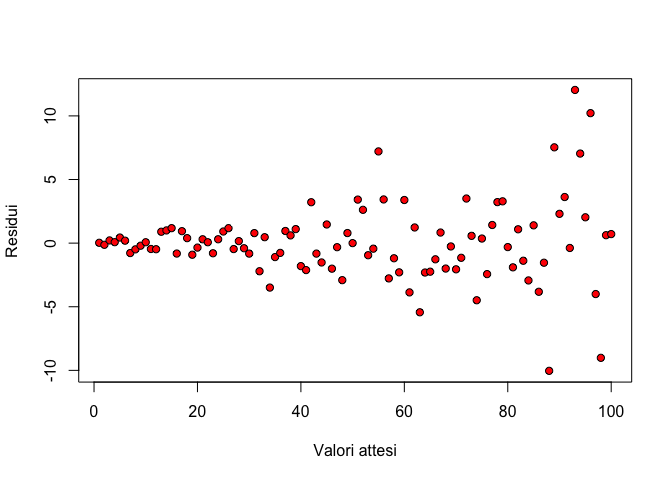
\includegraphics{_main_files/figure-latex/unnamed-chunk-59-1.pdf}

Più formalmente, si può dimostrare che la sampling distribution di F è
data dalla distribuzione F di Fisher, con 4 gradi di libertà al
numeratore e 35 al denominatore (in blue in figura).

Di conseguenza, possiamo utilizzare la F di Fisher per calcolare la
probabilità di ottenere un valore di F altrettanto estremo o più estremo
del nostro. Ad esempio, in R, possiamo utilizzare la funzione:

\begin{Shaded}
\begin{Highlighting}[]
\DecValTok{1} \OperatorTok{-}\StringTok{ }\KeywordTok{pf}\NormalTok{(Foss, }\DecValTok{4}\NormalTok{, }\DecValTok{35}\NormalTok{)}
\NormalTok{## [1] 0}
\end{Highlighting}
\end{Shaded}

praticamente pari a 0. Insomma, in assenza di un effetto del trattamento
(quindi per il solo effetto del caso), se ripetiamo l'esperimento
infinite volte, abbiamo abbiamo una probabilità praticamente nulla che
si produca un valore di F altrettanto alto o più alto di quello da noi
osservato.

Di conseguenza, se rifiutiamo l'ipotesi nulla di assenza di effetto del
trattamento e accettiamo l'ipotesi alternativa (il trattamento ha avuto
effetto significativo) ci portiamo dietro un rischio di errore
estremamente piccolo, comunque molto al disotto della soglia prefissata
del 5\%.

INSOMMA:

\begin{enumerate}
\def\labelenumi{\arabic{enumi}.}
\tightlist
\item
  Con l'ANOVA la variabilità totale dei dati viene decomposta in due
  quote, una attribuibile al trattamento sperimentale ed una
  inspiegabile (residuo)
\item
  L'effetto del trattamento è significativo, se la variabilità che esso
  provoca è superiore a quella inspiegabile
\item
  Confronto tra varianze (test F). L'ipotesi nulla è che il trattamento
  NON E' significativo
\item
  P rappresenta la probabilità di errore nel rifiutare l'ipotesi nulla
\item
  L'ipotesi nulla è rifiutata quando P \(\leq\) 0.05 (livello di
  protezione arbitrario, ma universalmente accettato)
\end{enumerate}

La tabella finale dell'ANOVA può essere ottenuta in R utilizzando la
seguente funzione.

\begin{Shaded}
\begin{Highlighting}[]
\KeywordTok{anova}\NormalTok{(mod)}
\NormalTok{## Analysis of Variance Table}
\NormalTok{## }
\NormalTok{## Response: Y}
\NormalTok{##               Df Sum Sq Mean Sq F value    Pr(>F)    }
\NormalTok{## factor(treat)  4 4013.6 1003.41  505.63 < 2.2e-16 ***}
\NormalTok{## Residuals     35   69.5    1.98                      }
\NormalTok{## ---}
\NormalTok{## Signif. codes:  0 '***' 0.001 '**' 0.01 '*' 0.05 '.' 0.1 ' ' 1}
\end{Highlighting}
\end{Shaded}

Ovviamente, è necessario ricordare che tutte le considerazioni fatte
finora sono valide se il dataset è conforme alle assunzioni di base per
l'anova, cioè normalità dei residui e omogeneità delle varianze. In
questo caso sappiamo che è vero, in generale bisogna eseguire i
necessari controlli, di cui parleremo in un prossimo capitolo.

\section{Per approfondimenti}\label{per-approfondimenti-1}

Kuehl, R. O., 2000. Design of experiments: statistical principles of
research design and analysis. Duxbury Press (CHAPTER 2)

\chapter{La verifica delle assunzioni di base: metodi
diagnostici}\label{la-verifica-delle-assunzioni-di-base-metodi-diagnostici}

\section{Introduzione}\label{introduzione-2}

Nel momento in cui eseguiamo test d'ipotesi nell'ambito di un modello
lineare, assumiamo implicitamente che i dati rispondano ai seguenti
requisiti:

\begin{enumerate}
\def\labelenumi{\arabic{enumi}.}
\tightlist
\item
  il modello è corretto;
\item
  la risposta osservata è una funzione del modello più o meno l'errore
  sperimentale;
\item
  l' errore sperimentale è indipendente dal modello;
\item
  gli errori sono normalmente distribuiti, con media zero e varianze
  omogenee;
\item
  gli errori rilevati in esperimenti ripetuti sono tra loro
  indipendenti.
\item
  assenza di osservazioni aberranti;
\end{enumerate}

In genere, le assunzioni di base non possono essere verificate \emph{a
priori}, perché per quasi nessuno dei fenomeni naturali sono note le
vere relazioni causa-effetto. Per questo motivo, si procede in primo
luogo al fitting del modello e, successivamente, si verifica il rispetto
delle assunzioni di base.

Il problema è importante perché ogni deviazione rispetto agli anzidetti
requisiti può inficiare la validità dei test d'ipotesi, modificando il
livello di significatività. A proposito dei dati aberranti, dobbiamo
dire che, se è sbagliato correggerli arbitrariamente, senza aver prima
accertato che siano effettivamente frutto di errore, potrebbe essere
altrettanto sbagliato lasciarli nel dataset, in quanto essi possono
influenzare in modo molto marcato il risultato dell'analisi. E'evidente
comunque che l'eventuale correzione dovrebbe riguardare una larga
minoranza dei dati sperimentali raccolti (orientativamente, non più del
5\%), altrimenti si dovrà necessariamente pensare di ripetere
l'esperimento.

\section{Procedure diagnostiche}\label{procedure-diagnostiche}

In questo capitolo ci occuperemo di diverse procedure, così
classificate:

\begin{enumerate}
\def\labelenumi{\arabic{enumi}.}
\tightlist
\item
  ispezione grafica dei residui
\item
  test di Anscombe e Tukey per la ricerca degli outliers
\item
  test di Bartlett e test di Levene per l'omogeneità delle varianze
\item
  Procedura di Box e Cox per la scelta delle trasformazioni
  stabilizzanti
\end{enumerate}

\section{Analisi grafica dei residui}\label{analisi-grafica-dei-residui}

La gran parte dei pre-requisiti fondamentali di un dataset riguardano la
struttura dei residui e, di conseguenza, l'ispezione grafica di questi
ultimi, eventualmente accompagnata da semplici strumenti algebrici,
possono permetterci di evidenziare la gran parte delle 'patologie' di
cui soffrono i dati sperimentali. Si può affermare che l'ispezione dei
residui è uno strumento diagnostico fondamentale il cui impiego dovrebbe
rientrare tra le metodiche di routine per ogni elaborazione statistica
dei dati.

Ricordo che i residui sono gli scostamenti tra i valori osservati e
quelli attesi sulla base del modello in studio; hanno sempre media 0,
mentre la deviazione standard cambia di volta in volta.

\subsection{Grafico dei residui contro i valori
attesi}\label{grafico-dei-residui-contro-i-valori-attesi}

Il metodo grafico più utilizzato per l'analisi dei residui consiste nel
plottare i residui verso i valori attesi. Se non vi sono problemi, i
punti nel grafico dovrebbero essere distribuiti in modo assolutamente
casuale, come nel grafico sottostante.

\begin{Shaded}
\begin{Highlighting}[]
\KeywordTok{set.seed}\NormalTok{(}\DecValTok{1234}\NormalTok{)}
\KeywordTok{plot}\NormalTok{(}\KeywordTok{rnorm}\NormalTok{(}\DecValTok{100}\NormalTok{, }\DecValTok{0}\NormalTok{, }\FloatTok{2.5}\NormalTok{) }\OperatorTok{~}\StringTok{ }\KeywordTok{c}\NormalTok{(}\DecValTok{1}\OperatorTok{:}\DecValTok{100}\NormalTok{), }\DataTypeTok{xlab=}\StringTok{"Valori attesi"}\NormalTok{, }
     \DataTypeTok{ylab =} \StringTok{"Residui"}\NormalTok{, }\DataTypeTok{pch=}\DecValTok{21}\NormalTok{, }\DataTypeTok{bg=}\StringTok{"red"}\NormalTok{)}
\end{Highlighting}
\end{Shaded}

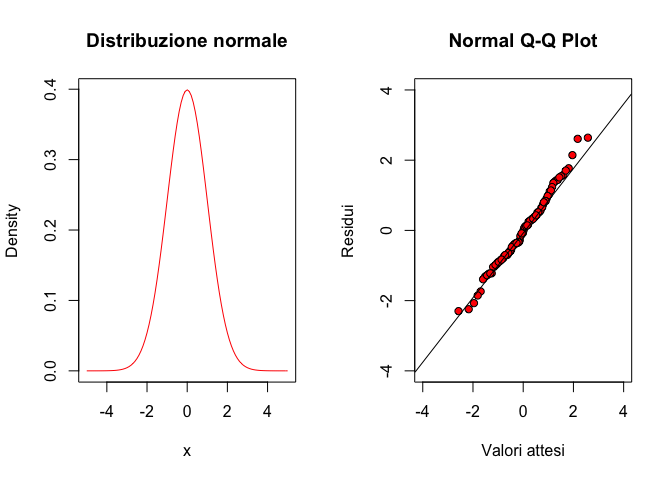
\includegraphics{_main_files/figure-latex/unnamed-chunk-62-1.pdf}

Le osservazioni aberranti (\emph{outliers}) sono chiaramente indicate
nel grafico dei residui come punti isolati rispetto agli altri (Figura
sottostante).

\begin{Shaded}
\begin{Highlighting}[]
\KeywordTok{set.seed}\NormalTok{(}\DecValTok{122}\NormalTok{)}
\KeywordTok{plot}\NormalTok{(}\KeywordTok{c}\NormalTok{(}\KeywordTok{rnorm}\NormalTok{(}\DecValTok{100}\NormalTok{, }\DecValTok{0}\NormalTok{,}\FloatTok{2.5}\NormalTok{), }\DecValTok{16}\NormalTok{) }\OperatorTok{~}\StringTok{ }\KeywordTok{c}\NormalTok{(}\DecValTok{1}\OperatorTok{:}\DecValTok{100}\NormalTok{, }\DecValTok{60}\NormalTok{), }\DataTypeTok{xlab=}\StringTok{"Valori attesi"}\NormalTok{, }
     \DataTypeTok{ylab =} \StringTok{"Residui"}\NormalTok{, }\DataTypeTok{pch=}\DecValTok{21}\NormalTok{, }\DataTypeTok{bg=}\StringTok{"red"}\NormalTok{)}
\end{Highlighting}
\end{Shaded}

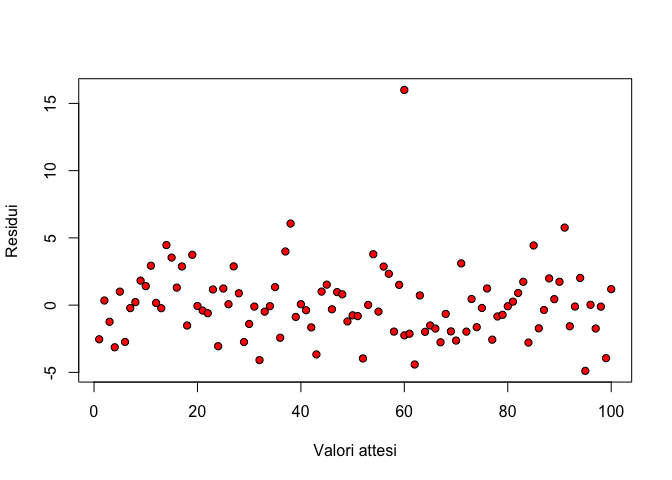
\includegraphics{_main_files/figure-latex/unnamed-chunk-63-1.pdf}

L'eterogeneità delle varianze è invece indicata da residui che si
allargano o si stringono procedendo verso i margini del grafico (Figura
sottostante), facendo emergere una sorta di proporzionalità tra media e
varianza.

\begin{Shaded}
\begin{Highlighting}[]
\KeywordTok{set.seed}\NormalTok{(}\DecValTok{424}\NormalTok{)}
\NormalTok{dati <-}\StringTok{ }\KeywordTok{c}\NormalTok{(}\DecValTok{1}\OperatorTok{:}\DecValTok{100}\NormalTok{)}
\KeywordTok{plot}\NormalTok{(}\KeywordTok{rnorm}\NormalTok{(}\DecValTok{100}\NormalTok{, }\DecValTok{0}\NormalTok{, dati}\OperatorTok{/}\DecValTok{20}\NormalTok{) }\OperatorTok{~}\StringTok{ }\NormalTok{dati, }\DataTypeTok{xlab=}\StringTok{"Valori attesi"}\NormalTok{, }
     \DataTypeTok{ylab =} \StringTok{"Residui"}\NormalTok{, }\DataTypeTok{pch=}\DecValTok{21}\NormalTok{, }\DataTypeTok{bg=}\StringTok{"red"}\NormalTok{)}
\end{Highlighting}
\end{Shaded}

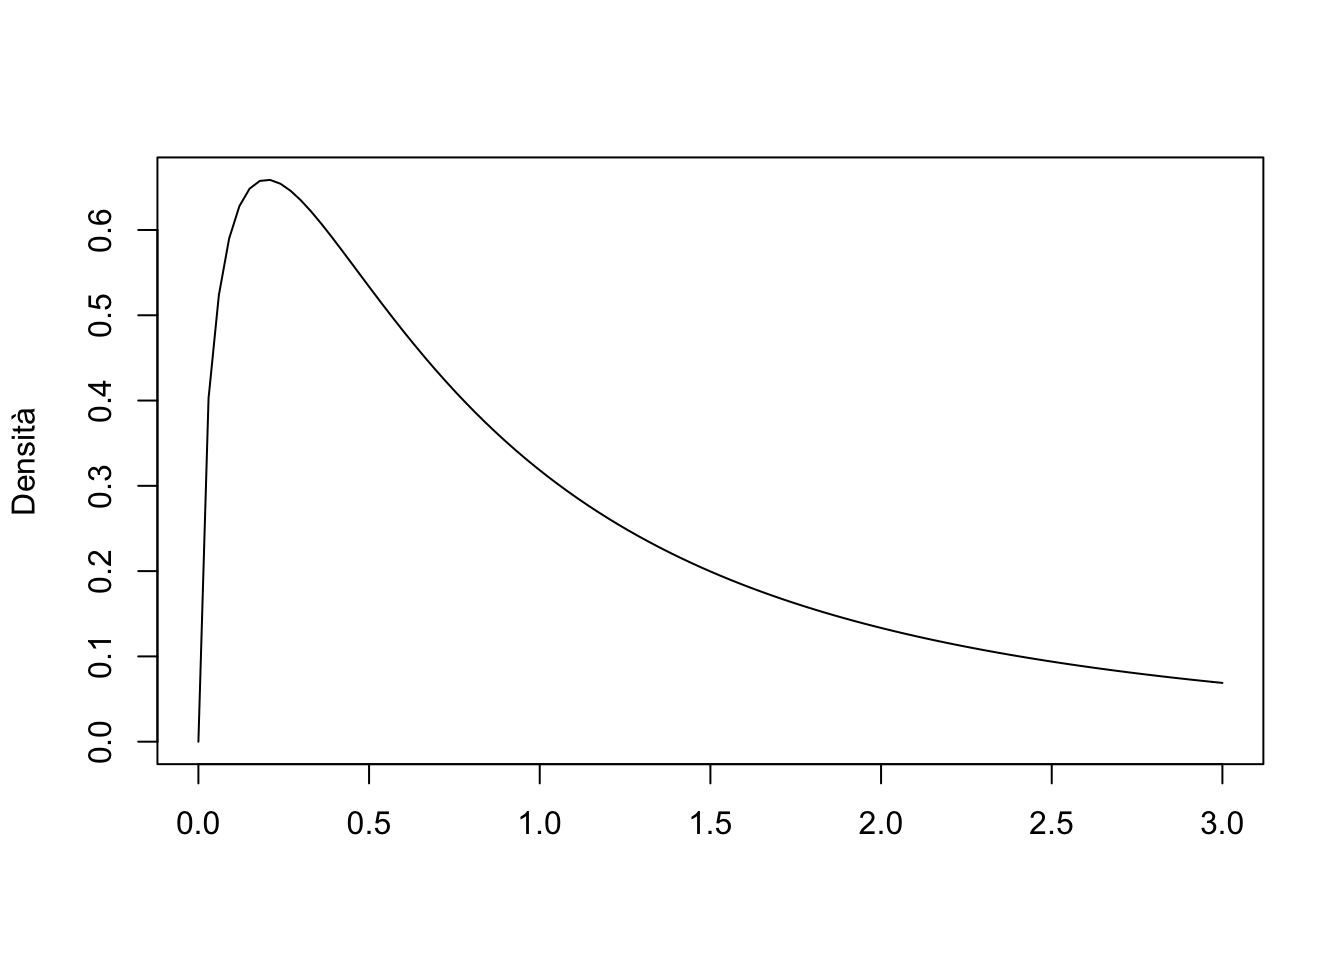
\includegraphics{_main_files/figure-latex/unnamed-chunk-64-1.pdf}

A volte la relazione causa effetto non è lineare o, comunque, il modello
devia sistematicamente dai dati osservati. Di conseguenza, i residui
mostrano un evidente pattern legato al segno. Ad esempio, i residui sono
tendenzialmente negativi per bassi valori attesi e positivi per alti
valori.

\begin{Shaded}
\begin{Highlighting}[]
\KeywordTok{set.seed}\NormalTok{(}\DecValTok{424}\NormalTok{)}
\NormalTok{dati <-}\StringTok{ }\KeywordTok{c}\NormalTok{(}\DecValTok{1}\OperatorTok{:}\DecValTok{100}\NormalTok{)}
\KeywordTok{plot}\NormalTok{(}\KeywordTok{rnorm}\NormalTok{(}\DecValTok{100}\NormalTok{, }\OperatorTok{-}\DecValTok{5} \OperatorTok{+}\StringTok{ }\FloatTok{0.1}\OperatorTok{*}\NormalTok{dati, }\FloatTok{1.5}\NormalTok{) }\OperatorTok{~}\StringTok{ }\NormalTok{dati, }\DataTypeTok{xlab=}\StringTok{"Valori attesi"}\NormalTok{, }\DataTypeTok{ylab =} \StringTok{"Residui"}\NormalTok{, }\DataTypeTok{pch=}\DecValTok{21}\NormalTok{, }\DataTypeTok{bg=}\StringTok{"red"}\NormalTok{)}
\KeywordTok{abline}\NormalTok{()}
\end{Highlighting}
\end{Shaded}

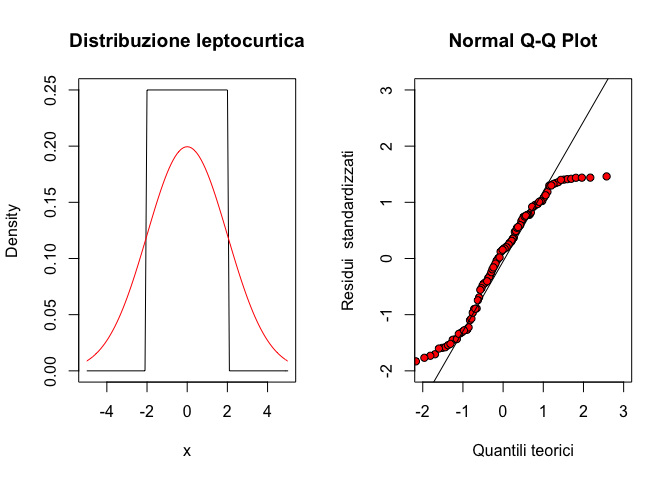
\includegraphics{_main_files/figure-latex/unnamed-chunk-65-1.pdf}

\subsection{QQ-plot}\label{qq-plot}

Il grafico dei residui verso i valori attesi non è invece in grado di
evidenza problemi di non-normalità. A questo fine, risulta molto utile
un QQ-plot (quantile-quantile plot), nel quale i residui
\emph{standardizzati} vengono plottati contro i rispettivi quantili di
una distribuzione normale standardizzata (figura sottostante).

\begin{Shaded}
\begin{Highlighting}[]
\KeywordTok{par}\NormalTok{(}\DataTypeTok{mfrow=}\KeywordTok{c}\NormalTok{(}\DecValTok{1}\NormalTok{,}\DecValTok{2}\NormalTok{))}
\KeywordTok{curve}\NormalTok{(}\KeywordTok{dnorm}\NormalTok{(x, }\DecValTok{0}\NormalTok{, }\DecValTok{1}\NormalTok{), }\DataTypeTok{from=}\OperatorTok{-}\DecValTok{5}\NormalTok{, }\DataTypeTok{to=}\DecValTok{5}\NormalTok{, }\DataTypeTok{col=}\StringTok{"red"}\NormalTok{,}
      \DataTypeTok{ylab=}\StringTok{"Density"}\NormalTok{, }\DataTypeTok{main=}\StringTok{"Distribuzione normale"}\NormalTok{)}
\KeywordTok{set.seed}\NormalTok{(}\DecValTok{424}\NormalTok{)}
\NormalTok{res <-}\StringTok{ }\KeywordTok{scale}\NormalTok{(}\KeywordTok{rnorm}\NormalTok{(}\DecValTok{100}\NormalTok{, }\DecValTok{0}\NormalTok{, }\FloatTok{2.5}\NormalTok{), }\DataTypeTok{scale=}\NormalTok{T)}
\KeywordTok{qqnorm}\NormalTok{(res, }\DataTypeTok{xlab=}\StringTok{"Valori attesi"}\NormalTok{, }
     \DataTypeTok{ylab =} \StringTok{"Residui"}\NormalTok{, }\DataTypeTok{pch=}\DecValTok{21}\NormalTok{, }\DataTypeTok{bg=}\StringTok{"red"}\NormalTok{, }\DataTypeTok{xlim=}\KeywordTok{c}\NormalTok{(}\OperatorTok{-}\DecValTok{4}\NormalTok{,}\DecValTok{4}\NormalTok{),}
     \DataTypeTok{ylim=}\KeywordTok{c}\NormalTok{(}\OperatorTok{-}\DecValTok{4}\NormalTok{,}\DecValTok{4}\NormalTok{))}
\KeywordTok{qqline}\NormalTok{(res)}
\end{Highlighting}
\end{Shaded}

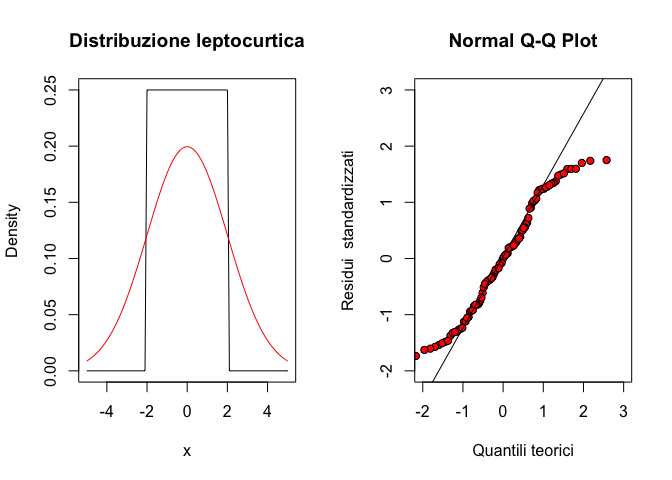
\includegraphics{_main_files/figure-latex/unnamed-chunk-66-1.pdf}

Le deviazioni più diffuse dalla normalità sono relative alla simmetria
(skewness) e alla curtosi della popolazione. In particolare, i nostri
residui potrebbero avere asimmetria positiva (right-skewed: la media è
maggiore della mediana), in modo che abbiamo più residui negativi che
positivi, mentre questi ultimi sono mediamente di più elevato valore
assoluto. Ad esempio, una distribuzione log-normale centrata è
right-skewed. In questa situazione, i residui alti positivi dovrebbero
avere una maggior frequenza che nella distribuzione normale
corrispondente, al contrario di quelli bassi negativi.

\begin{Shaded}
\begin{Highlighting}[]
\KeywordTok{par}\NormalTok{(}\DataTypeTok{mfrow=}\KeywordTok{c}\NormalTok{(}\DecValTok{1}\NormalTok{,}\DecValTok{2}\NormalTok{))}
\KeywordTok{curve}\NormalTok{(}\KeywordTok{dnorm}\NormalTok{(x, }\DecValTok{0}\NormalTok{, }\DecValTok{1}\NormalTok{), }\DataTypeTok{from=}\OperatorTok{-}\DecValTok{5}\NormalTok{, }\DataTypeTok{to=}\DecValTok{5}\NormalTok{, }\DataTypeTok{col=}\StringTok{"red"}\NormalTok{,}
      \DataTypeTok{ylab=}\StringTok{"Density"}\NormalTok{, }\DataTypeTok{main=}\StringTok{"Asimmetria positiva"}\NormalTok{,}
      \DataTypeTok{ylim=}\KeywordTok{c}\NormalTok{(}\DecValTok{0}\NormalTok{,}\FloatTok{0.5}\NormalTok{))}
\KeywordTok{curve}\NormalTok{(}\KeywordTok{dlnorm}\NormalTok{(x }\OperatorTok{+}\StringTok{ }\DecValTok{3}\NormalTok{, }\KeywordTok{log}\NormalTok{(}\DecValTok{3}\NormalTok{), }\FloatTok{0.35}\NormalTok{), }\DataTypeTok{add=}\NormalTok{T)}
\KeywordTok{legend}\NormalTok{(}\StringTok{"topright"}\NormalTok{, }\DataTypeTok{legend=}\KeywordTok{c}\NormalTok{(}\StringTok{"n"}\NormalTok{, }\StringTok{"log-n"}\NormalTok{),}
       \DataTypeTok{lty=}\KeywordTok{c}\NormalTok{(}\DecValTok{1}\NormalTok{,}\DecValTok{1}\NormalTok{), }\DataTypeTok{col=}\KeywordTok{c}\NormalTok{(}\StringTok{"red"}\NormalTok{, }\StringTok{"black"}\NormalTok{), }\DataTypeTok{bty=}\StringTok{"n"}\NormalTok{)}

\CommentTok{#Estraggo una campione da una log-normale}
\KeywordTok{set.seed}\NormalTok{(}\DecValTok{1234}\NormalTok{)}
\NormalTok{d <-}\StringTok{ }\KeywordTok{rlnorm}\NormalTok{(}\DecValTok{100}\NormalTok{, }\DecValTok{2}\NormalTok{, }\FloatTok{0.5}\NormalTok{)}
\NormalTok{res <-}\StringTok{ }\KeywordTok{scale}\NormalTok{(d, }\DataTypeTok{scale=}\NormalTok{T)}

\CommentTok{#Produco un QQ-plot}
\KeywordTok{qqnorm}\NormalTok{(res, }\DataTypeTok{xlab=}\StringTok{"Quantili teorici"}\NormalTok{, }
     \DataTypeTok{ylab =} \StringTok{"Residui  standardizzati"}\NormalTok{, }
     \DataTypeTok{pch=}\DecValTok{21}\NormalTok{, }\DataTypeTok{bg=}\StringTok{"red"}\NormalTok{, }\DataTypeTok{xlim=}\KeywordTok{c}\NormalTok{(}\OperatorTok{-}\DecValTok{4}\NormalTok{,}\DecValTok{4}\NormalTok{), }\DataTypeTok{ylim=}\KeywordTok{c}\NormalTok{(}\OperatorTok{-}\DecValTok{4}\NormalTok{,}\DecValTok{4}\NormalTok{))}
\KeywordTok{qqline}\NormalTok{(res)}
\end{Highlighting}
\end{Shaded}

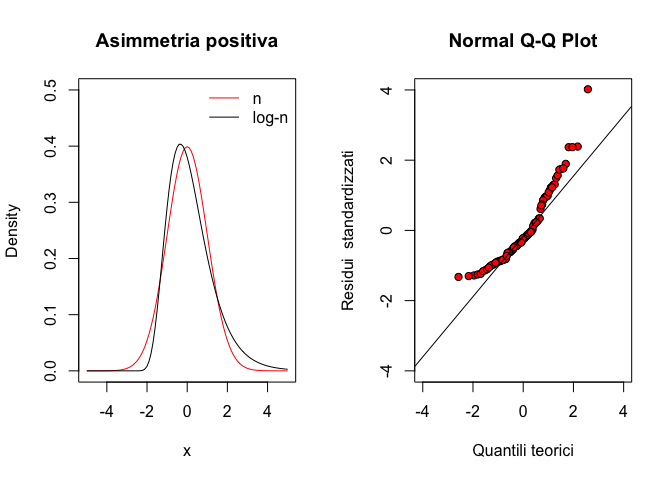
\includegraphics{_main_files/figure-latex/unnamed-chunk-67-1.pdf}

Al contrario, una distribuzione left-skewed (skewness negativo, cioè
media minore della mediana; esempio: una distribuzione beta con
traslazione, alto \(a\) e basso \(b\)), si comporta come indicato nel
grafico seguente:

\begin{Shaded}
\begin{Highlighting}[]
\CommentTok{#Estraggo una campione da una distribuzione beta}
\KeywordTok{par}\NormalTok{(}\DataTypeTok{mfrow=}\KeywordTok{c}\NormalTok{(}\DecValTok{1}\NormalTok{,}\DecValTok{2}\NormalTok{))}
\KeywordTok{curve}\NormalTok{(}\KeywordTok{dnorm}\NormalTok{(x, }\DecValTok{0}\NormalTok{, }\FloatTok{0.10}\NormalTok{), }\DataTypeTok{from=}\OperatorTok{-}\FloatTok{0.6}\NormalTok{, }\DataTypeTok{to=}\FloatTok{0.6}\NormalTok{, }\DataTypeTok{col=}\StringTok{"red"}\NormalTok{, }
      \DataTypeTok{ylab=}\StringTok{"Density"}\NormalTok{, }\DataTypeTok{main=}\StringTok{"Asimmetria negativa"}\NormalTok{,}
      \DataTypeTok{ylim=}\KeywordTok{c}\NormalTok{(}\DecValTok{0}\NormalTok{,}\DecValTok{5}\NormalTok{))}
\KeywordTok{curve}\NormalTok{(}\KeywordTok{dbeta}\NormalTok{(x }\OperatorTok{+}\StringTok{ }\FloatTok{0.8}\NormalTok{, }\DecValTok{8}\NormalTok{, }\DecValTok{2}\NormalTok{), }\DataTypeTok{add=}\NormalTok{T)}
\KeywordTok{legend}\NormalTok{(}\StringTok{"topleft"}\NormalTok{, }\DataTypeTok{legend=}\KeywordTok{c}\NormalTok{(}\StringTok{"normale"}\NormalTok{, }\StringTok{"beta"}\NormalTok{),}
       \DataTypeTok{lty=}\KeywordTok{c}\NormalTok{(}\DecValTok{1}\NormalTok{,}\DecValTok{1}\NormalTok{), }\DataTypeTok{col=}\KeywordTok{c}\NormalTok{(}\StringTok{"red"}\NormalTok{, }\StringTok{"black"}\NormalTok{), }\DataTypeTok{bty=}\StringTok{"n"}\NormalTok{)}
\KeywordTok{set.seed}\NormalTok{(}\DecValTok{1230}\NormalTok{)}
\NormalTok{d <-}\StringTok{ }\KeywordTok{rbeta}\NormalTok{(}\DecValTok{100}\NormalTok{, }\DecValTok{8}\NormalTok{, }\DecValTok{2}\NormalTok{)}
\NormalTok{res <-}\StringTok{ }\KeywordTok{scale}\NormalTok{(d, }\DataTypeTok{scale=}\NormalTok{T)}
\CommentTok{#Produco un QQ-plot}
\KeywordTok{qqnorm}\NormalTok{(res, }\DataTypeTok{xlab=}\StringTok{"Quantili teorici"}\NormalTok{, }
     \DataTypeTok{ylab =} \StringTok{"Residui  standardizzati"}\NormalTok{, }
     \DataTypeTok{pch=}\DecValTok{21}\NormalTok{, }\DataTypeTok{bg=}\StringTok{"red"}\NormalTok{, }\DataTypeTok{xlim=}\KeywordTok{c}\NormalTok{(}\OperatorTok{-}\DecValTok{2}\NormalTok{,}\DecValTok{3}\NormalTok{), }\DataTypeTok{ylim=}\KeywordTok{c}\NormalTok{(}\OperatorTok{-}\DecValTok{2}\NormalTok{,}\DecValTok{3}\NormalTok{))}
\KeywordTok{qqline}\NormalTok{(res)}
\end{Highlighting}
\end{Shaded}

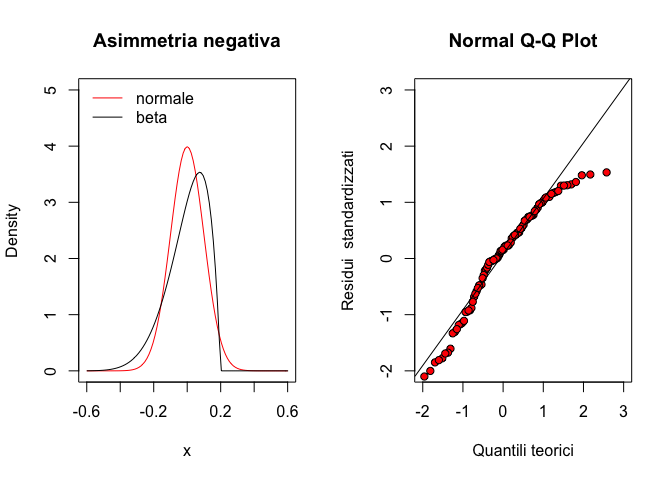
\includegraphics{_main_files/figure-latex/unnamed-chunk-68-1.pdf}

Per quanto riguarda la curtosi, è necessario osservare le code della
distribuzione: se queste sono più alte di una distribuzione normale
parliamo di distribuzione platicurtica, come, ad esempio, una
distribuzione di t di Student con pochi gradi di libertà.

\begin{Shaded}
\begin{Highlighting}[]
\CommentTok{#Estraggo una campione da una t di Student}
\KeywordTok{par}\NormalTok{(}\DataTypeTok{mfrow=}\KeywordTok{c}\NormalTok{(}\DecValTok{1}\NormalTok{,}\DecValTok{2}\NormalTok{))}
\KeywordTok{curve}\NormalTok{(}\KeywordTok{dnorm}\NormalTok{(x), }\DataTypeTok{from=}\OperatorTok{-}\DecValTok{5}\NormalTok{, }\DataTypeTok{to=}\DecValTok{5}\NormalTok{, }\DataTypeTok{col=}\StringTok{"red"}\NormalTok{, }
      \DataTypeTok{ylab=}\StringTok{"Density"}\NormalTok{, }\DataTypeTok{main=}\StringTok{"Distribuzione platicurtica"}\NormalTok{)}
\KeywordTok{curve}\NormalTok{(}\KeywordTok{dt}\NormalTok{(x, }\DecValTok{1}\NormalTok{), }\DataTypeTok{add=}\NormalTok{T)}
\KeywordTok{legend}\NormalTok{(}\StringTok{"topleft"}\NormalTok{, }\DataTypeTok{legend=}\KeywordTok{c}\NormalTok{(}\StringTok{"normale"}\NormalTok{, }\StringTok{"t (1 DF)"}\NormalTok{),}
       \DataTypeTok{lty=}\KeywordTok{c}\NormalTok{(}\DecValTok{1}\NormalTok{,}\DecValTok{1}\NormalTok{), }\DataTypeTok{col=}\KeywordTok{c}\NormalTok{(}\StringTok{"red"}\NormalTok{, }\StringTok{"black"}\NormalTok{), }\DataTypeTok{bty=}\StringTok{"n"}\NormalTok{)}
\KeywordTok{set.seed}\NormalTok{(}\DecValTok{1230}\NormalTok{)}
\NormalTok{d <-}\StringTok{ }\KeywordTok{rt}\NormalTok{(}\DecValTok{100}\NormalTok{, }\DecValTok{1}\NormalTok{)}
\NormalTok{res <-}\StringTok{ }\KeywordTok{scale}\NormalTok{(d, }\DataTypeTok{scale=}\NormalTok{T)}
\CommentTok{#Produco un QQ-plot}
\KeywordTok{qqnorm}\NormalTok{(res, }\DataTypeTok{xlab=}\StringTok{"Quantili teorici"}\NormalTok{, }
     \DataTypeTok{ylab =} \StringTok{"Residui  standardizzati"}\NormalTok{,}
     \DataTypeTok{pch=}\DecValTok{21}\NormalTok{, }\DataTypeTok{bg=}\StringTok{"red"}\NormalTok{, }\DataTypeTok{xlim=}\KeywordTok{c}\NormalTok{(}\OperatorTok{-}\DecValTok{2}\NormalTok{,}\DecValTok{3}\NormalTok{), }\DataTypeTok{ylim=}\KeywordTok{c}\NormalTok{(}\OperatorTok{-}\DecValTok{2}\NormalTok{,}\DecValTok{3}\NormalTok{))}
\KeywordTok{qqline}\NormalTok{(res)}
\end{Highlighting}
\end{Shaded}

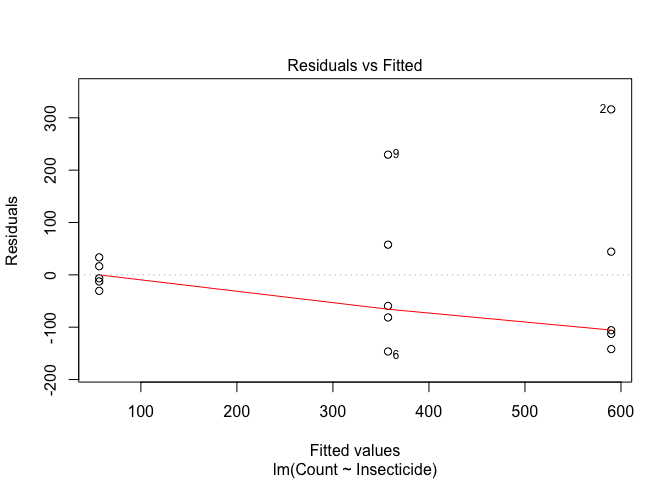
\includegraphics{_main_files/figure-latex/unnamed-chunk-69-1.pdf}

Analogamente, vediamo come si presenta un QQ-plot per una distribuzione
leptocurtica (più bassa sulle code; esempio: distribuzione uniforme).

\begin{Shaded}
\begin{Highlighting}[]
\CommentTok{#Estraggo una campione da una distribuzione uniforme}
\KeywordTok{par}\NormalTok{(}\DataTypeTok{mfrow=}\KeywordTok{c}\NormalTok{(}\DecValTok{1}\NormalTok{,}\DecValTok{2}\NormalTok{))}
\KeywordTok{curve}\NormalTok{(}\KeywordTok{dunif}\NormalTok{(x, }\OperatorTok{-}\DecValTok{2}\NormalTok{,}\DecValTok{2}\NormalTok{), }\DataTypeTok{from=}\OperatorTok{-}\DecValTok{5}\NormalTok{, }\DataTypeTok{to=}\DecValTok{5}\NormalTok{, }\DataTypeTok{ylab=}\StringTok{"Density"}\NormalTok{, }\DataTypeTok{main=}\StringTok{"Distribuzione leptocurtica"}\NormalTok{)}
\KeywordTok{curve}\NormalTok{(}\KeywordTok{dnorm}\NormalTok{(x, }\DecValTok{0}\NormalTok{, }\DecValTok{2}\NormalTok{), }\DataTypeTok{add=}\NormalTok{T, }\DataTypeTok{col=}\StringTok{"red"}\NormalTok{)}
\KeywordTok{set.seed}\NormalTok{(}\DecValTok{1230}\NormalTok{)}
\NormalTok{d <-}\StringTok{ }\KeywordTok{runif}\NormalTok{(}\DecValTok{100}\NormalTok{, }\OperatorTok{-}\DecValTok{2}\NormalTok{, }\DecValTok{2}\NormalTok{)}
\NormalTok{res <-}\StringTok{ }\KeywordTok{scale}\NormalTok{(d, }\DataTypeTok{scale=}\NormalTok{T)}
\CommentTok{#Produco un QQ-plot}
\KeywordTok{qqnorm}\NormalTok{(res, }\DataTypeTok{xlab=}\StringTok{"Quantili teorici"}\NormalTok{, }
     \DataTypeTok{ylab =} \StringTok{"Residui  standardizzati"}\NormalTok{, }
     \DataTypeTok{pch=}\DecValTok{21}\NormalTok{, }\DataTypeTok{bg=}\StringTok{"red"}\NormalTok{, }\DataTypeTok{xlim=}\KeywordTok{c}\NormalTok{(}\OperatorTok{-}\DecValTok{2}\NormalTok{,}\DecValTok{3}\NormalTok{), }\DataTypeTok{ylim=}\KeywordTok{c}\NormalTok{(}\OperatorTok{-}\DecValTok{2}\NormalTok{,}\DecValTok{3}\NormalTok{))}
\KeywordTok{qqline}\NormalTok{(res)}
\end{Highlighting}
\end{Shaded}

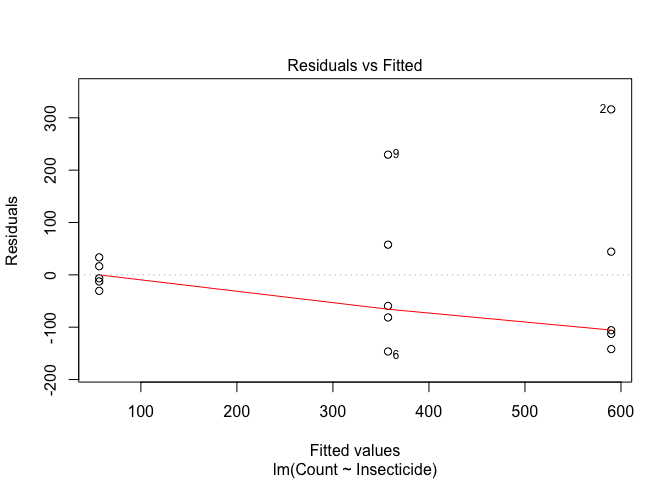
\includegraphics{_main_files/figure-latex/unnamed-chunk-70-1.pdf}

\section{Altri strumenti diagnostici}\label{altri-strumenti-diagnostici}

La valutazioni precedentemente esposte sono di tipo grafico e sono
considerate sufficientemente robuste per la maggior parte delle
situazioni. Tuttavia, esistono anche test statistici che consentono di
saggiare l'ipotesi nulla di 'assenza di deviazioni'. Per tutti questi
test, l'ipotesi nulla è quella di assenza di deviazioni. Pertanto, basta
guardare il 'p value': se questo è inferiore a 0.05 l'ipotesi nulla deve
essere rifiutata e può essere necessario intraprendere azioni
correttive.

Per l'omogeneità delle varianze veniva utilizzato il test di Bartlett,
che, tuttavia, è oggi caduto in disuso, data la sua sensibilità alla
non-normalità dei residui, quasi sempre presente, insieme
all'eteroscedasticità. Oggi si preferisce utilizzare il test di Levene,
che consiste in un'ANOVA dei residui, al posto dei dati osservati:

\begin{Shaded}
\begin{Highlighting}[]
\KeywordTok{library}\NormalTok{(aomisc)}
\KeywordTok{data}\NormalTok{(sinapis)}
\KeywordTok{head}\NormalTok{(sinapis)}
\NormalTok{##   density yield}
\NormalTok{## 1       0 36.63}
\NormalTok{## 2      14 29.73}
\NormalTok{## 3      19 32.12}
\NormalTok{## 4      28 30.61}
\NormalTok{## 5      32 27.70}
\NormalTok{## 6      38 27.43}
\NormalTok{model <-}\StringTok{ }\KeywordTok{lm}\NormalTok{(yield }\OperatorTok{~}\StringTok{ }\KeywordTok{factor}\NormalTok{(density), }\DataTypeTok{data=}\NormalTok{sinapis)}
\KeywordTok{anova}\NormalTok{( }\KeywordTok{lm}\NormalTok{ (}\KeywordTok{abs}\NormalTok{(}\KeywordTok{residuals}\NormalTok{(model)) }\OperatorTok{~}\StringTok{ }\KeywordTok{factor}\NormalTok{(density), }\DataTypeTok{data=}\NormalTok{sinapis))}
\NormalTok{## Analysis of Variance Table}
\NormalTok{## }
\NormalTok{## Response: abs(residuals(model))}
\NormalTok{##                 Df  Sum Sq Mean Sq F value Pr(>F)}
\NormalTok{## factor(density)  6  8.4359 1.40598  1.4215 0.2531}
\NormalTok{## Residuals       21 20.7714 0.98911}
\NormalTok{car}\OperatorTok{::}\KeywordTok{leveneTest}\NormalTok{(yield }\OperatorTok{~}\StringTok{ }\KeywordTok{factor}\NormalTok{(density), }\DataTypeTok{data=}\NormalTok{sinapis, }\DataTypeTok{center=}\NormalTok{mean)}
\NormalTok{## Levene's Test for Homogeneity of Variance (center = mean)}
\NormalTok{##       Df F value Pr(>F)}
\NormalTok{## group  6  1.4215 0.2531}
\NormalTok{##       21}
\end{Highlighting}
\end{Shaded}

Il test di Levene può anche essere effettuato considerando gli scarti
rispetto alla mediana (invece che alla media), in modo da ottenere un
test più robusto nei confronti degli outliers.

Per quanto riguarda le deviazioni dalla normalità, può essere utilizzato
il test di Shapiro-Wilks. Per esempio, nel caso di un dataset ottenuto
da una distribuzione uniforme, il test di Shapiro porta ai risultati
sotto indicati.

\begin{Shaded}
\begin{Highlighting}[]
\KeywordTok{shapiro.test}\NormalTok{(}\KeywordTok{runif}\NormalTok{(}\DecValTok{100}\NormalTok{, }\DataTypeTok{min =} \OperatorTok{-}\DecValTok{2}\NormalTok{, }\DataTypeTok{max =} \DecValTok{2}\NormalTok{))}
\NormalTok{## }
\NormalTok{##  Shapiro-Wilk normality test}
\NormalTok{## }
\NormalTok{## data:  runif(100, min = -2, max = 2)}
\NormalTok{## W = 0.94318, p-value = 0.0003028}
\end{Highlighting}
\end{Shaded}

\section{Risultati contraddittori}\label{risultati-contraddittori}

La valutazione degli assunti di base è un passo fondamentale
nell'analisi dei dati sperimentali è non può essere evitata in nessun
modo. Il problema è importante perché ogni deviazione rispetto agli
anzidetti requisiti può inficiare la validità dei test d'ipotesi,
modificando il livello di significatività e di protezione.

Tuttavia, ricordiamo sempre che la 'verità vera' ci sfugge e, di
conseguenza, le valutazioni sull'adozione di eventuali trasformazioni
stabilizzanti debbono essere condotte con il massimo 'buon senso'!

In particolare nella pratica è molto facile incontrare situazioni
dubbie, nelle quali l'analisi dei residui mostra deviazioni, mentre il
test di Bartlett è significativo e quello di Levene no. Come
comportarsi? Misurare sempre la forza dell'evidenza 'patologica': quanti
campanelli di allarme abbiamo?

\section{\texorpdfstring{`Terapia'}{Terapia}}\label{terapia}

Se le procedure diagnostiche hanno evidenziato deviazioni rispetto agli
assunti di base, è necessario valutare se e come intraprendere azioni
correttive. Ovviamente, la `terapia' cambia al cambiare della
`patologia'.

\subsection{Correzione/Rimozione degli
outliers}\label{correzionerimozione-degli-outliers}

In presenza di outliers, la `terapia' più opportuna è, banalmente,
quella di rimuoverli, ottenendo così un dataset `sbilanciato' (diverso
numero di repliche per trattamento). Oggigiorno, trattare un dataset
sbilanciato non costituisce un problema, ovviamente se si utilizzano le
metodiche di analisi opportune. Qualche anno fa, al contrario, si
cercava di evitare lo sbilanciamento a tutti i costi, utilizzando
tecniche di imputing per l'immissione di valori 'ragionevoli' in
sostituzione di quelli mancanti/aberranti.

Ad esempio, se il disegno sperimentale era a randomizzazione completa,
il dato mancante veniva sostituito con la media delle altre repliche. Se
invece il disegno era a blocchi randomizzati, allora si teneva conto non
solo della media del trattamento di cui il dato mancante faceva parte,
ma anche delle media del blocco nel quale esso si trovava. La formula
era la seguente:

\[Y = \frac{tT + rR - G}{(t - 1)(r - 1)}\]

dove \emph{t} è il numero delle tesi, \emph{r} è il numero delle
repliche, \emph{T} è la somma dei dati relativi alla tesi che contiene
il dato mancante (ovviamente escluso quest'ultimo), \emph{R} è la somma
dei dati relativi al blocco che contiene il dato mancante (sempre
escluso quest'ultimo), \emph{G} è il totale generale (escluso il dato
mancante).

Un aspetto da non trascurare è che, imputando un dato, si rimuove lo
sbilanciamento, ma non si recuperano le informazioni mancanti. Infatti
il dato imputato non fornisce informazioni aggiuntive, perché è ottenuti
come combinazione lineare degli altri. Di conseguenza, per ogni dato
imputato, è necessario ridurre di un'unità il numero dei gradi di
libertà della varianza residua, e ricalcolare F, SEM e SED di
conseguenza.

Possiamo comunque ritenere che, oggigiorno, le tecniche di imputing dei
dati aberranti/mancanti sono da ritenersi obsolete. Inoltre, vogliamo
porre l'attenzione sul fatto che i dati aberranti sono dati molto
`influenziali', nel senso che possono influenzare in modo molto marcato
il risultato dell'analisi. Pertanto, se è sbagliato correggerli
arbitrariamente, senza aver prima accertato che siano effettivamente
frutto di errore, è altrettanto sbagliato lasciarli nel dataset.
Ovviamente, la correzione non può che riguardare una larga minoranza dei
dati sperimentali raccolti (uno o due dati), altrimenti si dovrà
necessariamente pensare di ripetere l'esperimento.

\subsection{Correzione del modello}\label{correzione-del-modello}

Abbiamo visto che il modello impiegato potrebbe non essere adatto a
descrivere il dataset (mancanza di adattamento). Gli effetti potrebbero
non essere addittivi, ma moltiplicativi, oppure potrebbero essere
non-lineari. Potrebbero essere presenti asintoti che il nostro modello
non è in grado di descrivere, oppure la crescita/decrescita osservata
potrebbero essere più lente/veloci di quanto la nostra funzione sia in
grado di modellizzare.

Per tutti questi casi, l'unica operazione consigliabile è quella di
modificare il modello, adottando ai dati un diverso modello. Un'altra
strategia è quella di trasformare la variabile dipendente, in modo che
il modello impiegato possa descriverla più correttamente. Ad esempio, se
i dati mostrano un andamento esponenziale, trasformandoli in logaritmo
questi potreanno essere descritti molto meglio con un equazione lineare.

\subsection{Non-normalità dei residui ed eterogeneità delle
varianze}\label{non-normalita-dei-residui-ed-eterogeneita-delle-varianze}

Trattiamo queste due deviazioni insieme in quanto esse sono spesso
associate nello stesso dataset. Entrambe hanno conseguenze gravi: gli
intervalli di confidenza non hanno un buon grado di copertura e i test
d'ipotesi sono invalidi. I reviewer delle riviste scientifiche sono
sempre molto sospettosi delle eventuali deviazioni rispetto agli assunti
di base, soprattutto quando i dati sono non-continui (conteggi e/o
proporzioni) e, di conseguenza, non sono naturalmente riconducibilli ad
una distribuzione normale.

Evidentemente, la cosa più corretta è quella di chiedersi perché il
dataset è non-normale e/o eteroscedastico ed incorporare queste
informazioni nel modello. Ad esempio, un conteggio potrebbe seguire la
distribuzione di Poisson, oppure una serie di proporzioni potrebbero
seguire la distribuzione binomiale. In questi casi potrebbe essere
opportuno utilizzare modelli lineari generalizzati (GLiM), oppure, in
caso di eterogeneità delle varianze, si potrebbero incorporare nel
modello eventuali relazioni di proporzionalità tra media e varianza, con
tecniche di minimi quadrati generalizzati (GLS). Si tratta di tecniche
statistiche piuttosto avanzate, che richiedono una buona esperienza per
essere utilizzate con profitto.

In altri casi si può ricorrere a metodiche statistiche che fanno meno
assunzioni e che, pertanto, sono dette metodiche `non-parametriche'. Di
queste non parleremo, per una questione di preferenze personali: a mio
modo di vedere, utilizzare metodiche non-parametriche è come rinuciare
in partenza a comprendere le basi biologiche del fenomeno e le
intrinseche relazioni causa-effetto che sussistono nella realtà.

Una strategia empirica, ma molto seguita in pratica e caratterizzata da
un'efficacia non disprezzabile, è quella di ricorrere alle
trasformazioni correttive. Con questa tecnica, si va a cercare una
metrica sulla quale le assunzioni di base dell'ANOVA siano rispettate e
si esegue l'elaborazione dei dati trasformati invece che di quelli non
trasformati.

Per i conteggi e per l'eterogeneità delle varianze di variabili
continue, si consiglia la trasformazione in radice quadrata o in
logaritmo, scegliendo in base a quella che consente la miglior
distribuzione dei residui. Per le proporzioni, taluni consigliano la
trasformazione nell'arcoseno della radice del valore, che è implementata
nel package `aomisc', nella funzione `angularTransform()'. Questa
funzione rivceve come input un valore percentuale e resituisce
l'arcoseno della radice quadrata della proporzione corrispondente.

\begin{Shaded}
\begin{Highlighting}[]
\NormalTok{aomisc}\OperatorTok{::}\KeywordTok{angularTransform}\NormalTok{(}\KeywordTok{c}\NormalTok{(}\DecValTok{26}\NormalTok{, }\DecValTok{47}\NormalTok{, }\DecValTok{25}\NormalTok{, }\DecValTok{28}\NormalTok{, }\DecValTok{24}\NormalTok{))}
\NormalTok{## [1] 30.65730 43.28009 30.00000 31.94806 29.33387}
\end{Highlighting}
\end{Shaded}

\subsection{La procedura di Box e Cox}\label{la-procedura-di-box-e-cox}

Per evitare una trasformazione al buio, si può impiegare la procedura
suggerita da Box e Cox (1964), basata su `famiglie di trasformazioni',
tra cui la più diffusa è:

\[ W = \left\{ \begin{array}{ll}
\frac{Y^\lambda}{\lambda - 1} & \quad \textrm{if} \, \lambda \neq 0 \\
\log(Y) & \quad \textrm{if} \, \lambda = 0
\end{array} \right. \]

dove W è la variabile trasformata, Y è la variabile originale e
\(\lambda\) è il parametro che definisce la trasformazione. In
particolare, osserviamo che se \(\lambda\) è pari ad 1 i dati non sono,
di fatto, trasformati, se è pari a 0.5 abbiamo una trasformazione
equivalente alla radice quadrata, se è pari a 0 abbiamo la
trasformazione logaritmica, se è pari a -1 abbiamo una trasformazione
equivalente al reciproco.

Se consideriamo valori di \(\lambda\) variabili tra -2.5 e 2.5 (ad
esempio) con uno scarto di 0.25, operiamo le relative trasformazioni e
applichiamo il modello lineare ai dati trasformati, possiamo calcolare
la verosimiglianza della trasformazione, individuare il valore di
\(\lambda\) che la massimizza ed utilizzarlo per la trasformazione.

In R questa procedura è automatizzata nella funzione `boxcox()',
disponibile nel package MASS. Proviamo ud utilizzare questa procedura
nel dataset `insects', disponibile nel package `aomisc'.

\begin{Shaded}
\begin{Highlighting}[]
\KeywordTok{data}\NormalTok{(insects)}
\NormalTok{mod <-}\StringTok{ }\KeywordTok{lm}\NormalTok{(Count }\OperatorTok{~}\StringTok{ }\NormalTok{Insecticide, }\DataTypeTok{data =}\NormalTok{ insects)}
\KeywordTok{plot}\NormalTok{(mod, }\DataTypeTok{which =} \DecValTok{1}\NormalTok{)}
\end{Highlighting}
\end{Shaded}

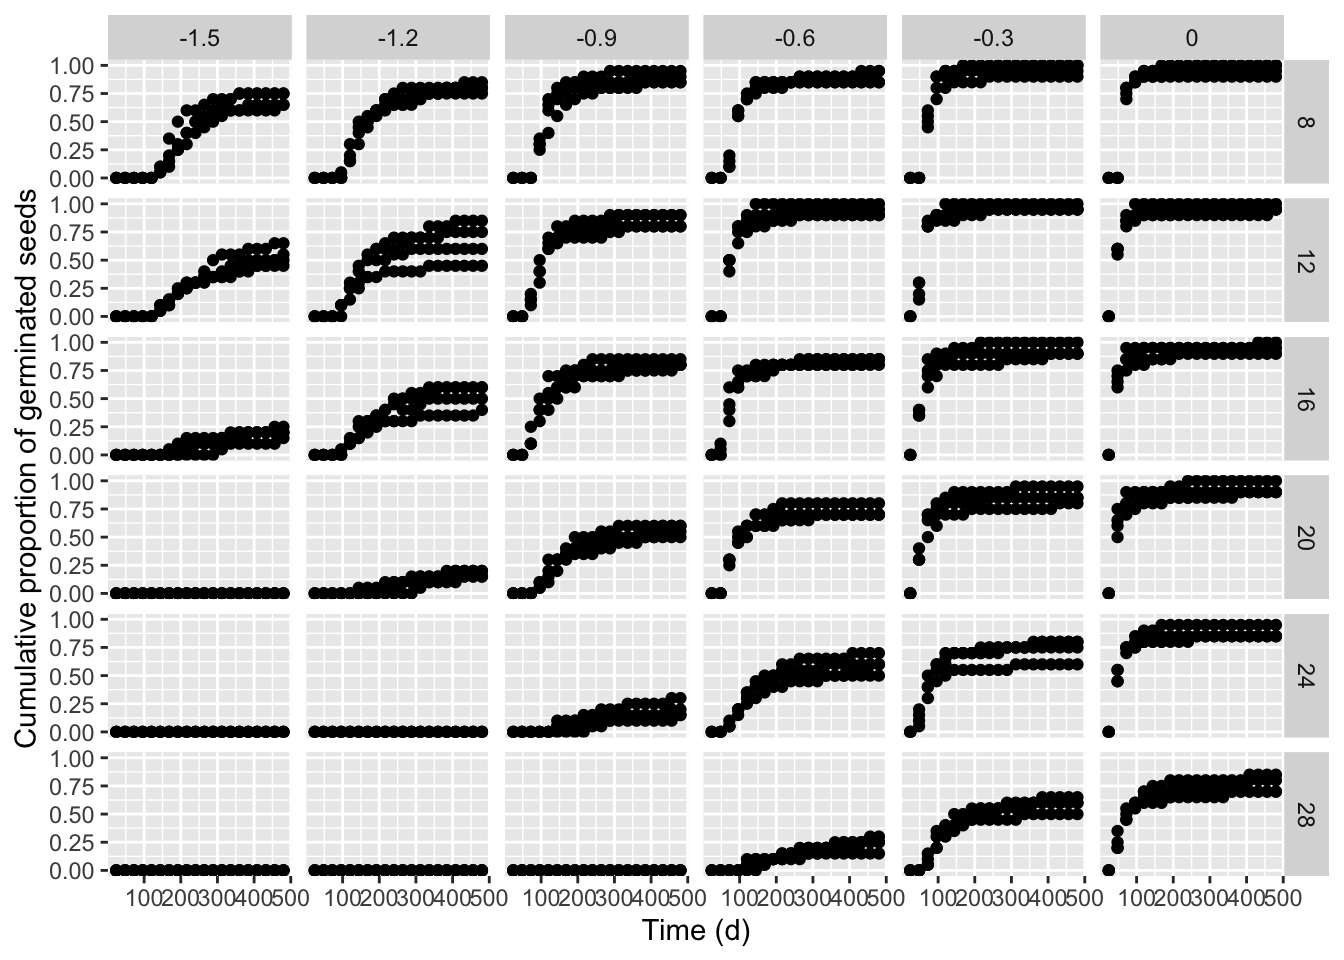
\includegraphics{_main_files/figure-latex/unnamed-chunk-74-1.pdf}

Questo dataset mostra una chiara eteroscedasticità. Utilizziamo quindi
la funzione `boxcox()' per individuare la trasformazione più adatta a
correggere questa patologia.

\begin{Shaded}
\begin{Highlighting}[]
\NormalTok{MASS}\OperatorTok{::}\KeywordTok{boxcox}\NormalTok{(mod)}
\end{Highlighting}
\end{Shaded}

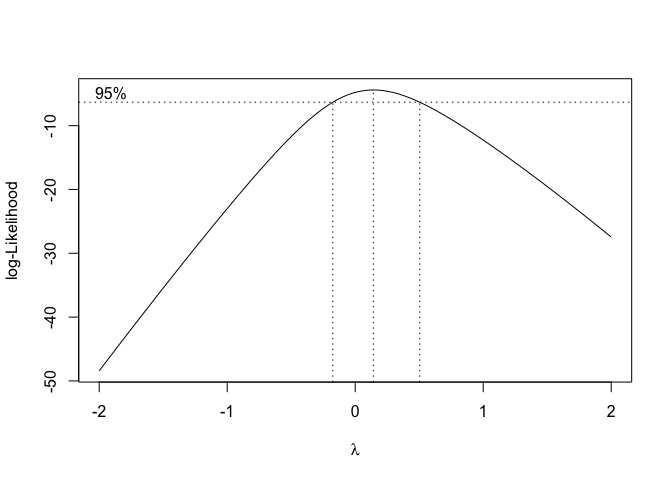
\includegraphics{_main_files/figure-latex/unnamed-chunk-75-1.pdf}

Dal grafico si individua chiaramente che la trasformazione migliore,
scelta tra quelle più semplici e comprensibili, è quella che corrisponde
a \(\lambda = 0\), cioè la trasformazione logaritmica.

\begin{Shaded}
\begin{Highlighting}[]
\NormalTok{mod <-}\StringTok{ }\KeywordTok{lm}\NormalTok{(}\KeywordTok{log}\NormalTok{(Count) }\OperatorTok{~}\StringTok{ }\NormalTok{Insecticide, }\DataTypeTok{data =}\NormalTok{ insects)}
\KeywordTok{plot}\NormalTok{(mod, }\DataTypeTok{which =} \DecValTok{1}\NormalTok{)}
\end{Highlighting}
\end{Shaded}

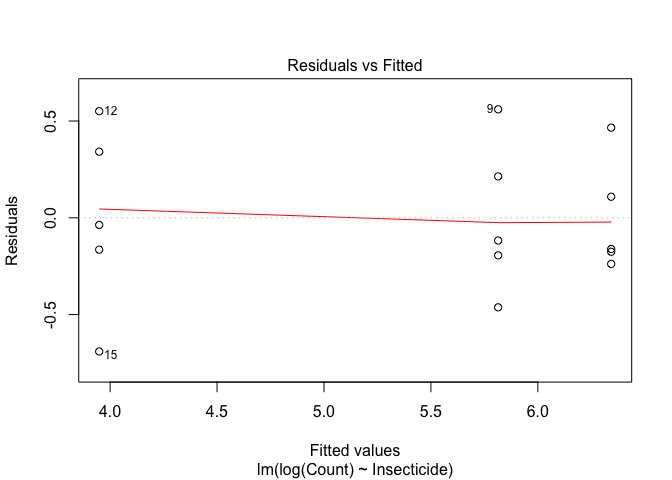
\includegraphics{_main_files/figure-latex/unnamed-chunk-76-1.pdf}

Vediamo che i dati trasformati non mostrano più alcun sintomo di
eteroscedasticità e, di conseguenza, l'ANOVA su questa metrica è
affidabile.

Ovviamente, vi sarà la complicazione che i risultati dovranno essere
commentati nella scala trasformata e quindi la loro interpretazione
risulterà più complicata.

\section{Referenze bibliografiche per
approfondimenti}\label{referenze-bibliografiche-per-approfondimenti}

Ahrens, W. H., D. J. Cox, and G. Budwar. 1990, Use of the arcsin and
square root trasformation for subjectively determined percentage data.
Weed science 452-458.\\
Anscombe, F. J. and J. W. Tukey. 1963, The examination and analysis of
residuals. Technometrics 5: 141-160.\\
Babbini, M., B. Chiandotto, G. Chisci, R. d. Cristofaro, G. A.
Maccararo, N. Montanaro, F. Nicolis, E. Ottaviano, F. Salvi, and M.
Turri. 1978. Biometria: principi e metodi per studenti e ricercatori
biologi. Padova: P. 552.\\
Box, G. E. P. and D. R. Cox. 1964, An analysis of transformations.
Journal of the Royal Statistical Society, B-26, 211-243, discussion
244-252.\\
Camussi , A., F. Moller , E. Ottaviano , and M. Sarli Gorla . 1986,
Metodi statistici per la sperimentazione biologica. Ed. Zanichelli.\\
Chatfield, C. 1985, The initial examination of data. J. R. Statist. Soc.
A-148, 3, 214-253 A-148: 214-253.\\
D'Elia, A. 2001, Un metodo grafico per la trasformazione di Box-Cox:
aspetti esplorativi ed inferenziali. STATISTICA LXI: 630-648.\\
Draper, N. R. and H. Smith. 1981, Applied regression. John Wiley \&
Sons, Inc. , New York, 2nd ed.\\
Saskia, R. M. 1992, The Box-Cox transformation technique: a review.
Statistician 41: 169-178.\\
Snedecor, G. W. and W. G. Cochran. 1991. Statistical methods. AMES
(Iowa): IOWA State University Press, VIII Edition. P. 503.\\

\chapter{Modelli lineari con più variabili
indipendenti}\label{modelli-lineari-con-piu-variabili-indipendenti}

\section{Introduzione}\label{introduzione-3}

Nel capitolo precedente abbiamo visto come è possibile costruire modelli
nei quali abbiamo una sola variabile dipendente quantitativa e una
variabile indipendente categorica. Abbiamo anche visto che questo tipo
di modelli lineari sono normalmente noti come modelli `ANOVA'.
Ovviamente è possibile definire modelli analoghi, ma più complessi,
caratterizzati da più di una variabile indipendente categorica, con i
quali è possibile descrivere i risultati di esperimenti
multi-fattoriali. Vediamo ora alcuni esempi

\section{ANOVA a blocchi
randomizzati}\label{anova-a-blocchi-randomizzati}

Abbiamo una prova di confronto tra erbicidi in mais, con 13 formulati,
due testimoni inerbiti (che, per comodità, considereremo due trattamenti
diversi) e un testimone scerbato. Date le dimensioni della prova, è
lecito ipotizzare che, pur scegliendo un appezzamento il più omogeneo
possibile, ci potrebbero essere differenze di infestazione tra un punto
e l'altro del campo, con un presumibile gradiente procedendo dai lati
(vicino alle fosse) verso il centro. In questa situazione, se
l'esperimento fosse disegnato a randomizzazione completa, le differenze
di infestazione tra una parte e l'altra del campo sarebbero trascurate e
finirebbero per incrementare l'errore sperimentale, diminuendo
l'efficienza dell'esperimento.

Si impiega quindi un disegno a blocchi randomizzati con quattro
repliche. Ricordiamo che, con questo disegno, il campo è suddiviso in
tante sezioni (dette blocchi) quante sono le repliche (quattro),
perpendicolarmente al gradiente di infestazione trasversale. In questo
modo, l'ambiente è relativamente omogeneo all'interno di ciascun blocco
nel quale si è collocata una replica per trattamento.

Il dataset dei risultati (`rimsulfuron') è contenuto nel package
`aomisc'; consideriamo come variabile risposta la produzione (`Yield').

\begin{Shaded}
\begin{Highlighting}[]
\KeywordTok{library}\NormalTok{(aomisc)}
\KeywordTok{library}\NormalTok{(reshape)}
\KeywordTok{data}\NormalTok{(rimsulfuron)}
\end{Highlighting}
\end{Shaded}

La produzione di ogni unità sperimentale (parcella) è condizionata da
più di un effetto:

\begin{enumerate}
\def\labelenumi{\arabic{enumi}.}
\tightlist
\item
  il diserbante con cui essa è stata trattata;
\item
  il blocco di cui essa fa parte;
\item
  ogni altro effetto non conoscibile e puramente casuale.
\end{enumerate}

Il modello è quindi:

\[ Y_{ij} = \mu + \gamma_i + \alpha_j + \varepsilon_{ij}\]

dove \(Y\) è la produzione nel blocco \(i\) e con il diserbo \(j\),
\(\mu\) è l'intercetta, \(\gamma\) è l'effetto del blocco \(i\),
\(\alpha\) è l'effetto del trattamento \(j\) e \(\varepsilon\) è
l'errore sperimentale per ogni singola parcella, che si assume
normalmente distribuito, con media 0 e deviazione standard \(\sigma\).
Per gli usuali problemi di stimabilità, poniamo i vincoli
\(\gamma_1 = 0\) e \(\alpha_1 = 0\) (vincolo sul trattamento), in modo
che \(\mu\) rappresenta il valore atteso nel primo blocco e per il primo
trattamento in ordine alfabetico. In totale, vi sono 19 parametri da
stimare, più \(\sigma\).

La stima dei parametri viene eseguita con il metodo dei minimi quadrati.
Per motivi didattici, costruiamo il modello in modo incrementale,
inserendo gli effetti uno alla volta nel modello. Il primo modello è
quindi quello che contiene la sola intercetta e il residuo:

\begin{Shaded}
\begin{Highlighting}[]
\NormalTok{mod1 <-}\StringTok{ }\KeywordTok{lm}\NormalTok{(Yield }\OperatorTok{~}\StringTok{ }\DecValTok{1}\NormalTok{, }\DataTypeTok{data =}\NormalTok{ rimsulfuron)}
\NormalTok{RSS1 <-}\StringTok{ }\KeywordTok{sum}\NormalTok{( }\KeywordTok{residuals}\NormalTok{(mod1)}\OperatorTok{^}\DecValTok{2}\NormalTok{ )}
\NormalTok{RSS1}
\NormalTok{## [1] 53779.07}
\end{Highlighting}
\end{Shaded}

Di questo modello, calcoliamo la somma dei quadrati dei residui
(devianza del residuo), che è visibile più sopra.

In seconda battuta, inseriamo l'effetto blocco:

\begin{Shaded}
\begin{Highlighting}[]
\NormalTok{mod2 <-}\StringTok{ }\KeywordTok{lm}\NormalTok{(Yield }\OperatorTok{~}\StringTok{ }\KeywordTok{factor}\NormalTok{(Block), }\DataTypeTok{data =}\NormalTok{ rimsulfuron)}
\NormalTok{RSS2 <-}\StringTok{ }\KeywordTok{sum}\NormalTok{( }\KeywordTok{residuals}\NormalTok{(mod2)}\OperatorTok{^}\DecValTok{2}\NormalTok{ )}
\NormalTok{RSS2}
\NormalTok{## [1] 51118.58}
\end{Highlighting}
\end{Shaded}

Vediamo che la devianza del residuo è calata di \texttt{RSS1\ -\ RSS2}
unità, che corrispondono all'effetto del blocco e alla sua introduzione
nel modello.

Infine, inseriamo anche l'effetto del trattamento:

\begin{Shaded}
\begin{Highlighting}[]
\NormalTok{mod3 <-}\StringTok{ }\KeywordTok{lm}\NormalTok{(Yield }\OperatorTok{~}\StringTok{ }\KeywordTok{factor}\NormalTok{(Block) }\OperatorTok{+}\StringTok{ }\KeywordTok{factor}\NormalTok{(Code),}
           \DataTypeTok{data =}\NormalTok{ rimsulfuron)}
\NormalTok{RSS3 <-}\StringTok{ }\KeywordTok{sum}\NormalTok{( }\KeywordTok{residuals}\NormalTok{(mod3)}\OperatorTok{^}\DecValTok{2}\NormalTok{ )}
\NormalTok{RSS3}
\NormalTok{## [1] 7187.348}
\end{Highlighting}
\end{Shaded}

L'inserimento di quest'ultimo effetto ha determinato un calo della
devianza del residuo pari \texttt{RSS2\ -\ RSS3}, che corrisponde
appunto all'effetto del diserbo. Insomma, ogni effetto introdotto nel
modello ha determinato un decremento della variabilità non spiegata,
quantitativamente pari alla variabilità attribuibile all'effetto stesso.
Alla fine del processo rimane comunque un certo residuo (RSS3) non
spiegato, cioè \(\varepsilon\).

Ci chiediamo se gli effetti attribuibili al blocco e al trattamento sono
significativamente più grandi del residuo. Sappiamo già di non poter
confrontare le devianze, ma possiamo calcolare e confrontare con un test
di F le relative varianze. Basta tener conto che i gradi di libertà dei
blocchi e dei trattamenti sono rispettivamente 3 e 15, cioè il numero
dei blocchi meno uno e il numero dei trattamenti meno uno.

La tabella ANOVA può essere facilmente ottenuta con R:

\begin{Shaded}
\begin{Highlighting}[]
\KeywordTok{anova}\NormalTok{(mod3)}
\NormalTok{## Analysis of Variance Table}
\NormalTok{## }
\NormalTok{## Response: Yield}
\NormalTok{##               Df Sum Sq Mean Sq F value    Pr(>F)    }
\NormalTok{## factor(Block)  3   2660  886.83  5.5524  0.002496 ** }
\NormalTok{## factor(Code)  15  43931 2928.75 18.3369 2.329e-14 ***}
\NormalTok{## Residuals     45   7187  159.72                      }
\NormalTok{## ---}
\NormalTok{## Signif. codes:  0 '***' 0.001 '**' 0.01 '*' 0.05 '.' 0.1 ' ' 1}
\end{Highlighting}
\end{Shaded}

Ovviamente, prima di considerare questa tabella dovremo preoccuparci del
fatto che le assunzioni di base siano rispettate, cosa che possiamo
facilmente verificare con un'analisi grafica dei residui.

\begin{Shaded}
\begin{Highlighting}[]
\KeywordTok{par}\NormalTok{(}\DataTypeTok{mfrow=}\KeywordTok{c}\NormalTok{(}\DecValTok{1}\NormalTok{,}\DecValTok{2}\NormalTok{))}
\KeywordTok{plot}\NormalTok{(mod3, }\DataTypeTok{which =} \DecValTok{1}\NormalTok{)}
\KeywordTok{plot}\NormalTok{(mod3, }\DataTypeTok{which =} \DecValTok{2}\NormalTok{)}
\end{Highlighting}
\end{Shaded}

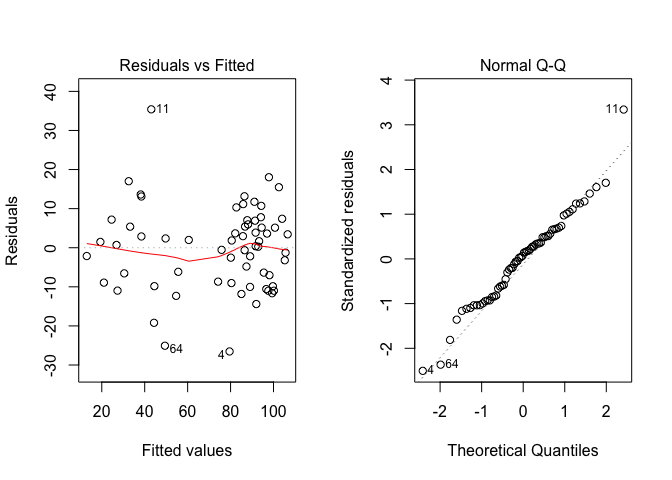
\includegraphics{_main_files/figure-latex/unnamed-chunk-83-1.pdf}

Dopo esserci rassicurati su questo importante aspetto, possiamo vedere
che abbiamo due ipotesi nulle da testare (effetto del trattamento non
significativo ed effetto del blocco non significativo), che possono
essere entrambe rifiutate per P \textless{} 0.05.

\section{ANOVA a quadrato latino}\label{anova-a-quadrato-latino}

Immaginiamo di voler studiare il tempo necessario per costruire un
componente elettronico, utilizzando quattro metodi diversi. E' evidente
che il tempo di costruzione sarà influenzato dalla perizia del tecnico
e, per questo, utilizziamo quattro tecnici diversi, ad ognuno dei quali
facciamo utilizzare tutti e quattro i metodi. Un esperimento così
disegnato sarebbe a blocchi randomizzati, con il tecnico che fa da
blocco per i trattamenti. Tuttavia, dobbiamo anche riconoscere che i
quattro tecnici saranno via via meno efficienti, e quindi il metodo che
utilizzeranno per primo sarà avvantaggiato, mentre quello che
utilizzeranno per ultimo sarà svantaggiato. E'vero che i metodi sono
assegnati in ordine random ad ogni tecnico, ma non si può comunque
evitare che un metodo venga avvantaggiato rispetto ad un altro, perché,
ad esempio, non viene mai ad occupare l'ultima posizione (o meglio,
l'ultimo turno).

Per evitare questo problema imponiamo un vincolo ulteriore alla
randizzazione e facciamo in modo che ogni metodo occupi tutte e quattro
i turni, in tecnici diversi. Il disegno è quindi a quadrato latino.

Il dataset dei risultati è disponibile su gitHub:

\begin{Shaded}
\begin{Highlighting}[]
\NormalTok{dataset <-}\StringTok{ }\KeywordTok{read.csv}\NormalTok{(}\StringTok{"https://raw.githubusercontent.com/OnofriAndreaPG/aomisc/master/data/Technicians.csv"}\NormalTok{, }\DataTypeTok{header=}\NormalTok{T)}
\NormalTok{dataset}
\NormalTok{##    Shift Technician Method Time}
\NormalTok{## 1      I     Andrew      C   90}
\NormalTok{## 2     II     Andrew      B   90}
\NormalTok{## 3    III     Andrew      A   89}
\NormalTok{## 4     IV     Andrew      D  104}
\NormalTok{## 5      I       Anna      D   96}
\NormalTok{## 6     II       Anna      C   91}
\NormalTok{## 7    III       Anna      B   97}
\NormalTok{## 8     IV       Anna      A  100}
\NormalTok{## 9      I    Michael      A   84}
\NormalTok{## 10    II    Michael      D   96}
\NormalTok{## 11   III    Michael      C   98}
\NormalTok{## 12    IV    Michael      B  104}
\NormalTok{## 13     I      Sarah      B   88}
\NormalTok{## 14    II      Sarah      A   88}
\NormalTok{## 15   III      Sarah      D   98}
\NormalTok{## 16    IV      Sarah      C  106}
\end{Highlighting}
\end{Shaded}

In questo caso abbiamo un trattamento (metodo) e due effetti `blocco'
(tecnico e turno), che debbono tutti essere inclusi nel modello, che può
essere così definito:

\[Y_{ijk} = \mu + \gamma_k + \beta_j + \alpha_i + \varepsilon_{ijk}\]

dove \(\mu\) è l'intercetta, \(\gamma\) è l'effetto del turno k,
\(\beta\) è l'effetto del tecnico j e \(\alpha\) è l'effetto del metodo
i. L'elemento \(\varepsilon_{ijk}\) rappresenta la componente random
individuale, di ogni osservazione e si assume normalmente distribuita,
con media 0 e deviazione standard \(\sigma\).

Avendo già illustrato il processo di sviluppo incrementale del modello e
quindi utilizziamo subito R e il metodo dei minimi quadrati per la stima
dei parametri:

\begin{Shaded}
\begin{Highlighting}[]
\NormalTok{mod <-}\StringTok{ }\KeywordTok{lm}\NormalTok{(Time }\OperatorTok{~}\StringTok{ }\NormalTok{Method }\OperatorTok{+}\StringTok{ }\NormalTok{Technician}
          \OperatorTok{+}\StringTok{ }\NormalTok{Shift, }\DataTypeTok{data =}\NormalTok{ dataset)}
\end{Highlighting}
\end{Shaded}

Verifichiamo il rispetto delle assunzioni di base, con l'analisi grafica
dei residui.

\begin{Shaded}
\begin{Highlighting}[]
\KeywordTok{par}\NormalTok{(}\DataTypeTok{mfrow=}\KeywordTok{c}\NormalTok{(}\DecValTok{1}\NormalTok{,}\DecValTok{2}\NormalTok{))}
\KeywordTok{plot}\NormalTok{(mod, }\DataTypeTok{which =} \DecValTok{1}\NormalTok{)}
\KeywordTok{plot}\NormalTok{(mod, }\DataTypeTok{which =} \DecValTok{2}\NormalTok{)}
\end{Highlighting}
\end{Shaded}

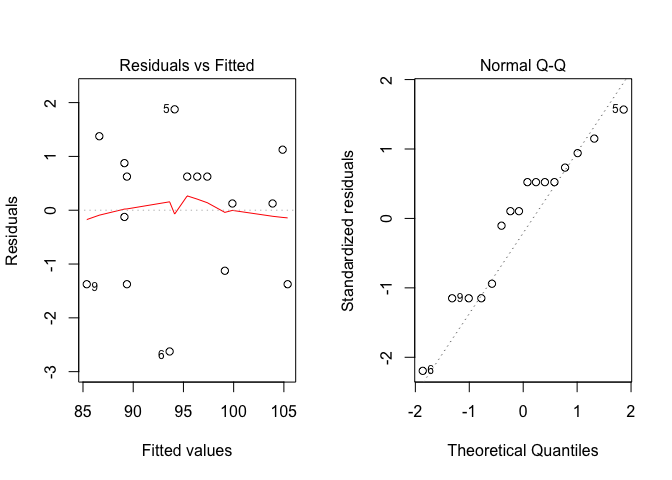
\includegraphics{_main_files/figure-latex/unnamed-chunk-86-1.pdf}

Non essendovi evidenti problemi, valutiamo la significatività degli
effetti nel modello, analogamente a quanto abbiamo fatto nel caso
dell'ANOVA a blocchi randomizzati. L'unica differenza sta nel fatto che,
nei disegni a quadrato latino, vi sono tre effetti da testare, anche se
l'unico ad avere una certa rilevanza è l'effetto del metodo di lavoro.

\begin{Shaded}
\begin{Highlighting}[]
\KeywordTok{anova}\NormalTok{(mod)}
\NormalTok{## Analysis of Variance Table}
\NormalTok{## }
\NormalTok{## Response: Time}
\NormalTok{##            Df Sum Sq Mean Sq F value    Pr(>F)    }
\NormalTok{## Method      3 145.69  48.563 12.7377 0.0051808 ** }
\NormalTok{## Technician  3  17.19   5.729  1.5027 0.3065491    }
\NormalTok{## Shift       3 467.19 155.729 40.8470 0.0002185 ***}
\NormalTok{## Residuals   6  22.87   3.812                      }
\NormalTok{## ---}
\NormalTok{## Signif. codes:  0 '***' 0.001 '**' 0.01 '*' 0.05 '.' 0.1 ' ' 1}
\end{Highlighting}
\end{Shaded}

Vediamo che esiste una differenza significativa tra i metodi e l'ipotesi
nulla può essere rifiutata con una bassissima probabilità di errore di
prima specie.

\chapter{Contrasti e confronti multipli con
R}\label{contrasti-e-confronti-multipli-con-r}

\section{Introduzione}\label{introduzione-4}

L'ANOVA rappresenta frequentemente il primo passo nell'elaborazione
statistica dei dati sperimentali. Essa consente di quantificare l'errore
sperimentale e ci permette di sapere se l'effetto del trattamento (nel
suo complesso) è risultato significativo. Tuttavia, con la sola ANOVA
non siamo ancora capaci di definire una graduatoria di merito tra i
diversi livelli del trattamento sperimentale. Dopo l'ANOVA è quindi
logico chiedersi (in ordine crescente di importanza):

\begin{enumerate}
\def\labelenumi{\arabic{enumi}.}
\tightlist
\item
  Il generico trattamento A ha un effetto diverso dal trattamento B?
\item
  Il trattamento A è migliore/uguale/peggiore di B?
\item
  Quant'è la differenza tra A e B?
\end{enumerate}

La prima domanda è abbastanza sciocca, in quanto due trattamenti non
sono quasi mai esattamente uguali. Le altre due domande sono invece più
rilevanti, specialmente la seconda, in quanto conoscere l'entità della
differenza, oltre che la sua significatività, è fondamentale per
comprendere anche la sua rilevanza biologica. Infatti una differenza
potrebbe essere significativa, ma irrilevante da un punto di vista
agronomico o, viceversa, essa potrebbe essere non significativa, ma
estremamente rilevante, quindi meritevole di ulteriori approfondimenti
scientifici. Per rispondere alle domande precedenti in genere
utilizziamo i contrasti e i confronti multipli, che introdurremo con un
esempio.

\section{Esempio}\label{esempio}

Ammettiamo di aver effettuato una prova con un trattamento sperimentali
caratterizzato da quattro livelli qualitativi (tesi di concimazione),
con i risultati riportati di seguito:

\begin{Shaded}
\begin{Highlighting}[]
\NormalTok{yield <-}\StringTok{ }\KeywordTok{c}\NormalTok{(}\DecValTok{20}\NormalTok{,}\DecValTok{21}\NormalTok{,}\DecValTok{23}\NormalTok{,}\DecValTok{22}\NormalTok{,}\DecValTok{19}\NormalTok{,}\DecValTok{20}\NormalTok{,}\DecValTok{12}\NormalTok{,}\DecValTok{15}\NormalTok{,}\DecValTok{13}\NormalTok{,}\DecValTok{19}\NormalTok{,}\DecValTok{18}\NormalTok{,}\DecValTok{16}\NormalTok{)}
\NormalTok{fert <-}\StringTok{ }\KeywordTok{factor}\NormalTok{(}\KeywordTok{rep}\NormalTok{(}\KeywordTok{c}\NormalTok{(}\StringTok{"Minerale"}\NormalTok{, }\StringTok{"Minerale lento"}\NormalTok{, }
          \StringTok{"Non concimato"}\NormalTok{, }\StringTok{"Organico"}\NormalTok{), }\DataTypeTok{each=}\DecValTok{3}\NormalTok{))}
\NormalTok{dataset <-}\StringTok{ }\KeywordTok{data.frame}\NormalTok{(yield, fert)}
\KeywordTok{rm}\NormalTok{(yield, fert)}
\NormalTok{dataset}
\NormalTok{##    yield           fert}
\NormalTok{## 1     20       Minerale}
\NormalTok{## 2     21       Minerale}
\NormalTok{## 3     23       Minerale}
\NormalTok{## 4     22 Minerale lento}
\NormalTok{## 5     19 Minerale lento}
\NormalTok{## 6     20 Minerale lento}
\NormalTok{## 7     12  Non concimato}
\NormalTok{## 8     15  Non concimato}
\NormalTok{## 9     13  Non concimato}
\NormalTok{## 10    19       Organico}
\NormalTok{## 11    18       Organico}
\NormalTok{## 12    16       Organico}
\end{Highlighting}
\end{Shaded}

L'ANOVA può essere eseguita facilmente con R o con un altro software.

\begin{Shaded}
\begin{Highlighting}[]
\NormalTok{model <-}\StringTok{ }\KeywordTok{lm}\NormalTok{(yield }\OperatorTok{~}\StringTok{ }\NormalTok{fert, }\DataTypeTok{data=}\NormalTok{dataset)}
\KeywordTok{anova}\NormalTok{(model)}
\NormalTok{## Analysis of Variance Table}
\NormalTok{## }
\NormalTok{## Response: yield}
\NormalTok{##           Df  Sum Sq Mean Sq F value    Pr(>F)    }
\NormalTok{## fert       3 115.000  38.333  16.429 0.0008821 ***}
\NormalTok{## Residuals  8  18.667   2.333                      }
\NormalTok{## ---}
\NormalTok{## Signif. codes:  0 '***' 0.001 '**' 0.01 '*' 0.05 '.' 0.1 ' ' 1}
\end{Highlighting}
\end{Shaded}

In questo caso, l'analisi della varianza ed il relativo test di F ci
dicono che esiste una differenza significativa tra le medie, ma rimane
il problema di classificare le soluzioni concimanti in ordine di
efficacia. Per calcolare le medie dei trattamenti utilizziamo la
funzione \emph{emmeans()} del package \emph{emmeans}:

\begin{Shaded}
\begin{Highlighting}[]
\KeywordTok{library}\NormalTok{(emmeans)}
\KeywordTok{library}\NormalTok{(multcomp)}
\NormalTok{medie <-}\StringTok{ }\KeywordTok{emmeans}\NormalTok{(model, }\OperatorTok{~}\NormalTok{fert)}
\NormalTok{medie}
\NormalTok{##  fert             emmean        SE df lower.CL upper.CL}
\NormalTok{##  Minerale       21.33333 0.8819171  8 19.29963 23.36704}
\NormalTok{##  Minerale lento 20.33333 0.8819171  8 18.29963 22.36704}
\NormalTok{##  Non concimato  13.33333 0.8819171  8 11.29963 15.36704}
\NormalTok{##  Organico       17.66667 0.8819171  8 15.63296 19.70037}
\NormalTok{## }
\NormalTok{## Confidence level used: 0.95}
\end{Highlighting}
\end{Shaded}

Vediamo che l'output di R riporta anche gli errori standard delle medie
(SEM) e gli intervalli di confidenza.

\section{I contrasti}\label{i-contrasti}

Si definisce CONTRASTO una combinazione lineare dei parametri di un
modello (ad esempio le medie dei trattamenti), in modo che i
coefficienti sommati diano 0. Ad esempio, considerando i parametri del
modello precedente, una combinazione lineare del tipo:

\[ C = \frac{1}{3} \cdot 21.33 + \frac{1}{3} \cdot 20.33 - 1 \cdot 13.33 + \frac{1}{3} \cdot 17.67 = 6.446667\]

è un contrasto, in quanto i coefficienti sommati 1/3 + 1/3 - 1 + 1/3 =
0. Al contrario una combinazione del tipo:

\[C1 = 1 \cdot 21.33  + 1 \cdot 20.33 - 1 \cdot 13.33 + 1 \cdot 17.67\]

non è un contrasto valido, perché la somma dei coefficienti non è zero
(1 + 1 - 1 + 1 = -2).

Il primo contrasto C, ha un preciso significato biologico, in quanto
stima la differenza tra il non fertilizzato e la media dei fertilizzati
e risponde a tutte e tre le domande:

\begin{enumerate}
\def\labelenumi{\arabic{enumi}.}
\tightlist
\item
  La fertilizzazione (in media) ha un effetto diverso dal testimone non
  fertilizzato? Risposta: si, perché la differenza è non nulla
\item
  La fertilizzazione in media è migliore/uguale/peggiore del testimone?
  Risposta: migliore, perché la differenza è positiva.
\item
  Quant'è la differenza tra il fertilizzato e il non-fertilizzato?
  Risposta: è pari a 6.45
\end{enumerate}

E' evidente, tuttavia, che l'errore sperimentale produce incertezza, che
sarebbe bene includere nei risultati, sotto forma di intervallo di
confidenza. La domanda quindi è: qual è la varianza del contrasto?

\subsection{Varianza del contrasto e intervalli di
confidenza}\label{varianza-del-contrasto-e-intervalli-di-confidenza}

Ogni contrasto ha la sua varianza, ottenuta come combinazione lineare di
varianze, attraverso il metodo di propagazione degli errori. In
generale:

\[var(A x + B y) = A^{2} var(x) + B^2 var(y) + 2 A \times B \,\, covar (x y)\]

dove A e B sono i coefficienti del contrasto, x e y sono i parametri del
modello. Se i parametri non sono correlati (come in questo caso e, in
genere, nell'ANOVA) la covarianza è zero e quindi la varianza della
somma/differenza è uguale alla somma delle varianze.

Nel nostro caso, la varianza del contrasto è:

\[var(C) = \left( \frac{1}{3} \cdot 0.882 \right)^2 +  \left( \frac{1}{3} \cdot 0.882 \right)^2 + 0.882^2 +  \left( \frac{1}{3} \cdot 0.882 \right)^2 = 1.037\]

mentre la deviazione standard è pari ad 1.0183. Dopo aver calcolato la
deviazione standard, possiamo costruire un intervallo di confidenza per
il contrasto, utilizzando le formule usuali (quantili della
distribuzione di t):

\begin{Shaded}
\begin{Highlighting}[]
\NormalTok{limSup <-}\StringTok{ }\FloatTok{6.4467} \OperatorTok{+}\StringTok{ }\KeywordTok{qt}\NormalTok{(}\FloatTok{0.975}\NormalTok{, }\DecValTok{8}\NormalTok{) }\OperatorTok{*}\StringTok{ }\FloatTok{1.018277}
\NormalTok{limInf <-}\StringTok{ }\FloatTok{6.4467} \OperatorTok{-}\StringTok{ }\KeywordTok{qt}\NormalTok{(}\FloatTok{0.975}\NormalTok{, }\DecValTok{8}\NormalTok{) }\OperatorTok{*}\StringTok{ }\FloatTok{1.018277}
\NormalTok{limInf; limSup}
\NormalTok{## [1] 4.098549}
\NormalTok{## [1] 8.794851}
\end{Highlighting}
\end{Shaded}

Con questo abbiamo risposto a tutte e tre le nostre domande di ricerca:

\begin{enumerate}
\def\labelenumi{\arabic{enumi}.}
\tightlist
\item
  Fertilizzare non produce lo stesso effetto che non fertilizzare;
\item
  Fertilizzare permette di produrre di più che non fertilizzare.
\item
  La differenza è pari a 6.44 q/ha e, ripetendo questo esperimento, nel
  95\% dei casi otterremo differenze variabili entro l'intervallo tra
  4.1 e 8.8 q/ha.
\end{enumerate}

\subsection{Significatività del contrasto e intervalli di
confidenza}\label{significativita-del-contrasto-e-intervalli-di-confidenza}

E' importante notare che l'intervallo di confidenza esposto in
precedenza non contiene lo zero e quindi la differenza tra i due
trattamenti in studio è significativa (significativamente diversa da 0).
Tuttavia potremmo essere intenzionati a testare questa differenza in
modo formale, a prescindere dal calcolo dell'intervallo di confidenza.
Secondo Tukey (1991), questo tipo di test è sciocco (`foolish') almeno
per due motivi:

\begin{enumerate}
\def\labelenumi{\arabic{enumi}.}
\tightlist
\item
  la domanda non è realistica: due trattamenti diversi non possono che
  dare risultati diversi, magari in modo impercettibile, ma pur sempre
  diversi;
\item
  l'eventuale rifiuto dell'ipotesi nulla non ci da nessuna informazione
  sulla rilevanza biologica della differenza, che è indipendente dalla
  sua significatività.
\end{enumerate}

Ferma restando l'importanza dell'intervallo di confidenza, quale misura
della \emph{effect size}, il test d'ipotesi è pratica usuale e quindi la
tratteremo nel dovuto dettaglio. Dovrebbe essere noto che il rapporto
tra una stima ed il suo errore standard ha una distribuzione di t di
Student, con un numero di gradi di libertà pari all'errore. Di
conseguenza possiamo saggiare l'ipotesi nulla che il contrasto è uguale
a 0 calcolando la probabilità di trovare un valore di t pari o superiore
(in valore assoluto) a quello da noi ottenuto. Nell'esempio sottostante
abbiamo moltiplicato la probabilità trovata per 2, dato che si tratta di
un test a due code:

\begin{Shaded}
\begin{Highlighting}[]
\NormalTok{t <-}\StringTok{ }\FloatTok{6.4467} \OperatorTok{/}\StringTok{ }\FloatTok{1.018277}
\DecValTok{2} \OperatorTok{*}\StringTok{ }\KeywordTok{pt}\NormalTok{(t, }\DecValTok{8}\NormalTok{, }\DataTypeTok{lower.tail =}\NormalTok{ F)}
\NormalTok{## [1] 0.0002251554}
\end{Highlighting}
\end{Shaded}

\subsection{I contrasti con R}\label{i-contrasti-con-r}

Nel caso in esempio, si potrebbero pianificare tre contrasti (incluso
quello già discusso):

\begin{enumerate}
\def\labelenumi{\arabic{enumi}.}
\tightlist
\item
  non concimato vs concimato (in media)
\item
  concime organico vs.~concimi minerali (in media)
\item
  minerale tradizionale vs.~lento rilascio.
\end{enumerate}

Eseguire questi contrasti con R è abbastanza semplice, utilizzando il
package \emph{emmeans}. La procedura di lavoro è la seguente:

\begin{enumerate}
\def\labelenumi{\arabic{enumi}.}
\tightlist
\item
  adattare il modello e stimarne i parametri (funzione lm(), utilizzata
  più sopra)
\item
  costruire un vettore per ogni contrasto, contenente i relativi
  coefficienti, tenendo presente l'ordine delle medie nell'oggetto
  `medie' (m1, m2, m3; vedi più sotto)
\item
  Impiegare la funzione \emph{contrast}, passandole come argomento
  l'oggetto `medie' ottenuto con la funzione \emph{emmeans} (vedi sopra)
  ed una lista contenente i tre vettori dei coefficienti (m1, m2, m3),
  ai quali si può assegnare un nome, ad esempio, C1, C2 e C3.
\item
  Con la funzione \emph{confint} possiamo ottenere gli intervalli di
  confidenza, invece che le significanze.
\end{enumerate}

\small

\begin{verbatim}
m1 <- c(1/3, 1/3,  -1, 1/3)
m2 <- c(0.5, 0.5, 0, -1)
m3 <- c(1, -1, 0, 0)
contrast(medie, method=list(C1=m1, C2=m2, C3=m3), 
           adjust="none")
confint(contrast(medie, method=list(C1=m1, C2=m2, C3=m3), 
           adjust="none"))
\end{verbatim}

\normalsize

Il test mostra che la concimazione ha, in media, un effetto
significativo, che il concime organico differisce significativamente dai
minerali (in media) e che il concime a lento rilascio non è
significativamente diverso da quello normale.

\section{I confronti multipli a coppie (pairwise
comparisons)}\label{i-confronti-multipli-a-coppie-pairwise-comparisons}

Non sempre le prove sperimentali consentono di saggiare pochi contrasti
pre-stabiliti, ma spesso è necessario confrontare tutte le possibili
coppie di trattamenti (\emph{pairwise comparisons}). In questo caso
dovremmo definire un contrasto per ogni coppia di medie, anche se
l'impiego del package \emph{emmeans} agevola, non di poco, il lavoro.

In particolare, possiamo immaginare due situazioni di riferimento: tutti
contro tutti (confronti tipo ``Tukey'') e tutti verso uno (confronti
tipo ``Dunnett'').

Nell'esempio sottostante mostriamo un confronto tipo Tukey (tutti contro
tutti), eseguito utilizzando la funzione `contrast' (come sopra),
passando il valore `pairwise' all'argomento `method'.

\footnotesize

\begin{Shaded}
\begin{Highlighting}[]
\CommentTok{#Confronti multipli a coppie}
\KeywordTok{contrast}\NormalTok{(medie, }\DataTypeTok{adjust=}\StringTok{"none"}\NormalTok{, }\DataTypeTok{method=}\StringTok{"pairwise"}\NormalTok{)}
\NormalTok{##  contrast                        estimate       SE df t.ratio p.value}
\NormalTok{##  Minerale - Minerale lento       1.000000 1.247219  8   0.802  0.4458}
\NormalTok{##  Minerale - Non concimato        8.000000 1.247219  8   6.414  0.0002}
\NormalTok{##  Minerale - Organico             3.666667 1.247219  8   2.940  0.0187}
\NormalTok{##  Minerale lento - Non concimato  7.000000 1.247219  8   5.612  0.0005}
\NormalTok{##  Minerale lento - Organico       2.666667 1.247219  8   2.138  0.0650}
\NormalTok{##  Non concimato - Organico       -4.333333 1.247219  8  -3.474  0.0084}
\KeywordTok{confint}\NormalTok{(}\KeywordTok{contrast}\NormalTok{(medie, }\DataTypeTok{adjust=}\StringTok{"none"}\NormalTok{, }\DataTypeTok{method=}\StringTok{"pairwise"}\NormalTok{))}
\NormalTok{##  contrast                        estimate       SE df   lower.CL  upper.CL}
\NormalTok{##  Minerale - Minerale lento       1.000000 1.247219  8 -1.8760925  3.876092}
\NormalTok{##  Minerale - Non concimato        8.000000 1.247219  8  5.1239075 10.876092}
\NormalTok{##  Minerale - Organico             3.666667 1.247219  8  0.7905742  6.542759}
\NormalTok{##  Minerale lento - Non concimato  7.000000 1.247219  8  4.1239075  9.876092}
\NormalTok{##  Minerale lento - Organico       2.666667 1.247219  8 -0.2094258  5.542759}
\NormalTok{##  Non concimato - Organico       -4.333333 1.247219  8 -7.2094258 -1.457241}
\NormalTok{## }
\NormalTok{## Confidence level used: 0.95}
\end{Highlighting}
\end{Shaded}

\normalsize

Per i confronti del tipo `tutti verso uno' è possibile utilizzare la
stessa funzione, assegnando però il valore `dunnett' (invece che
`pairwise') all' argomento `method'.

\small

\begin{Shaded}
\begin{Highlighting}[]
\KeywordTok{contrast}\NormalTok{(medie, }\DataTypeTok{adjust=}\StringTok{"none"}\NormalTok{, }\DataTypeTok{method=}\StringTok{"dunnett"}\NormalTok{)}
\NormalTok{##  contrast                   estimate       SE df t.ratio p.value}
\NormalTok{##  Minerale lento - Minerale -1.000000 1.247219  8  -0.802  0.4458}
\NormalTok{##  Non concimato - Minerale  -8.000000 1.247219  8  -6.414  0.0002}
\NormalTok{##  Organico - Minerale       -3.666667 1.247219  8  -2.940  0.0187}
\end{Highlighting}
\end{Shaded}

\normalsize

Purtroppo vediamo che R confronta tutte le tesi con `Minerale', che non
è quello che volevamo. Bisogna ricordare infatti che il livello di
riferimento è, per default, il primo in ordine alfabetico e, se vogliamo
utiizzare `Non concimato' come riferimento, dobbiamo dobbiamo
ricodificare il vettore `fert' e, successivamente, ripetere l'analisi.

\small

\begin{verbatim}
#Confronti tutti vs uno (il primo in ordine alfabetico)
dataset$fert

#Vediamo che il riferimento è "Minerale". Lo cambiamo in "Non concimato"
dataset$fert <- relevel(dataset$fert, ref="Non concimato")
dataset$fert

#A questo punto dobbiamo ripetere le analisi
model <- lm(yield ~ fert, data=dataset)
medie <- emmeans(model, ~fert)
contrast(medie, adjust="none", method="dunnett")
confint(contrast(medie, adjust="none", method="dunnett"))
\end{verbatim}

\normalsize

\section{Display a lettere}\label{display-a-lettere}

I risultati di un confronto multiplo a coppie (pairwise) possono essere
presentati anche con un display a lettere, nel quale le medie seguite da
lettere diverse sono significativamente diverse per un livello di
probabilità di errore minore di quello dato.

Realizzare un display a letter manualmente è piuttosto facile,
utilizzando la seguente procedura:

\begin{enumerate}
\def\labelenumi{\arabic{enumi}.}
\tightlist
\item
  ordinare le medie in senso crescente/decrescente
\item
  partire dalla prima media e aggiungere la lettera A a tutte quelle che
  non sono significativamente diverse
\item
  passare alla seconda media e aggiungere la lettera B a tutte quelle
  che non sono significativamente diverse
\item
  procedere analogamente con tutte le medie successive
\end{enumerate}

Con R si può sfruttare il package emmeans, con la sintassi sottostante.

\begin{Shaded}
\begin{Highlighting}[]
\CommentTok{#Per aggiungere le lettere di significanza}
\KeywordTok{cld}\NormalTok{(medie, }\DataTypeTok{adjust=}\StringTok{"none"}\NormalTok{, }\DataTypeTok{Letters=}\NormalTok{LETTERS)}
\NormalTok{##  fert             emmean        SE df lower.CL upper.CL .group}
\NormalTok{##  Non concimato  13.33333 0.8819171  8 11.29963 15.36704  A    }
\NormalTok{##  Organico       17.66667 0.8819171  8 15.63296 19.70037   B   }
\NormalTok{##  Minerale lento 20.33333 0.8819171  8 18.29963 22.36704   BC  }
\NormalTok{##  Minerale       21.33333 0.8819171  8 19.29963 23.36704    C  }
\NormalTok{## }
\NormalTok{## Confidence level used: 0.95 }
\NormalTok{## significance level used: alpha = 0.05}
\end{Highlighting}
\end{Shaded}

\section{Problemi di molteplicità: tassi di errore per confronto e per
esperimento}\label{problemi-di-molteplicita-tassi-di-errore-per-confronto-e-per-esperimento}

Operando nel modo anzidetto, ogni contrasto/confronto ha una probabilità
di errore del 5\%. Se i contrasti/confronti sono più di uno (family of
\emph{n} contrasts), la probabilità di sbagliarne almeno uno
(\emph{maximum experimentwise error rate}) è data da:

\[\alpha_E = 1 - (1 - \alpha_C)^n\]

Bisogna premettere che l'anzidetta formula vale quando i contrasti sono
totalmente indipendenti tra loro, cosa che quasi mai avviene, dato che,
anche in un semplice modello ANOVA, i contrasti condividono la stessa
varianza d'errore e sono quindi più o meno correlati tra di loro. Con
contrasti non indipendenti la formula anzidetta fornisce una sovrastima
di \(\alpha_E\) (per questo si parla di \emph{maximum experimentwise
error rate}).

Il numero di confronti a coppie per esperimento può essere anche molto
elevato: se ho \emph{k} medie il numero dei confronti possibili è pari a
\(k \cdot (k-1)/2\). Di conseguenza, la probabilità di errore per
esperimento (\(\alpha_E\)) può essere molto più alta del valore
\(\alpha_C\) prefissato per confronto.

Ad esempio, se ho 15 medie, ho \((15 \cdot 14)/2 = 105\) confronti
possibili. Se uso \(\alpha_C = 0.05\) per ogni confronto, la probabilità
di sbagliarne almeno uno è pari (in caso di confronti indipendenti) a
\(1 - (1 - 0.05)^105 = 0.995\). Sostanzialmente, vi è pressoché la
certezza che in questo esperimento qualcosa è sbagliato!

\subsection{Correzione per la
molteplicità}\label{correzione-per-la-molteplicita}

Quando si elaborano i dati di un esperimento nel quale è necessario fare
molti contrasti, o confronti, o, più in generale, molti test d'ipotesi
simultanei, si potrebbe voler esprimere un giudizio globale (simultaneo)
sull'intera famiglia di contrasti/confronti, minimizzando la possibilità
che anche solo uno o pochi di essi siano sbagliati. Vediamo alcuni
esempi di quando questo potrebbe capitare.

\begin{enumerate}
\def\labelenumi{\arabic{enumi}.}
\tightlist
\item
  Non vogliamo correre rischi di escludere erroneamente alcun
  trattamento dal lotto dei migliori. Infatti, poniamo di voler trovare
  i migliori di \emph{k} trattamenti, intendendo con ciò quelli che non
  sono significativamente inferiori a nessun altro. In questa
  situazione, facendo ogni confronto con il 5\% di probabilità di
  errore, la probabilità di escludere erroneamente anche solo un
  trattamento dal lotto dei migliori è molto più alta di quella
  prefissata, perché basta sbagliare anche uno solo dei \emph{k - 1}
  confronti con il migliore.
\item
  Abbiamo utilizzato un display a lettere e intendiamo affermare che `i
  trattamenti seguiti da lettere diverse sono significativamente
  diversi'. In questo caso, stiamo tirando una conclusione basata
  sull'intera famiglia di confronti e non possiamo lecitamente riportare
  la probabilità di errore di un singolo confronto.
\end{enumerate}

In tutte le condizioni analoghe a quelle più sopra accennate si pone il
problema di aggiustare il p-level) di ogni contrasto in modo da
rispettare un certo livello prestabilito di errore per esperimento (e
non per confronto).

Per aggiustare il p-level e correggere quindi per la molteplicità
abbiamo parecchie possibilità. La prima è quella di utilizzare la
formula precedente (metodo di Sidak). Ad esempio, nel caso del terzo dei
sei confronti a coppie illustrati in precedenza (Minerale - Organico =
3.667; p = 0.018713), la correzione del p-level per la molteplicità è:

\[ \alpha_E = 1 - (1 - 0.018713)^6 = 0.1051546 \]

Con R possiamo utilizzare il seguente comando:

\small

\begin{verbatim}
contrast(medie, method="pairwise", adjust="sidak")
\end{verbatim}

\normalsize

Vediamo che alcuni confronti che prima erano significativi, ora non lo
sono più.

Un'alternativa più nota (e semplice) è quella di utilizzare la
diseguaglianza di Bonferroni:

\[\alpha_E = \alpha_C \cdot k\]

Quest'ultima è un po' più conservativa della precedente, nel senso che
fornisce un p-level aggiustato leggermente più alto dell'altra.

\[\alpha_E = 0.018713 \cdot 6 = 0.112278 \]

Con R:

\small

\begin{verbatim}
contrast(medie, method="pairwise", adjust="bonferroni")
\end{verbatim}

\normalsize

Sono possibili altre procedure di aggiustamento del p-level (metodi di
Holm, Hochberg, Hommel), ma nessuna di queste tiene conto della
correlazione eventualmente esistente tra i contrasti e tutte quindi sono
da definirsi più o meno `conservative'.

Invece che aggiustare il p-level con uno dei metodi indicati più sopra è
possibile considerare che, nel caso di contrasti e/o confronti, ogni
singolo test d'ipotesi consiste in un rapporto tra una stima e il suo
errore standard e segue la distribuzione di t univariata (vedi sopra).
Di conseguenza, una famiglia di confronti/contrasti segue la
distribuzione di t multivariato, con una matrice di correlazione che
deducibile dal contesto, come indicato da Bretz et al., (2011), pag. 73.
In altre parole, noto che sia il valore di t di ogni
contrasto/confronto, posso desumere la relativa probabilità dalla
distribuzione di t multivariata, invece che da quella univariata.
Ovviamente il calcolo manuale è complesso e dovremo affidarci al
software, come esemplificato più sotto. Questo tipo di correzione è
quella di default in R, come si può desumere dal fatto che in tutti i
frammenti di codice dati finora abbiamo dovuto specificare
esplicitamente `correct=``none''\,'.

\small

\begin{Shaded}
\begin{Highlighting}[]
\CommentTok{#Confronti multipli a coppie, basati sul t multivariato}
\KeywordTok{contrast}\NormalTok{(medie, }\DataTypeTok{method=}\StringTok{"pairwise"}\NormalTok{)}
\NormalTok{##  contrast                        estimate       SE df t.ratio p.value}
\NormalTok{##  Minerale - Minerale lento       1.000000 1.247219  8   0.802  0.8518}
\NormalTok{##  Minerale - Non concimato        8.000000 1.247219  8   6.414  0.0009}
\NormalTok{##  Minerale - Organico             3.666667 1.247219  8   2.940  0.0724}
\NormalTok{##  Minerale lento - Non concimato  7.000000 1.247219  8   5.612  0.0022}
\NormalTok{##  Minerale lento - Organico       2.666667 1.247219  8   2.138  0.2203}
\NormalTok{##  Non concimato - Organico       -4.333333 1.247219  8  -3.474  0.0342}
\NormalTok{## }
\NormalTok{## P value adjustment: tukey method for comparing a family of 4 estimates}
\KeywordTok{contrast}\NormalTok{(medie, }\DataTypeTok{method=}\StringTok{"dunnett"}\NormalTok{)}
\NormalTok{##  contrast                   estimate       SE df t.ratio p.value}
\NormalTok{##  Minerale lento - Minerale -1.000000 1.247219  8  -0.802  0.7516}
\NormalTok{##  Non concimato - Minerale  -8.000000 1.247219  8  -6.414  0.0006}
\NormalTok{##  Organico - Minerale       -3.666667 1.247219  8  -2.940  0.0479}
\NormalTok{## }
\NormalTok{## P value adjustment: dunnettx method for 3 tests}
\end{Highlighting}
\end{Shaded}

\normalsize

Possiamo notare che i p-levels sono leggermente più bassi di quelli
ottenuti con Bonferroni, che conferma quindi di essere una procedura
molto conservativa, mentre l'impiego del t multivariato consente di
rispettare esattamente il tasso di errore `per esperimento'familywise'.

\section{Intervalli di confidenza
simultanei}\label{intervalli-di-confidenza-simultanei}

Nell'ottica esposta in precedenza, che prevede l'uso preferenziale degli
intervalli di confidenza al posto del test d'ipotesi, è molto più
interessante creare degli intervalli di confidenza \emph{familywise}.
Nel caso più semplice dei confronti a coppie nell'ANOVA per disegni
ortogonali (bilanciati), si può utilizzare al posto del valore
\(t_{\alpha/2, \nu}\) il valore ottenuto dalla distribuzione t
multivariata, che, per nostra fortuna, si può facilmente desumere dalle
tabelle dello `Studentised Range', in funzione del numero di trattamenti
in prova. Ad esempio, si può consultare
\href{http://davidmlane.com/hyperstat/sr_table.html}{questo link}, da
dove desumiamo che lo Studentised Range per 4 medie e 8 gradi di libertà
dell'errore è 4.529. Di conseguenza, se consideriamo ancora il terzo dei
sei confronti a coppie illustrati in precedenza (Organico vs Minerale;
SE = 1.247), l'intervallo di confidenza non corretto sarebbe:

\begin{Shaded}
\begin{Highlighting}[]
\NormalTok{limSup <-}\StringTok{ }\FloatTok{3.667} \OperatorTok{+}\StringTok{ }\KeywordTok{qt}\NormalTok{(}\FloatTok{0.975}\NormalTok{, }\DecValTok{8}\NormalTok{) }\OperatorTok{*}\StringTok{ }\FloatTok{1.247}
\NormalTok{limInf <-}\StringTok{ }\FloatTok{3.667} \OperatorTok{-}\StringTok{ }\KeywordTok{qt}\NormalTok{(}\FloatTok{0.975}\NormalTok{, }\DecValTok{8}\NormalTok{) }\OperatorTok{*}\StringTok{ }\FloatTok{1.247}
\NormalTok{limInf; limSup}
\NormalTok{## [1] 0.7914128}
\NormalTok{## [1] 6.542587}
\end{Highlighting}
\end{Shaded}

Mentre l'intervallo di confidenza corretto sarebbe :

\begin{Shaded}
\begin{Highlighting}[]
\NormalTok{limSup <-}\StringTok{ }\FloatTok{3.667} \OperatorTok{+}\StringTok{ }\DecValTok{1}\OperatorTok{/}\KeywordTok{sqrt}\NormalTok{(}\DecValTok{2}\NormalTok{) }\OperatorTok{*}\StringTok{ }\FloatTok{4.529} \OperatorTok{*}\StringTok{ }\FloatTok{1.247}
\NormalTok{limInf <-}\StringTok{ }\FloatTok{3.667} \OperatorTok{-}\StringTok{ }\DecValTok{1}\OperatorTok{/}\KeywordTok{sqrt}\NormalTok{(}\DecValTok{2}\NormalTok{) }\OperatorTok{*}\StringTok{ }\FloatTok{4.529} \OperatorTok{*}\StringTok{ }\FloatTok{1.247}
\NormalTok{limSup; limInf}
\NormalTok{## [1] 7.660501}
\NormalTok{## [1] -0.3265008}
\end{Highlighting}
\end{Shaded}

Possiamo osservare che lo Studentised Range viene diviso per
\(\sqrt{2}\). Con R possiamo ottenere lo stesso risultato:

\scriptsize

\begin{Shaded}
\begin{Highlighting}[]
\KeywordTok{confint}\NormalTok{(}\KeywordTok{contrast}\NormalTok{(medie, }\DataTypeTok{method=}\StringTok{"pairwise"}\NormalTok{))}
\NormalTok{##  contrast                        estimate       SE df  lower.CL   upper.CL}
\NormalTok{##  Minerale - Minerale lento       1.000000 1.247219  8 -2.994035  4.9940347}
\NormalTok{##  Minerale - Non concimato        8.000000 1.247219  8  4.005965 11.9940347}
\NormalTok{##  Minerale - Organico             3.666667 1.247219  8 -0.327368  7.6607013}
\NormalTok{##  Minerale lento - Non concimato  7.000000 1.247219  8  3.005965 10.9940347}
\NormalTok{##  Minerale lento - Organico       2.666667 1.247219  8 -1.327368  6.6607013}
\NormalTok{##  Non concimato - Organico       -4.333333 1.247219  8 -8.327368 -0.3392987}
\NormalTok{## }
\NormalTok{## Confidence level used: 0.95 }
\NormalTok{## Conf-level adjustment: tukey method for comparing a family of 4 estimates}
\end{Highlighting}
\end{Shaded}

\normalsize

Nel caso dei confronti tutti contro uno (tipo Dunnet), l'intervallo di
confidenza può essere analogamente calcolato con la distribuzione
t-multivariato. Le tabelle da consultare in questo caso sono diverse,
perché, a parità di numero di medie, il numero di confronti è inferiore.
Segnaliamo
\href{http://www.stat.ufl.edu/~winner/tables/dunnett-2side.pdf}{questo
link}. A titolo di esempio, il valore tabulato per 4 medie e 8 gradi di
libertà è pari a 2.8826 e, di conseguenza, l'intervallo di confidenza
per l'ultimo dei tre confronti tutti verso uno è pari a:

\begin{Shaded}
\begin{Highlighting}[]
\NormalTok{limSup <-}\StringTok{ }\FloatTok{4.333333} \OperatorTok{+}\StringTok{ }\FloatTok{2.88} \OperatorTok{*}\StringTok{ }\FloatTok{1.247}
\NormalTok{limInf <-}\StringTok{ }\FloatTok{4.333333} \OperatorTok{-}\StringTok{ }\FloatTok{2.88} \OperatorTok{*}\StringTok{ }\FloatTok{1.247}
\NormalTok{limSup; limInf}
\NormalTok{## [1] 7.924693}
\NormalTok{## [1] 0.741973}
\end{Highlighting}
\end{Shaded}

che è più o meno uguale a quello ottenuto con R (anche se vi sono alcune
differenza, che lasciano pensare a qualche piccolo bug nel programma).

\small

\begin{Shaded}
\begin{Highlighting}[]
\KeywordTok{confint}\NormalTok{(}\KeywordTok{contrast}\NormalTok{(medie, }\DataTypeTok{method=}\StringTok{"dunnett"}\NormalTok{))}
\NormalTok{##  contrast                   estimate       SE df   lower.CL    upper.CL}
\NormalTok{##  Minerale lento - Minerale -1.000000 1.247219  8  -4.630378  2.63037782}
\NormalTok{##  Non concimato - Minerale  -8.000000 1.247219  8 -11.630378 -4.36962218}
\NormalTok{##  Organico - Minerale       -3.666667 1.247219  8  -7.297044 -0.03628885}
\NormalTok{## }
\NormalTok{## Confidence level used: 0.95 }
\NormalTok{## Conf-level adjustment: dunnettx method for 3 estimates}
\end{Highlighting}
\end{Shaded}

\normalsize

Sono possibili altre procedure di correzione più avanzate (Shaffer,
Westfall), che tuttavia sono valide in presenza di alcune assunzioni
aggiuntive e debbono quindi essere valutate con attenzione.

\section{E le classiche procedure di confronto
multiplo?}\label{e-le-classiche-procedure-di-confronto-multiplo}

Il confronto multiplo tradizionale è basato sul calcolo di una
differenza critica minima, da utilizzare come base per il confronto tra
due medie. In pratica, due medie sono considerate significativamente
diverse quando la loro differenza supera la differenza critica. In
questo modo possiamo solo sapere su un confronto è significativo oppure
no, per P \textless{} 0.05 o per qualche altro livello \(\alpha\)
prefissato, venendo così a mancare ogni altra informazione
sull'\emph{effect size} e sulla vera probabilità d'errore di I specie.
Per questi motivi, i confronti basati sulla sola differenza critica sono
considerati sub-ottimali, e dovrebbero essere evitati, anche se sono
tuttora molto diffusi.

La differenza critica più utilizzata (almeno nel passato) è la Minima
Differenza significativa, che è basata sul tasso di errore per
confronto. Per l'esperimento in esempio, la MDS è pari a:

\[ MDS = 2.306 \times 1.247 = 2.875582\]

dove 2.306 è il valore critico della distribuzione di t, per una
probabilità del 5\% (a due code) e 8 gradi di libertà.

Un'altra differenza critica molto utilizzata è la \emph{Honest
Significant Difference} di Tukey (per i confronti a coppie), che
utilizza, invece della distribuzione t univariata, la distribuzione t
multivariata. Dovendola calcolare a mano, possiamo utilizzare lo
Studentised range, ancora diviso per \(\sqrt{2}\):

\[ HSD = 4.529 \times \frac{1}{\sqrt{2}} \times 1.247 = 3.9935 \]

La HSD garantisce un tasso di errore \emph{experimentwise} e può essere
utilizzata per ottenere intervalli di confidenza simultanei (vedi
sopra).

Un'altra procedura molto importante è quella di Dunnett, che consente di
confrontare tutte le medie con un testimone (o con il migliore/peggiore
dei trattamenti). Per dati bilanciati, la differenza critica in questo
caso è (si vedano le tabelle indicate in precedenza per gli intervalli
di confidenza):

\begin{Shaded}
\begin{Highlighting}[]
\FloatTok{2.88} \OperatorTok{*}\StringTok{ }\FloatTok{1.247}
\NormalTok{## [1] 3.59136}
\end{Highlighting}
\end{Shaded}

ed assicura il tasso d'errore prefissato per esperimento, anche se la
differenza critica è più piccola della HSD, perché viene effettuato un
minor numero di confronti.

Se volessimo confrontare tutte le medie con la media più alta (o più
bassa) potremmo utilizzare il test di Dunnett ad una coda, che utilizza
appunto un valore critico tabulato leggermente inferiore (si veda a:
\url{http://www.watpon.com/table/dunnetttest.pdf}, facendo però
attenzione alla lettura della tabella, che, a differenza della
precedente, richiede il numero di medie da confrontare escluso il
controllo).

\begin{Shaded}
\begin{Highlighting}[]
\FloatTok{2.42} \OperatorTok{*}\StringTok{ }\FloatTok{1.247}
\NormalTok{## [1] 3.01774}
\end{Highlighting}
\end{Shaded}

Esistono almeno altre tre procedure classiche di confronto multiplo, che
elenchiamo di seguito:

\begin{enumerate}
\def\labelenumi{\arabic{enumi}.}
\tightlist
\item
  Test di Duncan;
\item
  Test di Newman-Keuls;
\item
  Test di confronto multiplo di Tukey.
\end{enumerate}

In genere queste procedure sono sconsigliabili, per i seguenti motivi:

\begin{enumerate}
\def\labelenumi{\arabic{enumi}.}
\tightlist
\item
  sono basate su differenze critiche multiple (crescenti al crescere
  della distanza dei trattamenti in graduatoria) e quindi non consentono
  la definizione di un'intervallo di confidenza. Di conseguenza, tra le
  domande `biologiche' alle quali si cerca la risposta con i confronti
  multipli (si veda all'inizio) sono in grado di rispondere solo alla
  prima e non alla seconda e alla terza (non consentono il calcolo di un
  intervallo di confidenza).
\item
  Non danno protezione ne' per un tasso di errore per confronto ne' per
  esperimento, ma rimangono a metà strada, in modo imprecisato (quindi
  il p level non è effettivamente noto, né a livello di singolo
  confronto né a livello di esperimento).
\end{enumerate}

\section{Consigli pratici}\label{consigli-pratici}

La cosa fondamentale è muoversi in coerenza con le finalità
dell'esperimento. Si consiglia di:

\begin{enumerate}
\def\labelenumi{\arabic{enumi}.}
\tightlist
\item
  Quando è possibile, pianificare gli esperimenti in modo da ottenere le
  risposte cercate con pochi contrasti di interesse. In questo modo il
  problema della molteplicità è minimizzato.
\item
  Non usare mai contrasti con serie di dati quantitative. In questo caso
  la regressione è l'approccio corretto. In generale, utilizzare i
  contrasti solo se sono coerenti con la logica dell'esperimento.
\item
  Pianificare esattamente il numero di contrasti necessari ed eseguirli,
  fornendo il valore del contrasto e il suo errore standard.
\item
  Decidere è necessario aggiustare il p-level (e gli intervalli di
  confidenza) per la molteplicità (tasso di errore \emph{comparisonwise}
  o \emph{experimentwise}).
\item
  Se si decide di aggiustare il p-level, considerare che le procedure di
  Bonferroni o Sidak possono essere eccessivamente protette. Preferire
  quindi le procedure di aggiustamento basate sulla distribuzione t
  multivariata, il che, a livello di confronto multiplo con dati
  bilanciati, è equivalente ad utilizzate la Tukey HSD o il test di
  Dunnett.
\item
  Evitare le procedure di Duncan e Newmann-Keuls: non danno il livello
  di protezione cercato e, inoltre, non sono basate su una differenza
  critica costante (quindi sono difficili da discutere).
\end{enumerate}

\section{Referenze bibliografiche}\label{referenze-bibliografiche}

Il riferimento definitivo è:

Hsu, J., 1996. Multiple comparisons. Theory and methods. Chapman and
Hall.

Altre letture:

\begin{enumerate}
\def\labelenumi{\arabic{enumi}.}
\tightlist
\item
  Bretz, F., T. Hothorn, and P. Westfall. 2002, On Multiple Comparison
  Procedures in R. R News 2: 14-17.
\item
  Calinsky, T. and L. C. A. Corsten. 1985, Clustering means in ANOVA by
  simultaneus testing. Biometrics, 41, 39-48.
\item
  Cargnelutti, A. F., L. Storck, L. A. Dal'Col, L. Pisaroglo de
  Carvalho, and P. Machado dos Santos. 2003, A precisao experimental
  relacionada ao uso de bordaduras nas extremidades das fileiras em
  ensaios de milho. Ciencia Rural 33: 607-614.
\item
  Carmer, S. G. and M. R. Swanson. 1971, Detection of difference between
  mens: a Monte Carlo study of five pairwise multiple comparison
  procedures. Agronomy Journal, 63, 940-945.
\item
  Carmer, S. G. 1976, Optimal significance levels for application of the
  least significant difference in crop performance trials. Crop Science,
  16, 95-99.
\item
  Chew, V. 1976, Comparing treatment means: a compendium. Hortscience,
  11(4), 348-357.
\item
  Cousens, R. 1988, Misinterpretetion of results in weed research
  through inappropriate use of statistics. Weed Research, 28, 281-289.
\item
  Edwards, A. W. F. and L. L. Cavalli-Sforza. 1965, A method for cluster
  analysis. Biometrics, 21, 362-375.
\item
  Gates, C. E. and J. D. Bilbro. 1978, Illustration of a cluster
  analysis method for mean separation. Agronomy journal, 70, 462-465.
\item
  O'Neill, R. and G. B. Wetherill. 1971, The present state of multiple
  comparison methods. Journ. Roy. Stat. Soc. , 2, 218-249.
\item
  Petersen, R. G. 1977, Use and misuse of multiple comparison procedurs.
  Agronomy Journal, 69, 205-208.
\item
  Scott, A. J. and M. Knott. 1974, A cluster analysis method for
  grouping means in the analysis of variance. Biometrics, 30, 507-512.
\item
  Willavize, S. A., S. G. Carmer, and W. M. Walker. 1980, Evaluation of
  cluster analysis for comparing treatment means. Agronomy journal,
  72,317-320.
\end{enumerate}

\chapter{Analisi della varianza (ANOVA) a due
vie}\label{analisi-della-varianza-anova-a-due-vie}

\section{Il concetto di 'interazione'}\label{il-concetto-di-interazione}

In alcuni casi potremmo essere interessati ad organizzare un esperimento
per valutare l'effetto di due fattori sperimentali combinati (ad esempio
la lavorazione del terreno ed il diserbo chimico), in modo da mettere in
evidenza possibili ``interazioni''. Con questo termine intendiamo il
fenomeno per cui l'effetto di un fattore (ad es. la lavorazione) cambia
a seconda del livello dell'altro fattore (il diserbo chimico). Ad
esempio, nella tabella seguente, A2 da un risultato più elevato di A1,
quando il secondo fattore sperimentale è B1, mentre la graduatoria è
invertita con B2.

\begin{tabular}{l|r|r|r}
\hline
  & B1 & B2 & Media\\
\hline
A1 & 10 & 17.0 & 13.50\\
\hline
A2 & 14 & 6.0 & 10.00\\
\hline
Media & 12 & 11.5 & 11.75\\
\hline
\end{tabular}

In termini algebrici, l'interazione può essere calcolata come mancanza
di additività. Se guardiamo la tabella sovrastante, osserviamo che il
trattamento A1 ha incrementato il risultato di 1.75 unità rispetto alla
media generale, mentre il trattamento B1 ha incrementato il risultato di
0.25 unità, sempre rispetto alla media generale. Di conseguenza, per la
combinazione A1B1 ci aspetteremmo un risultato finale additivo, pari a
11.75 + 1.75 + 0.25 = 13.75, mentre il risultato finale è di 10 unità.
Evidentemente la combinazione A1B1 è una combinazione svantaggiosa, cioè
i due trattamenti interagiscono tra di loro in modo negativo portando ad
un risultato inferiore alle attese.

\section{Tipi di interazione}\label{tipi-di-interazione}

In genere, abbiamo due tipi di interazione: quella in cui cambia la
graduatoria tra i trattamenti (interazione crossover) e quella in cui vi
è solo una modifica dell'entità dell'effetto (interazione semplice o
non-crossover). I due tipi di interazione sono esemplificati nel grafico
sottostante.

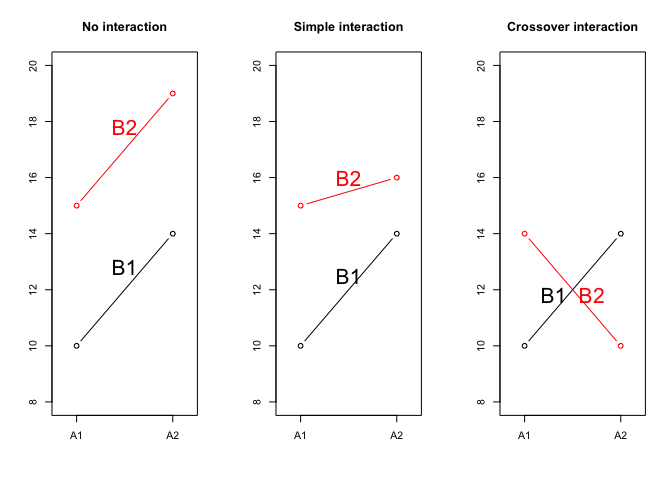
\includegraphics{_main_files/figure-latex/unnamed-chunk-105-1.pdf}

L'entità e il tipo di interazione tra fattori sperimentali possono
essere studiati solo con esperimenti combinati a più fattori
(esperimenti fattoriali) e mai con esperimenti singoli.

\section{Descrizione del caso studio}\label{descrizione-del-caso-studio}

Un ricercatore ha organizzato un esperimento fattoriale a blocchi
randomizzati, dove ha valutato l'effetto di tre tipi di lavorazione del
terreno (lavorazione minima = MIN; aratura superficiale = SUP; aratura
profonda = PROF) e di due tipi di diserbo chimico (a pieno campo = TOT;
localizzato sulla fila della coltura = PARZ). L'ipotesi scientifica è
che, in caso di diserbo localizzato, il rovesciamento del terreno
prodotto dall'aratura sia fondamentale, in quanto sotterra i semi
prodotti dalle piante infestanti, impedendone l'emergenza nella coltura
successiva e rendendo quindi necessario il diserbo a tutta superficie.
La mappa di campo è esemplificata nel disegno seguente, dove i colori
contraddistinguono i quattro blocchi.

\begin{figure}
\centering
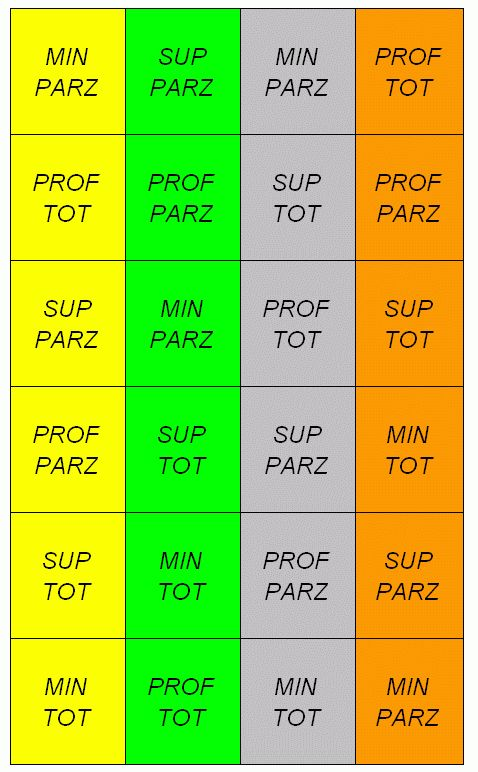
\includegraphics[width=0.45000\textwidth]{_images/SchemaFattorialeBlocchi.jpg}
\caption{}
\end{figure}

In totale, l'esperimento include sei tesi (le sei possibili combinazioni
tra i due fattori sperimentali) e quattro repliche per un totale di 24
parcelle. Come consuetudine in pieno campo, l'esperimento è organizzato
a blocchi randomizzati e le sei tesi sperimentali sono allocate a caso
all'interno di ciascun blocco.

I risultati ottenuti con questo esperimento sono disponibili nel file
`beet.csv', che può essere aperto direttamente da gitHub, con il codice
sottostante.

\begin{Shaded}
\begin{Highlighting}[]
\NormalTok{dataset <-}\StringTok{ }\KeywordTok{read.csv}\NormalTok{(}\StringTok{"https://raw.githubusercontent.com/OnofriAndreaPG/aomisc/master/data/beet.csv"}\NormalTok{, }\DataTypeTok{header=}\NormalTok{T)}
\KeywordTok{head}\NormalTok{(dataset)}
\NormalTok{##   Lavorazione Diserbo Blocco   Prod}
\NormalTok{## 1         MIN     tot      1 11.614}
\NormalTok{## 2         MIN     tot      2  9.283}
\NormalTok{## 3         MIN     tot      3  7.019}
\NormalTok{## 4         MIN     tot      4  8.015}
\NormalTok{## 5         MIN    parz      1  5.117}
\NormalTok{## 6         MIN    parz      2  4.306}
\end{Highlighting}
\end{Shaded}

\section{Analisi dei dati}\label{analisi-dei-dati-1}

Il modello lineare è:

\[y_{i,j,k} = \mu + \gamma_k + \alpha_i + \beta_j + \alpha\beta_{i,j} + \varepsilon_{i,j,k}\]

dove \(\gamma\) è l'effetto del blocco, \(\alpha\) è l'effetto della
lavorazione, \(\beta\) è l'effetto del diserbo, \(\alpha\beta\) è la
loro interazione, mentre \(\varepsilon\) è l'errore associato ad ogni
osservazione, che si assume normalmente distribuito con media 0 e
deviazione standard pari a \(\sigma\).

Per rendere `stimabili' i parametri, poniamo un vincolo sul trattamento,
per cui \(\gamma_1 = 0\), \(\alpha_1 = 0\) (primo livello in ordine
alfabetico, cioè MIN), \(\beta_1 = 0\) (primo livello in ordine
alfabetico, cioè PARZ). Per quanto riguarda l'interazione
\(\alpha\beta\), abbiamo 6 combinazioni possibili tra il primo e il
secondo fattore (MIN - TOT, MIN - PARZ, SUP - TOT, SUP - PARZ, PROF -
TOT, PROF - PARZ); di queste, dobbiamo vincolare tutte le combinazioni
che contengono il primo livello in ordine alfabetico per uno dei due
fattori (MIN - TOT, MIN - PARZ, SUP - PARZ, PROF - PARZ, corrispondenti
ad \(\alpha\beta_{1,1}\), \(\alpha\beta_{1,2}\), \(\alpha\beta_{2,1}\)
ed \(\alpha\beta_{3,1}\) = 0). In questo modo, \(\mu\) è il valore
atteso per la parcella localizzata nel primo blocco e trattata con il
primo livello in ordine alfabetico per tutti i fattori sperimentali (MIN
- PARZ). Dobbiamo stimare un intercetta, tre valori per \(\gamma\), due
valori per \(\alpha\), un valore per\(\beta\) e due valori per
\(\alpha\beta\), per un totale di nove parametri.

\section{Stima dei parametri}\label{stima-dei-parametri-1}

Trattandosi di un modello lineare con errori gaussiani, la stima dei
parametri può essere effettuata con il metodo dei minimi quadrati, cioè
cercando i valori dei parametri che rendano minima la somma dei quadrati
dei residui. In R, utilizziamo la funzione lm(), come per tutti gli
altri modelli ANOVA.

\begin{Shaded}
\begin{Highlighting}[]
\NormalTok{mod <-}\StringTok{ }\KeywordTok{lm}\NormalTok{(Prod }\OperatorTok{~}\StringTok{ }\KeywordTok{factor}\NormalTok{(Blocco) }\OperatorTok{+}\StringTok{ }\NormalTok{Lavorazione }\OperatorTok{+}\StringTok{ }\NormalTok{Diserbo }\OperatorTok{+}
\StringTok{            }\NormalTok{Lavorazione}\OperatorTok{:}\NormalTok{Diserbo, }\DataTypeTok{data=}\NormalTok{dataset)}
\KeywordTok{summary}\NormalTok{(mod)}
\NormalTok{## }
\NormalTok{## Call:}
\NormalTok{## lm(formula = Prod ~ factor(Blocco) + Lavorazione + Diserbo + }
\NormalTok{##     Lavorazione:Diserbo, data = dataset)}
\NormalTok{## }
\NormalTok{## Residuals:}
\NormalTok{##      Min       1Q   Median       3Q      Max }
\NormalTok{## -1.78329 -0.78754 -0.04437  0.31117  3.12546 }
\NormalTok{## }
\NormalTok{## Coefficients:}
\NormalTok{##                            Estimate Std. Error t value Pr(>|t|)    }
\NormalTok{## (Intercept)                  6.6422     0.8376   7.930 9.59e-07 ***}
\NormalTok{## factor(Blocco)2             -1.0380     0.7897  -1.314 0.208431    }
\NormalTok{## factor(Blocco)3             -0.8277     0.7897  -1.048 0.311179    }
\NormalTok{## factor(Blocco)4             -0.7232     0.7897  -0.916 0.374267    }
\NormalTok{## LavorazionePROF              4.6338     0.9671   4.791 0.000238 ***}
\NormalTok{## LavorazioneSUP               2.4803     0.9671   2.565 0.021568 *  }
\NormalTok{## Diserbotot                   2.9878     0.9671   3.089 0.007480 ** }
\NormalTok{## LavorazionePROF:Diserbotot  -4.4098     1.3677  -3.224 0.005677 ** }
\NormalTok{## LavorazioneSUP:Diserbotot   -2.3218     1.3677  -1.698 0.110246    }
\NormalTok{## ---}
\NormalTok{## Signif. codes:  0 '***' 0.001 '**' 0.01 '*' 0.05 '.' 0.1 ' ' 1}
\NormalTok{## }
\NormalTok{## Residual standard error: 1.368 on 15 degrees of freedom}
\NormalTok{## Multiple R-squared:  0.641,  Adjusted R-squared:  0.4495 }
\NormalTok{## F-statistic: 3.348 on 8 and 15 DF,  p-value: 0.02095}
\end{Highlighting}
\end{Shaded}

Una volta stimati i parametri, possiamo individuare la devianza residua,
come somma dei quadrati degli scarti tra i valori attesi e i valori
osservati. I residui, in R, possono essere ottenuti con la funzione
`residuals()'.

\begin{Shaded}
\begin{Highlighting}[]
\NormalTok{RSS <-}\StringTok{ }\KeywordTok{sum}\NormalTok{( }\KeywordTok{residuals}\NormalTok{(mod)}\OperatorTok{^}\DecValTok{2}\NormalTok{ )}
\NormalTok{RSS}
\NormalTok{## [1] 28.06087}
\end{Highlighting}
\end{Shaded}

Consideriamo che la devianza del residuo ha un numero di gradi di
libertà pari alla differenza tra il numero dei dati è il numero dei
parametri stimati (24 - 9 = 15). Di conseguenza, possiamo stimare
\(\sigma\), come:

\begin{Shaded}
\begin{Highlighting}[]
\KeywordTok{sqrt}\NormalTok{(RSS}\OperatorTok{/}\DecValTok{15}\NormalTok{)}
\NormalTok{## [1] 1.367744}
\end{Highlighting}
\end{Shaded}

o, più velocemente, con l'apposito estrattore:

\begin{Shaded}
\begin{Highlighting}[]
\KeywordTok{summary}\NormalTok{(mod)}\OperatorTok{$}\NormalTok{sigma}
\NormalTok{## [1] 1.367744}
\end{Highlighting}
\end{Shaded}

\section{Verifica delle assunzioni di
base}\label{verifica-delle-assunzioni-di-base}

A questo punto dobbiamo procedere con la verifica delle assunzioni di
base, plottando, come usuale, i residui contro i valori attesi.

\begin{Shaded}
\begin{Highlighting}[]
\KeywordTok{par}\NormalTok{(}\DataTypeTok{mfrow=}\KeywordTok{c}\NormalTok{(}\DecValTok{1}\NormalTok{,}\DecValTok{2}\NormalTok{))}
\KeywordTok{plot}\NormalTok{(mod, }\DataTypeTok{which =} \DecValTok{1}\NormalTok{)}
\KeywordTok{plot}\NormalTok{(mod, }\DataTypeTok{which =} \DecValTok{2}\NormalTok{)}
\end{Highlighting}
\end{Shaded}

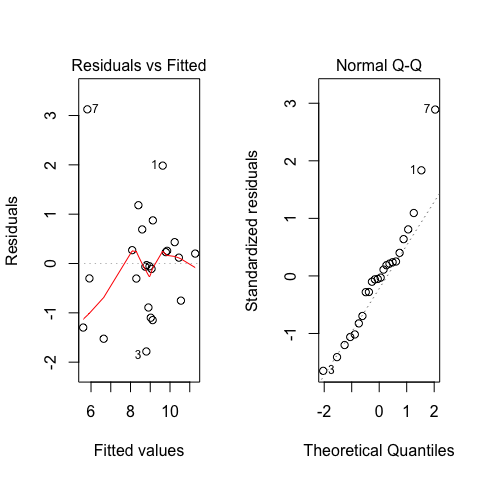
\includegraphics{_main_files/figure-latex/unnamed-chunk-111-1.pdf}

Il grafico dei residui mostra un sospetto outlier (il settimo dato).
Tuttavia, non abbiamo memoria di errori durante la sperimentazione e non
paiono esserci problemi di omogeneità delle varianze.

La procedura indicata da Box e Cox, non rivela la necessità di
trasformazioni, in quanto gli intervalli di confidenza di \(\lambda\)
contengono il valore 1.

\begin{Shaded}
\begin{Highlighting}[]
\KeywordTok{library}\NormalTok{(MASS)}
\KeywordTok{par}\NormalTok{(}\DataTypeTok{mfrow=}\KeywordTok{c}\NormalTok{(}\DecValTok{1}\NormalTok{,}\DecValTok{1}\NormalTok{))}
\KeywordTok{boxcox}\NormalTok{(mod)}
\end{Highlighting}
\end{Shaded}

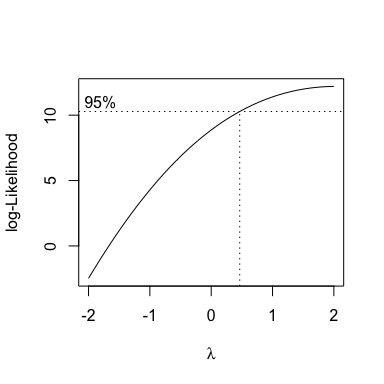
\includegraphics{_main_files/figure-latex/unnamed-chunk-112-1.pdf}

Decidiamo quindi di ignorare il sospetto dato aberrante e proseguire
nell'analisi, in quanto non sussistono particolare elementi che facciano
sospettare qualche patologia dei dati più o meno rilevante.

\section{Scomposizione delle
varianze}\label{scomposizione-delle-varianze}

Se dovessimo scomporre le varianze manualmente, potremmo costruire il
modello in modo incrementale, il che è totalmente corretto con i disegni
bilanciati come il nostro.

\begin{Shaded}
\begin{Highlighting}[]
\NormalTok{mod0 <-}\StringTok{ }\KeywordTok{lm}\NormalTok{(Prod }\OperatorTok{~}\StringTok{ }\DecValTok{1}\NormalTok{, }\DataTypeTok{data=}\NormalTok{dataset)}
\NormalTok{mod1 <-}\StringTok{ }\KeywordTok{lm}\NormalTok{(Prod }\OperatorTok{~}\StringTok{ }\KeywordTok{factor}\NormalTok{(Blocco), }\DataTypeTok{data=}\NormalTok{dataset)}
\NormalTok{mod2 <-}\StringTok{ }\KeywordTok{lm}\NormalTok{(Prod }\OperatorTok{~}\StringTok{ }\KeywordTok{factor}\NormalTok{(Blocco) }\OperatorTok{+}\StringTok{ }\NormalTok{Lavorazione, }\DataTypeTok{data=}\NormalTok{dataset)}
\NormalTok{mod3 <-}\StringTok{ }\KeywordTok{lm}\NormalTok{(Prod }\OperatorTok{~}\StringTok{ }\KeywordTok{factor}\NormalTok{(Blocco) }\OperatorTok{+}\StringTok{ }\NormalTok{Lavorazione }\OperatorTok{+}\StringTok{ }\NormalTok{Diserbo, }\DataTypeTok{data=}\NormalTok{dataset)}
\NormalTok{mod4 <-}\StringTok{ }\KeywordTok{lm}\NormalTok{(Prod }\OperatorTok{~}\StringTok{ }\KeywordTok{factor}\NormalTok{(Blocco) }\OperatorTok{+}\StringTok{ }\NormalTok{Lavorazione }\OperatorTok{+}\StringTok{ }\NormalTok{Diserbo }\OperatorTok{+}
\StringTok{            }\NormalTok{Lavorazione}\OperatorTok{:}\NormalTok{Diserbo, }\DataTypeTok{data=}\NormalTok{dataset)}
\NormalTok{RSS0 <-}\StringTok{ }\KeywordTok{deviance}\NormalTok{(mod0)}
\NormalTok{RSS1 <-}\StringTok{ }\KeywordTok{deviance}\NormalTok{(mod1)}
\NormalTok{RSS2 <-}\StringTok{ }\KeywordTok{deviance}\NormalTok{(mod2)}
\NormalTok{RSS3 <-}\StringTok{ }\KeywordTok{deviance}\NormalTok{(mod3)}
\NormalTok{RSS4 <-}\StringTok{ }\KeywordTok{deviance}\NormalTok{(mod4)}
\end{Highlighting}
\end{Shaded}

Vediamo che il modello nullo ha un residuo pari a 78.161505, mentre il
il modello con il solo effetto del blocco ha un residuo più basso e pari
74.5019152. Evidentemente, l'introduzione del blocco ha migliorato la
capacità descrittiva del modello e l'effetto di questa variabile può
essere quantificato con la differenza tra le due devianze:

\begin{Shaded}
\begin{Highlighting}[]
\NormalTok{RSS0 }\OperatorTok{-}\StringTok{ }\NormalTok{RSS1}
\NormalTok{## [1] 3.65959}
\end{Highlighting}
\end{Shaded}

Analogamente, l'effetto della lavorazione (devianza della lavorazione) è
dato da:

\begin{Shaded}
\begin{Highlighting}[]
\NormalTok{RSS1 }\OperatorTok{-}\StringTok{ }\NormalTok{RSS2}
\NormalTok{## [1] 23.65647}
\end{Highlighting}
\end{Shaded}

Ovviamente, possiamo evitare di procedere in questo modo, sfruttando le
funzionalità di R e, in particolare, la funzione `anova()':

\begin{Shaded}
\begin{Highlighting}[]
\KeywordTok{anova}\NormalTok{(mod)}
\NormalTok{## Analysis of Variance Table}
\NormalTok{## }
\NormalTok{## Response: Prod}
\NormalTok{##                     Df  Sum Sq Mean Sq F value  Pr(>F)  }
\NormalTok{## factor(Blocco)       3  3.6596  1.2199  0.6521 0.59389  }
\NormalTok{## Lavorazione          2 23.6565 11.8282  6.3228 0.01020 *}
\NormalTok{## Diserbo              1  3.3205  3.3205  1.7750 0.20266  }
\NormalTok{## Lavorazione:Diserbo  2 19.4641  9.7321  5.2023 0.01922 *}
\NormalTok{## Residuals           15 28.0609  1.8707                  }
\NormalTok{## ---}
\NormalTok{## Signif. codes:  0 '***' 0.001 '**' 0.01 '*' 0.05 '.' 0.1 ' ' 1}
\end{Highlighting}
\end{Shaded}

La quantificazione dei gradi di libertà dovrebbe essere chiara;
aggiungiamo solo che, in generale, i gradi di libertà di un'interazione
sono pari al prodotto tra i gradi di libertà degli effetti da cui essa è
composta e coincidono con il numero di parametri stimati (in questo caso
due).

Nel leggere una tabella ANOVA a due (o più) vie, è \textbf{fondamentale
procedere dal basso verso l'alto}, in quanto la presenza di
un'interazione significativa rende non-informative sia le significanze
degli effetti principali, sia le medie marginali. Infatti, come abbiamo
visto all'inizio, vi possono essere casi in cui le medie marginali sono
simili, ma ciò è dovuto alla presenza di un'interazione CROSSOVER. In
questo caso, essendo significativa l'interazione tra lavorazione e
diserbo, dovremo considerare e confrontare le sei medie per le
combinazioni tra questi due fattori sperimentali.

\section{Funzioni dei parametri}\label{funzioni-dei-parametri}

\subsection{\texorpdfstring{Medie delle combinazioni `lavorazioni x
diserbo'}{Medie delle combinazioni lavorazioni x diserbo}}\label{medie-delle-combinazioni-lavorazioni-x-diserbo}

Le medie attese per le sei combinazioni `lavorazione x diserbo' possono
essere ottenute attraverso apposite combinazioni (funzioni) dei
parametri stimati. Ad esempio, sappiamo che \(\mu\) è il valore atteso
per MIN-PARZ nel primo blocco, mentre \(\mu + \gamma_2\) è il valore
atteso per MIN-PARZ nel secondo blocco, e così via. Di conseguenza, la
media per la combinazione MIN-PARZ sarà pari a:

\[ \frac{\mu + (\mu + \gamma_2) + (\mu + \gamma_3) + (\mu + \gamma_4)}{4} = \mu + \frac{1}{4}\gamma_2 + \frac{1}{4}\gamma_3 + \frac{1}{4}\gamma_4\]

I parametri stimati sono derivabili con la funzione `coef()', quindi la
combinazione lineare sopra indicata può essere ottenuta come segue:

\begin{Shaded}
\begin{Highlighting}[]
\KeywordTok{coef}\NormalTok{(mod)[}\DecValTok{1}\NormalTok{] }\OperatorTok{+}\StringTok{ }\DecValTok{1}\OperatorTok{/}\DecValTok{4}\OperatorTok{*}\KeywordTok{coef}\NormalTok{(mod)[}\DecValTok{2}\NormalTok{] }\OperatorTok{+}\StringTok{ }\DecValTok{1}\OperatorTok{/}\DecValTok{4}\OperatorTok{*}\KeywordTok{coef}\NormalTok{(mod)[}\DecValTok{3}\NormalTok{] }\OperatorTok{+}\StringTok{ }\DecValTok{1}\OperatorTok{/}\DecValTok{4}\OperatorTok{*}\KeywordTok{coef}\NormalTok{(mod)[}\DecValTok{4}\NormalTok{]}
\NormalTok{## (Intercept) }
\NormalTok{##       5.995}
\end{Highlighting}
\end{Shaded}

Ovviamente, è più conveniente costruire una vettore con i coefficienti
del contrasto, e moltiplicare per il vettore dei parametri stimati, come
segue:

\begin{Shaded}
\begin{Highlighting}[]
\NormalTok{k1 <-}\StringTok{ }\KeywordTok{c}\NormalTok{(}\DecValTok{1}\NormalTok{, }\DecValTok{1}\OperatorTok{/}\DecValTok{4}\NormalTok{, }\DecValTok{1}\OperatorTok{/}\DecValTok{4}\NormalTok{, }\DecValTok{1}\OperatorTok{/}\DecValTok{4}\NormalTok{, }\DecValTok{0}\NormalTok{, }\DecValTok{0}\NormalTok{, }\DecValTok{0}\NormalTok{, }\DecValTok{0}\NormalTok{, }\DecValTok{0}\NormalTok{)}
\KeywordTok{sum}\NormalTok{( }\KeywordTok{coef}\NormalTok{(mod) }\OperatorTok{*}\StringTok{ }\NormalTok{k1 )}
\NormalTok{## [1] 5.995}
\end{Highlighting}
\end{Shaded}

Le altre medie, possono essere ottenute analogamente.

\begin{Shaded}
\begin{Highlighting}[]
\NormalTok{k2 <-}\StringTok{ }\KeywordTok{c}\NormalTok{(}\DecValTok{1}\NormalTok{, }\DecValTok{1}\OperatorTok{/}\DecValTok{4}\NormalTok{, }\DecValTok{1}\OperatorTok{/}\DecValTok{4}\NormalTok{, }\DecValTok{1}\OperatorTok{/}\DecValTok{4}\NormalTok{, }\DecValTok{1}\NormalTok{, }\DecValTok{0}\NormalTok{, }\DecValTok{0}\NormalTok{, }\DecValTok{0}\NormalTok{, }\DecValTok{0}\NormalTok{) }\CommentTok{#PROF - PARZ}
\NormalTok{k3 <-}\StringTok{ }\KeywordTok{c}\NormalTok{(}\DecValTok{1}\NormalTok{, }\DecValTok{1}\OperatorTok{/}\DecValTok{4}\NormalTok{, }\DecValTok{1}\OperatorTok{/}\DecValTok{4}\NormalTok{, }\DecValTok{1}\OperatorTok{/}\DecValTok{4}\NormalTok{, }\DecValTok{0}\NormalTok{, }\DecValTok{1}\NormalTok{, }\DecValTok{0}\NormalTok{, }\DecValTok{0}\NormalTok{, }\DecValTok{0}\NormalTok{) }\CommentTok{#SUP - PARZ}
\NormalTok{k4 <-}\StringTok{ }\KeywordTok{c}\NormalTok{(}\DecValTok{1}\NormalTok{, }\DecValTok{1}\OperatorTok{/}\DecValTok{4}\NormalTok{, }\DecValTok{1}\OperatorTok{/}\DecValTok{4}\NormalTok{, }\DecValTok{1}\OperatorTok{/}\DecValTok{4}\NormalTok{, }\DecValTok{0}\NormalTok{, }\DecValTok{0}\NormalTok{, }\DecValTok{1}\NormalTok{, }\DecValTok{0}\NormalTok{, }\DecValTok{0}\NormalTok{) }\CommentTok{#MIN - TOT}
\NormalTok{k5 <-}\StringTok{ }\KeywordTok{c}\NormalTok{(}\DecValTok{1}\NormalTok{, }\DecValTok{1}\OperatorTok{/}\DecValTok{4}\NormalTok{, }\DecValTok{1}\OperatorTok{/}\DecValTok{4}\NormalTok{, }\DecValTok{1}\OperatorTok{/}\DecValTok{4}\NormalTok{, }\DecValTok{1}\NormalTok{, }\DecValTok{0}\NormalTok{, }\DecValTok{1}\NormalTok{, }\DecValTok{1}\NormalTok{, }\DecValTok{0}\NormalTok{) }\CommentTok{#PROF - TOT}
\NormalTok{k6 <-}\StringTok{ }\KeywordTok{c}\NormalTok{(}\DecValTok{1}\NormalTok{, }\DecValTok{1}\OperatorTok{/}\DecValTok{4}\NormalTok{, }\DecValTok{1}\OperatorTok{/}\DecValTok{4}\NormalTok{, }\DecValTok{1}\OperatorTok{/}\DecValTok{4}\NormalTok{, }\DecValTok{0}\NormalTok{, }\DecValTok{1}\NormalTok{, }\DecValTok{1}\NormalTok{, }\DecValTok{0}\NormalTok{, }\DecValTok{1}\NormalTok{) }\CommentTok{#SUP - TOT}
\KeywordTok{sum}\NormalTok{( }\KeywordTok{coef}\NormalTok{(mod) }\OperatorTok{*}\StringTok{ }\NormalTok{k2 )}
\NormalTok{## [1] 10.62875}
\KeywordTok{sum}\NormalTok{( }\KeywordTok{coef}\NormalTok{(mod) }\OperatorTok{*}\StringTok{ }\NormalTok{k3 )}
\NormalTok{## [1] 8.47525}
\KeywordTok{sum}\NormalTok{( }\KeywordTok{coef}\NormalTok{(mod) }\OperatorTok{*}\StringTok{ }\NormalTok{k4 )}
\NormalTok{## [1] 8.98275}
\KeywordTok{sum}\NormalTok{( }\KeywordTok{coef}\NormalTok{(mod) }\OperatorTok{*}\StringTok{ }\NormalTok{k5 )}
\NormalTok{## [1] 9.20675}
\KeywordTok{sum}\NormalTok{( }\KeywordTok{coef}\NormalTok{(mod) }\OperatorTok{*}\StringTok{ }\NormalTok{k6 )}
\NormalTok{## [1] 9.14125}
\end{Highlighting}
\end{Shaded}

\section{Calcolo degli errori standard (SEM e
SED)}\label{calcolo-degli-errori-standard-sem-e-sed}

Tutte le quantità ottenute più sopra sono state calcolate come
combinazioni lineari di parametri del modello. Di conseguenza, le loro
varianze sono derivabili con la legge di propagazione degli errori. In
questo caso semplice (dati bilanciati), possiamo utilizzare la usuale
formula per la quale l'errore standard di una media si ottiene dalla
radice quadrata del rapporto tra la varianza del residuo e il numero
delle repliche. Tuttavia, anche se la varianza del residuo è la stessa,
il numero di dati che concorrono a formare le medie è diverso (diverso
numero di repliche). Infatti, le medie di ogni combinazione `diserbo x
lavorazione' hanno un numero di repliche pari a quattro, mentre le
lavorazioni hanno un numero di repliche pari a quattro per il numero dei
livelli di diserbo (cioè 8). Il diserbo ha invece un numero di repliche
pari a quattro per il numero dei livelli di lavorazione (cioè 12).

Di conseguenza:

\[SEM_A = \sqrt{\frac{1.87}{4 \cdot 2}} = 0.483\]

\[SEM_B = \sqrt{\frac{1.87}{4 \cdot 3}} = 0.395\]

\[SEM_{AB} = \sqrt{\frac{1.87}{4}} = 0.684\]

Possiamo notare che le medie degli effetti principali, grazie al numero
di repliche più elevato, sono stimate con maggiore precisione delle
medie delle combinazioni.

Per quanto riguarda gli errori standard delle differenze tra medie
(SED), questi si ottengono dai SEM, moltiplicandoli per \(\sqrt(2)\),
come usuale. Dai SED, posso calcolare le Minime Differenze
Significative, moltiplicandoli per il valore di t di Student, per il 5\%
di probabilità (test a due code) e 15 gradi di libertà, pari a 2.131.

Dato che l'interazione è significativa, posso fare i confronti multipli
solo tra le medie delle combinazioni `diserbo x lavorazione', dato che
confrontare le medie degli effetti principali potrebbe portare a
risultati poco attendibili, per i motivi precedentemente esposti.

\section{Contrasti, medie attese e confronti multipli con
R}\label{contrasti-medie-attese-e-confronti-multipli-con-r}

Lavorare con i contrasti è molto utile, perché, con un'accurata
selezione dei coefficienti, possiamo facilmente definire ogni tipo di di
ipotesi biologica, da sottoporre a test statistico. Per questo, possiamo
utilizzare il package `multcomp' e la funzione `glht()'.

In primo luogo, dobbiamo definire una matrice dei contrasti, che ospita
i vettori dei coefficienti. Per le sei medie sopra determinate, questa
matrice è:

\begin{Shaded}
\begin{Highlighting}[]
\NormalTok{M <-}\StringTok{ }\KeywordTok{matrix}\NormalTok{(}\KeywordTok{c}\NormalTok{(k1, k2, k3, k4, k5, k6), }\DecValTok{6}\NormalTok{, }\DecValTok{9}\NormalTok{, }\DataTypeTok{byrow =}\NormalTok{ T)}
\NormalTok{M}
\NormalTok{##      [,1] [,2] [,3] [,4] [,5] [,6] [,7] [,8] [,9]}
\NormalTok{## [1,]    1 0.25 0.25 0.25    0    0    0    0    0}
\NormalTok{## [2,]    1 0.25 0.25 0.25    1    0    0    0    0}
\NormalTok{## [3,]    1 0.25 0.25 0.25    0    1    0    0    0}
\NormalTok{## [4,]    1 0.25 0.25 0.25    0    0    1    0    0}
\NormalTok{## [5,]    1 0.25 0.25 0.25    1    0    1    1    0}
\NormalTok{## [6,]    1 0.25 0.25 0.25    0    1    1    0    1}
\end{Highlighting}
\end{Shaded}

Dopo aver definito la matrice, possiamo utilizzarla come argomento della
funzione `glht()', in questo modo

\begin{Shaded}
\begin{Highlighting}[]
\KeywordTok{library}\NormalTok{(multcomp)}
\NormalTok{mc <-}\StringTok{ }\KeywordTok{glht}\NormalTok{(mod, }\DataTypeTok{linfct =}\NormalTok{ M)}
\KeywordTok{summary}\NormalTok{(mc, }\DataTypeTok{test=}\KeywordTok{adjusted}\NormalTok{(}\DataTypeTok{type=}\StringTok{"none"}\NormalTok{))}
\NormalTok{## }
\NormalTok{##   Simultaneous Tests for General Linear Hypotheses}
\NormalTok{## }
\NormalTok{## Fit: lm(formula = Prod ~ factor(Blocco) + Lavorazione + Diserbo + }
\NormalTok{##     Lavorazione:Diserbo, data = dataset)}
\NormalTok{## }
\NormalTok{## Linear Hypotheses:}
\NormalTok{##        Estimate Std. Error t value Pr(>|t|)    }
\NormalTok{## 1 == 0   5.9950     0.6839   8.766 2.74e-07 ***}
\NormalTok{## 2 == 0  10.6288     0.6839  15.542 1.17e-10 ***}
\NormalTok{## 3 == 0   8.4753     0.6839  12.393 2.78e-09 ***}
\NormalTok{## 4 == 0   8.9828     0.6839  13.135 1.25e-09 ***}
\NormalTok{## 5 == 0   9.2068     0.6839  13.463 8.84e-10 ***}
\NormalTok{## 6 == 0   9.1413     0.6839  13.367 9.77e-10 ***}
\NormalTok{## ---}
\NormalTok{## Signif. codes:  0 '***' 0.001 '**' 0.01 '*' 0.05 '.' 0.1 ' ' 1}
\NormalTok{## (Adjusted p values reported -- none method)}
\end{Highlighting}
\end{Shaded}

Questo approccio è molto utile per un `fine tuning' ottimale dei
contrasti. In generale, per ottenere medie, confronti multipli o altre
analisi routinarie, possiamo utilizzare il package `emmeans'. Il codice
sottostante calcola le medie per le combinazioni `lavorazione x diserbo'
e confronta i diserbi a parità di lavorazione.

\begin{Shaded}
\begin{Highlighting}[]
\KeywordTok{library}\NormalTok{(emmeans)}
\NormalTok{medie <-}\StringTok{ }\KeywordTok{emmeans}\NormalTok{(mod, }\OperatorTok{~}\NormalTok{Diserbo}\OperatorTok{|}\NormalTok{Lavorazione)}
\KeywordTok{cld}\NormalTok{(medie, }\DataTypeTok{adjust=}\StringTok{"none"}\NormalTok{, }\DataTypeTok{Letters=}\NormalTok{LETTERS)}
\NormalTok{## Lavorazione = MIN:}
\NormalTok{##  Diserbo   emmean        SE df lower.CL  upper.CL .group}
\NormalTok{##  parz     5.99500 0.6838722 15 4.537361  7.452639  A    }
\NormalTok{##  tot      8.98275 0.6838722 15 7.525111 10.440389   B   }
\NormalTok{## }
\NormalTok{## Lavorazione = PROF:}
\NormalTok{##  Diserbo   emmean        SE df lower.CL  upper.CL .group}
\NormalTok{##  tot      9.20675 0.6838722 15 7.749111 10.664389  A    }
\NormalTok{##  parz    10.62875 0.6838722 15 9.171111 12.086389  A    }
\NormalTok{## }
\NormalTok{## Lavorazione = SUP:}
\NormalTok{##  Diserbo   emmean        SE df lower.CL  upper.CL .group}
\NormalTok{##  parz     8.47525 0.6838722 15 7.017611  9.932889  A    }
\NormalTok{##  tot      9.14125 0.6838722 15 7.683611 10.598889  A    }
\NormalTok{## }
\NormalTok{## Results are averaged over the levels of: Blocco }
\NormalTok{## Confidence level used: 0.95 }
\NormalTok{## significance level used: alpha = 0.05}
\end{Highlighting}
\end{Shaded}

Se volessimo confrontare le lavorazioni a parità di diserbo o tutte le
combinazioni dovremmo utilizzare codice leggermente diverso:

\begin{Shaded}
\begin{Highlighting}[]
\NormalTok{medie <-}\StringTok{ }\KeywordTok{emmeans}\NormalTok{(mod, }\OperatorTok{~}\NormalTok{Lavorazione}\OperatorTok{|}\NormalTok{Diserbo)}
\KeywordTok{cld}\NormalTok{(medie, }\DataTypeTok{adjust=}\StringTok{"none"}\NormalTok{, }\DataTypeTok{Letters=}\NormalTok{LETTERS)}
\NormalTok{## Diserbo = parz:}
\NormalTok{##  Lavorazione   emmean        SE df lower.CL  upper.CL .group}
\NormalTok{##  MIN          5.99500 0.6838722 15 4.537361  7.452639  A    }
\NormalTok{##  SUP          8.47525 0.6838722 15 7.017611  9.932889   B   }
\NormalTok{##  PROF        10.62875 0.6838722 15 9.171111 12.086389    C  }
\NormalTok{## }
\NormalTok{## Diserbo = tot:}
\NormalTok{##  Lavorazione   emmean        SE df lower.CL  upper.CL .group}
\NormalTok{##  MIN          8.98275 0.6838722 15 7.525111 10.440389  A    }
\NormalTok{##  SUP          9.14125 0.6838722 15 7.683611 10.598889  A    }
\NormalTok{##  PROF         9.20675 0.6838722 15 7.749111 10.664389  A    }
\NormalTok{## }
\NormalTok{## Results are averaged over the levels of: Blocco }
\NormalTok{## Confidence level used: 0.95 }
\NormalTok{## significance level used: alpha = 0.05}
\NormalTok{medie <-}\StringTok{ }\KeywordTok{emmeans}\NormalTok{(mod, }\OperatorTok{~}\NormalTok{Lavorazione}\OperatorTok{:}\NormalTok{Diserbo)}
\KeywordTok{cld}\NormalTok{(medie, }\DataTypeTok{adjust=}\StringTok{"none"}\NormalTok{, }\DataTypeTok{Letters=}\NormalTok{LETTERS)}
\NormalTok{##  Lavorazione Diserbo   emmean        SE df lower.CL  upper.CL .group}
\NormalTok{##  MIN         parz     5.99500 0.6838722 15 4.537361  7.452639  A    }
\NormalTok{##  SUP         parz     8.47525 0.6838722 15 7.017611  9.932889   B   }
\NormalTok{##  MIN         tot      8.98275 0.6838722 15 7.525111 10.440389   BC  }
\NormalTok{##  SUP         tot      9.14125 0.6838722 15 7.683611 10.598889   BC  }
\NormalTok{##  PROF        tot      9.20675 0.6838722 15 7.749111 10.664389   BC  }
\NormalTok{##  PROF        parz    10.62875 0.6838722 15 9.171111 12.086389    C  }
\NormalTok{## }
\NormalTok{## Results are averaged over the levels of: Blocco }
\NormalTok{## Confidence level used: 0.95 }
\NormalTok{## significance level used: alpha = 0.05}
\end{Highlighting}
\end{Shaded}

In questo caso non c'è nessuna differenza, dato che non abbiamo
implementato nessuna correzione per la molteplicità. Altrimenti, le tre
situazioni sarebbero diverse, in quanto nel primo caso avremmo fatto
solo tre confronti, nel secondo caso ne avremmo fatti sei, nel terzo
caso 15, con un diverso livello di correzione per la molteplicità.

\chapter{La regressione lineare
semplice}\label{la-regressione-lineare-semplice}

\section{Introduzione}\label{introduzione-5}

Nella sperimentazione agronomica e biologica in genere è normale
organizzare prove sperimentali replicate, anche per studiare l'effetto
di una fattore quantitativo su una variabile dipendente, anch'essa
quantitativa.

In questa situazione, l'impiego di metodiche di confronto multiplo, se
non del tutto errato, è comunque da considerare `improprio'. Infatti,
l'inclusione di alcuni particolari livelli della variabile indipendente
è frutto solo delle esigenze organizzative, senza alcune interesse
particolare per lo sperimentatore, che è invece interessato a capire
come cresce/decresce/varia la Y (variabile dipendente) in funzione della
X (variabile indipendente). In sostanza lo sperimentatore è interessato
a definire una funzione di risposta per tutto il range delle X, non a
confrontare le risposte a due particolari livelli di X.

\section{Esempio}\label{esempio-6}

Per meglio comprendere la componente stocastica degli esperimenti,
immaginiamo di conoscere la legge deterministica che definisce la
risposta del frumento alla concimazione azotata. In particolare,
immaginiamo che questa risposta produttiva sia fondamentalmente lineare:

\[Y_E = b_0 + b_1 X\]

ed immaginiamo che, senza concimazione (X = 0), la produzione sia pari a
25 q/ha (\(b_0\) = 25). Immaginiamo che l'incremente produttivo per kg
di azoto somministrato sia pari a 0.15 q/ha (\(b_1\) = 0.15).

Per individuare questa legge naturale organizziamo un esperimento, con
quattro dosi di azoto e quattro repliche. In questo esperimento, come in
tutti gli esperimenti, agirà anche una componente stocastica, che in
qualche modo sposterà la risposta osservata dalla risposta attesa:

\[Y_o = b_0 + b_1 X + \varepsilon \quad \textrm{con}  \quad \varepsilon \sim N(0, \sigma)\]

Si assume che la componente stocastica \(\varepsilon\) sia distribuita
normalmente, come media 0 e deviazione standard \(\sigma\), che
immaginiamo essere pari a 2.5 q/ha.

Su questa base, generiamo i dati osservati.

\begin{Shaded}
\begin{Highlighting}[]
\KeywordTok{set.seed}\NormalTok{(}\DecValTok{1234}\NormalTok{)}
\NormalTok{Dose <-}\StringTok{ }\KeywordTok{rep}\NormalTok{(}\KeywordTok{c}\NormalTok{(}\DecValTok{0}\NormalTok{, }\DecValTok{60}\NormalTok{, }\DecValTok{120}\NormalTok{, }\DecValTok{180}\NormalTok{), }\DataTypeTok{each=}\DecValTok{4}\NormalTok{) }
\NormalTok{Yield_E <-}\StringTok{ }\DecValTok{25} \OperatorTok{+}\StringTok{ }\FloatTok{0.15} \OperatorTok{*}\StringTok{ }\NormalTok{Dose}
\NormalTok{epsilon <-}\StringTok{ }\KeywordTok{rnorm}\NormalTok{(}\DecValTok{16}\NormalTok{, }\DecValTok{0}\NormalTok{, }\FloatTok{2.5}\NormalTok{)}
\NormalTok{Yield <-}\StringTok{ }\NormalTok{Yield_E }\OperatorTok{+}\StringTok{ }\NormalTok{epsilon}
\end{Highlighting}
\end{Shaded}

A questo punto scordiamoci la verità `vera', che non è normalmente nota,
e iniziamo l'analisi dei risultati dell'esperimento. Trattandosi di una
prova replicata, si inizia, come al solito, con l'ANOVA, che porta al
seguente risultato:

\begin{Shaded}
\begin{Highlighting}[]
\NormalTok{model <-}\StringTok{ }\KeywordTok{lm}\NormalTok{(Yield }\OperatorTok{~}\StringTok{ }\KeywordTok{factor}\NormalTok{(Dose))}
\KeywordTok{anova}\NormalTok{(model)}
\NormalTok{## Analysis of Variance Table}
\NormalTok{## }
\NormalTok{## Response: Yield}
\NormalTok{##              Df  Sum Sq Mean Sq F value    Pr(>F)    }
\NormalTok{## factor(Dose)  3 2077.43  692.48  151.77 8.315e-10 ***}
\NormalTok{## Residuals    12   54.75    4.56                      }
\NormalTok{## ---}
\NormalTok{## Signif. codes:  0 '***' 0.001 '**' 0.01 '*' 0.05 '.' 0.1 ' ' 1}
\end{Highlighting}
\end{Shaded}

Osserviamo che l'effetto del trattamento è significativo e il SEM è pari
a \(\sqrt{5.10/4} = 1.129\). Prima di proseguire, verifichiamo che non
ci siano problemi relativi alle assunzioni parametriche di base e che,
quindi, la trasformazione dei dati non sia necessaria. Il grafico dei
residui, riportato di seguito, mostra che non vi sono patologie
rilevanti.

\begin{Shaded}
\begin{Highlighting}[]
\KeywordTok{par}\NormalTok{(}\DataTypeTok{mfrow=}\KeywordTok{c}\NormalTok{(}\DecValTok{2}\NormalTok{,}\DecValTok{2}\NormalTok{))}
\KeywordTok{plot}\NormalTok{(model)}
\end{Highlighting}
\end{Shaded}

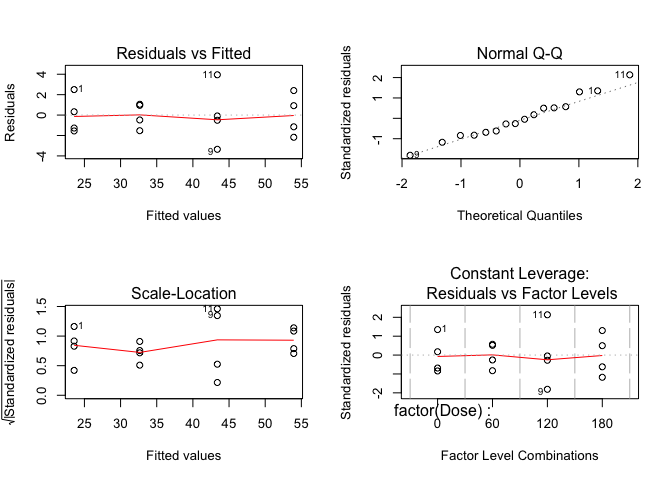
\includegraphics{_main_files/figure-latex/unnamed-chunk-126-1.pdf}

Per maggior sicurezza, possiamo anche eseguire test statistici di
verifica dell'omogeneità delle varianze (test di Bartlett e test di
Levene) o della normalità dei residui (test di Shapiro-Wilks)

\begin{Shaded}
\begin{Highlighting}[]
\KeywordTok{bartlett.test}\NormalTok{(Yield }\OperatorTok{~}\StringTok{ }\KeywordTok{factor}\NormalTok{(Dose))}
\NormalTok{## }
\NormalTok{##  Bartlett test of homogeneity of variances}
\NormalTok{## }
\NormalTok{## data:  Yield by factor(Dose)}
\NormalTok{## Bartlett's K-squared = 2.0084, df = 3, p-value = 0.5707}
\NormalTok{car}\OperatorTok{::}\KeywordTok{leveneTest}\NormalTok{(Yield }\OperatorTok{~}\StringTok{ }\KeywordTok{factor}\NormalTok{(Dose))}
\NormalTok{## Levene's Test for Homogeneity of Variance (center = median)}
\NormalTok{##       Df F value Pr(>F)}
\NormalTok{## group  3  0.4075 0.7504}
\NormalTok{##       12}
\KeywordTok{shapiro.test}\NormalTok{(}\KeywordTok{residuals}\NormalTok{(model))}
\NormalTok{## }
\NormalTok{##  Shapiro-Wilk normality test}
\NormalTok{## }
\NormalTok{## data:  residuals(model)}
\NormalTok{## W = 0.97755, p-value = 0.9411}
\end{Highlighting}
\end{Shaded}

Ovviamente, nessuno di questi strumenti diagnostici rileva problemi con
le assunzioni di base. In questo caso è ovvio, perché abbiamo generato
noi i dati sotto queste assunzioni. Normalmente questo è invece un
passaggio fondamentale.

Da questo momento in avanti, l'analisi non prosegue con un test di
confronto multiplo (infatti quale senso avrebbe confrontare tra loro le
risposte a N0, N60, N120 e così via?), ma con una analisi di
regressione.

\section{Stima dei parametri}\label{stima-dei-parametri-2}

Dobbiamo a questo punto individuare i parametri \(b_0\) e \(b_1\) in
modo tale che la retta ottenuta sia la più vicina ai dati, cioè in modo
da minimizzare gli scostamenti tra i valori di produzione osservati e
quelli stimati dal modello (soluzione dei minimi quadrati). La funzione
dei minimi quadrati è:

\[\begin{array}{l}
Q = \sum\limits_{i = }^N {\left( {{Y_i} - \hat Y} \right)^2 = \sum\limits_{i = }^N {{{\left( {{Y_i} - {b_0} - {b_1}{X_i}} \right)}^2}}  = } \\
 = \sum\limits_{i = }^N {\left( {Y_i^2 + b_0^2 + b_1^2X_i^2 - 2{Y_i}{b_0} - 2{Y_i}{b_1}{X_i} + 2{b_0}{b_1}{X_i}} \right)}  = \\
 = \sum\limits_{i = }^N {Y_i^2 + Nb_0^2 + b_1^2\sum\limits_{i = }^N {X_i^2 - 2{b_0}\sum\limits_{i = }^N {Y_i^2 - 2{b_1}\sum\limits_{i = }^N {{X_i}{Y_i} + } } } } 2{b_0}{b_1}\sum\limits_{i = }^N {{X_i}} 
\end{array}\]

Calcolando le derivate parziali rispetto a \(b_0\) e \(b_1\) che, al
momento, sono le nostre incognite, ed eguagliandole a 0 si ottengono le
seguenti formule risolutive:

\[{b_1} = \frac{{\sum\limits_{i = 1}^N {\left[ {\left( {{X_i} - {\mu _X}} \right)\left( {{Y_i} - {\mu _Y}} \right)} \right]} }}{{\sum\limits_{i = 1}^N {{{\left( {{X_i} - {\mu _X}} \right)}^2}} }}\]

e

\[{b_0} = {\mu _Y} - {b_1}{\mu _X}\]

Invece che svolgere i calcoli a mano, possiamo eseguire il fitting ai
minimi quadrati con R.

\begin{Shaded}
\begin{Highlighting}[]
\NormalTok{modelReg <-}\StringTok{ }\KeywordTok{lm}\NormalTok{(Yield }\OperatorTok{~}\StringTok{ }\NormalTok{Dose)}
\KeywordTok{summary}\NormalTok{(modelReg)}
\NormalTok{## }
\NormalTok{## Call:}
\NormalTok{## lm(formula = Yield ~ Dose)}
\NormalTok{## }
\NormalTok{## Residuals:}
\NormalTok{##     Min      1Q  Median      3Q     Max }
\NormalTok{## -3.4535 -1.0994 -0.3983  0.8945  3.8486 }
\NormalTok{## }
\NormalTok{## Coefficients:}
\NormalTok{##              Estimate Std. Error t value Pr(>|t|)    }
\NormalTok{## (Intercept) 23.111800   0.848832   27.23 1.59e-13 ***}
\NormalTok{## Dose         0.169744   0.007562   22.45 2.24e-12 ***}
\NormalTok{## ---}
\NormalTok{## Signif. codes:  0 '***' 0.001 '**' 0.01 '*' 0.05 '.' 0.1 ' ' 1}
\NormalTok{## }
\NormalTok{## Residual standard error: 2.029 on 14 degrees of freedom}
\NormalTok{## Multiple R-squared:  0.973,  Adjusted R-squared:  0.971 }
\NormalTok{## F-statistic: 503.9 on 1 and 14 DF,  p-value: 2.237e-12}
\end{Highlighting}
\end{Shaded}

Vediamo che le stime ottenute, correlate dei loro errori standard,
corrispondono bene con la verità `vera' che avevamo costruito.

\section{Valutazione della bontà del
modello}\label{valutazione-della-bonta-del-modello}

\subsection{Valutazione grafica}\label{valutazione-grafica}

Abbiamo già valutato la validità delle assunzioni di base per i modelli
lineari, in sede di ANOVA. Ora è necessario valutare se i dati osservati
sono funzione della variabile esplicativa attraverso il modello dato più
l'eventuale errore casuale, senza nessuna componente sistematica di
mancanza d'adattamento. Questo può essere fatto, nel modo più semplice,
attraverso un grafico dei valori attesi e dei valori osservati, come
quello sottostante.

\begin{Shaded}
\begin{Highlighting}[]
\KeywordTok{plot}\NormalTok{(Yield }\OperatorTok{~}\StringTok{ }\NormalTok{Dose)}
\KeywordTok{abline}\NormalTok{(modelReg, }\DataTypeTok{lty=}\DecValTok{2}\NormalTok{)}
\end{Highlighting}
\end{Shaded}

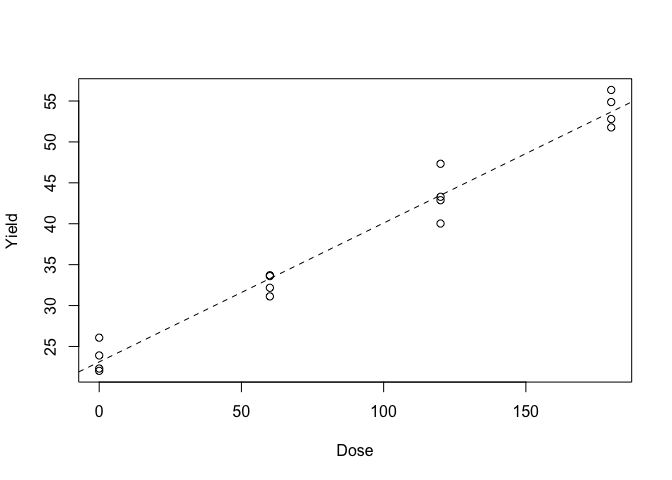
\includegraphics{_main_files/figure-latex/unnamed-chunk-129-1.pdf}

\subsection{Errori standard dei
parametri}\label{errori-standard-dei-parametri}

In secondo luogo, possiamo valutare gli errori standard delle stime dei
parametri, che non debbono mai essere superiori alla metà del valore del
parametro stimato, cosa che in questo caso è pienamente verificata. Se
così non fosse, l'intervallo di confidenza del parametro conterrebbe lo
zero, il che equivarebbe a dire che, ad esempio, la pendenza `vera'
(cioè quella della popolazione) potrebbe essere nulla. In altre parole,
la retta potrebbe quindi essere `piatta', dimostrando l'inesistenza di
relazione tra la X e la Y.

\subsection{Test F per la mancanza
d'adattamento}\label{test-f-per-la-mancanza-dadattamento}

In terzo luogo, possiamo analizzare i residui della regressione, cioè
gli scostamenti dei punti rispetto alla retta e, in particolare, la
somma dei loro quadrati. Possiamo vedere che questo valore è pari a
70.38:

\begin{Shaded}
\begin{Highlighting}[]
\KeywordTok{anova}\NormalTok{(modelReg)}
\NormalTok{## Analysis of Variance Table}
\NormalTok{## }
\NormalTok{## Response: Yield}
\NormalTok{##           Df  Sum Sq Mean Sq F value    Pr(>F)    }
\NormalTok{## Dose       1 2074.54 2074.54  503.87 2.237e-12 ***}
\NormalTok{## Residuals 14   57.64    4.12                      }
\NormalTok{## ---}
\NormalTok{## Signif. codes:  0 '***' 0.001 '**' 0.01 '*' 0.05 '.' 0.1 ' ' 1}
\end{Highlighting}
\end{Shaded}

Possiamo notare che l'errore della regressione è più alto di quello
dell'analisi della varianza, dato che il residuo dell'ANOVA contiene
solo la misura dello scostamento di ogni dato rispetto alla media del
suo gruppo, che si può considerare `errore puro', mentre il residuo
della regressione, oltre all'errore puro, contiene anche una componente
detta `mancanza d'adattamento' (lack of fit), misurabile con lo
scostamento di ogni media dalla linea di regressione. In effetti, la
regressione lineare è solo un'approssimazione della reale relazione
biologica tra la concimazione e la produzione del frumento.

La devianza dovuta a mancanza d'adattamento puà essere quantificata per
differenza:

\[\textrm{Lack of fit} = 70.38 - 61.23 = 9.153\]

Se consideriamo i gradi di libertà, la devianza totale ne ha 15 (numero
dei dati - 1), la devianza del residuo della regressione ne ha 14
(penultima riga a destra nell'output di REGR.LIN, pari al numero dei
dati - il numero dei parametri stimati), l'errore sperimentale puro ne
ha 12 (vedi l'ANOVA), il lack of fit ne ha quindi 14 - 12 = 2. Possiamo
testare la significanza del lack of fit, utilizzando un test di F: se
questo è significativo allora la componente di mancanza d'adattamento
non è trascurabile, ed il modello di regressione dovrebbe essere
rifiutato. L'espressione è:

\[ F_{lack} = \frac{\frac{RSS_r - RSS_a}{DF_r-DF_a} } {\frac{RSS_a}{DF_a}} = \frac{MS_{lack}}{MSE_a}\]

In R, cioò equivale a confrontare i due modelli: ANOVA e regressione,
con la funzione anova().

\begin{Shaded}
\begin{Highlighting}[]
\KeywordTok{anova}\NormalTok{(modelReg, model)}
\NormalTok{## Analysis of Variance Table}
\NormalTok{## }
\NormalTok{## Model 1: Yield ~ Dose}
\NormalTok{## Model 2: Yield ~ factor(Dose)}
\NormalTok{##   Res.Df    RSS Df Sum of Sq      F Pr(>F)}
\NormalTok{## 1     14 57.641                           }
\NormalTok{## 2     12 54.751  2    2.8899 0.3167 0.7345}
\end{Highlighting}
\end{Shaded}

Vediamo che il test di F non è significativo. Ciò supporta l'idea che
non vi sia mancanza d'adattamento e quindi la regressione fornisca una
descrizione adeguata dei dati sperimentali.

\subsection{Test F per la bontà di adattamento e coefficiente di
determinazione}\label{test-f-per-la-bonta-di-adattamento-e-coefficiente-di-determinazione}

Possiamo considerare la varianza spiegata dalla regressione, che può
essere confrontata con l'errore puro (appunto dato dalla varianza del
residuo dell'ANOVA) tramite test F:

\begin{Shaded}
\begin{Highlighting}[]
\NormalTok{F <-}\StringTok{ }\KeywordTok{anova}\NormalTok{(modelReg)[}\DecValTok{1}\NormalTok{,}\DecValTok{3}\NormalTok{]}\OperatorTok{/}\KeywordTok{anova}\NormalTok{(model)[}\DecValTok{2}\NormalTok{,}\DecValTok{3}\NormalTok{]}
\KeywordTok{df}\NormalTok{(F, }\DecValTok{1}\NormalTok{, }\DecValTok{12}\NormalTok{)}
\NormalTok{## [1] 8.493063e-13}
\end{Highlighting}
\end{Shaded}

Vediamo che in questo caso l'ipotesi nulla deve essere rifiutata: la
varianza spiegata dalla regressione è significativamente maggiore di
quella del residuo.

Più frequentemente, la devianza spiegata dalla regressione viene
rapportata alla devianza totale, per individuare quanta parte della
variabilità dei dati è spiegata dal modello prescelto. Questa
proporzione definisce il cosidetto \textbf{coefficente di
determinazione} o \(R^2\). La devianza totale, in questo caso è:

\begin{Shaded}
\begin{Highlighting}[]
\KeywordTok{var}\NormalTok{(Yield)}\OperatorTok{*}\DecValTok{15}
\NormalTok{## [1] 2132.177}
\end{Highlighting}
\end{Shaded}

\[R^2 = \frac{SS_{reg}}{SS_{tot}} = \frac{1716.83}{1787.21} = 0.961\]

Questa statistica varia da 0 ad 1 e la regressione è tanto migliore
quanto più essa si avvicina ad 1. In realtà il coefficiente di
determinazione è visibile nell'output della funzione summary() applicata
all'oggetto modelReg (vedi più sopra).

\section{Previsioni}\label{previsioni}

Dato che il modello ha mostrato di funzionare bene, con prudenza
possiamo utilizzarlo per prevedere le produzioni a dosi intermedie, che
non sono state incluse in prova. Ovviamente ci si deve mantenere entro
il valore massimo e quello minimo inclusi in prova. In R, ciò è
possibile utilizzando la funzione predict().

\begin{Shaded}
\begin{Highlighting}[]
\NormalTok{pred <-}\StringTok{ }\KeywordTok{predict}\NormalTok{(modelReg, }\DataTypeTok{newdata=}\KeywordTok{data.frame}\NormalTok{(}\DataTypeTok{Dose=}\DecValTok{80}\NormalTok{), }\DataTypeTok{se=}\NormalTok{T)}
\NormalTok{pred}
\NormalTok{## $fit}
\NormalTok{##        1 }
\NormalTok{## 36.69131 }
\NormalTok{## }
\NormalTok{## $se.fit}
\NormalTok{## [1] 0.5128794}
\NormalTok{## }
\NormalTok{## $df}
\NormalTok{## [1] 14}
\NormalTok{## }
\NormalTok{## $residual.scale}
\NormalTok{## [1] 2.029096}
\end{Highlighting}
\end{Shaded}

E'anche possibile effettuare la previsione inversa, cioè chiedere ai
dati qual è la dose a cui corrisponde una produzione di 45 q/ha. In
questo caso dobbiamo tener presente che l'equazione inversa è:

\[X = \frac{Y - B_0}{b_1}\]

Per calcolare il risultato possiamo utilizzare la funzione
deltaMethod(), nel package car, che ci calcola anche gli errori standard
con il metodo della propagazione degli errori:

\begin{Shaded}
\begin{Highlighting}[]
\NormalTok{car}\OperatorTok{::}\KeywordTok{deltaMethod}\NormalTok{(modelReg, }\StringTok{"(45 - b0)/b1"}\NormalTok{, }
                 \DataTypeTok{parameterNames=}\KeywordTok{c}\NormalTok{(}\StringTok{"b0"}\NormalTok{, }\StringTok{"b1"}\NormalTok{))}
\NormalTok{##              Estimate       SE    2.5 %   97.5 %}
\NormalTok{## (45 - b0)/b1 128.9484 3.455662 122.1754 135.7213}
\end{Highlighting}
\end{Shaded}

\chapter{La regressione non-lineare}\label{la-regressione-non-lineare}

\section{Introduzione}\label{introduzione-6}

I fenomeni biologici, come ad esempio la crescita di una coltura, la
cinetica degradativa degli erbicidi nel terreno, la risposta produttiva
delle colture a densità crescenti di malerbe o a dosi crescenti di
concime, la risposta fitotossica di una specie infestante alla dose di
un erbicida, hanno in genere andamenti curvilinei, posseggono punti di
massimo o minimo, flessi e, soprattutto, hanno frequentemente asintoti.
Pertanto, difficilmente possono essere descritti con funzioni lineari, a
meno che non ci accontentiamo di approssimare localmente l'andamento dei
dati, in un intervallo ristretto della variabile indipendente.

Da un punto di vista pratico è quindi fondamentale sapere adattare ai
dati funzioni curvilinee di ogni tipo. Introduciamo il problema con un
esempio.

\section{Esempio 1}\label{esempio-1-2}

Un suolo è stato trattato con metamitron (un erbicida) alla
concentrazione di 100 \(ng \,\, g^1\). Dopo essere stato opportunamente
mescolato, è stato posto in cella climatica alla temperatura di 20
\textdegree C, distribuito in 24 contenitori di alluminio. In 8 tempi
diversi dopo l'inizio del saggio, sono stati prelevati 3 contenitori e
sottoposti ad analisi chimica per la determinazione della concentrazione
residua dell'erbicida. I dati osservati sono riportati di seguito.

\begin{Shaded}
\begin{Highlighting}[]
\KeywordTok{library}\NormalTok{(drc)}
\KeywordTok{library}\NormalTok{(aomisc)}
\KeywordTok{data}\NormalTok{(degradation)}
\KeywordTok{head}\NormalTok{(degradation, }\DecValTok{10}\NormalTok{)}
\NormalTok{##    Time   Conc}
\NormalTok{## 1     0  96.40}
\NormalTok{## 2    10  46.30}
\NormalTok{## 3    20  21.20}
\NormalTok{## 4    30  17.89}
\NormalTok{## 5    40  10.10}
\NormalTok{## 6    50   6.90}
\NormalTok{## 7    60   3.50}
\NormalTok{## 8    70   1.90}
\NormalTok{## 9     0 102.30}
\NormalTok{## 10   10  49.20}
\end{Highlighting}
\end{Shaded}

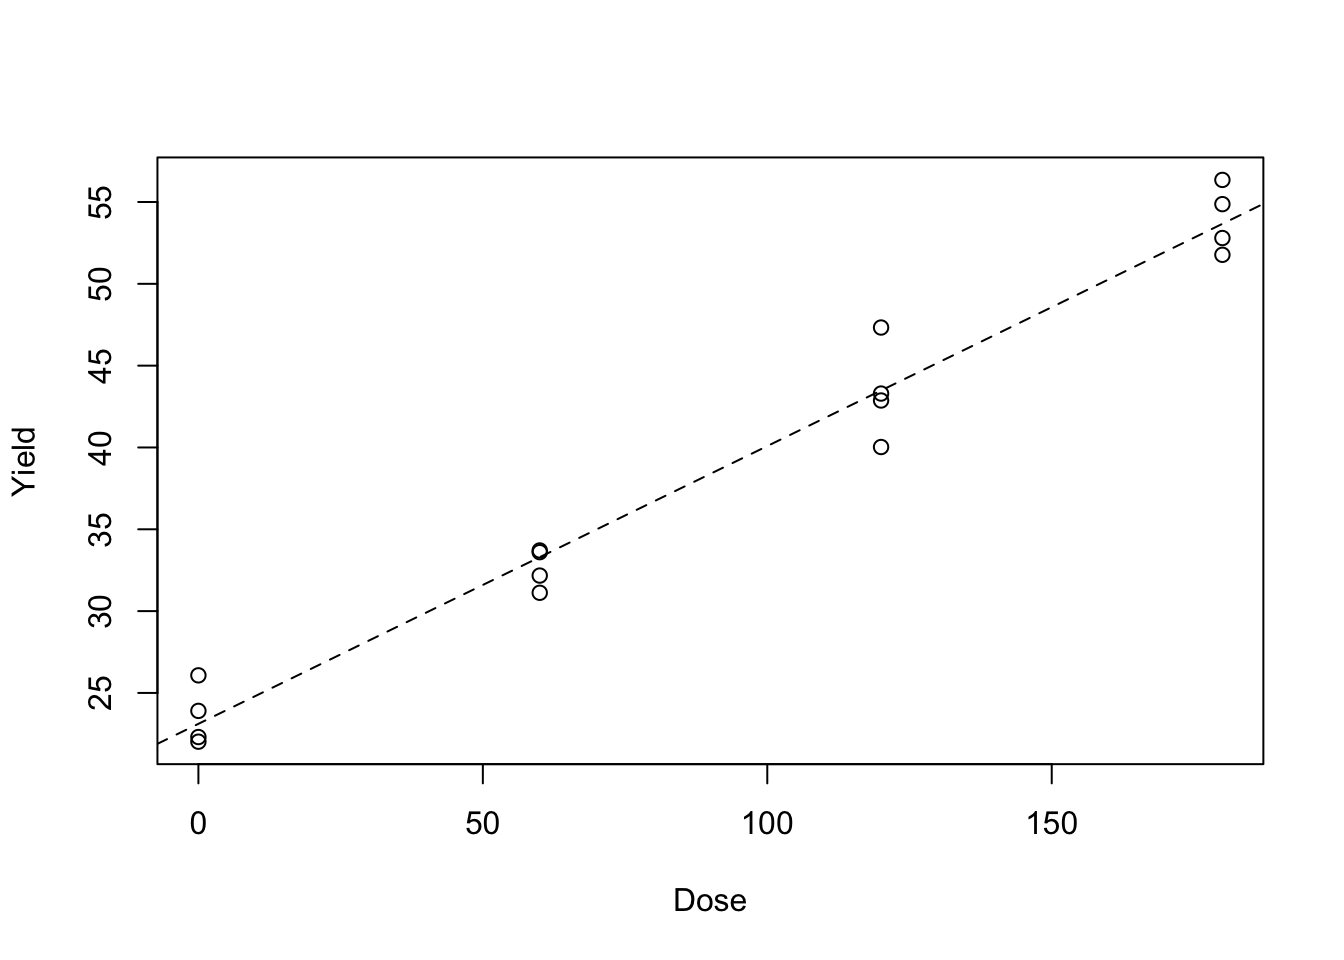
\includegraphics{_main_files/figure-latex/unnamed-chunk-139-1.pdf}

Il grafico suggerisce che la risposta della concentrazione nel tempo è
curvilinea, secondo la seguente equazione generale:

\[ Y = f(X, \theta) + \epsilon \]

dove \(X\) è il tempo, \(Y\) la concentrazione, \(\theta\) sono i
parametri del modello ed \(\epsilon\) sono i residui, che misurano lo
scostamento dei dati osservati dalla risposta attesa, secondo
l'equazione prescelta per \(f\). E' evidente che \(X\) ed \(Y\) sono
noti, ma resta da scegliere \(f\) e da stimare \(\theta\).

\subsection{Scelta della funzione}\label{scelta-della-funzione}

Uno dei criteri fondamentali, ancorché empirico, per la selezione di una
curva è quello di considerarne la forma, in relazione al fenomeno
biologico in studio. Secondo i testi più affidabili (Ratkowsky
\protect\hyperlink{ref-ratko1990Handbook}{1990}), le equazioni possono
essere classificate in:

\begin{itemize}
\tightlist
\item
  Curve Lineari

  \begin{enumerate}
  \def\labelenumi{\arabic{enumi}.}
  \tightlist
  \item
    Retta
  \item
    Parabola
  \end{enumerate}
\item
  Curve convesse/concave

  \begin{enumerate}
  \def\labelenumi{\arabic{enumi}.}
  \tightlist
  \item
    Funzione esponenziale
  \item
    Funzione di potenza
  \item
    Funzione logaritmica
  \item
    Iperbole rettangolare
  \item
    Funzione monomolecolare
  \item
    Funzione di Michaelis-Menten
  \end{enumerate}
\item
  Curve sigmoidali

  \begin{enumerate}
  \def\labelenumi{\arabic{enumi}.}
  \tightlist
  \item
    Funzione logistica
  \item
    Funzione di Gompertz
  \item
    Funzione 'valori estremi'
  \item
    Funzione Log-logistica (Equazione di Hill)
  \item
    Weibull-1 (log-Gompertz)
  \item
    Weibull-2 (log-Extreme)
  \end{enumerate}
\item
  Curve con massimi/minimi

  \begin{enumerate}
  \def\labelenumi{\arabic{enumi}.}
  \tightlist
  \item
    Equazione di Brain-Cousens
  \item
    Equazione di Braggs
  \end{enumerate}
\end{itemize}

La descrizione di queste curve verrà fatta in appendice. In questo caso
specifico abbiamo bisogno di una funzione concava verso l'alto e con un
asintoto orizzontale coincidente con l'asse delle X. Le conoscenze in
relazione alla cinetica di degradazione dei composti chimici ci
suggerisce una relazione esponenziale (cinetica del primo ordine), così
definita:

\[ Y = A e^{-k \,X} \]

dove A è la concentrazione iniziale e \(k\) e il tasso di degradazione
(costante nel tempo).

\subsection{Stima dei parametri}\label{stima-dei-parametri-3}

Dopo aver definito \(f\), dobbiamo stimare i parametri \(A\) e \(k\). In
generale esistono tre tecniche fondamentali (Draper and Smith
\protect\hyperlink{ref-draper1998_Appliedregressionanalysis}{1998}) :

\begin{enumerate}
\def\labelenumi{\arabic{enumi}.}
\tightlist
\item
  linearizzazione della funzione tramite trasformazione delle variabili;
\item
  approssimazione della vera funzione curvilinea con una polinomiale in
  X;
\item
  adattamento ai dati sperimentali di funzioni curvilinee, tramite
  metodiche di regressione non-lineare.
\end{enumerate}

\subsubsection{Linearizzazione della
funzione}\label{linearizzazione-della-funzione}

Nel caso specifico, prendendo il logaritmo di entrambe le parti
dell'equazione, otteniamo la seguente trasformazione:

\[ log(Y) = log(A) + X \]

Possiamo quindi trasformare la Y nel suo logaritmo ed utilizzare un
modello lineare per la stima dei parametri.

\begin{Shaded}
\begin{Highlighting}[]
\NormalTok{mod <-}\StringTok{ }\KeywordTok{lm}\NormalTok{(}\KeywordTok{log}\NormalTok{(Conc) }\OperatorTok{~}\StringTok{ }\NormalTok{Time, }\DataTypeTok{data=}\NormalTok{degradation)}
\KeywordTok{summary}\NormalTok{(mod)}
\NormalTok{## }
\NormalTok{## Call:}
\NormalTok{## lm(formula = log(Conc) ~ Time, data = degradation)}
\NormalTok{## }
\NormalTok{## Residuals:}
\NormalTok{##      Min       1Q   Median       3Q      Max }
\NormalTok{## -2.11738 -0.09583  0.05336  0.31166  1.01243 }
\NormalTok{## }
\NormalTok{## Coefficients:}
\NormalTok{##              Estimate Std. Error t value Pr(>|t|)    }
\NormalTok{## (Intercept)  4.662874   0.257325   18.12 1.04e-14 ***}
\NormalTok{## Time        -0.071906   0.006151  -11.69 6.56e-11 ***}
\NormalTok{## ---}
\NormalTok{## Signif. codes:  0 '***' 0.001 '**' 0.01 '*' 0.05 '.' 0.1 ' ' 1}
\NormalTok{## }
\NormalTok{## Residual standard error: 0.6905 on 22 degrees of freedom}
\NormalTok{## Multiple R-squared:  0.8613, Adjusted R-squared:  0.855 }
\NormalTok{## F-statistic: 136.6 on 1 and 22 DF,  p-value: 6.564e-11}
\end{Highlighting}
\end{Shaded}

Le funzioni linearizzabili per semplice trasformazione delle variabili
sono dette \emph{linearizzabili} e presentano il vantaggio di
semplificare molto i calcoli richiesti per la stima dei parametri. Un
grave svantaggio è dato dal fatto che trasformando la Y si trasforma
anche la distribuzione degli errori e quindi bisogna verificare che le
assunzioni di base dei modelli lineari (omogeneità delle varianze e
normalità dei residui) siano valide nella scala trasformata

\begin{Shaded}
\begin{Highlighting}[]
\KeywordTok{plot}\NormalTok{(}\KeywordTok{residuals}\NormalTok{(mod) }\OperatorTok{~}\StringTok{ }\KeywordTok{fitted}\NormalTok{(mod), }
     \DataTypeTok{xlab=}\StringTok{"Fitted data"}\NormalTok{, }\DataTypeTok{ylab=}\StringTok{"Residuals"}\NormalTok{)}
\KeywordTok{abline}\NormalTok{(}\DataTypeTok{h=}\DecValTok{0}\NormalTok{, }\DataTypeTok{lty=}\DecValTok{2}\NormalTok{)}
\end{Highlighting}
\end{Shaded}

\begin{figure}
\centering
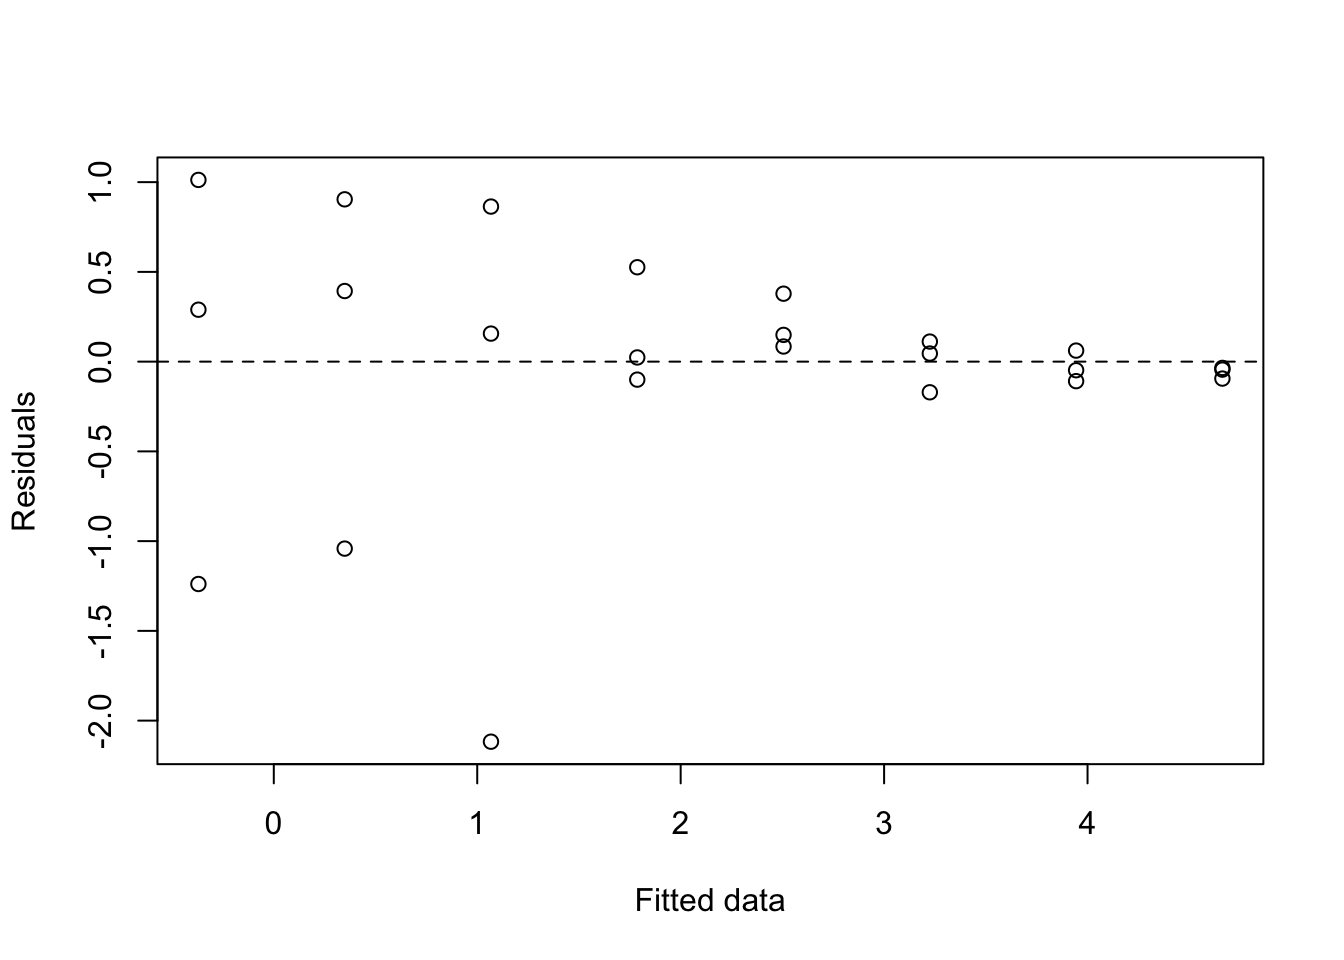
\includegraphics{_main_files/figure-latex/foo-1.pdf}
\caption{\label{fig:foo}Prova}
\end{figure}

In questo caso specifico, il grafico dei residui suggerisci deviazioni
consistenti rispetto alla omogeneità delle varianze, che risultano
inversamente proporzionali ai valori attesi (più alto il logaritmo della
concentrazione più bassi i residui). Questo fa sospettare che le
varianze potrebbero essere omogenee sulla scala originale, impedendoci
quindi di analizzare i dati nella scala trasformata.

\subsubsection{Approssimazione della vera funzione tramite una
polinomiale in
X}\label{approssimazione-della-vera-funzione-tramite-una-polinomiale-in-x}

In generale, relazioni matematiche curvilinee possono essere
approssimate tramite funzioni polinomiali di ordine \textit{n}. Le
funzioni polinomiali sono molto flessibili; contengono la funzione
lineare come caso particolare (n=1) e permette di descrivere curvature
anche molto complesse semplicemente aumentando l' ordine della funzione.
In questo modo è possibile ottenere un adattamento ai dati sperimentali
teoricamente anche perfetto.

Le funzioni polinomiali sono un tipico esempio di funzioni non-lineari
nelle variabili, ma lineari nei parametri; esse possono essere trattate
ricorrendo alle metodiche di calcolo normalmente utilizzate per la
regressione lineare.

Gli svantaggi delle funzioni polinomiali sono relativi al fatto che
queste presentano raramente giustificazione biologica. Per esempio, con
le funzioni polinomiali non è possibile descrivere relazioni
asintotiche, che sono invece molto comuni in biologia. Nel nostro
esempio si potrebbe utilizzare una funzione polinomiale di II grado.

\begin{Shaded}
\begin{Highlighting}[]
\NormalTok{mod2 <-}\StringTok{ }\KeywordTok{lm}\NormalTok{(Conc }\OperatorTok{~}\StringTok{ }\NormalTok{Time }\OperatorTok{+}\StringTok{ }\KeywordTok{I}\NormalTok{(Time}\OperatorTok{^}\DecValTok{2}\NormalTok{), }\DataTypeTok{data=}\NormalTok{degradation)}
\KeywordTok{plot}\NormalTok{(Conc }\OperatorTok{~}\StringTok{ }\NormalTok{Time, }\DataTypeTok{data=}\NormalTok{degradation)}
\NormalTok{coefs <-}\StringTok{ }\KeywordTok{coef}\NormalTok{(mod2)}
\KeywordTok{curve}\NormalTok{(coefs[}\DecValTok{1}\NormalTok{] }\OperatorTok{+}\StringTok{ }\NormalTok{coefs[}\DecValTok{2}\NormalTok{]}\OperatorTok{*}\NormalTok{x }\OperatorTok{+}\StringTok{ }\NormalTok{coefs[}\DecValTok{3}\NormalTok{]}\OperatorTok{*}\NormalTok{x}\OperatorTok{^}\DecValTok{2}\NormalTok{, }\DataTypeTok{add=}\NormalTok{T, }\DataTypeTok{col=}\StringTok{"red"}\NormalTok{)}
\end{Highlighting}
\end{Shaded}

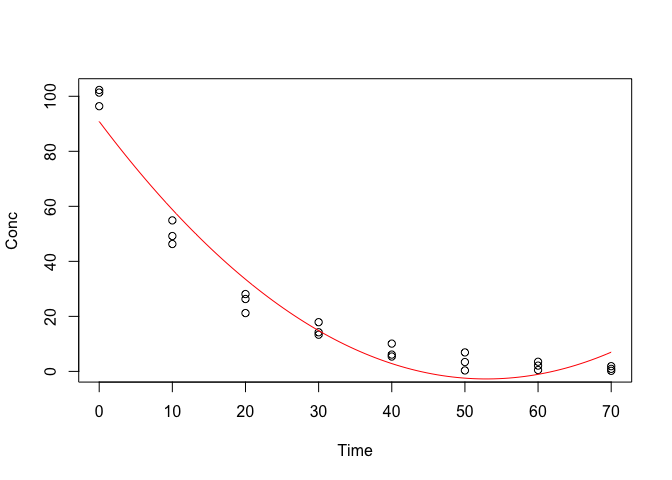
\includegraphics{_main_files/figure-latex/unnamed-chunk-141-1.pdf}

Vediamo come la funzione inserita, mentre approssima bene i dati
nell'intervallo da 0 a 40 giorni, successivamente mostra una ricrescita,
che non ha alcun senso biologico.

In generale, le polinomiali sono utilizzate quando sia necessario
approssimare una funzione curvilinea in un intervallo della X molto
ristretto e non consentono nessuna estrapolazione al di fuori di questo
intervallo, dato che possono portare a stime della risposta
completamente insensate biologicamente.

Per questi motivi l' uso delle funzioni polinomiali dovrebbe essere
limitato ai casi in cui non si abbia nessuna conoscenza \emph{a priori}
dell' andamento del fenomeno. Tra l' altro i moderni supporti
informatici consentono di risolvere il problema dell' adattamento
diretto di funzioni curvilinee qualunque senza i lunghi calcoli manuali
che venivano richiesti fino ad alcuni anni fa.

\subsubsection{Adattamento di funzioni curvilinee qualunque: regressione
non-lineare}\label{adattamento-di-funzioni-curvilinee-qualunque-regressione-non-lineare}

Per quanto sopra accennato, ogniqualvolta possibile, si preferisce
utilizzare metodologie di regressione non-lineare, che permettono di
adattare direttamente funzioni curvilinee di qualunque tipo ai dati
sperimentali. La stima dei parametri, tuttavia, non è immediata e
richiede l'impiego di metodi iterativi, come il metodo di Gauss-Newton
(Bates and Watts
\protect\hyperlink{ref-bates1988_Nonlinearregressionanalysis}{1988})
(Gauss-Newton, Steepest Descent, Marquardt, Simplex; alcune informazioni
sono riportate in appendice). In questo caso, è necessario fissare delle
stime iniziali dei parametri, che vengono corrette in ogni iterazione
successiva fino ad ottenere la convergenza sui valori che minimizzano lo
scostamento tra i dati osservati e la funzione non-lineare (metodo dei
minimi quadrati non-lineari). Ovviamente, trattandosi di metodi
iterativi, le stime ottenute sono solo un'approssimazione (accettabile!)
dei valori reali.

\subsection{La regressione non-lineare con
R}\label{la-regressione-non-lineare-con-r}

La funzione più comune in R per la parametrizzazione di funzioni
non-lineari è nls(), che è descritta in dettaglio da C. Ritz and
Streibig (\protect\hyperlink{ref-ritz2008_Nonlinearregression}{2008}).
Nella chiamata alla funzione dobbiamo anche fornire stime iniziali per i
valori dei parametri. Ottenere queste stime è facile pensando al
significato biologico dei parametri: \(A\) è la concentrazione iniziale
e quindi una stima ragionevole è data dal valor medio osservato al tempo
0 (100). Il parametro \(k\) è invece il tasso di degradazione relativo;
possiamo notare che nei primi 10 giorni la concentrazione si riduce
della metà circa, cioè si abbassa mediamente un po' più del 5\% al
giorno (considerando che inizialmente il calo è più rapido). Possiamo
quindi assegnare a \(k\) un valore iniziale pari a 0.06.

\begin{Shaded}
\begin{Highlighting}[]
\NormalTok{modNlin <-}\StringTok{ }\KeywordTok{nls}\NormalTok{(Conc }\OperatorTok{~}\StringTok{ }\NormalTok{A}\OperatorTok{*}\KeywordTok{exp}\NormalTok{(}\OperatorTok{-}\NormalTok{k}\OperatorTok{*}\NormalTok{Time), }
               \DataTypeTok{start=}\KeywordTok{list}\NormalTok{(}\DataTypeTok{A=}\DecValTok{100}\NormalTok{, }\DataTypeTok{k=}\FloatTok{0.06}\NormalTok{), }
               \DataTypeTok{data=}\NormalTok{degradation)}
\KeywordTok{summary}\NormalTok{(modNlin)}
\NormalTok{## }
\NormalTok{## Formula: Conc ~ A * exp(-k * Time)}
\NormalTok{## }
\NormalTok{## Parameters:}
\NormalTok{##    Estimate Std. Error t value Pr(>|t|)    }
\NormalTok{## A 99.634898   1.461047   68.19   <2e-16 ***}
\NormalTok{## k  0.067039   0.001887   35.53   <2e-16 ***}
\NormalTok{## ---}
\NormalTok{## Signif. codes:  0 '***' 0.001 '**' 0.01 '*' 0.05 '.' 0.1 ' ' 1}
\NormalTok{## }
\NormalTok{## Residual standard error: 2.621 on 22 degrees of freedom}
\NormalTok{## }
\NormalTok{## Number of iterations to convergence: 4 }
\NormalTok{## Achieved convergence tolerance: 1.549e-06}
\end{Highlighting}
\end{Shaded}

In alternativa, preferiamo utilizzare il package drc, con la funzione
drm(), che ha un'infrastruttura molto comoda per le regressioni
non-lineari in genere, compresa la definizione di funzioni di
self-starting, che ci liberano dal problema di dover reperire le stime
iniziali dei parametri (Christian Ritz et al.
\protect\hyperlink{ref-ritz2015_DoseResponseAnalysisUsing}{2015}). La
chiamata è simile a quella di nls(), anche se vengono indicate
separatamente le due variabili (Y \textasciitilde{} X) e la funzione (in
questo caso il nome è firstOrder()).

\begin{Shaded}
\begin{Highlighting}[]
\KeywordTok{library}\NormalTok{(drc)}
\NormalTok{modNlin2 <-}\StringTok{ }\KeywordTok{drm}\NormalTok{(Conc }\OperatorTok{~}\StringTok{ }\NormalTok{Time, }\DataTypeTok{fct=}\KeywordTok{DRC.expoDecay}\NormalTok{(),}
                \DataTypeTok{data=}\NormalTok{degradation)}
\KeywordTok{summary}\NormalTok{(modNlin2)}
\NormalTok{## }
\NormalTok{## Model fitted: Exponential Decay Model (2 parms)}
\NormalTok{## }
\NormalTok{## Parameter estimates:}
\NormalTok{## }
\NormalTok{##                    Estimate Std. Error t-value   p-value    }
\NormalTok{## init:(Intercept) 99.6349312  1.4646680  68.026 < 2.2e-16 ***}
\NormalTok{## k:(Intercept)     0.0670391  0.0019089  35.120 < 2.2e-16 ***}
\NormalTok{## ---}
\NormalTok{## Signif. codes:  0 '***' 0.001 '**' 0.01 '*' 0.05 '.' 0.1 ' ' 1}
\NormalTok{## }
\NormalTok{## Residual standard error:}
\NormalTok{## }
\NormalTok{##  2.621386 (22 degrees of freedom)}
\end{Highlighting}
\end{Shaded}

I risultati sono praticamente identici.

\section{Riparametrizzazione delle
funzioni}\label{riparametrizzazione-delle-funzioni}

In alcuni casi è conveniente riparametrizzare le funzioni, se è
necessario per le nostre esigenze di analisi. Anche questo aspetto sarà
illustrato con un esempio.

\subsection{Esempio 2}\label{esempio-2-2}

E'stata valutata la produzione del girasole a densità crescenti di
piante infestanti, da 0 a 100 piante per metro quadrato. I risultati
ottenuti sono riportati nel dataset sottostante.

\begin{Shaded}
\begin{Highlighting}[]
\KeywordTok{data}\NormalTok{(competition)}
\KeywordTok{head}\NormalTok{(competition)}
\NormalTok{##   Dens    Yield}
\NormalTok{## 1    0 29.58587}
\NormalTok{## 2   10 20.16776}
\NormalTok{## 3   20 17.82846}
\NormalTok{## 4   30  9.02289}
\NormalTok{## 5   40 13.41521}
\NormalTok{## 6   50 12.80159}
\end{Highlighting}
\end{Shaded}

Secondo la letteratura, la relazione tra perdite produttive e densità
delle piante infestanti può essere descritta con una funzione iperbolica
di questo tipo (Cousens, 1985):

\[YL = \frac{iD}{1 + \frac{iD}{a}}\]

Dove \(YL\) sta per perdite produttive (Yield Loss) percentuali, \(D\) è
la densità delle piante infestanti, \(a\) è la perdita produttiva
massima asintotica. Il grafico è mostrato qui sotto.

\begin{Shaded}
\begin{Highlighting}[]
\KeywordTok{curve}\NormalTok{(}\DecValTok{3}\OperatorTok{*}\NormalTok{x}\OperatorTok{/}\NormalTok{(}\DecValTok{1}\OperatorTok{+}\NormalTok{(}\DecValTok{3}\OperatorTok{*}\NormalTok{x)}\OperatorTok{/}\DecValTok{60}\NormalTok{), }\DataTypeTok{from=}\DecValTok{0}\NormalTok{, }\DataTypeTok{to=}\DecValTok{350}\NormalTok{, }\DataTypeTok{xlab=}\StringTok{"Weed density"}\NormalTok{,}
      \DataTypeTok{ylab=}\StringTok{"Yield loss (%)"}\NormalTok{, }\DataTypeTok{ylim=}\KeywordTok{c}\NormalTok{(}\DecValTok{0}\NormalTok{,}\DecValTok{80}\NormalTok{))}
\KeywordTok{abline}\NormalTok{(}\DataTypeTok{a=}\DecValTok{0}\NormalTok{, }\DataTypeTok{b=}\DecValTok{3}\NormalTok{, }\DataTypeTok{lty=}\DecValTok{2}\NormalTok{, }\DataTypeTok{ylim=}\KeywordTok{c}\NormalTok{(}\DecValTok{0}\NormalTok{,}\DecValTok{2}\NormalTok{))}
\KeywordTok{abline}\NormalTok{(}\DataTypeTok{h=}\DecValTok{60}\NormalTok{, }\DataTypeTok{lty=}\DecValTok{2}\NormalTok{, }\DataTypeTok{ylim=}\KeywordTok{c}\NormalTok{(}\DecValTok{0}\NormalTok{,}\DecValTok{2}\NormalTok{))}
\KeywordTok{text}\NormalTok{(}\DecValTok{20}\NormalTok{,}\DecValTok{50}\NormalTok{, }\DataTypeTok{label=}\StringTok{"i = 3"}\NormalTok{)}
\KeywordTok{text}\NormalTok{(}\DecValTok{300}\NormalTok{,}\DecValTok{65}\NormalTok{, }\DataTypeTok{label=}\StringTok{"A = 60"}\NormalTok{)}
\end{Highlighting}
\end{Shaded}

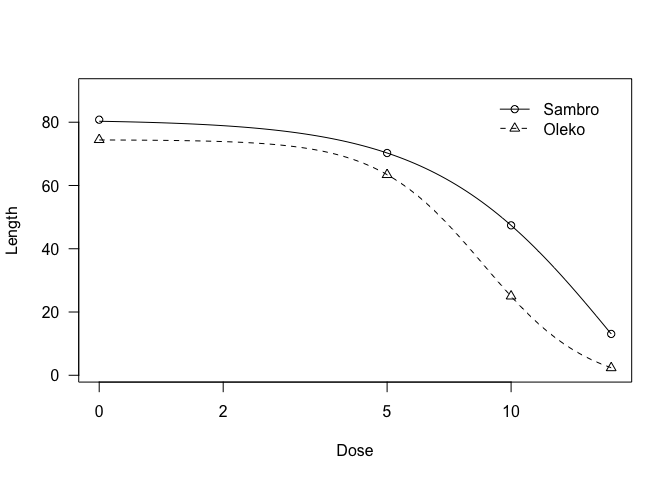
\includegraphics{_main_files/figure-latex/unnamed-chunk-145-1.pdf}

Normalmente, in campo non vengono determinate le perdite produttive,
bensì le produzioni, come nel caso del nostro dataset. Di conseguenza
abbiamo due possibilità:

\begin{enumerate}
\def\labelenumi{\arabic{enumi}.}
\tightlist
\item
  modificare il dataset, esprimendo i dati in termini di perdite
  produttive percentuali;
\item
  modificare il modello, per utilizzare la produzione come variabile
  dipendente, al posto della perdita produttiva.
\end{enumerate}

La prima strada è più agevole, ma ci porta a perdere parte
dell'informazione, cioè il livello produttivo nel testimone non
infestato. La seconda strada può essere perseguita considerando che le
perdite produttive percentuali sono pari a:

\[YL = \frac{{YWF - YW}}{{YWF}} \times 100\]

dove \(YWF\) è la produzione nel testimone non infestato e \(YW\) è la
produzione nella parcella in studio. Dalla precedente funzione si ricava
che:

\[YW = YWF - \frac{YL \times YWF}{100} = YWF\left( {1 - \frac{YL}{100}} \right)\]

che mostra come la produzione in una parcella infestata (\(YW\)) può
essere ottenuta in funzione della perdita produttiva. Considerando
l'equazione precedente e il modello delle perdite produttive, possiamo
scrivere:

\[YW = YWF\left( {1 - \frac{iD}{100\left( {1 + \frac{iD}{a}} \right)}} \right)\]

Questa equazione consente di utilizzare i dati produttivi osservati come
variabile dipendente e di stimare i parametri competitivi \(i\) ed
\(a\), insiema alla produzione stimata in asssenza di competizione. Il
fitting può essere eseguito utilizzando drm() e la funzione cousens85().

\begin{Shaded}
\begin{Highlighting}[]
\NormalTok{modComp <-}\StringTok{ }\KeywordTok{drm}\NormalTok{(Yield }\OperatorTok{~}\StringTok{ }\NormalTok{Dens, }\DataTypeTok{fct=}\KeywordTok{DRC.cousens85}\NormalTok{() ,}
               \DataTypeTok{data=}\NormalTok{competition)}
\KeywordTok{summary}\NormalTok{(modComp)}
\NormalTok{## }
\NormalTok{## Model fitted: Yield-Weed Density function (Cousens, 1985) (3 parms)}
\NormalTok{## }
\NormalTok{## Parameter estimates:}
\NormalTok{## }
\NormalTok{##                 Estimate Std. Error t-value   p-value    }
\NormalTok{## YWF:(Intercept) 30.47211    0.92763 32.8493 < 2.2e-16 ***}
\NormalTok{## i:(Intercept)    8.24038    1.36541  6.0351 3.857e-07 ***}
\NormalTok{## a:(Intercept)   75.07312    2.40366 31.2328 < 2.2e-16 ***}
\NormalTok{## ---}
\NormalTok{## Signif. codes:  0 '***' 0.001 '**' 0.01 '*' 0.05 '.' 0.1 ' ' 1}
\NormalTok{## }
\NormalTok{## Residual standard error:}
\NormalTok{## }
\NormalTok{##  1.866311 (41 degrees of freedom)}
\end{Highlighting}
\end{Shaded}

\section{Inferenze statistiche e verifiche delle assunzioni di
base}\label{inferenze-statistiche-e-verifiche-delle-assunzioni-di-base}

Le assunzioni parametriche di base relative ai modelli non-lineari sono
le stesse dei modelli lineari e, di conseguenza, gli strumenti
diagnostici sono analoghi. Bisogna tuttavia menzionare il fatto che,
dato l'impiego di metodi iterativi per la ricerca dei valori dei
parametri, tutti i risultati a cui si perviene (stima dei parametri,
della varianza residua e numero dei gradi di libertà relativi) sono solo
una approssimazione di quelli reali. Per questo motivo, nel caso
non-lineare i metodi grafici (analisi dei residui) sono largamente
preferiti.

\subsection{Analisi grafica dei
residui}\label{analisi-grafica-dei-residui-1}

I due strumenti grafici preferiti sono la visualizzazione della funzione
insieme ai dati osservati e la visualizzazione dei residui, plottati
verso i valori attesi. Avendo utilizzato la funzione drm(), possiamo
approfittare dell'oggetto risultante per disegnare i grafici.
Considerate che la funzione plot() applicata all'oggetto drm restituisce
di default un grafico sul logaritmo della variabile indipendente. In
questo caso abbiamo ovviato a questo comportamento utilizzando la
funzione log=``''.

Consideriamo i due esempi precedenti.

\begin{Shaded}
\begin{Highlighting}[]
\KeywordTok{par}\NormalTok{(}\DataTypeTok{mfrow=}\KeywordTok{c}\NormalTok{(}\DecValTok{1}\NormalTok{,}\DecValTok{2}\NormalTok{))}
\KeywordTok{plot}\NormalTok{(modNlin2, }\DataTypeTok{log=}\StringTok{""}\NormalTok{)}
\KeywordTok{plot}\NormalTok{(}\KeywordTok{residuals}\NormalTok{(modNlin2) }\OperatorTok{~}\StringTok{ }\KeywordTok{fitted}\NormalTok{(modNlin2))}
\KeywordTok{abline}\NormalTok{(}\DataTypeTok{h=}\DecValTok{0}\NormalTok{, }\DataTypeTok{lty=}\DecValTok{2}\NormalTok{)}
\end{Highlighting}
\end{Shaded}

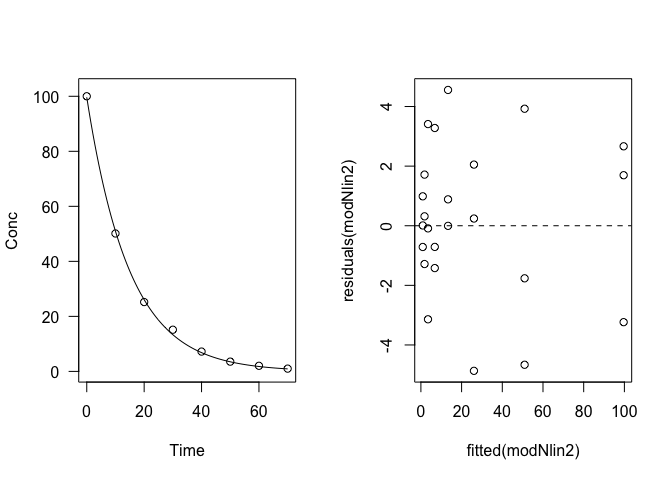
\includegraphics{_main_files/figure-latex/unnamed-chunk-147-1.pdf}

Nel caso dell'esempio relativo alla cinetica di degradazione, non si
vedono importanti deviazioni rispetto agli assunti di base.

\begin{Shaded}
\begin{Highlighting}[]
\KeywordTok{par}\NormalTok{(}\DataTypeTok{mfrow=}\KeywordTok{c}\NormalTok{(}\DecValTok{1}\NormalTok{,}\DecValTok{2}\NormalTok{))}
\KeywordTok{plot}\NormalTok{(modComp, }\DataTypeTok{log=}\StringTok{""}\NormalTok{)}
\KeywordTok{plot}\NormalTok{(}\KeywordTok{residuals}\NormalTok{(modComp) }\OperatorTok{~}\StringTok{ }\KeywordTok{fitted}\NormalTok{(modComp))}
\KeywordTok{abline}\NormalTok{(}\DataTypeTok{h=}\DecValTok{0}\NormalTok{, }\DataTypeTok{lty=}\DecValTok{2}\NormalTok{)}
\end{Highlighting}
\end{Shaded}

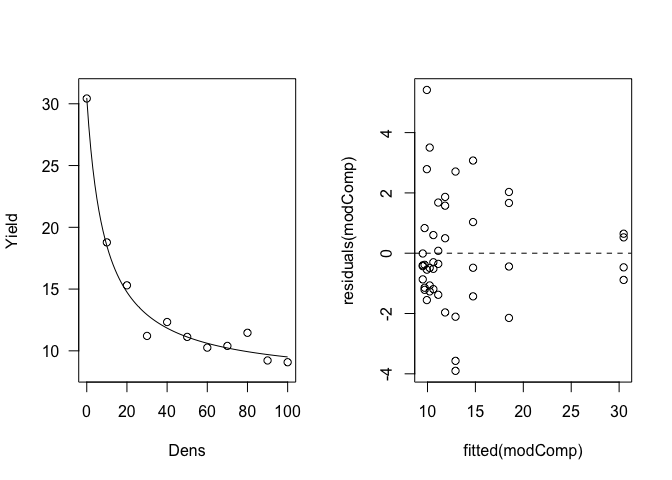
\includegraphics{_main_files/figure-latex/unnamed-chunk-148-1.pdf}

Per quello che riguarda il modello di competizione, osserviamo invece
una proporzionalità inversa tra residui e medie, che attesta qualche
problema con l'omogeneità delle varianze.

\subsection{Test F per la mancanza di adattamento
(approssimato)}\label{test-f-per-la-mancanza-di-adattamento-approssimato}

Se abbiamo le repliche (come nei due esempi fin qui trattati) possiamo
effettuare l'analisi della varianza. In questo modello, i valori attesi
sono costituiti dalle medie dei trattamenti (tempi e livelli di densità,
rispettivamente per i due esempi) e lo scostamento di ogni dato rispetto
alla `sua' media è evidentemente dovuto solo all'errore sperimentale
`puro'. Nel modello di regressione, invece, esiste una componente
aggiuntiva di errore, cioè lo scostamento di ogni media dalla curva di
regressione. Questa componente si chiama mancanza d'adattamento e può
essere stimata per differenza. Effettuiamo il calcolo per il primo
esempio.

La tabella ANOVA è la seguente:

\begin{Shaded}
\begin{Highlighting}[]
\NormalTok{modAov <-}\StringTok{ }\KeywordTok{lm}\NormalTok{(Conc }\OperatorTok{~}\StringTok{ }\KeywordTok{factor}\NormalTok{(Time), }\DataTypeTok{data=}\NormalTok{degradation)}
\KeywordTok{anova}\NormalTok{(modAov)}
\NormalTok{## Analysis of Variance Table}
\NormalTok{## }
\NormalTok{## Response: Conc}
\NormalTok{##              Df  Sum Sq Mean Sq F value    Pr(>F)    }
\NormalTok{## factor(Time)  7 24698.4  3528.3  415.29 < 2.2e-16 ***}
\NormalTok{## Residuals    16   135.9     8.5                      }
\NormalTok{## ---}
\NormalTok{## Signif. codes:  0 '***' 0.001 '**' 0.01 '*' 0.05 '.' 0.1 ' ' 1}
\NormalTok{SSa <-}\StringTok{ }\KeywordTok{anova}\NormalTok{(modAov)[}\DecValTok{2}\NormalTok{,}\DecValTok{2}\NormalTok{]}
\end{Highlighting}
\end{Shaded}

Inseriamo il tempo come fattore (quindi variabile qualitativa, non
quantitativa) e notiamo che la devianza del residuo è pari a 135.9.
Salviamo questa quantità nella variabile SSa. La varianza del residuo
del modello di regressione si ottiene facendo la somma dei quadrati
degli scarti dei dati rispetto ai valori attesi. La salviamo nella
variabile SSr.

\begin{Shaded}
\begin{Highlighting}[]
\NormalTok{SSr <-}\StringTok{ }\KeywordTok{sum}\NormalTok{(}\KeywordTok{residuals}\NormalTok{(modNlin2)}\OperatorTok{^}\DecValTok{2}\NormalTok{)}
\NormalTok{SSr}
\NormalTok{## [1] 151.1766}
\end{Highlighting}
\end{Shaded}

Come ci aspettavamo, il modello di regressione ha una devianza più alta,
in quanto questa contiene la componente di mancanza d'adattamento, pari
alla differenza tra SSa e SSr, cioè:

\begin{Shaded}
\begin{Highlighting}[]
\NormalTok{SSl <-}\StringTok{ }\NormalTok{SSr }\OperatorTok{-}\StringTok{ }\NormalTok{SSa}
\NormalTok{SSl}
\NormalTok{## [1] 15.23792}
\end{Highlighting}
\end{Shaded}

Mentre la devianza del residuo dell'ANOVA ha 16 gradi di libertà, quella
del residuo della regression ha N - P = 22, gradi di libertà, dove N è
il numero dei dati (24) e P è il numero dei parametri stimati (2). La
devianza del `lack of fit' ha quindi 22 - 16 = 6 gradi di libertà. La
varianza del lack of fit è quindi pari a:

\begin{Shaded}
\begin{Highlighting}[]
\NormalTok{SSl}\OperatorTok{/}\DecValTok{6}
\NormalTok{## [1] 2.539654}
\end{Highlighting}
\end{Shaded}

Possiamo quindi confrontare formalmente, con un test di F, le due
varianze dell'errore puro (dall'ANOVA: 8.5) e quella della mancanza di
adattamento, per vedere se quest'ultima è significativamente più
`grande' di quella dell'errore puro. L'ipotesi nulla è che la mancanza
d'adattamento non è rilevante ed il test di F è:

\begin{Shaded}
\begin{Highlighting}[]
\NormalTok{(Fvalue <-}\StringTok{ }\NormalTok{(SSl}\OperatorTok{/}\DecValTok{6}\NormalTok{) }\OperatorTok{/}\StringTok{ }\KeywordTok{anova}\NormalTok{(modAov)[}\DecValTok{2}\NormalTok{,}\DecValTok{3}\NormalTok{]) }\CommentTok{#F value}
\NormalTok{## [1] 0.2989175}
\KeywordTok{pf}\NormalTok{(}\FloatTok{0.2989}\NormalTok{, }\DecValTok{6}\NormalTok{, }\DecValTok{16}\NormalTok{, }\DataTypeTok{lower.tail=}\NormalTok{F)}
\NormalTok{## [1] 0.07155798}
\end{Highlighting}
\end{Shaded}

Chiaramente il test è non significativo.

A questo risultato si arriva facilmente utilizzando la funzione
modelFit(), applicata all'oggetto drm.

\begin{Shaded}
\begin{Highlighting}[]
\KeywordTok{modelFit}\NormalTok{(modNlin2)}
\NormalTok{## Lack-of-fit test}
\NormalTok{## }
\NormalTok{##           ModelDf    RSS Df F value p value}
\NormalTok{## ANOVA          16 135.94                   }
\NormalTok{## DRC model      22 151.18  6  0.2989  0.9284}
\end{Highlighting}
\end{Shaded}

Per il secondo esempio abbiamo

\begin{Shaded}
\begin{Highlighting}[]
\KeywordTok{modelFit}\NormalTok{(modComp)}
\NormalTok{## Lack-of-fit test}
\NormalTok{## }
\NormalTok{##           ModelDf    RSS Df F value p value}
\NormalTok{## ANOVA          33 116.95                   }
\NormalTok{## DRC model      41 142.81  8  0.9119  0.5188}
\end{Highlighting}
\end{Shaded}

\subsection{Errori standard dei
parametri}\label{errori-standard-dei-parametri-1}

Un'altra valutazione importante da fare è quella relativa agli errori
standard delle stime dei parametri, che non debbono mai essere superiori
alla metà del valore del parametro stimato, cosa che in questo caso è
pienamente verificata. Se così non fosse, l'intervallo di confidenza del
parametro conterrebbe lo zero, il che equivale a dire che il valore
stimato non sarebbe significativamente diverso da zero. Di conseguenza,
avere, per esempio, un `rate' non diverso da zero significherebbe che di
fatto la degradazione non avviene o comunque non è descrivibile con il
modello proposto.

\subsection{Coefficiente di
determinazione}\label{coefficiente-di-determinazione}

Abbiamo visto che il residuo della regressione è pari a 151.2 con 16
gradi di libertà. La devianza totale dei dati (somma dei quadrati degli
scarti rispetto alla media generale) è invece:

\begin{Shaded}
\begin{Highlighting}[]
\NormalTok{SSt <-}\StringTok{ }\KeywordTok{deviance}\NormalTok{(}\KeywordTok{lm}\NormalTok{(Conc }\OperatorTok{~}\StringTok{ }\DecValTok{1}\NormalTok{, }\DataTypeTok{data=}\NormalTok{degradation))}
\end{Highlighting}
\end{Shaded}

ed ha 23 gradi di libertà. La differenza:

\begin{Shaded}
\begin{Highlighting}[]
\NormalTok{SSt }\OperatorTok{-}\StringTok{ }\NormalTok{SSr}
\NormalTok{## [1] 24683.13}
\end{Highlighting}
\end{Shaded}

costituisce la devianza spiegata dalla regressione. Il coefficente di
determinazione \(R^2\) è quindi:

\[R^2 = \frac{SSt - SSr}{SSt} = \frac{24683.13}{24834.3} = 0.994\]

Che attesta un ottimo adattamento, in quanto è vicino ad 1. Bisogna
ricordare che, pur essendo utilizzato in modo pressoché ubiquitario, il
coefficiente di determinazione per i modelli nonlineari fornisce solo
un'indicazione abbastanza grezza sulla bontà del modello. Infatti:

\begin{enumerate}
\def\labelenumi{\arabic{enumi}.}
\tightlist
\item
  valori bassi possono essere ottenuti non solo perché la devianza della
  regressione è bassa, ma anche perché la devianza totale delle
  osservazioni è alta (molti dati e molto variabili).
\item
  L' \(R^2\) dipende dall'intervallo di variazione della variabile
  indipendente; di conseguenza, se nella regressione aggiungiamo uno o
  più livelli della X, otteniamo un innalzamento del valore di \(R^2\),
  che tuttavia non necessariamente produce un miglior modello. In questo
  caso, ad esempio, se la semivita è pari a 10 giorni, un esperimento
  con 0, 20, 40 e 80 giorni darà sicuramente valori di \(R^2\) più alti
  che non un esperimento con 5, 10, 20 e 40 giorni, anche se non
  necessariamente la bontà di adattamento è migliore.
\item
  Il coefficiente di determinazione è sensibile al numero di variabili
  esplicative presenti nel modello, e quindi non premia i modelli più
  semplici (viola quindi il principio del `rasoio di Occam').
\item
  Il coefficiente di determinazione è sensibile al numero di parametri
  presenti nel modello. Modelli con molti parametri danno sempre valori
  di \(R^2\) alti, ma non rispettano spesso le caratteristiche di
  semplicità e senso biologico che sono invece richieste ad un buon
  modello (anche qui una netta violazione del rasoio di Occam.
\end{enumerate}

\subsection{Coefficiente di determinazione
aggiustato}\label{coefficiente-di-determinazione-aggiustato}

Per evitare almeno gli ultimi due problemi, viene proposto il
coefficiente di determinazione corretto, dato dalla proporzione di
varianza (MS) spiegata dalla regressione:

\[R_a^2  = 1 - \frac{MS_{residuo} }{MS_{tot} }\]

Dato che dalle devianze si passa alle varianze, il valore di R\(^2\)
corretto è detto anche `R\(^2\) corretto per i gradi di libertà'. Il suo
rapporto con il coefficiente di determinazione tradizionale è:

\[ R_a^2  = 1 - \frac{\left( {1 - R^2 } \right)\left( {n - 1} \right)}{\left( {n - k - 1} \right)} \]

dove \(n\) è il numero di osservazioni e \(k\) il numero dei regressori.
L'\(R^2\) corretto è sempre più basso dell \(R^2\) e diminuisce con
l'aggiunta al modello di un nuovo regressore se l'incremento di devianza
totale è meno che quello della devianza residua. Può assumere valori
negativi se la varianza del residuo è maggiore della varianza della
variabile dipendente.

\subsection{Altre statistiche}\label{altre-statistiche}

Altri indicatori di bontà di adattamento molto usati in letteratura per
finalità puramente descrittive sono il Mean Square Error:

\[MSE = \frac{1}{N}\sum\limits_{i = 1}^N {(Y_i  - } \widehat{Y_i })^2\]

che, nel caso in esempio, è pari a 6.299.

Come vediamo si tratta della varianza del residuo, ma ottenuta divedendo
per il numero dei dati e non per il numero dei gradi di libertà
(varianza della popolazione e non varianza del campione). E'quindi un
indicatore inferenziale distorto, ma è importante consocerlo perché
viene spesso utilizzato per stabilire la bontà d'adattamento e il valore
predittivo di modelli deterministici.

Il MSE è spesso difficile da valutare perché, essendo una somma di
quadrati, la sua unità di misura non è quella dei dati. Per questo
motivo, spesso si utilizza la sua radice quadrata:

\[RMSE = \sqrt{MSE}\]

che ha la stessa unità di misura delle osservazioni. In questo caso, il
RRMSE (Root Mean Square Error) è uguale a 2.510, che, considerando i
dati ,rappresenta un valore decisamente basso.

Una variante molto utilizzata è il Relative Root Mean Square Error
(RRMSE):

\[RRMSE = \frac{\sqrt{MSE}} {\overline{Y}} \times 100\]

dove \(\overline{Y}\) è la media dei dati. Si tratta di un indicatore
analogo al coefficiente di variabilità, nel quale la bontà del modello
viene espressa relativamente alla media delle previsioni. Nel nostro
caso è pari al 9.8\%.

\section{\texorpdfstring{Gestione delle situazioni
`patologiche'}{Gestione delle situazioni patologiche}}\label{gestione-delle-situazioni-patologiche}

In alcuni casi la verifica della bontà del modello mette in luce
situazioni patologiche. In particolare potrebbe capitare che il modello
non sia adatto ai dati, o, al contrario, che i dati non siano adatti al
modello. Nel primo caso è necessario trasformare il modello, mentre nel
secondo caso l'azione più comune è quella di trasformare i dati.

\subsection{Trasformazione del
modello}\label{trasformazione-del-modello}

La trasformazione del modello dalla sua forma originaria in una forma
alternativa può rendersi necessaria per diversi motivi:

\begin{enumerate}
\def\labelenumi{\arabic{enumi}.}
\tightlist
\item
  il modello non presenta un buon adattamento ai dati sperimentali e
  l'analisi dei residui suggerisce deviazioni sistematiche. Per esempio,
  in una curva dose risposta può capitare che i residui siano
  prevalentemente positivi nella parte iniziale, facendo sospettare un
  effetto stimolante a basse dosi. Questo effetto non può essere
  descritto con una funzione sigmoidale, ma richiede un modello divsero,
  caratterizzato da un picco iniziale.
\item
  Alcuni parametri non sono significativamente diversi da zero, o non
  sono ben stimati, o assumono valori biologicamente irrealistici. In
  questo caso si può considerare la loro eliminazione dal modello, se è
  possibile. In alternativa, si può considerare la possibilità di
  imporre un vincolo, cioè sostituire il parametro con un valore
  arbitrario biologicamente ragionevole. Quest' ultima soluzione è
  tuttavia da considerare con attenzione e buon senso, proprio per la
  sua arbitrarietà.
\item
  Alta correlazione tra i parametri. Questa situazione fa sospettare che
  il modello sia troppo complesso (troppi parametri) e quindi non
  supportato dai dati. In questo caso bisognerebbe verificare se e come
  sia possibile utilizzare un modello più semplice.
\end{enumerate}

\subsection{Trasformazione dei dati}\label{trasformazione-dei-dati}

Se non è il modello ad essere mal definito, ma sono invece i dati a non
conformarsi alle assunzioni di base della regressione, è necessarip
valutare l'esigenza di una trasformazione stabilizzante. Nel caso
dell'Esempio 2 la possibile eterogeneità delle varianze può spingerci a
valutare l'impiego della famiglia di trasformazioni descritta da Box e
Cox (Box and Cox
\protect\hyperlink{ref-box1964_analysistransformations}{1964}). L'unica
differenza rispetto alle regressioni lineari è nel fatto che operare la
trasformazione della sola variabile dipendente comporta anche la
modifica della scala sulla quale vengono stimati i parametri, che quindi
non conservano il loro valore biologico. Ad esempio, nel modello di
competizione, il parametro \(a\) è la perdita produttiva massima
percentuale. Tuttavia, se dovessimo trasformare i dati nel logaritmo
prima dell'analisi il parametro \(a\) non conserverebbe il suo
significato biologico.

Per questo motivo, dato che spesso le regressioni non-lineari vengono
eseguite proprio perchè si è interessati all'informazione contenuta nei
parametri di un modello, si preferisce adottare la cosiddetta tecnica
della ``trasformazione di entrambe le parti'', o metodo TBS (``Transform
Both Sides'') e trasformare quindi sia i dati osservati per la variabile
dipendente, sia il modello (Carroll and Ruppert
\protect\hyperlink{ref-carroll1988_Transformationweightingregression}{1988}):

\[Y^\lambda  = f(X)^\lambda\]

In questo modo si ottengono i parametri della funzione sulla scala
originale come se la trasformazione non fosse stata eseguita per niente.

Se abbiamo utilizzato la funzione drm() per il fitting, possiamo
utilizzare la funzione boxcox(), che confronta la verosimiglianza dei
modelli ottenuti variando il valore di \(\lambda\) da -2 a 2. Questa
funzione applicata al modello di competizione mostra che il massimo di
verosimiglianza si ottiene proprio con \(\lambda\) = 1, cioè a dire che
la trasformazione non è affatto necessaria.

\begin{Shaded}
\begin{Highlighting}[]
\KeywordTok{boxcox}\NormalTok{(modComp)}
\end{Highlighting}
\end{Shaded}

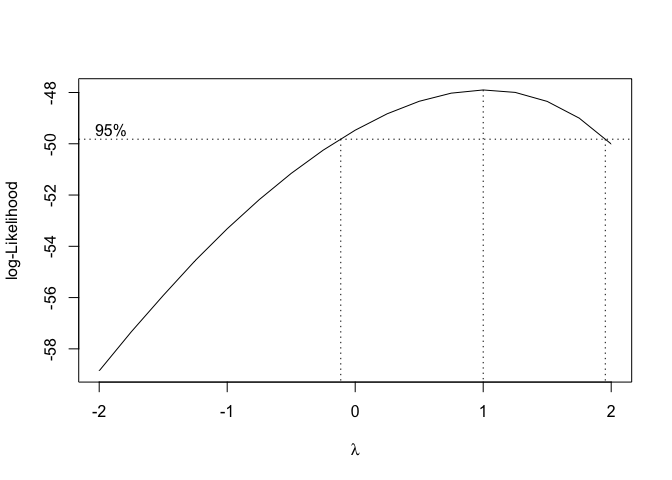
\includegraphics{_main_files/figure-latex/unnamed-chunk-158-1.pdf}

Se lo fosse, applicarla sarebbe banale: basterebbe aggiungere alla
funzione di fitting l'argomento bcVal, a cui si dovrebbe assegnare il
valore da utilizzare per la trasformazione.

\begin{Shaded}
\begin{Highlighting}[]
\NormalTok{modComp2 <-}\StringTok{ }\KeywordTok{drm}\NormalTok{(Yield }\OperatorTok{~}\StringTok{ }\NormalTok{Dens, }\DataTypeTok{fct=}\KeywordTok{DRC.cousens85}\NormalTok{(), }\DataTypeTok{data=}\NormalTok{competition,}
               \DataTypeTok{bcVal=}\FloatTok{0.5}\NormalTok{)}
\KeywordTok{summary}\NormalTok{(modComp2)}
\NormalTok{## }
\NormalTok{## Model fitted: Yield-Weed Density function (Cousens, 1985) (3 parms)}
\NormalTok{## }
\NormalTok{## Parameter estimates:}
\NormalTok{## }
\NormalTok{##                 Estimate Std. Error t-value   p-value    }
\NormalTok{## YWF:(Intercept)  30.5155     1.4523 21.0114 < 2.2e-16 ***}
\NormalTok{## i:(Intercept)     8.4999     1.7141  4.9589  1.28e-05 ***}
\NormalTok{## a:(Intercept)    75.0527     2.4308 30.8762 < 2.2e-16 ***}
\NormalTok{## ---}
\NormalTok{## Signif. codes:  0 '***' 0.001 '**' 0.01 '*' 0.05 '.' 0.1 ' ' 1}
\NormalTok{## }
\NormalTok{## Residual standard error:}
\NormalTok{## }
\NormalTok{##  0.5315512 (41 degrees of freedom)}
\NormalTok{## }
\NormalTok{## Non-normality/heterogeneity adjustment through Box-Cox transformation}
\NormalTok{## }
\NormalTok{## Specified lambda: 0.5}
\end{Highlighting}
\end{Shaded}

Vediamo che, nonostante la trasformazione, i parametri conservano il
loro significato biologico.

\section{Funzioni lineari e nonlineari dei
parametri}\label{funzioni-lineari-e-nonlineari-dei-parametri}

Gli studi di degradazione, in genere, richiedono la determinazione della
semivita. E'facile vedere che questa può essere ricavata dalla funzione
di degradazione in questo modo:

\[ \frac{A}{2} = A \exp ( - k \,\, t_{1/2}) \]

da cui:

\[ t_{1/2} = - \frac{ \log \left( {\frac{1}{2}} \right) }{k}\]

Vediamo insomma che la semivita \(t_{1/2}\) è una funzione non-lineare
di k e può essere ricavata facilmente come:

\begin{Shaded}
\begin{Highlighting}[]
\OperatorTok{-}\KeywordTok{log}\NormalTok{(}\DecValTok{1}\OperatorTok{/}\DecValTok{2}\NormalTok{) }\OperatorTok{/}\StringTok{ }\KeywordTok{coef}\NormalTok{(modNlin2)[}\DecValTok{2}\NormalTok{]}
\NormalTok{## k:(Intercept) }
\NormalTok{##      10.33945}
\end{Highlighting}
\end{Shaded}

Si pone ora il problema di ricavare l'errore standard della semivita e/o
i suoi intervalli di confidenza. La legge di propagazione degli errori
ci insegna che se abbiamo una quantità \(Z\) con varianza \(\sigma^2_Z\)
e facciamo una trasformazione lineare:

\[W = b_0 + b_1 \,\, Z\]

con \(b_0\) e \(b_1\) numeri reali qualunque, la varianza di W è data
da:

\[\sigma^2_W = b_1^2 \,\, \sigma^2_Z\]

In questo caso, purtroppo, la funzione di trasformazione è non lineare.
Tuttavia, una funzione non-lineare (ma vicina alla linearità) può essere
approssimata utilizzando la sua tangente in un punto dato (sviluppo in
serie di Taylor; Fig 1).

\begin{Shaded}
\begin{Highlighting}[]
\KeywordTok{curve}\NormalTok{(}\OperatorTok{-}\KeywordTok{log}\NormalTok{(}\DecValTok{1}\OperatorTok{/}\DecValTok{2}\NormalTok{)}\OperatorTok{/}\NormalTok{x, }\DataTypeTok{from=}\FloatTok{0.05}\NormalTok{, }\DataTypeTok{to=}\FloatTok{0.1}\NormalTok{)}
\KeywordTok{curve}\NormalTok{(}\KeywordTok{log}\NormalTok{(}\DecValTok{1}\OperatorTok{/}\DecValTok{2}\NormalTok{)}\OperatorTok{/}\NormalTok{(}\FloatTok{0.067}\OperatorTok{^}\DecValTok{2}\NormalTok{)}\OperatorTok{*}\NormalTok{(x }\OperatorTok{-}\StringTok{ }\FloatTok{0.067}\NormalTok{) }\OperatorTok{+}\StringTok{ }
\StringTok{        }\FloatTok{10.35}\NormalTok{, }\DataTypeTok{from=}\FloatTok{0.067}\NormalTok{, }\DataTypeTok{to=}\FloatTok{0.1}\NormalTok{, }\DataTypeTok{add=}\NormalTok{T, }\DataTypeTok{lty=}\DecValTok{1}\NormalTok{)}
\end{Highlighting}
\end{Shaded}

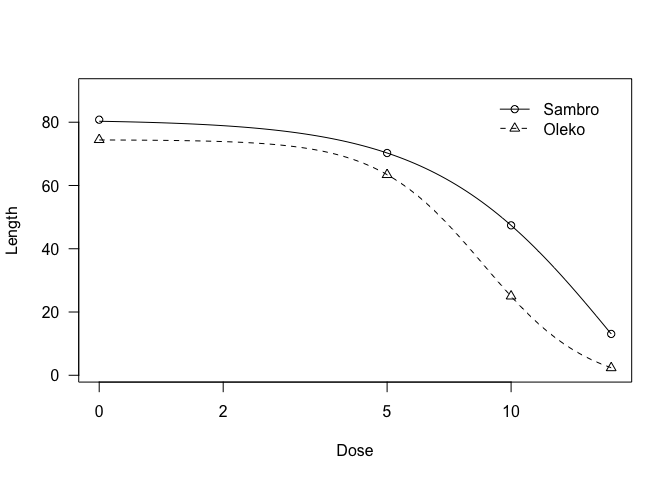
\includegraphics{_main_files/figure-latex/unnamed-chunk-161-1.pdf}

Consideriamo il punto \(k = 0.067\), dove la funzione vale
\(t_{1/2} = 10.35\). Immaginiamo di prendere la retta tangente nel punto
P(0.067, 10.35), questa retta ha equazione:

\[ y = m (x - x_0) + y_0 \]

dove m è la derivata prima della funzione nel punto \(k=0.067\):

\[ m = f'(k) = \frac{log(1/2)}{k^2}\]

Nei dintorni di 0.067 le due funzioni (quella nonlineare e la sua
tangente) sono molto vicine, quasi equivalenti. Allora posso pensare di
utilizzare la tangente per applicare la legge di propagazione degli
errori. Di conseguenza, la varianza della semivita è data da:

\[\sigma^2_{t_{1/2}} = m^2 \,\, \sigma^2_k\]

e l'errore standard è:

\[\frac{|log(1/2)|}{0.067^2} \,\, 0.0019 = 0.2944\]

Ovviamente, in R, possiamo utilizzare la funzione deltaMethod() del
package car, per arrivare agli stessi risultati.

\begin{Shaded}
\begin{Highlighting}[]
\KeywordTok{library}\NormalTok{(car)}
\NormalTok{coefs <-}\StringTok{ }\KeywordTok{coef}\NormalTok{(modNlin2) }
\KeywordTok{names}\NormalTok{(coefs) <-}\StringTok{ }\KeywordTok{c}\NormalTok{(}\StringTok{"A"}\NormalTok{, }\StringTok{"k"}\NormalTok{)}
\KeywordTok{deltaMethod}\NormalTok{(}\DataTypeTok{object=}\NormalTok{coefs, }\DataTypeTok{g=}\StringTok{"-log(0.5)/k"}\NormalTok{, }\DataTypeTok{vcov.=}\KeywordTok{vcov}\NormalTok{(modNlin2))}
\NormalTok{##             Estimate        SE    2.5 %   97.5 %}
\NormalTok{## -log(0.5)/k 10.33945 0.2944068 9.762424 10.91648}
\end{Highlighting}
\end{Shaded}

\section{Modelli ANCOVA}\label{modelli-ancova}

In molti casi, gli esperimenti includono contemporaneamente variabili
qualitative e quantitative. Ad esempio, possiamo studiare la risposta
alla concimazione azotata (variabile quantitativa) per due varietà di
frumento (variabile qualitativa). In questo caso si parla di ANalisi
della COVArianza (ANCOVA).

Tradizionalmente, questo modelli sono stati visti come modelli ANOVA per
la variabile qualitativa (confronto varietale, quindi, nell'esempio
precedente), nei quali la produzione di una parcella è aggiustata per il
livello di concimazione azotata. Più di recente, sta divenendo
importante ua visione alternativa, che consiste nel considerare un
modello ANCOVA come un'analisi di regressione per ogni livello della
variabile qualitativa. Anche in questo caso partiremo da un esempio.

\subsection{Esempio 3}\label{esempio-3-2}

E' stata misurata la risposta di due varietà di girasole (Sambro e
Oleko) alla presenza di una sostanza allelopatica nel terreno di
coltivazione. Questa sostanza è stata utilizzata a quattro dosi (da 0 a
17.5 g/ha) ed è stata rilevata la lunghezza dell'ipocotile degli
individui trattati (Pannacci, Pettorossi, and Tei
\protect\hyperlink{ref-pannacci2013_Phytotoxiceffectsaqueous}{2013}).

\begin{Shaded}
\begin{Highlighting}[]
\KeywordTok{data}\NormalTok{(sunflower)}
\KeywordTok{head}\NormalTok{(sunflower, }\DecValTok{10}\NormalTok{)}
\NormalTok{##    Dose Rep     Var Length}
\NormalTok{## 1   0.0   1 Sambro    77.0}
\NormalTok{## 2   0.0   2 Sambro    85.2}
\NormalTok{## 3   0.0   3 Sambro    80.2}
\NormalTok{## 4   5.0   1 Sambro    66.8}
\NormalTok{## 5   5.0   2 Sambro    70.2}
\NormalTok{## 6   5.0   3 Sambro    73.8}
\NormalTok{## 7  10.0   1 Sambro    51.6}
\NormalTok{## 8  10.0   2 Sambro    47.4}
\NormalTok{## 9  10.0   3 Sambro    43.2}
\NormalTok{## 10 17.5   1 Sambro    11.2}
\end{Highlighting}
\end{Shaded}

In letteratura, è noto che la risposta degli organismi ad agenti tossici
è sigmoidale, sul logaritmo della dose. L'equazione più utilizzata è
quella log-logistica:

\[y = c + \frac{d - c}{1 + \exp \{ b[\log (dose) - \log (e)] \} }\]

dove \(y\) è la risposta (la lunghezza, nel nostro esempio), \(x\) è la
dose, \(d\) è la risposta nel testimone non trattato, \(c\) è la
risposta a dose estremamente elevata (che non necessariamente è nulla),
\(e\) è la dose che produce una risposta a metà strada tra \(d\) e \(c\)
(normalmente nota come ED50) e b è la pendenza della curva nel punto di
flesso.

Questo modello può essere parametrizzato con la funzione drm(),
utilizzando la funzione LL.4() ed inserendo la varietà di frumento come
variabile qualitativa (argomento curveid).

\begin{Shaded}
\begin{Highlighting}[]
\NormalTok{mod.sun <-}\StringTok{ }\KeywordTok{drm}\NormalTok{(Length }\OperatorTok{~}\StringTok{ }\NormalTok{Dose, }\DataTypeTok{curveid=}\NormalTok{Var, }\DataTypeTok{data =}\NormalTok{ sunflower, }\DataTypeTok{fct =} \KeywordTok{LL.4}\NormalTok{())}
\KeywordTok{summary}\NormalTok{(mod.sun)}
\NormalTok{## }
\NormalTok{## Model fitted: Log-logistic (ED50 as parameter) (4 parms)}
\NormalTok{## }
\NormalTok{## Parameter estimates:}
\NormalTok{## }
\NormalTok{##           Estimate Std. Error t-value   p-value    }
\NormalTok{## b:Sambro    1.9425     1.5487  1.2543   0.22775    }
\NormalTok{## b:Oleko     3.3872     1.3756  2.4624   0.02553 *  }
\NormalTok{## c:Sambro  -61.1131   228.5635 -0.2674   0.79259    }
\NormalTok{## c:Oleko    -3.9345    11.8818 -0.3311   0.74484    }
\NormalTok{## d:Sambro   80.8000     5.7774 13.9855 2.174e-10 ***}
\NormalTok{## d:Oleko    74.4500     5.7866 12.8659 7.450e-10 ***}
\NormalTok{## e:Sambro   18.3383    29.1718  0.6286   0.53846    }
\NormalTok{## e:Oleko     8.5322     1.2763  6.6848 5.242e-06 ***}
\NormalTok{## ---}
\NormalTok{## Signif. codes:  0 '***' 0.001 '**' 0.01 '*' 0.05 '.' 0.1 ' ' 1}
\NormalTok{## }
\NormalTok{## Residual standard error:}
\NormalTok{## }
\NormalTok{##  10.02111 (16 degrees of freedom)}
\end{Highlighting}
\end{Shaded}

Otteniamo quattro parametri (quindi una curva diversa) per ogni varietà.
Notiamo subito che l'asintoto inferiore assume valori negativi, quindi
inaccettabili da un punto di vista biologico. Provvediamo quindi a
rimuovere gli asintoti inferiori, ammettendo che, a dose molto elevata,
la sostanza in studio inibisce completamente la crescita dell'ipocotile
in entrambe le varietà. Riparametrizziamo il modello, arrivando alla
determinazione di due curve diverse con tre parametri ciascuna (funzione
LL.3()).

\begin{Shaded}
\begin{Highlighting}[]
\NormalTok{mod.sun2 <-}\StringTok{ }\KeywordTok{drm}\NormalTok{(Length }\OperatorTok{~}\StringTok{ }\NormalTok{Dose, }\DataTypeTok{curveid=}\NormalTok{Var, }\DataTypeTok{data =}\NormalTok{ sunflower, }\DataTypeTok{fct =} \KeywordTok{LL.3}\NormalTok{())}
\KeywordTok{summary}\NormalTok{(mod.sun2)}
\NormalTok{## }
\NormalTok{## Model fitted: Log-logistic (ED50 as parameter) with lower limit at 0 (3 parms)}
\NormalTok{## }
\NormalTok{## Parameter estimates:}
\NormalTok{## }
\NormalTok{##           Estimate Std. Error t-value   p-value    }
\NormalTok{## b:Sambro   3.20503    0.99156  3.2323  0.004622 ** }
\NormalTok{## b:Oleko    3.73287    1.07596  3.4693  0.002737 ** }
\NormalTok{## d:Sambro  78.90444    5.26134 14.9970 1.293e-11 ***}
\NormalTok{## d:Oleko   74.03407    5.55331 13.3315 9.112e-11 ***}
\NormalTok{## e:Sambro  11.03545    1.07380 10.2770 5.856e-09 ***}
\NormalTok{## e:Oleko    8.23737    0.88496  9.3081 2.661e-08 ***}
\NormalTok{## ---}
\NormalTok{## Signif. codes:  0 '***' 0.001 '**' 0.01 '*' 0.05 '.' 0.1 ' ' 1}
\NormalTok{## }
\NormalTok{## Residual standard error:}
\NormalTok{## }
\NormalTok{##  9.641889 (18 degrees of freedom)}
\KeywordTok{plot}\NormalTok{(mod.sun)}
\end{Highlighting}
\end{Shaded}

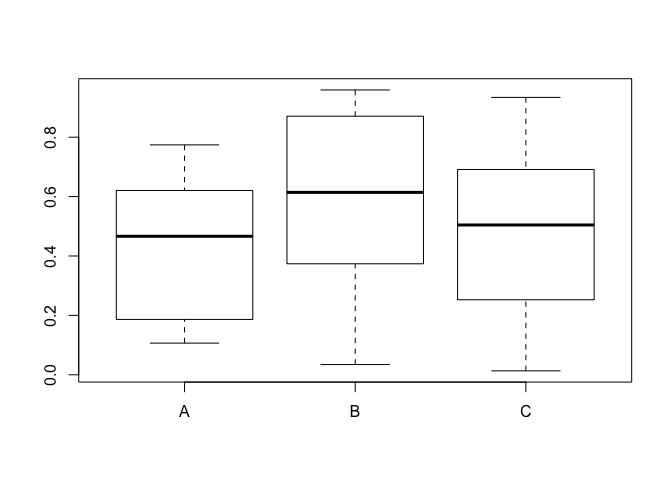
\includegraphics{_main_files/figure-latex/unnamed-chunk-165-1.pdf}

I risultati sono analoghi a quelli che avremmo ottenuto parametrizzando
separatamente le curve per le due varietà ,ma con chiari vantaggi che
illustreremo nel prossimo capitolo.

\section{Confronto tra modelli
alternativi}\label{confronto-tra-modelli-alternativi}

La possibilità di confrontare modelli matematici è forse uno degli
aspetti più rilevanti delle regressioni non-lineari, nel senso che ci
permette di valutare e scegliere ipotesi biologiche, in base alla loro
maggiore o minore compatibilità con le osservazioni sperimentali.

Se prendiamo l'esempio precedente, è rilevante chiedersi se le due
varietà rispondono alla stessa sostanza allelopatica in modo diverso. In
termini statistici abbiamo due modelli alternativi:

\begin{enumerate}
\def\labelenumi{\arabic{enumi}.}
\tightlist
\item
  modello con due curve diverse, una per ogni varietà
\item
  modello alternativo, con un'unica curva di risposta per le due varietà
\end{enumerate}

Questo secondo modello deriva dal primo, semplicemente rimuovendo tre
parametri, cioè un valore di \(b\), uno di \(d\) ed uno di \(e\). Si
tratta quindi di due modelli `nested'. Parametrizziamo il modello
alternativo.

\begin{Shaded}
\begin{Highlighting}[]
\NormalTok{mod.sunR <-}\StringTok{ }\KeywordTok{drm}\NormalTok{(Length }\OperatorTok{~}\StringTok{ }\NormalTok{Dose, }\DataTypeTok{data =}\NormalTok{ sunflower, }\DataTypeTok{fct =} \KeywordTok{LL.3}\NormalTok{())}
\KeywordTok{summary}\NormalTok{(mod.sunR)}
\NormalTok{## }
\NormalTok{## Model fitted: Log-logistic (ED50 as parameter) with lower limit at 0 (3 parms)}
\NormalTok{## }
\NormalTok{## Parameter estimates:}
\NormalTok{## }
\NormalTok{##               Estimate Std. Error t-value   p-value    }
\NormalTok{## b:(Intercept)  3.23478    0.78527  4.1193 0.0004885 ***}
\NormalTok{## d:(Intercept) 76.81273    4.52016 16.9934 9.481e-14 ***}
\NormalTok{## e:(Intercept)  9.46516    0.82245 11.5085 1.568e-10 ***}
\NormalTok{## ---}
\NormalTok{## Signif. codes:  0 '***' 0.001 '**' 0.01 '*' 0.05 '.' 0.1 ' ' 1}
\NormalTok{## }
\NormalTok{## Residual standard error:}
\NormalTok{## }
\NormalTok{##  11.34069 (21 degrees of freedom)}
\end{Highlighting}
\end{Shaded}

Quando i modelli sono `nested' è possibile confrontarli con un test di F
per la `extra sum of squares'. Le devianze del residuo dei due modelli
sono date dalla somma dei quadrati degli scarti: il modello ridotto
presenta, ovviamente, un peggior fitting e quindi una devianza molto più
alta.

\begin{Shaded}
\begin{Highlighting}[]
\NormalTok{devC <-}\StringTok{ }\KeywordTok{sum}\NormalTok{(}\KeywordTok{residuals}\NormalTok{(mod.sun2)}\OperatorTok{^}\DecValTok{2}\NormalTok{)}
\NormalTok{devR <-}\StringTok{ }\KeywordTok{sum}\NormalTok{(}\KeywordTok{residuals}\NormalTok{(mod.sunR)}\OperatorTok{^}\DecValTok{2}\NormalTok{)}
\NormalTok{devC; devR}
\NormalTok{## [1] 1673.388}
\NormalTok{## [1] 2700.837}
\end{Highlighting}
\end{Shaded}

I gradi di libertà delle due devianze sono rispettivamente 24 - 6 = 18
per il modello completo con 6 parametri e 24 - 3 = 21 per il modello
ridotto. La differenza (exra sum of squares) è 1027.448 con 3 gradi di
libertà. Questa quota aggiuntiva è legata alla rimozione dei tre
parametri e la relativa varianza può essere confrontata con la varianza
del residuo del modello completo, per vedere se la rimozione dei
parametri provoca un significativo incremento della mancanza di
adatttamento.

\[ F = \frac{\frac{RSS_c - RSS_s}{df_c - df_s}}{\frac{RSS_c}{df_c}} = \frac{\frac{1027.448}{3}}{\frac{1673.4}{18}}= 3.684\]

A questo valore di F corrisponde una probabilità pari a 0.0315, che ci
permette di rifiutare l'ipotesi nulla di assenza di differenza tra le
due varietà. In R il confronto tra modelli `nested' si esegue con la
funzione anova()

\begin{Shaded}
\begin{Highlighting}[]
\KeywordTok{anova}\NormalTok{(mod.sun2, mod.sunR)}
\NormalTok{## }
\NormalTok{## 1st model}
\NormalTok{##  fct:      LL.3()}
\NormalTok{##  pmodels: 1 (for all parameters)}
\NormalTok{## 2nd model}
\NormalTok{##  fct:      LL.3()}
\NormalTok{##  pmodels: Var (for all parameters)}
\NormalTok{## ANOVA table}
\NormalTok{## }
\NormalTok{##           ModelDf    RSS Df F value p value}
\NormalTok{## 2nd model      21 2700.8                   }
\NormalTok{## 1st model      18 1673.4  3  3.6840  0.0315}
\end{Highlighting}
\end{Shaded}

E'anche possibile confrontare tra di loro i parametri del modello, per
capire quale caratteristica della regressione (pendenza, ED50 o asintoto
superiore) contribuisce maggiormente alla differenza significativa tra
le curve. Questo è possibile con test di t eteroscedastici, nell'ipotesi
che non vi siano correlazioni tra parametri misurati su curve diverse
(il che è vero). Ad esempio, considerando i due ED50 (rispettivamente
11.04 \(\pm\) 1.074 e 8.24 \(\pm\) 0.885), il test di t è:

\[ t = \frac{e_1 - e_2}{\sqrt(ES_1^2 + ES_2^2)} = \frac{11.04 - 8.24}{\sqrt(1.074^2 + 0.885^2)} = 2.012\]

che corrisponde ad una probabilità (due code) P = 0.05956, considerando
un numero di gradi di libertà pari a quelli del residuo. Confronti tra
parametri possono essere compiuti facilmente con la funzione compParm()
in drc.

\begin{Shaded}
\begin{Highlighting}[]
\KeywordTok{compParm}\NormalTok{(mod.sun2, }\DataTypeTok{strVal=}\StringTok{"b"}\NormalTok{, }\DataTypeTok{operator=}\StringTok{"-"}\NormalTok{)}
\NormalTok{## }
\NormalTok{## Comparison of parameter 'b' }
\NormalTok{## }
\NormalTok{##                Estimate Std. Error t-value p-value}
\NormalTok{## Sambro -Oleko  -0.52784    1.46318 -0.3607  0.7225}
\KeywordTok{compParm}\NormalTok{(mod.sun2, }\DataTypeTok{strVal=}\StringTok{"d"}\NormalTok{, }\DataTypeTok{operator=}\StringTok{"-"}\NormalTok{)}
\NormalTok{## }
\NormalTok{## Comparison of parameter 'd' }
\NormalTok{## }
\NormalTok{##                Estimate Std. Error t-value p-value}
\NormalTok{## Sambro -Oleko    4.8704     7.6499  0.6367  0.5324}
\KeywordTok{compParm}\NormalTok{(mod.sun2, }\DataTypeTok{strVal=}\StringTok{"e"}\NormalTok{, }\DataTypeTok{operator=}\StringTok{"-"}\NormalTok{)}
\NormalTok{## }
\NormalTok{## Comparison of parameter 'e' }
\NormalTok{## }
\NormalTok{##                Estimate Std. Error t-value p-value  }
\NormalTok{## Sambro -Oleko    2.7981     1.3915  2.0109 0.05956 .}
\NormalTok{## ---}
\NormalTok{## Signif. codes:  0 '***' 0.001 '**' 0.01 '*' 0.05 '.' 0.1 ' ' 1}
\end{Highlighting}
\end{Shaded}

Vediamo che le due curve sono diverse nel complesso, ma considerando i
singoli parametri, solo \(e\) mostra una differenza vicina alla
significatività.

\subsection{Confronto tra modelli
non-nested}\label{confronto-tra-modelli-non-nested}

Quando le equazioni sono non-nested i confronti non possono essere
effettuati con test statistici formali. In questa situazione si cerca di
utilizzare criteri che tengano conto sia della bontà di adattamento (più
basso è il residuo, migliore è il modello), sia della parsinomia (minore
è il numero dei parametri, migliore è il modello). Un indicatore che
viene spesso utilizzato è l'AKAIKE Information Criterion (AIC):

\[ AIC =  - 2 \, log(2\pi ) + n\,\, log(RSS/n) + n + 2(p + 1) \]

dove RSS è la devianza del residuo, n è il numero di osservazioni e p è
il numero di parametri. Più basso è il valore dell'AIC e migliore è il
modello.

\section{\texorpdfstring{Il package
`drc'}{Il package drc}}\label{il-package-drc}

Abbiamo visto che il package \verb|drc| è estremamente comodo, perchè
contiene tutte le funzioni necessarie per eseguire analisi di
regressione adeguate. Le funzioni disponibili nel pacchetto originale e
nell'estensione collegata a questo libro (con i relativi
\emph{self-starter}) sono

\begin{enumerate}
\def\labelenumi{\arabic{enumi}.}
\tightlist
\item
  log-logistica a due tre e quattro parametri
  (\verb+LL.2(), LL.3(), LL.4()+)
\item
  weibull a due, tre, quattro parametri (\verb+W1.2(), W1.3(), W1.4()+),
\item
  funzione sigmoidale con picco picco iniziale
  (\verb+b3(), b4() e b5()+),
\item
  crescita Gompertz (tre parametrizzazioni alternative:
  \verb+gompGrowth.1()+, \verb+gompGrowth.2()+, \verb+gompGrowth.3()+),
\item
  decrescita esponenziale (\verb+firstOrder()+)
\item
  allometrica (\verb+allometric.1()+), crescita esponenziale
  (\verb+expoGrowth()+), degradazione del primo ordine
  (\verb+firstOrder()+), iperbole rettangolare (\verb+hyperbolic.1()+),
  crescita logistica (tre parametrizzazioni alternative
  \verb+logiGrowth.1(), logiGrowth.2(), logiGrowth.3()+), crescita
  monomolecolare (\verb+monGrowth()+), equazione di Freundlich
  (\verb+DRCpowerCurve()+), loglineare (\verb+DRClogCurve()+),
  esponenziale negativa a due parametri (\verb+DRCnegExp()+),
  regressione asintotica (\verb+DRCasymReg()+), valori estremi
  (\verb+DRCextremeValue()+), funzione di Hill (\verb+DRChill()+),
  Chapman-Richard (\verb+DRCchapman()+).
\end{enumerate}

{[}DA FARE: Come definire una funzione semplice in drm()\ldots{}..{]}

\section{Previsioni}\label{previsioni-1}

In taluni casi, abbastanza frequenti per la verità, l' analisi di
regressione viene eseguita per stimare o predire il valore della Y
corrispondente ad una data X (calibrazione), oppure della X
corrispondente ad un dato Y (esempio determinazione delle dosi
efficaci). Normalmente il problema si riduce alla definizione di
un'equazione predittiva; nel caso della calibrazione essa coincide con
l'equazione originale, nell'altro caso con la sua inversa. Utilizzando
queste equazioni è possibile ottenere il valore cercato e il suo errore
standard, tramite il metodo delta.

Anche da questo punto di vista, drc offre un buon aiuto mediante il
metodo predict(), con il quale possiamo, ad esempio, calcolare la
concentrazione dell'erbicida al tempo 15 (Esempio 1)

\begin{Shaded}
\begin{Highlighting}[]
\KeywordTok{predict}\NormalTok{(modNlin2, }\DataTypeTok{newdata=}\KeywordTok{data.frame}\NormalTok{(}\DataTypeTok{Time=}\DecValTok{15}\NormalTok{), }\DataTypeTok{se.fit=}\OtherTok{TRUE}\NormalTok{)}
\NormalTok{## Prediction }
\NormalTok{##   36.44946}
\end{Highlighting}
\end{Shaded}

Se il modello lo prevede, come nel caso della funzione LL.3(), possiamo
anche ottenere la \ldots{}.

{[}Da completare{]}

\section{Bibliografia}\label{bibliografia}

\chapter*{Appendix 1: breve introduzione ad
R}\label{appendix-1-breve-introduzione-ad-r}
\addcontentsline{toc}{chapter}{Appendix 1: breve introduzione ad R}

\section*{Cosa è R?}\label{cosa-e-r}
\addcontentsline{toc}{section}{Cosa è R?}

R è un software cugino di S-PLUS, con il quale condivide la gran parte
delle procedure ed una perfetta compatibilità. Rispetto al cugino più
famoso, è completamente freeware (sotto la licenza GNU General Public
Licence della Free Software Foundation) ed è nato proprio per mettere a
disposizione degli utenti un software gratuito, potente, mantenendo
comunque la capacità di lavorare in proprio senza usare software di
frodo.

E'uno strumento molto potente, anche da un punto di vista grafico, ma
necessita di una certa pratica, in quanto manca di una vera e propria
interfaccia grafica (Graphical User Interface: GUI) e, di conseguenza, è
spesso necessario scrivere codice.

Inoltre, si tratta di un programma \emph{Open Source}, cioè ognuno può
avere accesso al suo codice interno ed, eventualmente, proporne
modifiche. Altro vantaggio è che, oltre che un programma, R è anche un
linguaggio \emph{object oriented}, che può essere utilizzato dall'utente
per creare funzioni personalizzate.

\textbf{Per evitare noiosi errori che possono essere molto comuni per
chi è abituato a lavorare in ambiente WINDOWS, è bene precisare subito
che R, come tutti i linguaggi di derivazione UNIX, è \emph{case
sensitive}, cioè distingue tra lettere maiuscole e lettere minuscole.}

\section*{Oggetti e assegnazioni}\label{oggetti-e-assegnazioni}
\addcontentsline{toc}{section}{Oggetti e assegnazioni}

\section*{Costanti e vettori}\label{costanti-e-vettori}
\addcontentsline{toc}{section}{Costanti e vettori}

R lavora con valori, stringhe di caratteri, vettori e matrici, che
vengono assegnati alle variabili con opportuni comandi. Ad esempio, il
comando:

\begin{Shaded}
\begin{Highlighting}[]
\NormalTok{y  <-}\StringTok{  }\DecValTok{3}
\NormalTok{y}
\NormalTok{## [1] 3}
\end{Highlighting}
\end{Shaded}

assegna il valore 3 alla variabile \emph{y}. Invece il comando:

\begin{Shaded}
\begin{Highlighting}[]
\NormalTok{x  <-}\StringTok{  }\KeywordTok{c}\NormalTok{(}\DecValTok{1}\NormalTok{, }\DecValTok{2}\NormalTok{, }\DecValTok{3}\NormalTok{)}
\NormalTok{x}
\NormalTok{## [1] 1 2 3}
\end{Highlighting}
\end{Shaded}

crea un vettore \emph{x} contenente i numeri 1,2 e 3. Bisogna precisare
che il `vettore', in R, non ha alcun legame con la fisica o l'algebra,
ed è semplicemente una collezione di numeri (o strighe) consecutivi.

\section*{Matrici}\label{matrici}
\addcontentsline{toc}{section}{Matrici}

Oltre ai vettori, in R possiamo definire le matrici. Ad esempio il
comando:

\begin{Shaded}
\begin{Highlighting}[]
\NormalTok{z  <-}\StringTok{  }\KeywordTok{matrix}\NormalTok{(}\KeywordTok{c}\NormalTok{(}\DecValTok{1}\NormalTok{, }\DecValTok{2}\NormalTok{, }\DecValTok{3}\NormalTok{, }\DecValTok{4}\NormalTok{, }\DecValTok{5}\NormalTok{, }\DecValTok{6}\NormalTok{, }\DecValTok{7}\NormalTok{, }\DecValTok{8}\NormalTok{), }\DecValTok{2}\NormalTok{, }\DecValTok{4}\NormalTok{, }\DataTypeTok{byrow=}\OtherTok{TRUE}\NormalTok{)}
\end{Highlighting}
\end{Shaded}

crea una matrice \emph{z} a 2 righe e 4 colonne, contenente i numeri da
1 a 8. La matrice viene riempita per riga.

Come già mostrato, per visualizzare il contenuto di una variabile basta
digitare il nome della variabile. Ad esempio:

\begin{Shaded}
\begin{Highlighting}[]
\NormalTok{z}
\NormalTok{##      [,1] [,2] [,3] [,4]}
\NormalTok{## [1,]    1    2    3    4}
\NormalTok{## [2,]    5    6    7    8}
\end{Highlighting}
\end{Shaded}

Gli elementi di una matrice possono essere richiamati con un opportuno
utilizzo delle parentesi quadre:

\begin{Shaded}
\begin{Highlighting}[]
\NormalTok{z[}\DecValTok{1}\NormalTok{,}\DecValTok{3}\NormalTok{]}
\NormalTok{## [1] 3}
\end{Highlighting}
\end{Shaded}

\section*{Operazioni ed operatori}\label{operazioni-ed-operatori}
\addcontentsline{toc}{section}{Operazioni ed operatori}

Le variabili possono essere create anche con opportune operazioni
algebriche, che si eseguono utilizzando i normali operatori (+, -, *,
/). Ad esempio:

\begin{Shaded}
\begin{Highlighting}[]
\NormalTok{f  <-}\StringTok{  }\DecValTok{2} \OperatorTok{*}\StringTok{ }\NormalTok{y}
\NormalTok{f}
\NormalTok{## [1] 6}
\end{Highlighting}
\end{Shaded}

\section*{Funzioni ed argomenti}\label{funzioni-ed-argomenti}
\addcontentsline{toc}{section}{Funzioni ed argomenti}

Per eseguire operazioni particolari si utilizzano, in genere, le
funzioni. Una funzione è richiamata con un nome ed uno o più argomenti.
Ad esempio, il comando:

\begin{Shaded}
\begin{Highlighting}[]
\KeywordTok{log}\NormalTok{(}\DecValTok{5}\NormalTok{)}
\NormalTok{## [1] 1.609438}
\end{Highlighting}
\end{Shaded}

Calcola il logaritmo naturale di 5 e richiede un solo argomento, cioè il
numero di cui calcolare il logaritmo. Al contrario, il comando:

\begin{Shaded}
\begin{Highlighting}[]
\KeywordTok{log}\NormalTok{(}\DecValTok{100}\NormalTok{, }\DecValTok{2}\NormalTok{)}
\NormalTok{## [1] 6.643856}
\end{Highlighting}
\end{Shaded}

Calcola il logaritmo in base 2 di 100 e richiede due argomenti, cioè il
numero di cui calcolare il logaritmo e la base del logaritmo. Quando
sono necessari due o più argomenti essi debbono essere messi nell'ordine
esatto (in questo caso prima il numero poi la base) oppure debbono
essere utilizzati i riferimenti corretti. Ad esempio, i due comandi:

\begin{Shaded}
\begin{Highlighting}[]
\KeywordTok{log}\NormalTok{(}\DecValTok{100}\NormalTok{, }\DataTypeTok{base=}\DecValTok{2}\NormalTok{)}
\NormalTok{## [1] 6.643856}
\KeywordTok{log}\NormalTok{(}\DataTypeTok{base=}\DecValTok{2}\NormalTok{, }\DecValTok{100}\NormalTok{)}
\NormalTok{## [1] 6.643856}
\end{Highlighting}
\end{Shaded}

restituiscono lo stesso risultato, al contrario dei due comandi
seguenti:

\begin{Shaded}
\begin{Highlighting}[]
\KeywordTok{log}\NormalTok{(}\DecValTok{100}\NormalTok{, }\DecValTok{2}\NormalTok{)}
\NormalTok{## [1] 6.643856}
\KeywordTok{log}\NormalTok{(}\DecValTok{2}\NormalTok{, }\DecValTok{100}\NormalTok{)}
\NormalTok{## [1] 0.150515}
\end{Highlighting}
\end{Shaded}

\section*{Dataframe}\label{dataframe}
\addcontentsline{toc}{section}{Dataframe}

Oltre a vettori e matrici, in R esiste un altro importante oggetto, cioè
il \emph{dataframe}, costituito da una tabella di dati con una o più
colonne di variabili e una o più righe di dati. A differenza della
matrice, il dataframe può essere utilizzato per memorizzare variabili di
diverso tipo (numeri e caratteri). Un dataframe può essere creato unendo
più vettori, come nell'esempio seguente.

\begin{Shaded}
\begin{Highlighting}[]
\NormalTok{parcelle  <-}\StringTok{  }\KeywordTok{c}\NormalTok{(}\DecValTok{1}\NormalTok{, }\DecValTok{2}\NormalTok{, }\DecValTok{3}\NormalTok{, }\DecValTok{4}\NormalTok{, }\DecValTok{5}\NormalTok{, }\DecValTok{6}\NormalTok{)}
\NormalTok{tesi  <-}\StringTok{  }\KeywordTok{factor}\NormalTok{(}\KeywordTok{c}\NormalTok{(}\StringTok{"A"}\NormalTok{, }\StringTok{"A"}\NormalTok{, }\StringTok{"B"}\NormalTok{, }\StringTok{"B"}\NormalTok{, }\StringTok{"C"}\NormalTok{, }\StringTok{"C"}\NormalTok{))}
\NormalTok{dati  <-}\StringTok{  }\KeywordTok{c}\NormalTok{(}\DecValTok{12}\NormalTok{, }\DecValTok{15}\NormalTok{, }\DecValTok{16}\NormalTok{, }\DecValTok{13}\NormalTok{, }\DecValTok{11}\NormalTok{, }\DecValTok{19}\NormalTok{)}
\NormalTok{tabella  <-}\StringTok{  }\KeywordTok{data.frame}\NormalTok{(}\StringTok{"Parc"}\NormalTok{=parcelle,}\StringTok{"Tesi"}\NormalTok{=tesi,}\StringTok{"Produzioni"}\NormalTok{=dati)}
\NormalTok{tabella}
\NormalTok{##   Parc Tesi Produzioni}
\NormalTok{## 1    1    A         12}
\NormalTok{## 2    2    A         15}
\NormalTok{## 3    3    B         16}
\NormalTok{## 4    4    B         13}
\NormalTok{## 5    5    C         11}
\NormalTok{## 6    6    C         19}
\end{Highlighting}
\end{Shaded}

Per utilizzare i dati in un dataframe, bisognerà accedere ai singoli
vettori colonna che lo costituiscono. Per far questo possiamo utilizzare
l'estrattore \emph{\$}:

\begin{Shaded}
\begin{Highlighting}[]
\NormalTok{tabella}\OperatorTok{$}\NormalTok{Parc}
\NormalTok{## [1] 1 2 3 4 5 6}
\end{Highlighting}
\end{Shaded}

oppure possiamo utilizzare gli indici, che nel caso del dataframe, cioè
una struttura dati bidimensionale, sono due, uno per le righe e uno per
le colonne, separati da virgole:

\begin{Shaded}
\begin{Highlighting}[]
\NormalTok{tabella[,}\DecValTok{1}\NormalTok{]}
\NormalTok{## [1] 1 2 3 4 5 6}
\end{Highlighting}
\end{Shaded}

oppure si può usare il comando \emph{attach()}, che crea immediatamente
tre vettori (Pianta, Varietà e Altezza), disponibili per le successive
elaborazioni.Possiamo osservare infatti che, dopo aver creato la matrice
`tabella', digitando quanto segue R ci mette a disposizione il vettore
`Produzioni'.

\begin{Shaded}
\begin{Highlighting}[]
\KeywordTok{attach}\NormalTok{(tabella)}
\NormalTok{## The following objects are masked from tabella (pos = 3):}
\NormalTok{## }
\NormalTok{##     Parc, Produzioni, Tesi}
\NormalTok{## The following objects are masked from tabella (pos = 4):}
\NormalTok{## }
\NormalTok{##     Parc, Produzioni, Tesi}
\NormalTok{## The following objects are masked from tabella (pos = 6):}
\NormalTok{## }
\NormalTok{##     Parc, Produzioni, Tesi}
\NormalTok{Produzioni}
\NormalTok{## [1] 12 15 16 13 11 19}
\end{Highlighting}
\end{Shaded}

I dataframe possono essere editati velocemente utilizzando il comando
\emph{fix}, che fa apparire una finestra di editing tipo `foglio
elettronico'.

\section*{Quale oggetto sto
utilizzando?}\label{quale-oggetto-sto-utilizzando}
\addcontentsline{toc}{section}{Quale oggetto sto utilizzando?}

Per avere informazioni sulla natura di un oggetto creato in R, posso
usare la funzione \texttt{str()}, come nell'esempio seguente:

\begin{Shaded}
\begin{Highlighting}[]
\KeywordTok{str}\NormalTok{(tabella)}
\NormalTok{## 'data.frame':    6 obs. of  3 variables:}
\NormalTok{##  $ Parc      : num  1 2 3 4 5 6}
\NormalTok{##  $ Tesi      : Factor w/ 3 levels "A","B","C": 1 1 2 2 3 3}
\NormalTok{##  $ Produzioni: num  12 15 16 13 11 19}
\end{Highlighting}
\end{Shaded}

Vediamo infatti che R ci informa che l'oggetto `tabella' è in realtà un
dataframe composto da tre colonne, di cui la prima e la terza sono
numeriche, mentre la seconda è una variabile qualitativa (fattore).

\section*{Consigli per l'immissione di dati
sperimentali}\label{consigli-per-limmissione-di-dati-sperimentali}
\addcontentsline{toc}{section}{Consigli per l'immissione di dati
sperimentali}

I dati delle prove sperimentali si possono o importare in R da altri
software (ad esempio Excel) oppue si possono digitare direttamente in R.
In quest'ultimo caso, in genere, si crea un vettore per ogni colonna di
dati e, successivamente, si riuniscono i vettori in un dataframe, che
viene poi salvato nel workspace, come vedremo in seguito.

\subsection*{Immissione manuale di
dati}\label{immissione-manuale-di-dati}
\addcontentsline{toc}{subsection}{Immissione manuale di dati}

L'immissione dei dati in R (e quindi la creazione di vettori) può essere
velocizzata utilizzando la funzione \texttt{scan()}, separando i dati
con INVIO (questo è comodo perchè ci permette di lavorare senza
abbandonare il tastierino numerico!). L'immissione termina quando si
digita un INVIO a vuoto.

\begin{verbatim}
dati <- scan()
1: 12
2: 14
3: 16
4: 18
5: 20
6:
Read 5 items
dati
[1] 12 14 16 18 20
\end{verbatim}

La stessa funzione può essere anche utilizzata per immettere comodamente
stringhe di caratteri, con un opportuno impiego dell'argomento
\texttt{what}. In questo caso è possibile omettere le virgolette.

\begin{verbatim}
tesi  <-  scan(what = "character")
1: aurelio
2: aurelio
3: aurelio
4: claudio
5: claudio
6: claudio
7: latino
8: latino
9: latino
10: 
Read 9 items
tesi
[1] "aurelio" "aurelio" "aurelio" "claudio" 
    "claudio" "claudio" "latino"  "latino"  "latino" 
>
\end{verbatim}

\subsection*{Immissione di numeri
progressivi}\label{immissione-di-numeri-progressivi}
\addcontentsline{toc}{subsection}{Immissione di numeri progressivi}

Per creare una serie progressiva, si può utilizzare il comando
\texttt{seq(n,m,by=step)} che genera una sequenza da \(n\) a \(m\) con
passo pari a \(step\).

\begin{Shaded}
\begin{Highlighting}[]
\NormalTok{parcelle  <-}\StringTok{  }\KeywordTok{seq}\NormalTok{(}\DecValTok{1}\NormalTok{,}\DecValTok{50}\NormalTok{,}\DecValTok{1}\NormalTok{)}
\NormalTok{parcelle}
\NormalTok{##  [1]  1  2  3  4  5  6  7  8  9 10 11 12 13 14 15 16 17 18 19 20 21 22 23}
\NormalTok{## [24] 24 25 26 27 28 29 30 31 32 33 34 35 36 37 38 39 40 41 42 43 44 45 46}
\NormalTok{## [47] 47 48 49 50}
\end{Highlighting}
\end{Shaded}

\subsection*{Immissione dei codici delle tesi e dei
blocchi}\label{immissione-dei-codici-delle-tesi-e-dei-blocchi}
\addcontentsline{toc}{subsection}{Immissione dei codici delle tesi e dei
blocchi}

A volte i codici delle tesi sono sequenze ripetute di stringhe. Ad
esempio, i primi quattro dati potrebbero essere riferiti alla varietà
BAIO, i secondi quattro alla varietà DUILIO, i successivi quattro alla
varietà PLINIO. Per creare velocemente questo vettore, possiamo
utilizzare la funzione \texttt{rep()}, in questo modo.

\begin{Shaded}
\begin{Highlighting}[]
\NormalTok{tesi  <-}\StringTok{  }\KeywordTok{factor}\NormalTok{(}\KeywordTok{c}\NormalTok{(}\StringTok{"BAIO"}\NormalTok{, }\StringTok{"DUILIO"}\NormalTok{, }\StringTok{"PLINIO"}\NormalTok{))}
\NormalTok{tesi}
\NormalTok{## [1] BAIO   DUILIO PLINIO}
\NormalTok{## Levels: BAIO DUILIO PLINIO}
\NormalTok{tesi  <-}\StringTok{  }\KeywordTok{rep}\NormalTok{(tesi,}\DataTypeTok{each=}\DecValTok{4}\NormalTok{)}
\NormalTok{tesi}
\NormalTok{##  [1] BAIO   BAIO   BAIO   BAIO   DUILIO DUILIO DUILIO DUILIO PLINIO PLINIO}
\NormalTok{## [11] PLINIO PLINIO}
\NormalTok{## Levels: BAIO DUILIO PLINIO}
\end{Highlighting}
\end{Shaded}

Notare l'uso della funzione \texttt{factor()} per creare un vettore di
dati qualitativi (fattore). Allo stesso modo, per immettere i codici dei
blocchi possiamo utilizzare la stessa funzione in un modo diverso.
Ammettiamo infatti che i quattro valori di ogni tesi appartengano
rispettivamente ai quattro blocchi; si opera quindi in questo modo.

\begin{Shaded}
\begin{Highlighting}[]
\NormalTok{tesi  <-}\StringTok{  }\NormalTok{(}\KeywordTok{c}\NormalTok{ (}\DecValTok{1}\NormalTok{, }\DecValTok{2}\NormalTok{, }\DecValTok{3}\NormalTok{, }\DecValTok{4}\NormalTok{))}
\NormalTok{tesi <-}\StringTok{ }\KeywordTok{rep}\NormalTok{(tesi, }\DataTypeTok{times=}\DecValTok{3}\NormalTok{)}
\NormalTok{tesi}
\NormalTok{##  [1] 1 2 3 4 1 2 3 4 1 2 3 4}
\end{Highlighting}
\end{Shaded}

\subsection*{Leggere e salvare dati
esterni}\label{leggere-e-salvare-dati-esterni}
\addcontentsline{toc}{subsection}{Leggere e salvare dati esterni}

Oltre che immessi da tastiera, i dati possono essere importati in R da
files esterni, Inoltre, gli oggetti di R creati nel corso di una
sessione possono essere memorizzati su files esterni. Partiamo dal
presupposto di aver creato (come frequentemente avviene) il nostro
database con EXCEL e di volerlo importare in R nel DATAFRAME
\emph{dati}.

Creiamo in EXCEL la tabella riportata di seguito, che si riferisce a 20
piante di mais.

\begin{longtable}[]{@{}lll@{}}
\toprule
Pianta & Var & Altezza\tabularnewline
\midrule
\endhead
1 & N & 172\tabularnewline
2 & S & 154\tabularnewline
3 & V & 150\tabularnewline
4 & V & 188\tabularnewline
5 & C & 162\tabularnewline
6 & N & 145\tabularnewline
7 & C & 157\tabularnewline
8 & C & 178\tabularnewline
9 & V & 175\tabularnewline
10 & N & 158\tabularnewline
11 & N & 153\tabularnewline
12 & N & 191\tabularnewline
13 & S & 174\tabularnewline
14 & C & 141\tabularnewline
15 & N & 165\tabularnewline
16 & C & 163\tabularnewline
17 & V & 148\tabularnewline
18 & S & 152\tabularnewline
19 & C & 169\tabularnewline
20 & C & 185\tabularnewline
\bottomrule
\end{longtable}

La procedura è la seguente:

\begin{enumerate}
\def\labelenumi{\arabic{enumi}.}
\tightlist
\item
  salviamo questa tabella nel file di testo: \emph{comma delineated}
  `import.csv'. Per far questo scegliere `Menù - File - Salva con nome'.
  Scegliere un nome per il file ed indicare: 'Tipo file = CSV
  (delimitato dal separatore di elenco) (*.csv). Salvare quindi il file
  in una directory prescelta.
\item
  Avviare una sessione R, cambiare la directory predefinita del sistema,
  scegliendo, con il menu File - Change Directory, la cartella nella
  quale abbiamo memorizzato il file di importazione.
\item
  Leggere il file di testo in un dataframe, con il seguente comando:
\end{enumerate}

\begin{verbatim}
setwd("myWorkingDir")
dati  <-  read.csv("import.csv", header=TRUE)
\end{verbatim}

Il comando appena descritto ha successo per file CSV creati con la
versione inglese di Windows, caratterizzati dal punto come separatore
decimale e dalla virgola come separatore di elenco. Se invece il
computer fosse settato all'italiana, con la virgola come separatore
decimale e il punto e virgola come separatore di elenco, allora si
potrebbe utilizzare la funzione \texttt{read.csv2()} (stessa sintassi).
Con questi due comandi, in R viene creato un dataframe di nome dati,
contenente le tre colonne della tabella `import.csv' appena creata,
comprese le intestazioni di colonna.

I dati contenuti in un dataframe o in qualunque altro oggetto possono
essere salvati in un file esterno (in formato R binario):

\begin{verbatim}
save(file="dati1.rda", dati)
\end{verbatim}

ed eventualmente ricaricati:

\begin{verbatim}
load("dati1.rda")
\end{verbatim}

Per scrivere in un file di testo (in questo caso \emph{comma
delineated}, ma il separatore di elenco può essere modificato secondo le
nostre esigenze con l'argomento \texttt{sep}) si utilizza il seguente
comando:

\begin{verbatim}
write.table(dati, "residui.csv", row.names=FALSE, 
              col.names=TRUE, sep=",")
\end{verbatim}

\section*{Alcune operazioni comuni sul
dataset}\label{alcune-operazioni-comuni-sul-dataset}
\addcontentsline{toc}{section}{Alcune operazioni comuni sul dataset}

\subsection*{Selezionare un subset di
dati}\label{selezionare-un-subset-di-dati}
\addcontentsline{toc}{subsection}{Selezionare un subset di dati}

E' possibile estrarre da un dataframe un subset di dati utilizzando la
funzione:

\begin{verbatim}
subset(dataframe, condizione)
\end{verbatim}

Ad esempio, se consideriamo il dataframe tabella creato in precedenza, è
possibile selezionare tutte le righe relative alle Tesi A e C come
segue:

\begin{Shaded}
\begin{Highlighting}[]
\NormalTok{tabella2  <-}\StringTok{  }\KeywordTok{subset}\NormalTok{(tabella, Tesi }\OperatorTok{==}\StringTok{ "A"} \OperatorTok{|}\StringTok{ }\NormalTok{Tesi }\OperatorTok{==}\StringTok{ "C"}\NormalTok{)}
\NormalTok{tabella2}
\NormalTok{##   Parc Tesi Produzioni}
\NormalTok{## 1    1    A         12}
\NormalTok{## 2    2    A         15}
\NormalTok{## 5    5    C         11}
\NormalTok{## 6    6    C         19}
\end{Highlighting}
\end{Shaded}

Notare il carattere ``\textbar{}'' che esprime la condizione logica OR.
La condizione logica AND si esprime con il carattere ``\&''. L'esempio
seguente isola i record in cui le varietà sono A o C e,
contemporaneamente, la produzione è minore di 19.

\begin{Shaded}
\begin{Highlighting}[]
\NormalTok{tabella3  <-}\StringTok{  }\KeywordTok{subset}\NormalTok{(tabella, Tesi }\OperatorTok{==}\StringTok{ "A"} \OperatorTok{|}\StringTok{ }\NormalTok{Tesi }\OperatorTok{==}\StringTok{ "C"} \OperatorTok{&}\StringTok{ }
\StringTok{                       }\NormalTok{Produzioni }\OperatorTok{<}\StringTok{ }\DecValTok{19}\NormalTok{)}
\NormalTok{tabella3}
\NormalTok{##   Parc Tesi Produzioni}
\NormalTok{## 1    1    A         12}
\NormalTok{## 2    2    A         15}
\NormalTok{## 5    5    C         11}
\end{Highlighting}
\end{Shaded}

\subsection*{Ordinare un vettore o un
dataframe}\label{ordinare-un-vettore-o-un-dataframe}
\addcontentsline{toc}{subsection}{Ordinare un vettore o un dataframe}

Un vettore (numerico o carattere) può essere ordinato con il comando
\texttt{sort}:

\begin{Shaded}
\begin{Highlighting}[]
\NormalTok{y  <-}\StringTok{  }\KeywordTok{c}\NormalTok{(}\DecValTok{12}\NormalTok{, }\DecValTok{15}\NormalTok{, }\DecValTok{11}\NormalTok{, }\DecValTok{17}\NormalTok{, }\DecValTok{12}\NormalTok{, }\DecValTok{8}\NormalTok{, }\DecValTok{7}\NormalTok{, }\DecValTok{15}\NormalTok{)}
\KeywordTok{sort}\NormalTok{(y, }\DataTypeTok{decreasing =} \OtherTok{FALSE}\NormalTok{)}
\NormalTok{## [1]  7  8 11 12 12 15 15 17}
\NormalTok{z  <-}\StringTok{  }\KeywordTok{c}\NormalTok{(}\StringTok{"A"}\NormalTok{, }\StringTok{"C"}\NormalTok{, }\StringTok{"D"}\NormalTok{, }\StringTok{"B"}\NormalTok{, }\StringTok{"F"}\NormalTok{, }\StringTok{"L"}\NormalTok{, }\StringTok{"M"}\NormalTok{, }\StringTok{"E"}\NormalTok{)}
\KeywordTok{sort}\NormalTok{(z, }\DataTypeTok{decreasing =} \OtherTok{TRUE}\NormalTok{)}
\NormalTok{## [1] "M" "L" "F" "E" "D" "C" "B" "A"}
\end{Highlighting}
\end{Shaded}

Un dataframe può essere invece ordinato con il comando \texttt{order()},
facendo attenzione al segno meno utilizzabile per l'ordinamento
decrescente.

\begin{verbatim}
dataset[order(dataset$z, dataset$y), ]
dataset[order(dataset$z, -dataset$y), ]
\end{verbatim}

\section*{Workspace}\label{workspace}
\addcontentsline{toc}{section}{Workspace}

Gli oggetti creati durante una sessione di lavoro vengono memorizzati
nel cosiddetto workspace. Per il salvataggio del workspace nella
directory corrente si usa il menu (File/Save Workspace) oppure il
comando:

\begin{verbatim}
save.image('nomefile.RData')
\end{verbatim}

Il contenuto del workspace viene visualizzato con:

\begin{verbatim}
ls()
\end{verbatim}

Il workspace viene richiamato da menu (File/Open Workspace) oppure con
il comando:

\begin{verbatim}
load('nomefile.RData')
\end{verbatim}

Per un lavoro efficiente in R è bene tenere il workspace molto pulito,
eliminando gli oggetti non necessari. La completa eliminazione degli
oggetti nel workspace si esegue con:

\begin{verbatim}
rm(list=ls())
\end{verbatim}

Uno o più oggetti specifici possono essere eliminati con:

\begin{verbatim}
rm(oggetto1, oggetto2, .....)
\end{verbatim}

Gli oggetti possono anche essere richiamati in base alla loro posizione;
ad esempio il comando:

\begin{verbatim}
rm(list=ls()[3:4])
\end{verbatim}

elimina il terzo e il quarto oggetto dal workspace.

Un comando particolarmente utile è il seguente:

\begin{verbatim}
rm(list=ls()[ls()!="oggetto1"])
\end{verbatim}

che permette di eliminare dal workspace ogni oggetto meno ``oggetto1''.
Si possono utilizzare anche clausole logiche più articolate come la
seguente:

\begin{verbatim}
rm(list=ls()[ls()!="oggetto1" & ls()!="oggetto2"])
\end{verbatim}

che elimina tutto meno ``oggetto1'' e ``oggetto2''.

\section*{Script o programmi}\label{script-o-programmi}
\addcontentsline{toc}{section}{Script o programmi}

Come è possibile memorizzare dati e workspace, è anche possibile creare
uno script (procedura, funzione\ldots{}) da memorizzare e richiamare in
seguito. Nel caso più semplice è possibile scrivere comandi in un
semplice editor di testo e salvarli in un file con estensione `.r'. I
comandi possono poi essere riutilizzati per semplice copia ed incolla
sulla console, opppure, nel caso in cui si utilizzi Rstudio (FILE -\(>\)
APRI SCRIPT o NUOVO SCRIPT) selezionando il comando (o i comandi) da
inviare alla console e premendo la combinazione CTRL + INVIO.

Lavorare con scripts è molto comodo e consigliabile perchè non si deve
partire da zero ad ogni sessione, ma è sufficiente correggere i comandi
digitati in sessioni precedenti.

Oltre agli script, è possibile creare funzioni personalizzate fino ad
arrivare a veri e propri programmi (packages). Immaginiamo ad esempio di
voler scrivere una funzione che, dato il valore della produzione
rilevata in una parcella di orzo di 20 \$ m\^{}2 \$ (in kg) e la sua
umidità percentuale, calcoli automaticamente il valore della produzione
secca in kg/ha. La funzione che dobbiamo implementare è:

\[
PS = PU \cdot \frac{100 - U}{100} \cdot \frac{10000}{20}
\]

ove PS è la produzione secca in kg/ha e PU è la produzione all'umidità U
in kg per 20 \$ m\^{}2 \$.

Scriveremo un file di testo (ad esempio con il \emph{Block notes} o con
l'editor interno ad R):

\begin{verbatim}
PS  <-  function(PU, U) {
  PU*((100-U)/100)*(10000/20)
}
\end{verbatim}

Notare l'uso delle parentesi graffe. Salveremo il file di testo con il
nome (ad esempio) ``prova.r''.

Aprendo una nuova sessione in R, possiamo ricaricare in memoria il file
di programma (FILE - SORGENTE CODICE R, oppure da console, con il
comando:

\begin{verbatim}
source('prova.r')
\end{verbatim}

A differenza di quanto avviene con uno script, i comandi memorizzati
nella funzione non vengono eseguiti, ma la funzione `PS' diviene
disponibile nel workspace e può essere utilizzata nel modo seguente:

\begin{verbatim}
PS(20,85)
\end{verbatim}

\section*{Interrogazione di oggetti}\label{interrogazione-di-oggetti}
\addcontentsline{toc}{section}{Interrogazione di oggetti}

A differenza di altri linguaggi statistici come SAS o SPSS, R
immagazzina i risultati delle analisi negli oggetti, mostrando un output
video piuttosto minimale. Per ottenere informazioni è necessario
interrogare opportunamente gli oggetti che al loro interno possono
contenere altri oggetti da cui recuperare le informazioni interessanti.
Gli oggetti che contengono altri oggetti sono detti \textbf{liste}.

Ad esempio, se vogliamo calcolare autovettori ed autovalori di una
matrice, utilizziamo la funzione `eigen'. Questa funzione restituisce
una lista di oggetti, che al suo interno contiene i due oggetti values
(autovalori) e vectors (autovettori). Per recuperare l'uno o l'altro dei
due risultati (autovettori o autovalori) si usa l'operatore di
concatenamento (detto anche estrattore) \$.

\begin{Shaded}
\begin{Highlighting}[]
\NormalTok{matrice  <-}\StringTok{  }\KeywordTok{matrix}\NormalTok{(}\KeywordTok{c}\NormalTok{(}\DecValTok{2}\NormalTok{,}\DecValTok{1}\NormalTok{,}\DecValTok{3}\NormalTok{,}\DecValTok{4}\NormalTok{),}\DecValTok{2}\NormalTok{,}\DecValTok{2}\NormalTok{)}
\NormalTok{matrice}
\NormalTok{##      [,1] [,2]}
\NormalTok{## [1,]    2    3}
\NormalTok{## [2,]    1    4}
\NormalTok{ev  <-}\StringTok{  }\KeywordTok{eigen}\NormalTok{(matrice)}
\NormalTok{ev}
\NormalTok{## eigen() decomposition}
\NormalTok{## $values}
\NormalTok{## [1] 5 1}
\NormalTok{## }
\NormalTok{## $vectors}
\NormalTok{##            [,1]       [,2]}
\NormalTok{## [1,] -0.7071068 -0.9486833}
\NormalTok{## [2,] -0.7071068  0.3162278}
\NormalTok{ev}\OperatorTok{$}\NormalTok{values}
\NormalTok{## [1] 5 1}
\NormalTok{ev}\OperatorTok{$}\NormalTok{vectors}
\NormalTok{##            [,1]       [,2]}
\NormalTok{## [1,] -0.7071068 -0.9486833}
\NormalTok{## [2,] -0.7071068  0.3162278}
\end{Highlighting}
\end{Shaded}

\section*{Altre funzioni matriciali}\label{altre-funzioni-matriciali}
\addcontentsline{toc}{section}{Altre funzioni matriciali}

Oltre che autovettori ed autovalori di una matrice, R ci permette di
gestire altre funzioni di matrice. Se ad esempio abbiamo le matrici:

\[
Z = \left( {\begin{array}{*{20}c}
   1 & 2  
   2 & 3  
\end{array}} \right)\,\,\,\,\,\,\,Y = \left( {\begin{array}{*{20}c}
   3 & 2  
\end{array}} \right)
\]

queste possono essere caricate in R con i seguenti comandi:

\begin{Shaded}
\begin{Highlighting}[]
\NormalTok{Z  <-}\StringTok{  }\KeywordTok{matrix}\NormalTok{(}\KeywordTok{c}\NormalTok{(}\DecValTok{1}\NormalTok{,}\DecValTok{2}\NormalTok{,}\DecValTok{2}\NormalTok{,}\DecValTok{3}\NormalTok{),}\DecValTok{2}\NormalTok{,}\DecValTok{2}\NormalTok{)}
\NormalTok{Y  <-}\StringTok{  }\KeywordTok{matrix}\NormalTok{(}\KeywordTok{c}\NormalTok{(}\DecValTok{3}\NormalTok{,}\DecValTok{2}\NormalTok{),}\DecValTok{1}\NormalTok{,}\DecValTok{2}\NormalTok{)}
\end{Highlighting}
\end{Shaded}

Possiamo poi ottenere la trasposta di Z con il comando:

\begin{Shaded}
\begin{Highlighting}[]
\KeywordTok{t}\NormalTok{(Z)}
\NormalTok{##      [,1] [,2]}
\NormalTok{## [1,]    1    2}
\NormalTok{## [2,]    2    3}
\end{Highlighting}
\end{Shaded}

Possiamo moltiplicare Y e Z utilizzando l'operatore \%*\%:

\begin{Shaded}
\begin{Highlighting}[]
\NormalTok{Y}\OperatorTok\NormalTok{Z}
\NormalTok{##      [,1] [,2]}
\NormalTok{## [1,]    7   12}
\end{Highlighting}
\end{Shaded}

Possiamo calcolare l'inversa di Z con:

\begin{Shaded}
\begin{Highlighting}[]
\KeywordTok{solve}\NormalTok{(Z)}
\NormalTok{##      [,1] [,2]}
\NormalTok{## [1,]   -3    2}
\NormalTok{## [2,]    2   -1}
\end{Highlighting}
\end{Shaded}

\section*{Cenni sulle funzionalità grafiche in
R}\label{cenni-sulle-funzionalita-grafiche-in-r}
\addcontentsline{toc}{section}{Cenni sulle funzionalità grafiche in R}

R è un linguaggio abbastanza potente e permette di creare grafici
interessanti. Ovviamente un trattazione esauriente esula dagli scopi di
questo testo, anche se è opportuno dare alcune indicazioni che
potrebbero essere utili in seguito. La funzione più utilizzata per
produrre grafici è:

\begin{verbatim}
plot(x,y, type, xlab, ylab, col, lwd, lty...)
\end{verbatim}

ovex ed y sono i vettori con le coordinate dei punti da disegnare.
\texttt{Type} rappresenta il tipo di grafico (`'p'`produce un grafico a
punti,'`l'`un grafico a linee,'`b'`disegna punti uniti da linee,'`h''
disegna istogrammi), 'Title disegna il titolo del grafico, sub il
sottotitolo,xlab e ylab le etichette degli assi, col è il colore
dell'oggetto, lwd il suo spessore, lty il tipo di linea e cos'i via.

Per una descrizione più dettagliata si consiglia di consultare la
documentazione on line. A titolo di esempio mostriamo l'output dei
comandi:

\begin{Shaded}
\begin{Highlighting}[]
\NormalTok{x  <-}\StringTok{  }\KeywordTok{c}\NormalTok{(}\DecValTok{1}\NormalTok{,}\DecValTok{2}\NormalTok{,}\DecValTok{3}\NormalTok{,}\DecValTok{4}\NormalTok{)}
\NormalTok{y  <-}\StringTok{  }\KeywordTok{c}\NormalTok{(}\DecValTok{10}\NormalTok{,}\DecValTok{11}\NormalTok{,}\DecValTok{13}\NormalTok{,}\DecValTok{17}\NormalTok{)}
\KeywordTok{plot}\NormalTok{(x, y, }\StringTok{"p"}\NormalTok{, }\DataTypeTok{col=}\StringTok{"red"}\NormalTok{, }\DataTypeTok{lwd=}\DecValTok{5}\NormalTok{,}\DataTypeTok{xlab=}\StringTok{"Ascissa"}\NormalTok{, }\DataTypeTok{ylab=}\StringTok{"Ordinata"}\NormalTok{)}
\end{Highlighting}
\end{Shaded}

\includegraphics{_main_files/figure-latex/unnamed-chunk-197-1.pdf}

Per sovrapporre un'altra serie di punti alla precedente possiamo
utilizzare il comando `points':

\begin{Shaded}
\begin{Highlighting}[]
\NormalTok{y2  <-}\StringTok{  }\KeywordTok{c}\NormalTok{(}\DecValTok{17}\NormalTok{,}\DecValTok{13}\NormalTok{,}\DecValTok{11}\NormalTok{,}\DecValTok{10}\NormalTok{)}
\KeywordTok{plot}\NormalTok{(x, y, }\StringTok{"p"}\NormalTok{, }\DataTypeTok{col=}\StringTok{"red"}\NormalTok{, }\DataTypeTok{lwd=}\DecValTok{5}\NormalTok{,}\DataTypeTok{xlab=}\StringTok{"Ascissa"}\NormalTok{, }\DataTypeTok{ylab=}\StringTok{"Ordinata"}\NormalTok{)}
\KeywordTok{points}\NormalTok{(x, y2, }\DataTypeTok{col=}\StringTok{"blue"}\NormalTok{, }\DataTypeTok{lwd=}\DecValTok{5}\NormalTok{)}
\end{Highlighting}
\end{Shaded}

\includegraphics{_main_files/figure-latex/unnamed-chunk-198-1.pdf}

Se avessimo voluto sovrapporre una grafico a linee avremmo invece
utilizzato la funzione `lines':

\begin{Shaded}
\begin{Highlighting}[]
\KeywordTok{plot}\NormalTok{(x, y, }\StringTok{"p"}\NormalTok{, }\DataTypeTok{col=}\StringTok{"red"}\NormalTok{, }\DataTypeTok{lwd=}\DecValTok{5}\NormalTok{,}\DataTypeTok{xlab=}\StringTok{"Ascissa"}\NormalTok{, }\DataTypeTok{ylab=}\StringTok{"Ordinata"}\NormalTok{)}
\KeywordTok{points}\NormalTok{(x, y2, }\DataTypeTok{col=}\StringTok{"blue"}\NormalTok{, }\DataTypeTok{lwd=}\DecValTok{5}\NormalTok{)}
\KeywordTok{lines}\NormalTok{(x, y2, }\DataTypeTok{col=}\StringTok{"blue"}\NormalTok{, }\DataTypeTok{lwd=}\DecValTok{2}\NormalTok{)}
\end{Highlighting}
\end{Shaded}

\includegraphics{_main_files/figure-latex/unnamed-chunk-199-1.pdf}

Per disegnare una curva si può utilizzare la funzione:

\begin{verbatim}
curve(funzione, Xiniziale, Xfinale, add=FALSE/TRUE)
\end{verbatim}

dove l'argomento `add' serve per specificare se la funzione deve essere
aggiunta ad un grafico preesistente.

Per aggiungere un titolo ad un grafico possiamo utilizzare la funzione:

\begin{verbatim}
title(main="Titolo")
\end{verbatim}

mentre per aggiungere una legenda utilizziamo la funzione:

\begin{verbatim}
legend(Xcoord, YCoord , legend=c("Punti","X+10"), pch=c(19,-1),
      col=c("Red","Blue"),
      lwd=c(3,3), lty=c(0,3))
\end{verbatim}

ove i vettori indicano, per ogni elemento della legenda, il testo che
deve essere riportato (legend), il tipo di simbolo (pch, con -1 che
indica nessun simbolo), il colore (col), la larghezza (lwd) e il tipo di
linea (lty, con 0 che indica nessuna linea).

Ad esempio:

\begin{Shaded}
\begin{Highlighting}[]
\KeywordTok{plot}\NormalTok{(x, y, }\StringTok{"p"}\NormalTok{, }\DataTypeTok{col=}\StringTok{"red"}\NormalTok{, }\DataTypeTok{lwd=}\DecValTok{5}\NormalTok{, }\DataTypeTok{xlab=}\StringTok{"Ascissa"}\NormalTok{, }
       \DataTypeTok{ylab =} \StringTok{"Ordinata"}\NormalTok{)}
\KeywordTok{curve}\NormalTok{(}\DecValTok{10}\OperatorTok{+}\NormalTok{x, }\DataTypeTok{add=}\OtherTok{TRUE}\NormalTok{, }\DataTypeTok{lty=}\DecValTok{1}\NormalTok{, }\DataTypeTok{lwd=}\DecValTok{2}\NormalTok{, }\DataTypeTok{col=}\StringTok{"blue"}\NormalTok{)}
\KeywordTok{title}\NormalTok{(}\DataTypeTok{main=}\StringTok{"Grafico di prova"}\NormalTok{)}
\KeywordTok{legend}\NormalTok{(}\DecValTok{1}\NormalTok{,}\DecValTok{17}\NormalTok{, }\DataTypeTok{legend=}\KeywordTok{c}\NormalTok{(}\StringTok{"Punti"}\NormalTok{, }\StringTok{"X+10"}\NormalTok{), }\DataTypeTok{pch=}\KeywordTok{c}\NormalTok{(}\DecValTok{19}\NormalTok{,}\OperatorTok{-}\DecValTok{1}\NormalTok{), }
  \DataTypeTok{col=}\KeywordTok{c}\NormalTok{(}\StringTok{"Red"}\NormalTok{, }\StringTok{"Blue"}\NormalTok{), }\DataTypeTok{lwd=}\KeywordTok{c}\NormalTok{(}\DecValTok{3}\NormalTok{,}\DecValTok{3}\NormalTok{), }\DataTypeTok{lty=}\KeywordTok{c}\NormalTok{(}\DecValTok{0}\NormalTok{,}\DecValTok{1}\NormalTok{))}
\end{Highlighting}
\end{Shaded}

\includegraphics{_main_files/figure-latex/unnamed-chunk-200-1.pdf}

L'ultima cosa che desideriamo menzionare è la possibilità di disegnare
grafici a torta, utilizzando il comando:

\begin{verbatim}
pie(vettoreNumeri, vettoreEtichette, vettoreColori)
\end{verbatim}

Ad esempio il comando:

\begin{Shaded}
\begin{Highlighting}[]
\KeywordTok{pie}\NormalTok{(}\KeywordTok{c}\NormalTok{(}\DecValTok{20}\NormalTok{,}\DecValTok{30}\NormalTok{,}\DecValTok{50}\NormalTok{),}\DataTypeTok{label=}\KeywordTok{c}\NormalTok{(}\StringTok{"B"}\NormalTok{, }\StringTok{"C"}\NormalTok{),}
        \DataTypeTok{col=}\KeywordTok{c}\NormalTok{(}\StringTok{"blue"}\NormalTok{, }\StringTok{"green"}\NormalTok{, }\StringTok{"red"}\NormalTok{))}
\end{Highlighting}
\end{Shaded}

\includegraphics{_main_files/figure-latex/unnamed-chunk-201-1.pdf}

\section*{Per approfondimenti}\label{per-approfondimenti-2}
\addcontentsline{toc}{section}{Per approfondimenti}

Per approfondimenti si consiglia la consultazione di:

\begin{itemize}
\tightlist
\item
  Maindonald J. Using R for Data Analysis and Graphics - Introduction,
  Examples and Commentary. (PDF, data sets and scripts are available at
  \href{https://cran.r-project.org/doc/contrib/usingR.pdff}{JM's
  homepage}.
\end{itemize}

Per conoscere più a fondo l'ambiente di sviluppo RStudio, consiglio la
lettura di:

\begin{itemize}
\tightlist
\item
  Oscar Torres Reina, 2013. Introductio to RStudio (v. 1.3).
  \href{https://dss.princeton.edu/training/RStudio101.pdf}{This
  homepage}
\end{itemize}

\chapter*{Appendix 2: richiami di statistica
descrittiva}\label{appendix-2-richiami-di-statistica-descrittiva}
\addcontentsline{toc}{chapter}{Appendix 2: richiami di statistica
descrittiva}

\section*{Le variabili quantitative: analisi chimiche e altre
misurazioni
fondamentali}\label{le-variabili-quantitative-analisi-chimiche-e-altre-misurazioni-fondamentali}
\addcontentsline{toc}{section}{Le variabili quantitative: analisi
chimiche e altre misurazioni fondamentali}

In un precedente capitolo abbiamo visto che la replicazione è uno degli
elementi fondamentali di un sperimento. Abbiamo anche visto che le \(n\)
repliche effettuate sono solo un campione delle infinite misure che
avremmo potuto fare, ma che non abbiamo fatto per insufficienza di
risorse (usualmente tempo, spazio e lavoro). Di conseguenza, dopo aver
terminato un esperimento ci troviamo con un collettivo di misure, che
debbono essere riassunte e descritte.

Se i dati sono quantitativi (su scala continua o discreta), è possibile
e necessario descrive almeno due caratteristiche del dataset, vale a
dire:

\begin{enumerate}
\def\labelenumi{\arabic{enumi}.}
\tightlist
\item
  tendenza centrale (location)
\item
  dispersione (shape)
\end{enumerate}

Vediamo ora quali sono le statistiche più utilizzate per descrivere un
campione.

\subsection*{Indicatori di tendenza
centrale}\label{indicatori-di-tendenza-centrale}
\addcontentsline{toc}{subsection}{Indicatori di tendenza centrale}

La media aritmetica è un concetto molto intuitivo che non necessita di
particolari spiegazioni: si calcola con R mediante la funzione
\texttt{mean(vettore)}. In Excel, si calcola con la funzione
``=MEDIA(intervallo)''.

Per esempio, carichiamo il dataset `heights' contenuto nel package
`aomisc' e calcoliamo la media delle altezze.

\begin{Shaded}
\begin{Highlighting}[]
\KeywordTok{library}\NormalTok{(aomisc)}
\KeywordTok{data}\NormalTok{(heights)}
\KeywordTok{mean}\NormalTok{(heights}\OperatorTok{$}\NormalTok{height)}
\NormalTok{## [1] 164}
\end{Highlighting}
\end{Shaded}

Un altro indicatore di tendenza centrale è la \emph{mediana}, data dal
valore che bipartisce la distribuzione di frequenza in modo da lasciare
lo stesso numero di termini a sinistra e a destra. Se abbiamo una serie
di individui ordinati in graduatoria, la mediana è data dall' individuo
che occupa il posto (n + 1)/2 o, se gli individui sono in numero pari,
dalla media delle due osservazioni centrali. Il comando per calcolare la
mediana in R è \texttt{median(vettore)}. In Excel, si utilizza la
funzione ``=MEDIANA(intervallo)''.

La mediana è un indicatore più robusto della media: infatti, supponiamo
di avere cinque valori:

1 - 4 - 7 - 9 - 10

La media è pari a 6.2, mentre la mediana è pari a 7 (valore centrale).
Se cambiano il numero più alto in questo modo:

1 - 4 - 7 - 9 - 100

la media di questi cinque valori sarà 24.2, mentre la mediana sarà
sempre pari a 7. Insomma, la mediana non è influenzata da valori estremi
(\emph{outliers}), in senso positivo o negativo.

\begin{Shaded}
\begin{Highlighting}[]
\KeywordTok{median}\NormalTok{(heights}\OperatorTok{$}\NormalTok{height)}
\NormalTok{## [1] 162.5}
\end{Highlighting}
\end{Shaded}

\subsection*{Indicatori di variabilità}\label{indicatori-di-variabilita}
\addcontentsline{toc}{subsection}{Indicatori di variabilità}

Gli indicatori di tendenza centrale, da soli, non ci informano su come
le unità sperimentali tendono a differire l'una dall'altra: ad esempio
una media pari a 100 può essere ottenuta con tre individui che misurano
99, 100 e 101 rispettivamente o con tre individui che misurano 1, 100 e
199. E' evidente che in questo secondo gruppo gli individui sono molto
più differenti tra loro (dispersi) che nel primo gruppo.

Pertanto, i risultati di un processo di misurazione non possono essere
descritti solo con la media, ma è necessario anche calcolare un indice
di variabilità. Tra essi, il più semplice è il \emph{campo di
variazione}, che è la differenza tra la misura più bassa e la misura più
alta. In realtà, non si tratta di un vero e proprio indice di
variabilità, in quanto dipende solo dai termini estremi della
distribuzione e non necessariamente cresce al crescere della variabilità
degli individui.

Invece del campo di variazione, possiamo utilizzare i cosiddetti
\emph{percentili}, che bipartiscono la popolazione di partenza in modo
da lasciare una certa quantità di termini alla sua sinistra e la
restante quantità alla sua destra. Ad esempio, il primo percentile
bipartisce la popolazione in modo da lasciare a sinistra l' 1\% dei
termini e alla destra il restante 99\%. Allo stesso modo l' ottantesimo
percentile bipartisce la popolazione in modo da lasciare a sinistra
l'80\% dei termini e alla destra il restante 20\%.

\begin{Shaded}
\begin{Highlighting}[]
\NormalTok{percentile <-}\StringTok{ }\FloatTok{0.8}
\KeywordTok{curve}\NormalTok{(}\KeywordTok{dnorm}\NormalTok{(x),}\DataTypeTok{from=}\OperatorTok{-}\DecValTok{3}\NormalTok{,}\DataTypeTok{to=}\DecValTok{3}\NormalTok{,}\DataTypeTok{axes=}\OtherTok{FALSE}\NormalTok{, }\DataTypeTok{ylab=}\StringTok{""}\NormalTok{, }\DataTypeTok{xlab=}\StringTok{""}\NormalTok{)}
\KeywordTok{axis}\NormalTok{(}\DecValTok{1}\NormalTok{)}
\KeywordTok{lines}\NormalTok{(}\KeywordTok{c}\NormalTok{(}\OperatorTok{-}\DecValTok{3}\NormalTok{,}\DecValTok{3}\NormalTok{),}\KeywordTok{c}\NormalTok{(}\DecValTok{0}\NormalTok{,}\DecValTok{0}\NormalTok{))}
\NormalTok{valori.rosso<-}\KeywordTok{seq}\NormalTok{(}\OperatorTok{-}\DecValTok{3}\NormalTok{,}\KeywordTok{qnorm}\NormalTok{(percentile),}\DataTypeTok{length=}\DecValTok{100}\NormalTok{)}
\NormalTok{x.rosso<-}\KeywordTok{c}\NormalTok{(}\OperatorTok{-}\DecValTok{3}\NormalTok{,valori.rosso,}\KeywordTok{qnorm}\NormalTok{(percentile),}\OperatorTok{-}\DecValTok{3}\NormalTok{)}
\NormalTok{y.rosso<-}\KeywordTok{c}\NormalTok{(}\DecValTok{0}\NormalTok{,}\KeywordTok{dnorm}\NormalTok{(valori.rosso),}\DecValTok{0}\NormalTok{,}\DecValTok{0}\NormalTok{)}
\KeywordTok{polygon}\NormalTok{(x.rosso,y.rosso,}\DataTypeTok{density=}\DecValTok{20}\NormalTok{,}\DataTypeTok{angle=}\DecValTok{45}\NormalTok{, }\DataTypeTok{col=}\StringTok{"red"}\NormalTok{)}
\NormalTok{valori.grigio<-}\KeywordTok{seq}\NormalTok{(}\KeywordTok{qnorm}\NormalTok{(percentile),}\DecValTok{3}\NormalTok{,}\DataTypeTok{length=}\DecValTok{100}\NormalTok{)}
\NormalTok{x.grigio<-}\KeywordTok{c}\NormalTok{(}\KeywordTok{qnorm}\NormalTok{(percentile),valori.grigio,}\DecValTok{3}\NormalTok{,}\KeywordTok{qnorm}\NormalTok{(percentile))}
\NormalTok{y.grigio<-}\KeywordTok{c}\NormalTok{(}\DecValTok{0}\NormalTok{,}\KeywordTok{dnorm}\NormalTok{(valori.grigio),}\DecValTok{0}\NormalTok{,}\DecValTok{0}\NormalTok{)}
\KeywordTok{polygon}\NormalTok{(x.grigio,y.grigio,}\DataTypeTok{density=}\DecValTok{20}\NormalTok{,}\DataTypeTok{angle=}\DecValTok{45}\NormalTok{, }\DataTypeTok{col=}\StringTok{"grey"}\NormalTok{)}
\KeywordTok{text}\NormalTok{(}\DataTypeTok{x=}\DecValTok{2}\NormalTok{,}\DataTypeTok{y=}\FloatTok{0.1}\NormalTok{,}\StringTok{"80° percentile"}\NormalTok{, }\DataTypeTok{pos=}\DecValTok{4}\NormalTok{)}
\KeywordTok{arrows}\NormalTok{(}\DecValTok{2}\NormalTok{,}\FloatTok{0.1}\NormalTok{,}\KeywordTok{qnorm}\NormalTok{(percentile),}\DecValTok{0}\NormalTok{)}
\end{Highlighting}
\end{Shaded}

\includegraphics{_main_files/figure-latex/unnamed-chunk-204-1.pdf}

Per descrivere la variabilità di un collettivo è possibile utilizzare,
ad esempio, il 25esimo e il 75esimo percentile: se questi sono molto
vicini, significa che il 50 \% dei soggetti è compreso in un intervallo
piccolo e quindi la variabilità della popolazione è bassa. Per calcolare
questi due valori con Excel possiamo utilizzare le funzioni
``=PERCENTILE.INC(intervallo, 0.25)'' e ``=PERCENTILE.INC(intervallo,
0.75)''. Per quanto riguarda R, i comandi sono dati più sotto.

\begin{Shaded}
\begin{Highlighting}[]
\KeywordTok{quantile}\NormalTok{(heights}\OperatorTok{$}\NormalTok{height, }\DataTypeTok{probs =} \KeywordTok{c}\NormalTok{(}\FloatTok{0.25}\NormalTok{, }\FloatTok{0.75}\NormalTok{))}
\NormalTok{##    25%    75% }
\NormalTok{## 152.75 174.25}
\end{Highlighting}
\end{Shaded}

A questo proposito, possiamo introdurre il concetto di \emph{boxplot}
(grafico Box-Whisker). Si tratta di una scatola che ha per estremi il
25esimo e il 75esimo percentile ed è tagliata da una linea centrale in
corrispondenza della mediana. Dalla scatola partono due linee verticali
che identificano il valore massimo e il minimo. Se il massimo (o il
minimo) distano dalla mediana più di 1.5 volte la differenza tra la
mediana stessa e il 75esimo (o 25esimo) percentile, allora le linee
verticali si fermano ad un valore pari ad 1.5 volte il 75esimo (o il
25esimo) percentile rispettivamente ed i dati esterni vengono
raffigurati come outliers. I boxplot sono solitamente usati per
descrivere campioni numerosi nei quali esista un qualche criterio di
raggruppamento. In basso abbiamo create tre gruppi con una funzione di
estrazione di numeri casuali.

\begin{Shaded}
\begin{Highlighting}[]
\KeywordTok{set.seed}\NormalTok{(}\DecValTok{1234}\NormalTok{)}
\NormalTok{A <-}\StringTok{ }\KeywordTok{runif}\NormalTok{(}\DecValTok{20}\NormalTok{)}
\NormalTok{B <-}\StringTok{ }\KeywordTok{runif}\NormalTok{(}\DecValTok{20}\NormalTok{)}
\NormalTok{C <-}\StringTok{ }\KeywordTok{runif}\NormalTok{(}\DecValTok{20}\NormalTok{)}
\NormalTok{series <-}\StringTok{ }\KeywordTok{rep}\NormalTok{(}\KeywordTok{c}\NormalTok{(}\StringTok{"A"}\NormalTok{, }\StringTok{"B"}\NormalTok{, }\StringTok{"C"}\NormalTok{), }\DataTypeTok{each =} \DecValTok{20}\NormalTok{)}
\NormalTok{values <-}\StringTok{ }\KeywordTok{c}\NormalTok{(A, B, C)}
\KeywordTok{boxplot}\NormalTok{(values }\OperatorTok{~}\StringTok{ }\NormalTok{series)}
\end{Highlighting}
\end{Shaded}

\includegraphics{_main_files/figure-latex/unnamed-chunk-206-1.pdf}

Con Excel, non esiste una funzione in grado di disegnare un boxplot
automaticamente e si possono seguire le indicazioni a
\href{http://www.dummies.com/how-to/content/boxandwhisker-charts-for-excel.html}{questo
link}.

Oltre ad esprimere la variabilità di una popolazione con un intervallo
(campo di variazione o coppia di percentili) è possibile utilizzare
diversi indici sintetici di variabilità, tra cui i più diffusi sono la
devianza, la varianza, la deviazione standard ed il coefficiente di
variabilità.

La \textbf{devianza} (generalmente nota come SS, cioè somma dei
quadrati) è data da:

\[SS = \sum\limits_{i = 1}^n {(x_i  - \bar x)^2 }\]

Si tratta di un indicatore caratterizzato da significato geometrico
molto preciso, collegabile alla somma dei quadrati delle distanze
euclidee di ogni osservazione rispetto alla media. In R, non vi è una
funzione per il calcolo della devianza (o meglio, esiste una possibilità
nell'ambito dei modelli lineari, ma è troppo presto per
introdurla\ldots{}). Possiamo allora un'espressione del tipo:

\begin{Shaded}
\begin{Highlighting}[]
\KeywordTok{sum}\NormalTok{( (heights}\OperatorTok{$}\NormalTok{height }\OperatorTok{-}\StringTok{ }\KeywordTok{mean}\NormalTok{(heights}\OperatorTok{$}\NormalTok{height))}\OperatorTok{^}\DecValTok{2}\NormalTok{ )}
\NormalTok{## [1] 4050}
\end{Highlighting}
\end{Shaded}

Come misura di 'distanza', la devianza ha alcune importanti proprietà
(che vedremo meglio in seguito), ma essendo una somma, il valore finale
dipende dal numero di scarti da sommare e quindi non è possibile operare
confronti tra collettivi formati da un diverso numero di individui. Si
può quindi definire un altro indice, detto \emph{varianza} (nei software
di uso più corrente si parla di varianza campionaria, e definito come
segue:

\[\sigma^2  = \frac{SS}{n - 1}\]

La varianza permette di confrontare la variabilità di collettivi formati
da un numero diverso di individui, anche se permane il problema che
questo indicatore è espresso in un'unità di misura al quadrato, rispetto
a quella delle osservazioni originali: ad esempio se le osservazioni
sono espresse in metri, la varianza è espressa in metri quadrati.

Per eliminare questo problema si ricorre alla radice quadrata della
varianza, cioè la \emph{deviazione standard}, che si indica con
\emph{s}. La deviazione standard è espressa nella stessa unità di misura
dei dati originari ed è quindi molto informativa sulla banda di
oscillazione dei dati rispetto alla media.

Spesso la variabilità dei dati è in qualche modo proporzionale alla
media: collettivi con una media alta hanno anche una variabilità alta e
viceversa. Per questo motivo viene utilizzato spesso il
\emph{coefficiente di variabilità}:

\[CV = \frac{\sigma }{\mu } \times 100\]

che è un numero puro e non dipende dall'unità di misura e dall'ampiezza
del collettivo, sicché è molto adatto ad esprimere ad esempio l'errore
degli strumenti di misura e delle apparecchiature di analisi.

Varianza e deviazione standard sono molto facili da calcolare in R,
grazie alle funzioni \texttt{var()}, \texttt{sd()}. In Excel, abbiamo le
funzioni ``=DEV.Q(intervallo)'', ``=VAR(intervallo)'' e
``=DEV.ST(intervallo)'', rispettivamentep er devianza, varianza e
deviazione standard.

In genere, la deviazione standard, per le sue caratteristiche, viene
utilizzata come indicatore dell'incertezza assoluta associata ad una
determinata misurazione, mentre il coefficiente di variabilità
(incertezza relativa percentuale; CV), è molto adatto ad esprimere
l'errore degli strumenti di misura e delle apparecchiature di analisi.

\begin{Shaded}
\begin{Highlighting}[]
\KeywordTok{var}\NormalTok{(heights}\OperatorTok{$}\NormalTok{height)}
\NormalTok{## [1] 213.1579}
\KeywordTok{sd}\NormalTok{(heights}\OperatorTok{$}\NormalTok{height)}
\NormalTok{## [1] 14.59993}
\KeywordTok{sd}\NormalTok{(heights}\OperatorTok{$}\NormalTok{height)}\OperatorTok{/}\KeywordTok{mean}\NormalTok{(heights}\OperatorTok{$}\NormalTok{height) }\OperatorTok{*}\StringTok{ }\DecValTok{100}
\NormalTok{## [1] 8.902395}
\end{Highlighting}
\end{Shaded}

\subsection*{Arrotondamenti}\label{arrotondamenti}
\addcontentsline{toc}{subsection}{Arrotondamenti}

Il calcolo della media e della deviazione standard (sia a mano che con
il computer) porta all'ottenimento di un numero elevato di cifre
decimali. E' quindi lecito chiedersi quante cifre riportare nel riferire
i risultati della misura. L'indicazione generale, da prendere con le
dovute cautele è che nel caso della media si riportano un numero di
cifre decimali pari a quello rilevato nella misura, mentre per gli
indicatori di variabilità si dovrebbe utilizzare un decimale in più.

\section*{Descrizione dei
sottogruppi}\label{descrizione-dei-sottogruppi}
\addcontentsline{toc}{section}{Descrizione dei sottogruppi}

In biometria è molto comune che il gruppo di unità sperimentali sia
divisibile in più sottogruppi, dei quali vogliamo conoscere alcune
statistiche descrittive. Abbiamo già visto il boxplot; ora potremmo
voler calcolare le medie per gruppo. Per questo, possiamo utilizzare la
funzione `tapply()':

\begin{Shaded}
\begin{Highlighting}[]
\KeywordTok{with}\NormalTok{(heights, }\KeywordTok{tapply}\NormalTok{(height, var, mean) )}
\NormalTok{##      C      N      S      V }
\NormalTok{## 165.00 164.00 160.00 165.25}
\end{Highlighting}
\end{Shaded}

dove \texttt{height} è la variabile che contiene i valori da mediare,
\texttt{var} è la variabile che contiene la codifica di gruppo,
\texttt{mean} è la funzione che dobbiamo calcolare. Ovviamente
\texttt{mean} può essere sostituito da qualunque altra funzione
ammissibile in R, come ad esempio la deviazione standard.

Spesso vogliamo calcolare più di una funzione (ad esempio, la media e la
deviazione standard). Per questo possiamo utilizzare il package `plyr' e
la funzione `ddplyr()'.

\begin{Shaded}
\begin{Highlighting}[]
\KeywordTok{library}\NormalTok{(plyr)}
\NormalTok{descript <-}\StringTok{ }\KeywordTok{ddply}\NormalTok{(heights, }\OperatorTok{~}\NormalTok{var, summarise, }
                  \DataTypeTok{Media =} \KeywordTok{mean}\NormalTok{(height), }
                  \DataTypeTok{SD =} \KeywordTok{sd}\NormalTok{(height))}
\NormalTok{descript}
\NormalTok{##   var  Media       SD}
\NormalTok{## 1   C 165.00 14.36431}
\NormalTok{## 2   N 164.00 16.19877}
\NormalTok{## 3   S 160.00 12.16553}
\NormalTok{## 4   V 165.25 19.51709}
\end{Highlighting}
\end{Shaded}

Con la funzione soprastante abbia creato un nuovo dataset (descript),
che può essere utilizzato per il plotting, ad esempio per creare un
grafico a dispersione, con l'indicazione della dispersione dei dati. Per
sapere le coordinate relative al centro di ogni barra, dobbiamo creare
un oggetto con la funzione `barplot()'. Questa funzione, oltre che
disegnare il grafico, restituisce appunto le coordinate necessarie.

\begin{Shaded}
\begin{Highlighting}[]
\NormalTok{coord <-}\StringTok{ }\KeywordTok{barplot}\NormalTok{(descript}\OperatorTok{$}\NormalTok{Media, }\DataTypeTok{names.arg =}\NormalTok{ descript}\OperatorTok{$}\NormalTok{var, }
                 \DataTypeTok{ylim =} \KeywordTok{c}\NormalTok{(}\DecValTok{0}\NormalTok{, }\DecValTok{200}\NormalTok{))}
\KeywordTok{arrows}\NormalTok{(coord, descript}\OperatorTok{$}\NormalTok{Media }\OperatorTok{-}\StringTok{ }\NormalTok{descript}\OperatorTok{$}\NormalTok{SD, }
\NormalTok{       coord, descript}\OperatorTok{$}\NormalTok{Media }\OperatorTok{+}\StringTok{ }\NormalTok{descript}\OperatorTok{$}\NormalTok{SD, }
       \DataTypeTok{length =} \FloatTok{0.05}\NormalTok{, }\DataTypeTok{angle =} \DecValTok{90}\NormalTok{, }\DataTypeTok{code =} \DecValTok{3}\NormalTok{)}
\end{Highlighting}
\end{Shaded}

\includegraphics{_main_files/figure-latex/unnamed-chunk-211-1.pdf}

Il grafico non è bellissimo; per ora ci accontenteremo, ma può essere
migliorate con un po' di esercizio.

In Excel, è molto conveniente utilizzare la funzione ``tabella pivot''.

\section*{Distribuzioni di frequenza e
classamento}\label{distribuzioni-di-frequenza-e-classamento}
\addcontentsline{toc}{section}{Distribuzioni di frequenza e classamento}

Avendo a che fare con variabili qualitative, possiamo considerare la
\emph{frequenza assoluta}, cioè il numero degli individui che presentano
una certa modalità. Ad esempio, se su 500 insetti 100 sono eterotteri,
200 sono imenotteri e 150 sono ortotteri, possiamo concludere che la
frequenza assoluta degli eterotteri è pari a 100.

Oltre alle frequenze assolute, possiamo considerare anche le
\emph{frequenze relative}, che si calcolano dividendo le frequenze
assolute per il numero totale degli individui del collettivo. Nel caso
prima accennato, la frequenza relativa degli eterotteri è pari a
100/500, cioè 0.2.

Se abbiamo una variabile nella quale le modalità possono essere
logicamente ordinate, oltre alle frequenze assolute e relative possiamo
prendere in considerazione le cosiddette \emph{frequenze cumulate}, che
si ottengono cumulando i valori di tutte le classi di frequenza che
precedono quella considerata.

Le distribuzioni di frequenza possono essere costruite anche per le
variabili quantitative, tramite un'operazione di classamento, che
consiste nel creare classi con intervalli opportuni. Su queste
distribuzioni di frequenza possiamo quindi calcolare frequenze assolute,
relative e cumulate. In genere, se abbiamo un collettivo molto numeroso
è conveniente aggregare i \emph{dati} in forma di distribuzioni di
frequenza, perché la lettura delle informazioni è molto più facile. Qui
facciamo un esempio, anche se il dataset che utilizzeremo (`heights')
non è così numeroso.

Vogliamo:

\begin{enumerate}
\def\labelenumi{\arabic{enumi}.}
\tightlist
\item
  valutare la distribuzione delle frequenze assolute, relative e
  percentuali degli individui di ciascuna varietà;
\item
  valutare la distribuzione delle frequenze assolute, relative,
  percentuali e cumulate dell' altezza degli individui, considerando
  classi di ampiezza pari a 5 cm;
\item
  disegnare la torta delle frequenze relative della varietà e
  l'istogramma delle frequenze assolute dell'altezza.
\end{enumerate}

La soluzione al punto 1 con R è facile, attraverso l'impiego della
funzione \texttt{table()}. La funzione \texttt{length()} restituisce il
numero di elementi in un vettore.

\begin{Shaded}
\begin{Highlighting}[]
\CommentTok{#Frequenze assolute}
\KeywordTok{table}\NormalTok{(heights}\OperatorTok{$}\NormalTok{var)}
\NormalTok{## }
\NormalTok{## C N S V }
\NormalTok{## 7 6 3 4}
\CommentTok{#Frequenze relative}
\KeywordTok{with}\NormalTok{(heights, }\KeywordTok{table}\NormalTok{(var)}\OperatorTok{/}\KeywordTok{length}\NormalTok{(var) ) }
\NormalTok{## var}
\NormalTok{##    C    N    S    V }
\NormalTok{## 0.35 0.30 0.15 0.20}
\CommentTok{#Frequenze percentuali}
\KeywordTok{with}\NormalTok{(heights, }\KeywordTok{table}\NormalTok{(var)}\OperatorTok{/}\KeywordTok{length}\NormalTok{(var) }\OperatorTok{*}\StringTok{ }\DecValTok{100}\NormalTok{ )}
\NormalTok{## var}
\NormalTok{##  C  N  S  V }
\NormalTok{## 35 30 15 20}
\end{Highlighting}
\end{Shaded}

Per la variabile altezza, che è di tipo quantitativo, si utilizza lo
stesso comando \texttt{table(vettore)}, ma occorre specificare
l'ampiezza delle classi di frequenza con la funzione \texttt{cut()} e
l'argomento \texttt{breaks()}, con il quale vengono specificati gli
estremi superiori della classe (inclusi per default nella classe
stessa). Per le frequenze cumulate si usa invece la funzione
\texttt{cumsum()}.

\begin{Shaded}
\begin{Highlighting}[]
\NormalTok{freq <-}\StringTok{ }\KeywordTok{table}\NormalTok{(}\KeywordTok{cut}\NormalTok{ (heights}\OperatorTok{$}\NormalTok{height, }
           \DataTypeTok{breaks =} \KeywordTok{c}\NormalTok{(}\DecValTok{140}\NormalTok{,}\DecValTok{150}\NormalTok{,}\DecValTok{160}\NormalTok{,}\DecValTok{170}\NormalTok{,}\DecValTok{190}\NormalTok{,}\DecValTok{200}\NormalTok{)))}
\NormalTok{freq}
\NormalTok{## }
\NormalTok{## (140,150] (150,160] (160,170] (170,190] (190,200] }
\NormalTok{##         4         5         4         6         1}
\end{Highlighting}
\end{Shaded}

Per disegnare i grafici si utilizzano le funzioni \texttt{pie()} e
\texttt{barplot()}.

\begin{Shaded}
\begin{Highlighting}[]
\KeywordTok{pie}\NormalTok{(}\KeywordTok{table}\NormalTok{(heights}\OperatorTok{$}\NormalTok{var))}
\end{Highlighting}
\end{Shaded}

\includegraphics{_main_files/figure-latex/unnamed-chunk-214-1.pdf}

\begin{Shaded}
\begin{Highlighting}[]
\KeywordTok{barplot}\NormalTok{(freq, }\DataTypeTok{col=}\StringTok{"blue"}\NormalTok{) }
\end{Highlighting}
\end{Shaded}

\includegraphics{_main_files/figure-latex/unnamed-chunk-214-2.pdf}

In Excel, l'operazione di classamento può essere effettuata utilizzando
la formula ``=FREQUENZA(matriceDati, matriceClassi)'', che tuttavia è
una formula di matrice e quindi deve essere immessa in un intervallo e
consolidata con la combinazione tasti ``SHIFT+CTRL+INVIO''.

\section*{Statistiche descrittive per le distribuzioni di
frequenza}\label{statistiche-descrittive-per-le-distribuzioni-di-frequenza}
\addcontentsline{toc}{section}{Statistiche descrittive per le
distribuzioni di frequenza}

Il più semplice indicatore di tendenza centrale, utilizzabile con
qualunque tipo di dati è la \emph{moda}, cioè il valore della classe che
presenta la maggior frequenza. Ovviamente, se la variabile è
quantitativa, si assume come moda il punto centrale della classe con
maggior frequenza. L'individuazione della moda è banale e non richiede
calcoli di sorta.

Nel caso di distribuzioni di frequenza per caratteri ordinabili
(qualitativi e quantitativi), oltre alla moda possiamo calcolare la
\emph{mediana} e gli altri percentili.

Oltre a questi, per le distribuzioni di frequenza dicaratteri
quantitativi è anche possibile calcolare la media, come illustrato in
precedenza, insiema tutti gli indicatori di variabilità già citati.

\section*{Distribuzioni di frequenza bivariate: le tabelle di
contingenza}\label{distribuzioni-di-frequenza-bivariate-le-tabelle-di-contingenza}
\addcontentsline{toc}{section}{Distribuzioni di frequenza bivariate: le
tabelle di contingenza}

In alcuni casi in ciascuna unità sperimentale del collettivo vengono
studiati due (o più) caratteri e, di conseguenza, si ha a che fare con
distribuzioni di frequenza bivariate (o multivariate). In questo caso si
possono costruire delle tabelle di contingenza, cioè delle tabelle a due
entrate nelle quali ogni numero rappresenta la frequenza congiunta (in
genere assoluta) per una particolare combinazione delle due variabili.

Ad esempio consideriamo le variabili Varietà (con i valori SANREMO e
FANO) e `Forma delle bacche' (con i valori LUNGO, TONDO, OVALE),
riportati nella tabella di contingenza che creeremo come matrice.

\begin{Shaded}
\begin{Highlighting}[]
\NormalTok{tabCon <-}\StringTok{ }\KeywordTok{matrix}\NormalTok{(}\KeywordTok{c}\NormalTok{(}\DecValTok{37}\NormalTok{, }\DecValTok{45}\NormalTok{, }\DecValTok{32}\NormalTok{, }\DecValTok{74}\NormalTok{, }\DecValTok{61}\NormalTok{, }\DecValTok{59}\NormalTok{), }\DataTypeTok{nrow =} \DecValTok{2}\NormalTok{, }\DataTypeTok{ncol =} \DecValTok{3}\NormalTok{,}
                 \DataTypeTok{byrow =}\NormalTok{ F)}
\KeywordTok{row.names}\NormalTok{(tabCon) <-}\StringTok{ }\KeywordTok{c}\NormalTok{(}\StringTok{"SANREMO"}\NormalTok{, }\StringTok{"FANO"}\NormalTok{)}
\KeywordTok{colnames}\NormalTok{(tabCon) <-}\StringTok{ }\KeywordTok{c}\NormalTok{(}\StringTok{"LUNGO"}\NormalTok{, }\StringTok{"TONDO"}\NormalTok{, }\StringTok{"OVALE"}\NormalTok{)}
\NormalTok{tabCon}
\NormalTok{##         LUNGO TONDO OVALE}
\NormalTok{## SANREMO    37    45    32}
\NormalTok{## FANO       74    61    59}
\end{Highlighting}
\end{Shaded}

Ogni riga della tabella sovrastante costituisce una distribuzione
condizionata della forma del frutto, dato un certo valore della Varietà,
mentre ogni colonna costituisce una distribuzione condizionata della
Varietà, data una certa forma del frutto.

\section*{Connessione}\label{connessione}
\addcontentsline{toc}{section}{Connessione}

Se guardiamo le due distribuzioni condizionate per SANREMO e FANO
possiamo notare che esiste una certa differenza. Potremmo chiederci
quindi se il presentarsi di una data modalità del carattere Varietà
(SANREMO o FANO) influenza il presentarsi di una particolare modalità
del carattere Forma del frutto. Se ciò non è vero si parla di
indipendenza delle variabili (allora le distribuzioni condizionate sono
uguali) altrimenti si parla di dipendenza o connessione. In caso di
indipendenza, le distribuzioni condizionate delle due variabili
dovrebbero essere uguali tra loro, cioè la frequenza relativa
condizionale di X per una data modalità di Y deve essere uguale alla
frequenza relativa condizionale di X per l'altra modalità di Y e quindi
alla frequenza marginale di X.

Ad esempio, per il carattere LUNGO la frequenza relativa marginale è
pari ad 82/308=0.266 (82 è la somma dei pomodori di forma allungata,
mentre 308 è il numero totale dei pomodori); in caso di indipendenza,
questa frequenza dovrebbe essere la stessa, indipendentemente dal fatto
che il pomodoro sia di varietà SANREMO oppure Fano. In cifre, la
frequenza assoluta condizionata per LUNGO\textbar{}SANREMO dovrebbe
essere pari a 0.266x130=34.6. mentre LUNGO\textbar{}FANO dovrebbe essere
pari a 0.266x178=47.4. Con questi principi, possiamo costruire la
tabella delle frequenze assolute attese, in caso di indipendenza
completa tra i due caratteri.

\begin{Shaded}
\begin{Highlighting}[]
\NormalTok{expF <-}\StringTok{ }\KeywordTok{matrix}\NormalTok{(}\KeywordTok{c}\NormalTok{(}\FloatTok{34.6}\NormalTok{, }\FloatTok{47.4}\NormalTok{, }\FloatTok{44.7}\NormalTok{, }\FloatTok{61.3}\NormalTok{, }\FloatTok{50.6}\NormalTok{, }\FloatTok{69.4}\NormalTok{), }
                 \DataTypeTok{nrow =} \DecValTok{2}\NormalTok{, }\DataTypeTok{ncol =} \DecValTok{3}\NormalTok{,}
                 \DataTypeTok{byrow =}\NormalTok{ F)}
\KeywordTok{row.names}\NormalTok{(expF) <-}\StringTok{ }\KeywordTok{c}\NormalTok{(}\StringTok{"SANREMO"}\NormalTok{, }\StringTok{"FANO"}\NormalTok{)}
\KeywordTok{colnames}\NormalTok{(expF) <-}\StringTok{ }\KeywordTok{c}\NormalTok{(}\StringTok{"LUNGO"}\NormalTok{, }\StringTok{"TONDO"}\NormalTok{, }\StringTok{"OVALE"}\NormalTok{)}
\end{Highlighting}
\end{Shaded}

A questo punto è logico costruire un indice statistico di connessione,
detto \(\chi^2\), che misuri lo scostamento tra le frequenze osservate e
quelle attese nell'ipotesi di indipendenza perfetta:

\[\chi ^2  = \frac{{\left( {f_o  - f_a } \right)^2 }}{{f_a }}\]

dove \(f_o\) sta per frequenza osservata ed \(f_a\) sta per frequenza
attesa nel caso indipendenza. Questo indice assume valore pari a zero
nel caso di indipendenza completa (le frequenze osservate sono uguali a
quelle attese) ed assume un valore positivo tanto più alto quanto
maggiore è la connessione tra i due caratteri, fino ad un valore massimo
dato dal prodotto del numero degli individui per il valore minimo tra il
numero di righe - 1 e il numero di colonne - 1:

\[\max \chi ^2  = n \cdot \min (r - 1,\,c - 1)\]

Nel nostro caso, potremmo calcolare il chi quadro in questo modo:

\begin{Shaded}
\begin{Highlighting}[]
\KeywordTok{sum}\NormalTok{( ((tabCon }\OperatorTok{-}\StringTok{ }\NormalTok{expF) }\OperatorTok{^}\StringTok{ }\DecValTok{2}\NormalTok{) }\OperatorTok{/}\NormalTok{expF )}
\NormalTok{## [1] 10.22348}
\end{Highlighting}
\end{Shaded}

Esiste anche un comando più semplice, che consiste nell'utilizzare la
funzione \texttt{as.table()} per forzare la matrice \texttt{dati} in una
tabella di contingenza ed applicare la funzione `summary()'.

\begin{Shaded}
\begin{Highlighting}[]
\KeywordTok{summary}\NormalTok{( }\KeywordTok{as.table}\NormalTok{ (tabCon))}
\NormalTok{## Number of cases in table: 308 }
\NormalTok{## Number of factors: 2 }
\NormalTok{## Test for independence of all factors:}
\NormalTok{##  Chisq = 2.1235, df = 2, p-value = 0.3459}
\end{Highlighting}
\end{Shaded}

Il valore massimo di chi quadro è pari a 308 e di conseguenza il valore
osservato, espresso in relazione al valore massimo è pari a
10.22/308=0.033. Si può quindi concludere che la connessione tra i due
caratteri è piuttosto debole.

\section*{Correlazione}\label{correlazione}
\addcontentsline{toc}{section}{Correlazione}

Se abbiamo a che fare con variabili quantitative, possiamo calcolare
l'indice di connessione previa opportuna divisione in classi di
frequenza delle due variabili in studio. Oltre a ciò, con variabili
quantitative è possibile esplorare l'esistenza della cosidetta relazione
di variazione congiunta, che si ha quando al variare di una variabile
cambia anche il valore dell'altra.

La variazione congiunta si quantifica tramite il \textbf{coefficiente di
correlazione} costituito dal rapporto tra la codevianza (o somma dei
prodotti) delle due variabili e il prodotto delle loro devianze. Il
coefficiente di correlazione varia tra -1 e +1: un valore pari a +1
indica concordanza perfetta (tanto aumenta una variabile, tanto aumenta
l'altra), mentre un valore pari a -1 indica discordanza perfetta (tanto
aumenta una variabile tanto diminuisce l'altra). Un valore pari a 0
indica assenza di qualunque grado di variazione congiunta tra le due
variabili (assenza di correlazione). Valori intermedi tra quelli
anzidetti indicano correlazione positiva (se positivi) e negativa (se
negativi).

In R, per calcolare la correlazione tra due variabili si usa la funzione
\texttt{cor()}. In Excel, abbiamo la funzione
``=CORRELAZIONE(intervallo1, intervallo2)''

Proviamo a considerare questo esempio: il contenuto di olio di 9 lotti
di acheni di girasole è stato misurato con due metodi diversi ed è
riportato più sotto.

\begin{Shaded}
\begin{Highlighting}[]
\NormalTok{a <-}\StringTok{ }\KeywordTok{c}\NormalTok{(}\DecValTok{45}\NormalTok{, }\DecValTok{47}\NormalTok{, }\DecValTok{49}\NormalTok{, }\DecValTok{51}\NormalTok{, }\DecValTok{44}\NormalTok{, }\DecValTok{37}\NormalTok{, }\DecValTok{48}\NormalTok{, }\DecValTok{44}\NormalTok{, }\DecValTok{53}\NormalTok{)}
\NormalTok{b <-}\StringTok{ }\KeywordTok{c}\NormalTok{(}\DecValTok{44}\NormalTok{, }\DecValTok{44}\NormalTok{, }\DecValTok{49}\NormalTok{, }\DecValTok{53}\NormalTok{, }\DecValTok{48}\NormalTok{, }\DecValTok{34}\NormalTok{, }\DecValTok{47}\NormalTok{, }\DecValTok{46}\NormalTok{, }\DecValTok{51}\NormalTok{)}
\end{Highlighting}
\end{Shaded}

Valutare la correlazione tra i risultati dei due metodi di analisi.

\begin{Shaded}
\begin{Highlighting}[]
\KeywordTok{cor}\NormalTok{(a, b)}
\NormalTok{## [1] 0.8960795}
\end{Highlighting}
\end{Shaded}

Possiamo osservare che il coefficiente di correlazione è abbastanza
vicino ad 1 e quindi possiamo concludere che esiste un buon grado di
concordanza tra i due metodi di analisi.

\section*{Esercizi}\label{esercizi-2}
\addcontentsline{toc}{section}{Esercizi}

\subsection*{Esercizio 1}\label{esercizio-1-1}
\addcontentsline{toc}{subsection}{Esercizio 1}

Scaricare il file EXCEL `rimsulfuron.xlsx'. In questo file sono
riportati i risultati di un esperimento con 15 trattamenti e 4 repliche,
nel quale sono stati posti a confronti diversi erbicidi e/o dosi per il
diserbo nel mais. Calcolare le medie produttive ottenute con le diverse
tesi sperimentali e riportarle su un grafico, includendo anche
un'indicazione di variabilità. Verificare se la produzione è correlata
con l'altezza delle piante e commentare i risultati ottenuti. Il file
può essere scaricato
\href{https://www.casaonofri.it/_datasets/rimsulfuron.xlsx}{da questo
link}.

\subsection*{Esercizio 2}\label{esercizio-2-1}
\addcontentsline{toc}{subsection}{Esercizio 2}

Caricare il datasets `students' disponibile nel package `aomisc'. In
questo file potete trovare una database relativo alla valutazione degli
studenti in alcune materie del primo anno di Agraria. Ogni record
rappresenta un esame, con il relativo voto, la materia e la scuola di
provenienza dello studente. Con un uso appropriato delle tabelle di
contingenza e del chi quadro, valutare se il voto dipende dalla materia
e dalla scuola di provenienza dello studente.

\chapter{Appendix 3: Per chi vuole approfondire un
po'\ldots{}}\label{appendix-3-per-chi-vuole-approfondire-un-po}

{[}Intro da fare{]}

\section{\texorpdfstring{Capitolo 4: Modelli matematici a `due
facce'}{Capitolo 4: Modelli matematici a due facce}}\label{capitolo-4-modelli-matematici-a-due-facce}

\subsection{La distribuzione t di
Student}\label{la-distribuzione-t-di-student}

La distribuzione t di Student è analoga per forma ad una distribuzione
normale con media 0 e deviazione standard 1. Rispetto a questa, la
dispersione è un po' più ampia, nel senso la probabilità di avere valori
lontani dalla media è più alta. In realtà, non esiste una sola
distribuzione t di Student, ma ne esistono molte, caratterizzate da un
diverso numero di gradi di libertà (\(\nu\)); maggiore è \(\nu\), minore
la sovradispersione; se il numero di gradi di libertà è infinito, la
distribuzione t di Student è identica alla normale standardizzata
(distribuzione normale con media 0 e deviazione standard uguale ad 1).

Per verificare l'entità della sovradispersione, proviamo a disegnare su
un grafico una curva normale standardizzata ed una serie di curve di t,
con 2, 6 e 24 gradi di libertà.

\begin{Shaded}
\begin{Highlighting}[]
\KeywordTok{par}\NormalTok{(}\DataTypeTok{mfrow =} \KeywordTok{c}\NormalTok{(}\DecValTok{1}\NormalTok{, }\DecValTok{1}\NormalTok{))}
\KeywordTok{curve}\NormalTok{(}\KeywordTok{dnorm}\NormalTok{(x),}\OperatorTok{-}\DecValTok{3}\NormalTok{, }\OperatorTok{+}\DecValTok{3}\NormalTok{, }\DataTypeTok{col=}\StringTok{"Black"}\NormalTok{, }\DataTypeTok{xlab=}\StringTok{""}\NormalTok{,}
     \DataTypeTok{ylab=}\StringTok{"Densità"}\NormalTok{)}
\KeywordTok{curve}\NormalTok{(}\KeywordTok{dt}\NormalTok{(x, }\DecValTok{2}\NormalTok{), }\DataTypeTok{add=}\OtherTok{TRUE}\NormalTok{, }\DataTypeTok{col =} \StringTok{"blue"}\NormalTok{)}
\KeywordTok{curve}\NormalTok{(}\KeywordTok{dt}\NormalTok{(x,}\DecValTok{6}\NormalTok{), }\DataTypeTok{add=}\OtherTok{TRUE}\NormalTok{, }\DataTypeTok{col =} \StringTok{"red"}\NormalTok{)}
\KeywordTok{curve}\NormalTok{(}\KeywordTok{dt}\NormalTok{(x,}\DecValTok{24}\NormalTok{), }\DataTypeTok{add=}\OtherTok{TRUE}\NormalTok{, }\DataTypeTok{col =} \StringTok{"green"}\NormalTok{)}
\end{Highlighting}
\end{Shaded}

\includegraphics{_main_files/figure-latex/unnamed-chunk-221-1.pdf}

\subsection{La distribuzione F di
Fisher}\label{la-distribuzione-f-di-fisher}

La distribuzione F di Fisher è definita solo per valori positivi ed è
fortemente asimmetrica. Anche in questo caso, abbiamo una famiglia di
distribuzioni, che differiscono tra di loro per due parametri (gradi di
libertà) \(\nu_1\) e \(\nu_2\). Solitamente questa distribuzione viene
utilizzata per descrivere il rapporto tra le varianze di coppie di
campioni estratti da un distribuzione normale standardizzata, per cui
\(\nu_1\) e \(\nu_2\) sono i gradi di libertà del numeratore e del
denominatore.

Col codice che segue, possiamo disegnare la distribuzione di F con
\(\nu_1 = \nu_2 = 3\) e possiamo calcolare la probabilità di estrarre da
questa distribuzione un valore pari o superiore a 5. Inoltre, calcoliamo
anche il 95° percentile, utilizzando le apposite funzioni in R.

\begin{Shaded}
\begin{Highlighting}[]
\KeywordTok{curve}\NormalTok{(}\KeywordTok{df}\NormalTok{(x, }\DecValTok{3}\NormalTok{, }\DecValTok{3}\NormalTok{), }\DecValTok{0}\NormalTok{, }\OperatorTok{+}\DecValTok{3}\NormalTok{,}\DataTypeTok{col=}\StringTok{"Black"}\NormalTok{,}
     \DataTypeTok{xlab=}\StringTok{""}\NormalTok{, }\DataTypeTok{ylab=}\StringTok{"Densità"}\NormalTok{)}
\end{Highlighting}
\end{Shaded}

\includegraphics{_main_files/figure-latex/unnamed-chunk-222-1.pdf}

\begin{Shaded}
\begin{Highlighting}[]
\KeywordTok{pf}\NormalTok{(}\DecValTok{5}\NormalTok{, }\DecValTok{3}\NormalTok{, }\DecValTok{3}\NormalTok{, }\DataTypeTok{lower.tail =}\NormalTok{ F)}
\NormalTok{## [1] 0.890449}
\KeywordTok{qf}\NormalTok{(}\FloatTok{0.95}\NormalTok{, }\DecValTok{3}\NormalTok{, }\DecValTok{3}\NormalTok{)}
\NormalTok{## [1] 9.276628}
\end{Highlighting}
\end{Shaded}

\subsection{La distribuzione
binomiale}\label{la-distribuzione-binomiale}

Ogni esperimento per il quale ci sono solo due esiti possibili (successo
ed insuccesso) e una certa probabilità di successo, viene detto
\textbf{esperimento Bernoulliano}. Il tipico esempio è il lancio della
moneta, nel quale possiamo ottenere solo testa o croce, con una
probabilità di 0.5 (se la moneta non è truccata). In alcuni casi,
potremmo avere una serie di esperimenti Bernoulliani indipendenti, con
probabilità di successo costante (ad esempio, lanciare la moneta 10
volte) e potremmo essere interessati a conoscere la probabilità di
ottenere \emph{k} successi su \emph{n} prove. Questa probabilità può
essere descritta attraverso la \textbf{funzione di probabilità
binomiale}.

Poniamo di sapere che in una Facoltà di Agraria con un numero molto
elevato di studenti il rapporto tra maschi e femmine sia pari a 0.7 e
quindi che la probabilità di incontrare un maschio sia pari a
\(p = 0.7\) (evento semplice). Deve essere estratto a sorte un viaggio
studio per quattro studenti e, per una questione di pari opportunità, si
preferirebbe che fossero premiati in ugual misura maschi e femmine (cioè
si vogliono premiare due femmine). Qual è la probabilità che un simile
evento si realizzi?

La probabilità cercata si può ottenere pensando che abbiamo un evento
``estrazione'' che può dare due risultati possibili (maschio o femmina)
e che deve essere ripetuto quattro volte. Se consideriamo ``successo''
estrarre una femmina, allora la probabilità di successo in ogni
estrazione è \(p = 0.3\) mentre quella di insuccesso (evento
complementare) è pari a \(1 - p = q = 0.7\). Facciamo attenzione! Quanto
abbiamo detto è vero solo se la popolazione è sufficientemente numerosa
da pensare che la singola estrazione non cambia la probabilità degli
eventi nelle successive (eventi indipendenti). La probabilità che su
quattro estrazioni si abbiano 2 successi (due femmine) e due insuccessi
(due maschi) è data da (teorema della probabilità composta):

\[0.3 \cdot 0.3 \cdot 0.7 \cdot 0.7 = 0.3^2 \cdot 0.7^2\]

In generale, data una popolazione molto numerosa, nella quale gli
individui si presentano con due modalità possibili (in questo caso
maschio e femmina) e posto di sapere che la frequenza con cui si
presenta la prima modalità è pari a \(p\) (in questo caso la frequenza
delle femmine è pari a 0.3), mentre la frequenza della seconda modalità
è pari a \(q = 1 - p\), se vogliamo estrarre da questa popolazione \(n\)
elementi, la probabilità che \(k\) di questi presentino la prima
modalità (successo) è data da:

\[p^k \cdot q^{(n-k)}\]

La formula di cui sopra, tuttavia, non risolve il nostro problema, in
quanto noi vogliamo che vengano estratte due femmine, indipendentemente
dall'ordine con cui esse vengono estratte (prima, seconda, terza o
quarta estrazione), mentre la probabilità che abbiamo appena calcolato è
quella relativa all'evento in cui le due femmine sono estratte al primo
e secondo posto.

Di conseguenza (teorema della probabilità totale) alla probabilità
dell'evento indicato in precedenza (estrazione di due femmine in prima e
seconda posizione) dobbiamo sommare la probabilità di tutti gli altri
eventi utili (due femmine in seconda e terza posizione, oppure in terza
e seconda, oppure in terza e quarta e così via). Il numero delle
combinazioni possibili per 2 femmine in quattro estrazioni (combinazione
di 4 elementi di classe 2) è dato dal coefficiente binomiale:

\[\left( {\begin{array}{*{20}c}
n  \\
k  \\
\end{array}} \right) = \frac{n!}{(n - k)!k!} \]

Moltiplicando le due equazioni date in precedenza otteniamo la funzione
di probabilità binomiale:

\[P(X = x_i ) = \frac{{n!}}{{(n - k)!k!}} \cdot p^k \cdot q^{(n - k)} \]

Nel caso specifico otteniamo il risultato:

\[P(X = 2) = \frac{4!}{(4 - 2)!2!} \cdot 0.3^2 \cdot 0.7^{(4 - 2)}  = 0.2646 \]

che è appunto la probabilità cercata.

In R, utilizziamo la funzione `dbinom(successi, prove, probabilità
semplice)' per calcolare la probabilità di ottenere \(k\) successi in
\(n\) prove:

\begin{Shaded}
\begin{Highlighting}[]
\KeywordTok{dbinom}\NormalTok{(}\DecValTok{2}\NormalTok{, }\DecValTok{4}\NormalTok{, }\FloatTok{0.3}\NormalTok{)}
\NormalTok{## [1] 0.2646}
\end{Highlighting}
\end{Shaded}

La funzione binomiale è un modello stocastico e si può dimostrare che il
valore atteso (media) è uguale ad \(n\cdot p\), mentre la varianza è
pari a \(n\cdot p \cdot q\):

La funzione di ripartizione (probabilità cumulata) si calcola in R con
la funzione `pbinom(successi, prove, probabilità semplice)'.
Nell'esempio, se vogliamo sapere la probabilità totale di estrarre meno
di tre femmine (2 femmine o meno), possiamo operare in questo modo:

\begin{Shaded}
\begin{Highlighting}[]
\KeywordTok{pbinom}\NormalTok{(}\DecValTok{2}\NormalTok{,}\DecValTok{4}\NormalTok{,}\FloatTok{0.3}\NormalTok{)}
\NormalTok{## [1] 0.9163}
\end{Highlighting}
\end{Shaded}

Che risulta anche dalla somma della probabilità di estrarre 0, 1, 2
femmine:

\begin{Shaded}
\begin{Highlighting}[]
\NormalTok{zero <-}\StringTok{ }\KeywordTok{dbinom}\NormalTok{(}\DecValTok{0}\NormalTok{,}\DecValTok{4}\NormalTok{,}\FloatTok{0.3}\NormalTok{)}
\NormalTok{uno <-}\StringTok{ }\KeywordTok{dbinom}\NormalTok{(}\DecValTok{1}\NormalTok{,}\DecValTok{4}\NormalTok{,}\FloatTok{0.3}\NormalTok{)}
\NormalTok{due <-}\StringTok{ }\KeywordTok{dbinom}\NormalTok{(}\DecValTok{2}\NormalTok{,}\DecValTok{4}\NormalTok{,}\FloatTok{0.3}\NormalTok{)}
\NormalTok{zero }\OperatorTok{+}\StringTok{ }\NormalTok{uno }\OperatorTok{+}\StringTok{ }\NormalTok{due}
\NormalTok{## [1] 0.9163}
\end{Highlighting}
\end{Shaded}

La funzione di ripartizione può anche essere utilizzata al contrario,
per determinare i quantili, cioè il numero di successi che corrispondono
ad una probabilità cumulata pari ad alfa:

\begin{Shaded}
\begin{Highlighting}[]
\KeywordTok{qbinom}\NormalTok{(}\FloatTok{0.9163}\NormalTok{,}\DecValTok{4}\NormalTok{,}\FloatTok{0.3}\NormalTok{)}
\NormalTok{## [1] 2}
\end{Highlighting}
\end{Shaded}

\subsubsection{Esercizio}\label{esercizio}

Da una popolazione di insetti che ha un rapporto tra maschi e femmine
pari a 0.5, qual è la probabilità di campionare casualmente 2 maschi e 8
femmine?

\begin{Shaded}
\begin{Highlighting}[]
\KeywordTok{dbinom}\NormalTok{(}\DecValTok{2}\NormalTok{, }\DecValTok{10}\NormalTok{, }\FloatTok{0.5}\NormalTok{)}
\NormalTok{## [1] 0.04394531}
\end{Highlighting}
\end{Shaded}

\subsubsection{Esercizio}\label{esercizio-8}

Riportare su un grafico la funzione di ripartizione binomiale, per p=0.5
e n=5. Costruire anche la densità di frequenza, utilizzando le opportune
funzioni R.

\begin{Shaded}
\begin{Highlighting}[]
\NormalTok{prob <-}\StringTok{ }\FloatTok{0.5}
\NormalTok{n <-}\StringTok{ }\DecValTok{5}
\KeywordTok{barplot}\NormalTok{(}\KeywordTok{dbinom}\NormalTok{(}\KeywordTok{seq}\NormalTok{(}\DecValTok{0}\NormalTok{, n, }\DataTypeTok{by=}\DecValTok{1}\NormalTok{), }\DataTypeTok{size=}\NormalTok{n, }\DataTypeTok{prob=}\NormalTok{prob),}
          \DataTypeTok{xlab=}\StringTok{"Successi"}\NormalTok{, }\DataTypeTok{ylab=}\StringTok{"Probabilità"}\NormalTok{,}
          \DataTypeTok{names.arg=}\KeywordTok{seq}\NormalTok{(}\DecValTok{0}\NormalTok{,}\DecValTok{5}\NormalTok{))}
\end{Highlighting}
\end{Shaded}

\begin{figure}

{\centering \includegraphics[width=0.9\linewidth]{_main_files/figure-latex/figName53-1} 

}

\caption{Distribuzione di probabilità binomiale (sinistra) e probabilità binomiale cumulata (destra)}\label{fig:figName531}
\end{figure}

\begin{Shaded}
\begin{Highlighting}[]
\KeywordTok{barplot}\NormalTok{(}\KeywordTok{pbinom}\NormalTok{(}\KeywordTok{seq}\NormalTok{(}\DecValTok{0}\NormalTok{, n, }\DataTypeTok{by=}\DecValTok{1}\NormalTok{), }\DataTypeTok{size=}\NormalTok{n, }\DataTypeTok{prob=}\NormalTok{prob),}
          \DataTypeTok{xlab=}\StringTok{"Successi"}\NormalTok{, }\DataTypeTok{ylab=}\StringTok{"Probabilità"}\NormalTok{,}
          \DataTypeTok{names.arg=}\KeywordTok{seq}\NormalTok{(}\DecValTok{0}\NormalTok{,}\DecValTok{5}\NormalTok{))}
\end{Highlighting}
\end{Shaded}

\begin{figure}

{\centering \includegraphics[width=0.9\linewidth]{_main_files/figure-latex/figName53-2} 

}

\caption{Distribuzione di probabilità binomiale (sinistra) e probabilità binomiale cumulata (destra)}\label{fig:figName532}
\end{figure}

Allo stesso modo possiamo immaginare di estrarre 20 insetti a caso da
una popolazione in cui il rapporto tra i sessi è 1:1. Questo esperimento
può essere simulato con:

\begin{Shaded}
\begin{Highlighting}[]
\NormalTok{Y <-}\StringTok{ }\KeywordTok{rbinom}\NormalTok{(}\DecValTok{1}\NormalTok{, }\DataTypeTok{size =} \DecValTok{20}\NormalTok{, }\DataTypeTok{prob =} \FloatTok{0.5}\NormalTok{)}
\NormalTok{Y}
\NormalTok{## [1] 10}
\end{Highlighting}
\end{Shaded}

Assumendo che il `successo' sia ottenere una femmina, il computer ci
restituisce il numero delle femmine.

\section{Capitolo 5: Esperimenti stime ed
incertezza}\label{capitolo-5-esperimenti-stime-ed-incertezza}

\subsection{E' realistico l'intervallo di
confidenza?}\label{e-realistico-lintervallo-di-confidenza}

Abbiamo visto che un metodo semplice per costruire un intervallo di
confidenza è utilizzare il doppio dell'errore standard. Questo
intervallo, se viene utilizzato come misura di precisione/incertezza, è
sempre accettabile. Tuttavia, da un punto di vista strettamente
probabilistico, è lecito chiedersi: ma è proprio vero che se io ripeto
l'esperimento molte volte e calcolo sempre l'intervallo di confidenza,
riesco a centrare la media \(\mu\) nel 95\% dei casi?

Proviamo a rispondere a questa domanda con una simulazione Monte Carlo.
Prendiamo la nostra popolazione (\(\mu = 120\) e \(\sigma = 12\)) ed
estraiamo centomila campioni. Per ogni campione calcoliamo l'intervallo
di confidenza della media (P = 0.95) considerando il doppio dell'errore
standard. Verifichiamo poi se questo intervallo contiene il valore 120:
se si, assegniamo al campionamento il valore 1 (successo), altrimenti
assegniamo il valore 0.

\begin{Shaded}
\begin{Highlighting}[]
\NormalTok{result <-}\StringTok{ }\KeywordTok{rep}\NormalTok{(}\DecValTok{0}\NormalTok{, }\DecValTok{100000}\NormalTok{)}
\KeywordTok{set.seed}\NormalTok{(}\DecValTok{1234}\NormalTok{)}
\ControlFlowTok{for}\NormalTok{ (i }\ControlFlowTok{in} \DecValTok{1}\OperatorTok{:}\DecValTok{100000}\NormalTok{)\{}
\NormalTok{  sample <-}\StringTok{ }\KeywordTok{rnorm}\NormalTok{(}\DecValTok{3}\NormalTok{, }\DecValTok{120}\NormalTok{, }\DecValTok{12}\NormalTok{)}
\NormalTok{  limInf<-}\StringTok{ }\KeywordTok{mean}\NormalTok{(sample) }\OperatorTok{-}\StringTok{ }\KeywordTok{sd}\NormalTok{(sample)}\OperatorTok{/}\KeywordTok{sqrt}\NormalTok{(}\DecValTok{3}\NormalTok{) }\OperatorTok{*}\StringTok{ }\DecValTok{2} 
\NormalTok{  limSup<-}\StringTok{ }\KeywordTok{mean}\NormalTok{(sample) }\OperatorTok{+}\StringTok{ }\KeywordTok{sd}\NormalTok{(sample)}\OperatorTok{/}\KeywordTok{sqrt}\NormalTok{(}\DecValTok{3}\NormalTok{) }\OperatorTok{*}\StringTok{ }\DecValTok{2}
  \ControlFlowTok{if}\NormalTok{ (limInf}\OperatorTok{<=}\StringTok{ }\DecValTok{120} \OperatorTok{&}\StringTok{ }\NormalTok{limSup}\OperatorTok{>=}\StringTok{ }\DecValTok{120}\NormalTok{) result[i] =}\StringTok{ }\DecValTok{1}
\NormalTok{\}}
\KeywordTok{sum}\NormalTok{(result)}\OperatorTok{/}\DecValTok{100000}
\NormalTok{## [1] 0.81656}
\end{Highlighting}
\end{Shaded}

La simulazione mostra che la risposta alla domanda precedente è no: il
nostro intervallo di confidenza non è riuscito a centrare la media nel
95\% dei casi; ciò è avvenuto in poco più dell'80\% dei casi. In realtà,
possiamo facilmente verificare, con altre simulazioni di Monte Carlo,
che la copertura effettiva dell'intervallo di confidenza si avvicina al
95\% solo se abbiamo un numero di repliche superiori a 15-20 circa.

\begin{Shaded}
\begin{Highlighting}[]
\NormalTok{result <-}\StringTok{ }\KeywordTok{rep}\NormalTok{(}\DecValTok{0}\NormalTok{, }\DecValTok{100000}\NormalTok{)}
\KeywordTok{set.seed}\NormalTok{(}\DecValTok{1234}\NormalTok{)}
\ControlFlowTok{for}\NormalTok{ (i }\ControlFlowTok{in} \DecValTok{1}\OperatorTok{:}\DecValTok{100000}\NormalTok{)\{}
\NormalTok{  n <-}\StringTok{ }\DecValTok{15}
\NormalTok{  sample <-}\StringTok{ }\KeywordTok{rnorm}\NormalTok{(n, }\DecValTok{120}\NormalTok{, }\DecValTok{12}\NormalTok{)}
\NormalTok{  limInf<-}\StringTok{ }\KeywordTok{mean}\NormalTok{(sample) }\OperatorTok{-}\StringTok{ }\KeywordTok{sd}\NormalTok{(sample)}\OperatorTok{/}\KeywordTok{sqrt}\NormalTok{(n) }\OperatorTok{*}\StringTok{ }\DecValTok{2} 
\NormalTok{  limSup<-}\StringTok{ }\KeywordTok{mean}\NormalTok{(sample) }\OperatorTok{+}\StringTok{ }\KeywordTok{sd}\NormalTok{(sample)}\OperatorTok{/}\KeywordTok{sqrt}\NormalTok{(n) }\OperatorTok{*}\StringTok{ }\DecValTok{2}
  \ControlFlowTok{if}\NormalTok{ (limInf}\OperatorTok{<=}\StringTok{ }\DecValTok{120} \OperatorTok{&}\StringTok{ }\NormalTok{limSup}\OperatorTok{>=}\StringTok{ }\DecValTok{120}\NormalTok{) result[i] =}\StringTok{ }\DecValTok{1}
\NormalTok{\}}
\KeywordTok{sum}\NormalTok{(result)}\OperatorTok{/}\DecValTok{100000}
\NormalTok{## [1] 0.93591}
\end{Highlighting}
\end{Shaded}

Insomma, quando gli esperimenti sono piccoli, con poche repliche,
dovremmo trovare un metodo di calcolo un po' più affidabile, se
veramente vogliamo ottenere un grado di copertura pari a quello nominale
(P = 0.95).

Il problema nasce dal fatto che, nella statistica T che abbiamo
introdotto nel capitolo 5:

\[T = \frac{m - \mu}{\sigma_m}\] \(\sigma_m\) viene sostituito con
\(s_m\), cioè il valore di deviazione standard stimato nel campione.
Come tutte le stime, anche \(s\) è 'soggetto ad incertezza, il che
aggiunge un elemento ulteriore di imprecisione nella sampling
distribution di T. Insomma ci chiediamo, la \emph{sampling distribution}
di T, calcolata con \(s\) invece che \(\sigma\) è ancora normale?
Verifichiamo questo aspetto empiricamente, con una nuova simulazione
Monte Carlo. Questa volta facciamo la seguente operazione:

\begin{enumerate}
\def\labelenumi{\arabic{enumi}.}
\tightlist
\item
  campioniamo tre individui
\item
  Calcoliamo il valore di T con la statistica precedente, utilizzando la
  deviazione standard del campione e lo salviamo
\item
  Con un po' di pazienza, ripetiamo il tutto 100'000 volte.
\end{enumerate}

\begin{Shaded}
\begin{Highlighting}[]
\CommentTok{#SIMULAZIONE MONTE CARLO - t di Student}
\KeywordTok{set.seed}\NormalTok{(}\DecValTok{435}\NormalTok{)}
\NormalTok{result <-}\StringTok{ }\KeywordTok{c}\NormalTok{()}
\ControlFlowTok{for}\NormalTok{ (i }\ControlFlowTok{in} \DecValTok{1}\OperatorTok{:}\DecValTok{100000}\NormalTok{)\{}
\NormalTok{  sample3 <-}\StringTok{ }\KeywordTok{rnorm}\NormalTok{(}\DecValTok{3}\NormalTok{, }\DecValTok{120}\NormalTok{, }\DecValTok{12}\NormalTok{)}
\NormalTok{  T <-}\StringTok{ }\NormalTok{(}\KeywordTok{mean}\NormalTok{(sample3) }\OperatorTok{-}\StringTok{ }\DecValTok{120}\NormalTok{) }\OperatorTok{/}\StringTok{ }\NormalTok{(}\KeywordTok{sd}\NormalTok{(sample3)}\OperatorTok{/}\KeywordTok{sqrt}\NormalTok{(}\DecValTok{3}\NormalTok{))}
\NormalTok{  result[i] <-}\StringTok{ }\NormalTok{T}
\NormalTok{  \}}
\end{Highlighting}
\end{Shaded}

Se riportiamo i valori ottenuti su una distribuzione di frequenze
otteniamo il grafico sottostante.

\begin{Shaded}
\begin{Highlighting}[]
\CommentTok{#Plot sampling distribution}
\NormalTok{b <-}\StringTok{ }\KeywordTok{seq}\NormalTok{(}\OperatorTok{-}\DecValTok{600}\NormalTok{, }\DecValTok{600}\NormalTok{, }\DataTypeTok{by=}\FloatTok{0.2}\NormalTok{)}
\KeywordTok{hist}\NormalTok{(result, }\DataTypeTok{breaks =}\NormalTok{ b, }\DataTypeTok{freq=}\NormalTok{F, }\DataTypeTok{xlab =} \KeywordTok{expression}\NormalTok{(}\KeywordTok{paste}\NormalTok{(m)), }\DataTypeTok{ylab=}\StringTok{"Density"}\NormalTok{, }\DataTypeTok{xlim=}\KeywordTok{c}\NormalTok{(}\OperatorTok{-}\DecValTok{10}\NormalTok{,}\DecValTok{10}\NormalTok{), }\DataTypeTok{ylim=}\KeywordTok{c}\NormalTok{(}\DecValTok{0}\NormalTok{,}\FloatTok{0.4}\NormalTok{), }\DataTypeTok{main=}\StringTok{""}\NormalTok{)}
\KeywordTok{curve}\NormalTok{(}\KeywordTok{dnorm}\NormalTok{(x, }\DecValTok{0}\NormalTok{, }\DecValTok{1}\NormalTok{), }\DataTypeTok{add=}\OtherTok{TRUE}\NormalTok{, }\DataTypeTok{col=}\StringTok{"blue"}\NormalTok{)}
\KeywordTok{curve}\NormalTok{(}\KeywordTok{dt}\NormalTok{(x, }\DecValTok{2}\NormalTok{), }\DataTypeTok{add=}\OtherTok{TRUE}\NormalTok{, }\DataTypeTok{col=}\StringTok{"red"}\NormalTok{)}
\end{Highlighting}
\end{Shaded}

\includegraphics{_main_files/figure-latex/unnamed-chunk-232-1.pdf}

Vediamo che la \emph{sampling distribution} di T calcolato utilizzando
\(s\) invece che \(\sigma\) è solo approssimativamente normale. E'
facile vedere che questa approssimazione è sufficientemente buona solo
se la numerosità del campione diviene abbastanza grande (es.
\(n > 30)\), ma non certamente quando \(n\) = 3 (ve lo lascio per
esercizio). In questo caso, la sampling distribution che osserviamo è
più `dispersa' di quella normale, con un maggior numero di valori sulle
code.

Neyman scoprì che la sampling distribution di T poteva essere
perfettamente descritta utilizzando la distribuzione t di Student, con
un numero di gradi di libertà pari a quelli del campione (in questo caso
2), come vediamo nella figura sovrastante. In realtà questa conclusione
era stata già raggiunta da William Sealy Gosset (1876 - 1937), uno
statistico impiegato presso la fabbrica londinese della famosa birra
Guinness, dove elaborava i dati relativi all'andamento del processo di
maltazione. Egli, avendo definito questa nuova funzione di densità, per
aggirare il divieto di pubblicazione imposto dal suo datore di lavoro,
pubblicò i risultati sotto lo pseudonimo Student, da cui deriva il nome
della distribuzione di densità.

Quindi, quando i campioni sono piccoli, il modo giusto di calcolare
l'intervallo di confidenza è quello di utilizzare l'espressione
seguente:

\[P \left( m + \textrm{qt}(0.025,n - 1) \cdot s_m \le \mu  \le m + \textrm{qt}(0.975,n - 1) \cdot s_m \right) = 0.95\]

dove \(\textrm{qt}(0.025,n - 1)\) e \(\textrm{qt}(0.975,n - 1)\) sono
rispettivamente il 2.5-esimo e il 97.5-esimo percentile della
distribuzione t di Student, con n-1 gradi di libertà.

Nel capitolo 5 abbiamo utilizzato un esempio in cui abbiamo eseguito tre
analisi chimiche da una soluzione erbicida di concentrazione pari a 120
mg/l, con uno strumento caratterizzato da un coefficiente di variabilità
del 10\%, che quindi, in assenza di errori sistematici, produce misure
distribuite normalmente con media uguale a 120 e deviazione standard
uguale a 12. Il campione osservato era

\begin{Shaded}
\begin{Highlighting}[]
\KeywordTok{set.seed}\NormalTok{(}\DecValTok{1234}\NormalTok{)}
\NormalTok{Y <-}\StringTok{ }\KeywordTok{rnorm}\NormalTok{(}\DecValTok{3}\NormalTok{, }\DecValTok{120}\NormalTok{, }\DecValTok{12}\NormalTok{)}
\NormalTok{Y}
\NormalTok{## [1] 125.1584 114.7349 105.6998}
\end{Highlighting}
\end{Shaded}

le statistiche descrittive sono:

\begin{Shaded}
\begin{Highlighting}[]
\NormalTok{m <-}\StringTok{ }\KeywordTok{mean}\NormalTok{(Y)}
\NormalTok{s <-}\StringTok{ }\KeywordTok{sd}\NormalTok{(Y)}
\NormalTok{m; s}
\NormalTok{## [1] 115.1977}
\NormalTok{## [1] 9.737554}
\end{Highlighting}
\end{Shaded}

I valori della distribuzione t di Student che lasciano al loro esterno
il 5\% delle varianti (2.5\% per coda) sono:

\begin{Shaded}
\begin{Highlighting}[]
\KeywordTok{qt}\NormalTok{(}\FloatTok{0.025}\NormalTok{, }\DecValTok{2}\NormalTok{)}
\NormalTok{## [1] -4.302653}
\KeywordTok{qt}\NormalTok{(}\FloatTok{0.975}\NormalTok{, }\DecValTok{2}\NormalTok{)}
\NormalTok{## [1] 4.302653}
\end{Highlighting}
\end{Shaded}

Gli intervalli di confidenza sono pertanto:

\begin{Shaded}
\begin{Highlighting}[]
\NormalTok{m }\OperatorTok{+}\StringTok{ }\KeywordTok{qt}\NormalTok{(}\FloatTok{0.025}\NormalTok{, }\DecValTok{2}\NormalTok{) }\OperatorTok{*}\StringTok{ }\NormalTok{s}\OperatorTok{/}\KeywordTok{sqrt}\NormalTok{(}\DecValTok{3}\NormalTok{)}
\NormalTok{## [1] 91.00824}
\NormalTok{m }\OperatorTok{+}\StringTok{ }\KeywordTok{qt}\NormalTok{(}\FloatTok{0.975}\NormalTok{, }\DecValTok{2}\NormalTok{) }\OperatorTok{*}\StringTok{ }\NormalTok{s}\OperatorTok{/}\KeywordTok{sqrt}\NormalTok{(}\DecValTok{3}\NormalTok{)}
\NormalTok{## [1] 139.3871}
\end{Highlighting}
\end{Shaded}

E' facile osservare che, se l'intervallo di confidenza è calcolato in
questo modo, il suo \emph{coverage}\footnote{Con il termine inglese
  \emph{coverage} si intende, in un esperimento ripetuto un elevatissimo
  numero di volte, l'effettiva percentuale di campioni, per i quali
  l'intervallo di confidenza, calcolato per un certo P nominale (es. P =
  0.95), contiene effettivamente la media \(\mu\) della popolazione.}
Operiamo con una simulazione Monte Carlo analoga a quella utilizzata nel
capitolo 5.

\begin{Shaded}
\begin{Highlighting}[]
\NormalTok{result <-}\StringTok{ }\KeywordTok{rep}\NormalTok{(}\DecValTok{0}\NormalTok{, }\DecValTok{100000}\NormalTok{)}
\KeywordTok{set.seed}\NormalTok{(}\DecValTok{1234}\NormalTok{)}
\ControlFlowTok{for}\NormalTok{ (i }\ControlFlowTok{in} \DecValTok{1}\OperatorTok{:}\DecValTok{100000}\NormalTok{)\{}
\NormalTok{  sample <-}\StringTok{ }\KeywordTok{rnorm}\NormalTok{(}\DecValTok{3}\NormalTok{, }\DecValTok{120}\NormalTok{, }\DecValTok{12}\NormalTok{)}
\NormalTok{  limInf<-}\StringTok{ }\KeywordTok{mean}\NormalTok{(sample) }\OperatorTok{+}\StringTok{ }\KeywordTok{sd}\NormalTok{(sample)}\OperatorTok{/}\KeywordTok{sqrt}\NormalTok{(}\DecValTok{3}\NormalTok{) }\OperatorTok{*}\StringTok{ }\KeywordTok{qt}\NormalTok{(}\FloatTok{0.025}\NormalTok{, }\DecValTok{2}\NormalTok{) }
\NormalTok{  limSup<-}\StringTok{ }\KeywordTok{mean}\NormalTok{(sample) }\OperatorTok{+}\StringTok{ }\KeywordTok{sd}\NormalTok{(sample)}\OperatorTok{/}\KeywordTok{sqrt}\NormalTok{(}\DecValTok{3}\NormalTok{) }\OperatorTok{*}\StringTok{ }\KeywordTok{qt}\NormalTok{(}\FloatTok{0.975}\NormalTok{, }\DecValTok{2}\NormalTok{) }
  \ControlFlowTok{if}\NormalTok{ (limInf}\OperatorTok{<=}\StringTok{ }\DecValTok{120} \OperatorTok{&}\StringTok{ }\NormalTok{limSup}\OperatorTok{>=}\StringTok{ }\DecValTok{120}\NormalTok{) result[i] =}\StringTok{ }\DecValTok{1}
\NormalTok{\}}
\KeywordTok{sum}\NormalTok{(result)}\OperatorTok{/}\DecValTok{100000}
\NormalTok{## [1] 0.94992}
\end{Highlighting}
\end{Shaded}

Ovviamente possiamo calcolare anche gli intervalli di confidenza al 99\%
di proababilità o qualunque altro intervallo di confidenza rilevante per
il nostro studio.

\subsection{Che cosa NON significa l'intervallo di
confidenza?}\label{che-cosa-non-significa-lintervallo-di-confidenza}

Abbiamo già detto che l'intervallo di confidenza, calcolato su una serie
di campionamenti ripetuti, contiene al suo interno la media vera e
ignota della popolazione (\(\mu\)) con una probabilità pari a 0.95.

Tuttavia, la formula di Neyman si presta a cattive letture, che sono
insensate da un punto di vista probabilistico, ma tuttavia molto
frequenti nella pratica operativa. Ad esempio:

\begin{enumerate}
\def\labelenumi{\arabic{enumi}.}
\tightlist
\item
  \textbf{NON E' VERO CHE:} c'è il 95\% di probabilità che la media
  `vera' della popolazione si trovi tra 91.0082383 e 139.3870891. La
  media vera della popolazione è sempre fissa e pari a 120 e non cambia
  affatto tra un campionamento e l'altro.
\item
  \textbf{NON E' VERO CHE:} ripetendo l'esperimento, il 95\% delle stime
  che otteniamo cadono nell'intervallo 91.0082383 e 139.3870891. Una
  semplice simulazione mostra che quasi tutte le medie campionate cadono
  in quell'intervallo:
\end{enumerate}

\begin{Shaded}
\begin{Highlighting}[]
\NormalTok{result <-}\StringTok{ }\KeywordTok{rep}\NormalTok{(}\DecValTok{0}\NormalTok{, }\DecValTok{100000}\NormalTok{)}
\KeywordTok{set.seed}\NormalTok{(}\DecValTok{1234}\NormalTok{)}
\ControlFlowTok{for}\NormalTok{ (i }\ControlFlowTok{in} \DecValTok{1}\OperatorTok{:}\DecValTok{100000}\NormalTok{)\{}
\NormalTok{  sample <-}\StringTok{ }\KeywordTok{rnorm}\NormalTok{(}\DecValTok{3}\NormalTok{, }\DecValTok{120}\NormalTok{, }\DecValTok{12}\NormalTok{)}
  \ControlFlowTok{if}\NormalTok{ (}\KeywordTok{mean}\NormalTok{(sample) }\OperatorTok{<=}\StringTok{ }\FloatTok{156.15} \OperatorTok{&}\StringTok{ }\KeywordTok{mean}\NormalTok{(sample) }\OperatorTok{>=}\StringTok{ }\FloatTok{92.13}\NormalTok{) result[i] =}\StringTok{ }\DecValTok{1}
\NormalTok{\}}
\KeywordTok{sum}\NormalTok{(result)}\OperatorTok{/}\DecValTok{100000}
\NormalTok{## [1] 0.99996}
\end{Highlighting}
\end{Shaded}

\begin{enumerate}
\def\labelenumi{\arabic{enumi}.}
\setcounter{enumi}{2}
\tightlist
\item
  \textbf{NON E' VERO CHE:} c'è il 95\% di probabilità che
  l'affermazione 'la media vera è compresa tra 91.0082383 e 139.3870891
  sia vera. Nelle normali condizioni sperimentali la media vera è ignota
  e non sapremo mai nulla su di essa: il nostro intervallo di confidenza
  può catturarla o no. Nel nostro esempio lo ha fatto, ed è tutto quello
  che possiamo dire.
\end{enumerate}

Insomma, l'intervallo di confidenza vale per la sampling distribution e
non vale per ogni singolo campionamento (esperimento). Pertanto,
affermazioni del tipo: ''c'è il 95\% di probabilità che \(\mu\) è
compreso nell'intervallo di confidenza'' oppure ''il valor più probabile
di \(\mu\) è\ldots{}'' non sono corrette e anzi non hanno senso nella
statistica tradizionale.

In altre parole, l'intervallo di confidenza è una sorta di polizza
assicurativa che ci garantisce che, se operiamo continuativamente con le
procedure indicate, al termine della nostra carriera avremo sbagliato in
non più del 5\% dei casi.

\subsection{Popolazioni non gaussiane}\label{popolazioni-non-gaussiane}

Nel capitolo 5 abbiamo presentato un esempio in cui avevamo campionato
da una distribuzione normale, riscontrando una \emph{sampling
distribution} per la media campionaria anch'essa normale. Ma che succede
se la distribuzione di partenza è non-normale? La \emph{sampling
distribution} di uno stimatore è ancora normale? Vediamo un nuovo
esempio.

Immaginiamo di avere 4'000'000 di semi ben mischiati (in modo che non ci
siano raggruppamenti non casuali di qualche tipo), che costituiscono la
nostra popolazione di partenza. Vogliamo appurare la frequenza relativa
(p) dei semi dormienti. Questa informazione, nella realtà, esiste
(\(\pi\) = 0.25), ma non è nota.

Dato l'elevato numero di `soggetti', non possiamo testare la
germinabilità di tutti i semi, ma dobbiamo necessariamente prelevare un
campione casuale di 40 soggetti; ogni seme viene saggiato e, dato che la
popolazione è molto numerosa, l'estrazione di un seme non modifica
sensibilmente la proporzione di quelli dormienti nella popolazione
(esperimenti indipendenti).

\subsubsection{Il modello dei dati}\label{il-modello-dei-dati-1}

Dopo aver descritto la popolazione e l'esperimento, ci chiediamo quale
sia il modello matematico che genera i nostri dati (numero di successi
su 40 semi estratti). Il disegno sperimentale ci assicura che ogni
estrazione è totalmente indipendente dalla precedente e dalla successiva
ed ha due soli risultati possibili, cioè successo (seme dormiente), o
insuccesso (seme germinabile). Di conseguenza, ogni singola estrazione
si configura come un esperimento Bernoulliano, con probabilità di
successo pari a \(\pi\), il cui valore `vero' esiste, è fisso,
pre-determinato (esiste ancor prima di organizzare l'esperimento), anche
se incognito e inconoscibile, a meno di non voler/poter esaminare tutti
i semi disponibili. L'insieme delle 40 estrazioni (40 esperimenti
Bernoulliani) può produrre un ventaglio di risultati possibili, da 40
successi a 40 insuccessi, per un totale di 41 possibili `outcomes'.

E' evidente che i 41 possibili risultati non sono ugualmente probabili e
si può dimostrare che la probabilità di ottenere \emph{k} successi (con
\emph{k} che va da 0 ad \emph{n}; \emph{n} è al numero delle estrazioni)
dipende da \(\pi\) ed è descrivibile matematicamente con la
distribuzione binomiale \(\phi\):

\[\phi(k, n, p) = \frac{n!}{(n-k)!k!} p^k (1 - p)^{(n-k)}\]

Abbiamo quindi definito il modello matematico che descrive la
probabilità di tutti i possibili risultati del nostro esperimento e
quindi può in qualche modo essere considerato il `meccanismo' che
`genera' i dati sperimentali osservati. Si tratta di un meccanismo
puramente `stocastico' nel quale è solo il caso che, attraverso il
campionamento, determina il risultato dell'esperimento.

Con queste informazioni, possiamo simulare un esperimento con R,
ottenendo i seguenti risultati:

\begin{Shaded}
\begin{Highlighting}[]
\KeywordTok{set.seed}\NormalTok{(}\DecValTok{23456789}\NormalTok{)}
\KeywordTok{rbinom}\NormalTok{(}\DecValTok{1}\NormalTok{, }\DecValTok{40}\NormalTok{, }\FloatTok{0.25}\NormalTok{)}
\NormalTok{## [1] 10}
\end{Highlighting}
\end{Shaded}

Abbiamo ottenuto 9 successi su 40, cioè 9 semi dormienti su 40 saggiati.

\subsubsection{Stima dei parametri}\label{stima-dei-parametri-4}

Dovendo stimare la quantità \(\pi\), la statistica tradizionale trascura
totalmente le nostre aspettative sul fenomeno e utilizza soltanto i
risultati dell'esperimento. Chiamiamo \emph{p} la quantità stimata e,
dato che abbiamo contato nove semi dormienti, concludiamo che p = 0.225,
in quanto questa, con le informazioni che abbiamo, è la cosa più
verosimile. Anche in questo caso vi è chiara discrasia tra la verità
`vera' e l'osservazione sperimentale (tra \(\pi\) e \(p\)).

\subsubsection{Sampling distribution}\label{sampling-distribution}

Cosa succede se ripetiamo l'esperimento? Come abbiamo imparato a fare,
possiamo cercare una risposta attraverso la simulazione Monte Carlo,
ricorrendo ad un generatore di numeri casuali da una distribuzione
binomiale con n = 40 e \(\pi\) = 0.25 (in R si usa la funzione
`rbinom(numeroDatiCasuali, n, p)'). Il codice è più semplice, in quanto
non è necessario impostare un ciclo iterativo:

\begin{Shaded}
\begin{Highlighting}[]
\KeywordTok{set.seed}\NormalTok{(}\DecValTok{1234}\NormalTok{)}
\NormalTok{result <-}\StringTok{ }\KeywordTok{rbinom}\NormalTok{(}\DecValTok{10000000}\NormalTok{, }\DecValTok{40}\NormalTok{, }\FloatTok{0.25}\NormalTok{)}
\end{Highlighting}
\end{Shaded}

Esploriamo i risultati ottenuti:

\begin{Shaded}
\begin{Highlighting}[]
\NormalTok{result_p <-}\StringTok{ }\NormalTok{result}\OperatorTok{/}\DecValTok{40}
\KeywordTok{mean}\NormalTok{(result_p)}
\NormalTok{## [1] 0.2500129}
\KeywordTok{sd}\NormalTok{(result_p)}
\NormalTok{## [1] 0.0684611}
\end{Highlighting}
\end{Shaded}

Osserviamo subito che, anche se i singoli esperimenti portano a stime
diverse da \(\pi\), la media di \(p\) tende ad essere uguale a \(\pi\).
L'errore standard (deviazione standard della \emph{sampling
distribution}) è 0.0685. Fino a qui, non vie è nulla di diverso
dall'esempio precedente, se teniamo presente che la deviazione standard
della popolazione originale (che è binomiale) è pari a
\(\sqrt{p \times (1 - p)}\), quindi l'errore standard è
\(\sqrt{0.25 \times 0.75 / 40} = 0.0685\).

Rimane da stabilire se la \emph{sampling distribution} di \(p\) è
normale. Possiamo utilizzare i 10'000'000 di valori ottenuti per
costruire una distribuzione empirica di frequenze, come nel codice
sottostante.

\begin{Shaded}
\begin{Highlighting}[]
\NormalTok{breaks <-}\StringTok{ }\KeywordTok{seq}\NormalTok{(}\DecValTok{0}\NormalTok{, }\FloatTok{0.7}\NormalTok{, }\DataTypeTok{by=}\FloatTok{0.025}\NormalTok{)}
\NormalTok{freqAss <-}\StringTok{ }\KeywordTok{as.numeric}\NormalTok{( }\KeywordTok{table}\NormalTok{(}\KeywordTok{cut}\NormalTok{(result_p, breaks) ) ) }
\NormalTok{freqRel <-}\StringTok{ }\NormalTok{freqAss}\OperatorTok{/}\KeywordTok{length}\NormalTok{(result_p)}
\NormalTok{density <-}\StringTok{ }\NormalTok{freqRel}\OperatorTok{/}\FloatTok{0.025}
\NormalTok{p_oss <-}\StringTok{ }\NormalTok{breaks[}\DecValTok{2}\OperatorTok{:}\KeywordTok{length}\NormalTok{(breaks)]}

\KeywordTok{plot}\NormalTok{(density }\OperatorTok{~}\StringTok{ }\NormalTok{p_oss, }\DataTypeTok{type =} \StringTok{"h"}\NormalTok{,}
     \DataTypeTok{xlab =} \KeywordTok{expression}\NormalTok{(}\KeywordTok{paste}\NormalTok{(}\KeywordTok{bar}\NormalTok{(p))),}
     \DataTypeTok{ylab=}\StringTok{"Density"}\NormalTok{, }
    \DataTypeTok{main=}\StringTok{"Sampling distribution per p"}\NormalTok{, }
    \DataTypeTok{xlim=}\KeywordTok{c}\NormalTok{(}\DecValTok{0}\NormalTok{,}\FloatTok{0.6}\NormalTok{) )}

\KeywordTok{curve}\NormalTok{(}\KeywordTok{dnorm}\NormalTok{(x, }\FloatTok{0.25}\NormalTok{, }\FloatTok{0.0685}\NormalTok{), }\DataTypeTok{add=}\OtherTok{TRUE}\NormalTok{, }\DataTypeTok{col=}\StringTok{"red"}\NormalTok{)}
\end{Highlighting}
\end{Shaded}

\includegraphics{_main_files/figure-latex/unnamed-chunk-242-1.pdf}

Vediamo che \emph{sampling distribution} è approssimativamente normale
con media pari a 0.25 e deviazione standard pari a 0.0685. Lo percepiamo
chiaramente dal grafico soprastante, ma c'è una spiegazione scientifica
per questo, basata sul \textbf{TEOREMA DEL LIMITE CENTRALE}:

\begin{enumerate}
\def\labelenumi{\arabic{enumi}.}
\tightlist
\item
  La sampling distribution di una statistica ottenuta da campioni
  casuali e indipendenti è approssimativamente normale,
  indipendentemente dalla distribuzione della popolazione da cui i
  campioni sono stati estratti.
\item
  La media della sampling distribution è uguale al valore della
  statistica calcolata sulla popolazione originale, la deviazione
  standard della sampling distribution (errore standard) è pari alla
  deviazione standard della popolazione originale divisa per la radice
  quadrata della numerosità di un campione.
\end{enumerate}

\section{Capitolo 6. Introduzione al test
d'ipotesi}\label{capitolo-6.-introduzione-al-test-dipotesi}

\subsection{Simulazione Monte Carlo di un test t di
Student}\label{simulazione-monte-carlo-di-un-test-t-di-student}

La sampling distribution per T potrebbe essere ottenuta empiricamente,
utilizzando una simulazione MONTE CARLO ed immaginando di estrarre
numerose coppie di campioni, dalla stessa distribuzione normale,
analogamente a quanto abbiamo fatto nell'esempio precedente. Se
l'ipotesi nulla è vera, possiamo immaginare che questa distribuzione
gaussiana abbia una media pari a (70.2 + 85.4)/2 = 77.8 e una deviazione
standard pari alla deviazione standard delle dieci osservazioni (tutte
insieme, senza distinzioni di trattamento), cioè 5.71.

Il codice da utilizzare in R per le simulazioni è il seguente:

\begin{Shaded}
\begin{Highlighting}[]
\NormalTok{A <-}\StringTok{ }\KeywordTok{c}\NormalTok{(}\DecValTok{65}\NormalTok{, }\DecValTok{68}\NormalTok{, }\DecValTok{69}\NormalTok{, }\DecValTok{71}\NormalTok{, }\DecValTok{78}\NormalTok{)}
\NormalTok{P <-}\StringTok{ }\KeywordTok{c}\NormalTok{(}\DecValTok{80}\NormalTok{, }\DecValTok{81}\NormalTok{, }\DecValTok{84}\NormalTok{, }\DecValTok{88}\NormalTok{, }\DecValTok{94}\NormalTok{)}
\NormalTok{media <-}\StringTok{ }\KeywordTok{mean}\NormalTok{(}\KeywordTok{c}\NormalTok{(A, P))}
\NormalTok{devSt <-}\StringTok{ }\KeywordTok{sd}\NormalTok{(}\KeywordTok{c}\NormalTok{(A, P))}
\KeywordTok{set.seed}\NormalTok{(}\DecValTok{1234}\NormalTok{)}
\NormalTok{result <-}\StringTok{ }\KeywordTok{rep}\NormalTok{(}\DecValTok{0}\NormalTok{, }\DecValTok{100000}\NormalTok{)}
\ControlFlowTok{for}\NormalTok{ (i }\ControlFlowTok{in} \DecValTok{1}\OperatorTok{:}\DecValTok{100000}\NormalTok{)\{}
\NormalTok{  sample1 <-}\StringTok{ }\KeywordTok{rnorm}\NormalTok{(}\DecValTok{5}\NormalTok{, media, devSt)}
\NormalTok{  sample2 <-}\StringTok{ }\KeywordTok{rnorm}\NormalTok{(}\DecValTok{5}\NormalTok{, media, devSt)}
\NormalTok{  SED <-}\StringTok{ }\KeywordTok{sqrt}\NormalTok{( (}\KeywordTok{sd}\NormalTok{(sample1)}\OperatorTok{/}\KeywordTok{sqrt}\NormalTok{(}\DecValTok{5}\NormalTok{))}\OperatorTok{^}\DecValTok{2} \OperatorTok{+}
\StringTok{                 }\NormalTok{(}\KeywordTok{sd}\NormalTok{(sample2)}\OperatorTok{/}\KeywordTok{sqrt}\NormalTok{(}\DecValTok{5}\NormalTok{))}\OperatorTok{^}\DecValTok{2}\NormalTok{ )}
\NormalTok{  result[i] <-}\StringTok{ }\NormalTok{(}\KeywordTok{mean}\NormalTok{(sample1) }\OperatorTok{-}\StringTok{ }\KeywordTok{mean}\NormalTok{(sample2)) }\OperatorTok{/}\StringTok{ }\NormalTok{SED}
\NormalTok{\}}
\end{Highlighting}
\end{Shaded}

I risultati delle 100'000 simulazioni sono riportati nel grafico
sottostante. Possiamo notare che, dei 100'000 valori di T osservati
assumendo vera l'ipotesi nulla, solo l'un per mille sono superiori a
quello da noi osservato e altrettanti sono inferiori a -4.5217. In
totale, la probabilità di osservare un valore di T così alto in valore
assoluto e dello 0.21 \%.

\begin{Shaded}
\begin{Highlighting}[]
\NormalTok{SED_obs <-}\StringTok{ }\KeywordTok{sqrt}\NormalTok{( (}\KeywordTok{sd}\NormalTok{(A)}\OperatorTok{/}\KeywordTok{sqrt}\NormalTok{(}\DecValTok{5}\NormalTok{))}\OperatorTok{^}\DecValTok{2} \OperatorTok{+}
\StringTok{                   }\NormalTok{(}\KeywordTok{sd}\NormalTok{(P)}\OperatorTok{/}\KeywordTok{sqrt}\NormalTok{(}\DecValTok{5}\NormalTok{))}\OperatorTok{^}\DecValTok{2}\NormalTok{ )}
\NormalTok{T_obs <-}\StringTok{ }\NormalTok{(}\KeywordTok{mean}\NormalTok{(A) }\OperatorTok{-}\StringTok{ }\KeywordTok{mean}\NormalTok{(P))}\OperatorTok{/}\NormalTok{SED_obs}
\NormalTok{(}\KeywordTok{length}\NormalTok{(result[result }\OperatorTok{<}\StringTok{ }\NormalTok{T_obs]) }\OperatorTok{+}\StringTok{ }
\StringTok{    }\KeywordTok{length}\NormalTok{(result[result }\OperatorTok{>}\StringTok{ }\OperatorTok{-}\StringTok{ }\NormalTok{T_obs])) }\OperatorTok{/}\DecValTok{100000}
\NormalTok{## [1] 0.00164}
\end{Highlighting}
\end{Shaded}

\begin{Shaded}
\begin{Highlighting}[]
\CommentTok{#Codice Grafico }
\NormalTok{b <-}\StringTok{ }\KeywordTok{seq}\NormalTok{(}\OperatorTok{-}\DecValTok{12}\NormalTok{, }\DecValTok{12}\NormalTok{, }\DataTypeTok{by=}\FloatTok{0.25}\NormalTok{)}
\KeywordTok{hist}\NormalTok{(result, }\DataTypeTok{breaks =}\NormalTok{ b, }\DataTypeTok{freq=}\NormalTok{F, }\DataTypeTok{xlab =} \KeywordTok{expression}\NormalTok{(}\KeywordTok{paste}\NormalTok{(m)), }\DataTypeTok{ylab=}\StringTok{"Density"}\NormalTok{, }\DataTypeTok{xlim=}\KeywordTok{c}\NormalTok{(}\OperatorTok{-}\DecValTok{10}\NormalTok{,}\DecValTok{10}\NormalTok{), }\DataTypeTok{ylim=}\KeywordTok{c}\NormalTok{(}\DecValTok{0}\NormalTok{,}\FloatTok{0.45}\NormalTok{), }\DataTypeTok{main=}\StringTok{""}\NormalTok{)}
\end{Highlighting}
\end{Shaded}

\includegraphics{_main_files/figure-latex/unnamed-chunk-245-1.pdf}

\begin{Shaded}
\begin{Highlighting}[]
\KeywordTok{curve}\NormalTok{(}\KeywordTok{dnorm}\NormalTok{(x), }\DataTypeTok{add=}\NormalTok{T, }\DataTypeTok{col=}\StringTok{"blue"}\NormalTok{)}
\end{Highlighting}
\end{Shaded}

\includegraphics{_main_files/figure-latex/unnamed-chunk-245-2.pdf}

\begin{Shaded}
\begin{Highlighting}[]
\KeywordTok{curve}\NormalTok{(}\KeywordTok{dt}\NormalTok{(x, }\DecValTok{8}\NormalTok{), }\DataTypeTok{add=}\NormalTok{T, }\DataTypeTok{col=}\StringTok{"red"}\NormalTok{)}
\KeywordTok{abline}\NormalTok{(}\DataTypeTok{v =} \FloatTok{4.52}\NormalTok{, }\DataTypeTok{lty =} \DecValTok{2}\NormalTok{)}
\KeywordTok{abline}\NormalTok{(}\DataTypeTok{v =} \OperatorTok{-}\FloatTok{4.52}\NormalTok{, }\DataTypeTok{lty =} \DecValTok{2}\NormalTok{)}
\KeywordTok{text}\NormalTok{(}\DecValTok{5}\NormalTok{, }\FloatTok{0.4}\NormalTok{, }\DataTypeTok{label=}\StringTok{"4.52"}\NormalTok{, }\DataTypeTok{adj=}\DecValTok{0}\NormalTok{, }\DataTypeTok{col =} \StringTok{"red"}\NormalTok{)}
\KeywordTok{text}\NormalTok{(}\OperatorTok{-}\DecValTok{5}\NormalTok{, }\FloatTok{0.4}\NormalTok{, }\DataTypeTok{label=}\StringTok{"-4.52"}\NormalTok{, }\DataTypeTok{adj=}\DecValTok{1}\NormalTok{, }\DataTypeTok{col =} \StringTok{"red"}\NormalTok{)}
\end{Highlighting}
\end{Shaded}

\includegraphics{_main_files/figure-latex/unnamed-chunk-245-3.pdf}

\subsection{Tipologie alternative di test t di
Student}\label{tipologie-alternative-di-test-t-di-student}

Il test t può essere di tre tipi:

\begin{enumerate}
\def\labelenumi{\arabic{enumi}.}
\tightlist
\item
  Appaiato. In questo caso le misure sono prese a coppia sullo stesso
  soggetto e non sono quindi indipendenti.
\item
  Omoscedastico. Le misure sono prese su soggetti diversi (indipendenti)
  e possiamo suppore che i due campioni provengano da due popolazioni
  con la stessa varianza.
\item
  Eteroscedastico. Le misure sono prese su soggetti diversi, ma le
  varianze non sono omogenee.
\end{enumerate}

Nel nostro esempio vediamo che le varianze dei campioni sono piuttosto
simili e quindi adottiamo un test t omoscedastico (`var.equal = T').

Se dovessimo supporre che i due campioni provengono da popolazioni con
varianze diverse, allora si porrebbe il problema di stabilire il numero
di gradi di libertà del SEM. Abbiamo visto che se le varianze dei due
campioni sono uguali (o meglio, sono due stime della stessa varianza),
la varianza della somma/differenza ha un ha un numero di gradi di
libertà pari alla somma dei gradi di libertà delle due varianze. Se le
varianze fossero diverse, il numero di gradi di libertà della loro
combinazione lineare (somma o differenza) si dovrebbe approssimare con
la formula di Satterthwaite:

\[DF_s \simeq \frac{ \left( s^2_1 + s^2_2 \right)^2 }{ \frac{(s^2_1)^2}{DF_1} + \frac{(s^2_2)^2}{DF_2} }\]

Vediamo che se le varianze e i gradi di libertà sono uguali, la formula
precedente riduce a:

\[DF_s = 2 \times DF\]

Nel nostro caso, se fosse \(s^2_1 \neq s^2_2\) avremmo un numero
frazionario di gradi di libertà:

\begin{Shaded}
\begin{Highlighting}[]
\NormalTok{dfS <-}\StringTok{ }\NormalTok{(}\KeywordTok{var}\NormalTok{(A) }\OperatorTok{+}\StringTok{ }\KeywordTok{var}\NormalTok{(P))}\OperatorTok{^}\DecValTok{2} \OperatorTok{/}\StringTok{ }
\StringTok{  }\NormalTok{((}\KeywordTok{var}\NormalTok{(A)}\OperatorTok{^}\DecValTok{2}\NormalTok{)}\OperatorTok{/}\DecValTok{4} \OperatorTok{+}\StringTok{ }\NormalTok{(}\KeywordTok{var}\NormalTok{(P)}\OperatorTok{^}\DecValTok{2}\NormalTok{)}\OperatorTok{/}\DecValTok{4}\NormalTok{)}
\NormalTok{dfS}
\NormalTok{## [1] 7.79772}
\end{Highlighting}
\end{Shaded}

Il risultato può essere riscontrato con:

\begin{Shaded}
\begin{Highlighting}[]
\KeywordTok{t.test}\NormalTok{(A, P, }\DataTypeTok{var.equal=}\NormalTok{F)}
\NormalTok{## }
\NormalTok{##  Two Sample t-test}
\NormalTok{## }
\NormalTok{## data:  A and P}
\NormalTok{## t = -4.5217, df = 8, p-value = 0.001945}
\NormalTok{## alternative hypothesis: true difference in means is not equal to 0}
\NormalTok{## 95 percent confidence interval:}
\NormalTok{##  -22.951742  -7.448258}
\NormalTok{## sample estimates:}
\NormalTok{## mean of x mean of y }
\NormalTok{##      70.2      85.4}
\end{Highlighting}
\end{Shaded}

Se invece avessimo rilevato le misure accoppiate su quattro individui
avremmo solo 4 gradi di libertà:

\begin{Shaded}
\begin{Highlighting}[]
\KeywordTok{t.test}\NormalTok{(A, P, }\DataTypeTok{var.equal=}\NormalTok{T, }\DataTypeTok{paired=}\NormalTok{T)}
\NormalTok{## }
\NormalTok{##  Paired t-test}
\NormalTok{## }
\NormalTok{## data:  A and P}
\NormalTok{## t = -22.915, df = 4, p-value = 2.149e-05}
\NormalTok{## alternative hypothesis: true difference in means is not equal to 0}
\NormalTok{## 95 percent confidence interval:}
\NormalTok{##  -17.04169 -13.35831}
\NormalTok{## sample estimates:}
\NormalTok{## mean of the differences }
\NormalTok{##                   -15.2}
\end{Highlighting}
\end{Shaded}

\subsection{Simulazione di un test di chi
quadro}\label{simulazione-di-un-test-di-chi-quadro}

La simulazione di un test di \(\chi^2\) può esser fatta utilizzando la
funzione `r2dtable()' che produce il numero voluto di tabelle di
contingenza, con righe e colonne indipendenti r rispettando i totali
marginali voluti. Le tabelle prodotte (nel nostro caso 10'000) sono
restituite come lista, quindi possiamo utilizzare la funzione `lapply()'
per applicare ad ogni elemento della lista la funzione che restituisce
il \(\chi^2\) (`chiSim').

\begin{Shaded}
\begin{Highlighting}[]
\NormalTok{chiSim <-}\StringTok{ }\ControlFlowTok{function}\NormalTok{(x) }\KeywordTok{summary}\NormalTok{(}\KeywordTok{as.table}\NormalTok{(x))}\OperatorTok{$}\NormalTok{stat}
\KeywordTok{set.seed}\NormalTok{(}\DecValTok{1234}\NormalTok{)}
\NormalTok{tabs <-}\StringTok{ }\KeywordTok{r2dtable}\NormalTok{(}\DecValTok{10000}\NormalTok{, }\KeywordTok{apply}\NormalTok{(tab, }\DecValTok{1}\NormalTok{, sum), }\KeywordTok{apply}\NormalTok{(tab, }\DecValTok{2}\NormalTok{, sum))}
\NormalTok{chiVals <-}\StringTok{ }\KeywordTok{as.numeric}\NormalTok{( }\KeywordTok{lapply}\NormalTok{( tabs, chiSim) )}
\KeywordTok{length}\NormalTok{(chiVals[chiVals }\OperatorTok{>}\StringTok{ }\FloatTok{9.768}\NormalTok{])}
\NormalTok{## [1] 435}
\end{Highlighting}
\end{Shaded}

Vediamo che vi sono 19 valori più alti di quello da noi osservato (p =
0.0019).

\subsection{Errori di prima e di seconda
specie}\label{errori-di-prima-e-di-seconda-specie}

{[}da fare{]}

\hypertarget{refs}{}
\hypertarget{ref-bates1988_Nonlinearregressionanalysis}{}
Bates, D. M., and D. G. Watts. 1988. \emph{Nonlinear Regression Analysis
\& Its Applications.} Books: John Wiley \& Sons, Inc.

\hypertarget{ref-box1964_analysistransformations}{}
Box, G. E. P., and D. R. Cox. 1964. ``An Analysis of Transformations.''
\emph{Journal of the Royal Statistical Society} B-26: 211--52.

\hypertarget{ref-carroll1988_Transformationweightingregression}{}
Carroll, R. J., and D. Ruppert. 1988. \emph{Transformation and Weighting
in Regression.} Books: Chapman and Hall.

\hypertarget{ref-DanielSamplingessentialspractical2011}{}
Daniel, Johnnie. 2011. \emph{Sampling Essentials: Practical Guidelines
for Making Sampling Choices}. USA: SAGE.

\hypertarget{ref-de-Mendiburu:2019aa}{}
de Mendiburu, Felipe. 2019. \emph{Agricolae: Statistical Procedures for
Agricultural Research}.
\url{https://CRAN.R-project.org/package=agricolae}.

\hypertarget{ref-draper1998_Appliedregressionanalysis}{}
Draper, N. R., and H. Smith. 1998. \emph{Applied Regression Analysis}.
III. Books: John Wiley \& Sons, Inc.

\hypertarget{ref-leclerg1962_FieldPlotTechnique}{}
LeClerg, E. L., W. H. Leonard, and A. G. Clark. 1962. \emph{Field Plot
Technique}. Books: Burgess Publishing Company.

\hypertarget{ref-pannacci2013_Phytotoxiceffectsaqueous}{}
Pannacci, E., D. Pettorossi, and F. Tei. 2013. ``Phytotoxic Effects of
Aqueous Extracts of Sunflower on Seed Germination and Growth of Sinapis
Alba L., Triticum Aestivum L. and Lolium Multiflorum Lam.''
\emph{Allelopathy Journal} 32 (1): 23.

\hypertarget{ref-ratko1990Handbook}{}
Ratkowsky, David A. 1990. \emph{Handbook of Nonlinear Regression
Models}. Books: Marcel Dekker Inc.

\hypertarget{ref-ritz2008_Nonlinearregression}{}
Ritz, C., and J. C. Streibig. 2008. \emph{Nonlinear Regression with R}.
Books: Springer-Verlag New York Inc.

\hypertarget{ref-ritz2015_DoseResponseAnalysisUsing}{}
Ritz, Christian, Florent Baty, Jens C. Streibig, and Daniel Gerhard.
2015. ``Dose-Response Analysis Using R.'' Edited by Yinglin Xia.
\emph{PLOS ONE} 10 (12): e0146021.
doi:\href{https://doi.org/10.1371/journal.pone.0146021}{10.1371/journal.pone.0146021}.


\end{document}
